There were 3 different sensors in this experiment, 2 that collected physiological data and the one left collected temperature. The last one was used only the eliminate an possible increase at the GSR sensor caused by the increase of the temperature. These were all used to assess Mental Workload.

\begin{itemize}
    \item \nameref{subsec:results_ecg};
    
        Is expected that the ECG frequency to increase at every "First" round and then a slight decrease in the next round. Also the variation is expected to decrease at the "First" round and a slight increase in the next round.

    \item \nameref{subsec:results_gsr_temp};
    
        Is expected that the GSR average to increase at every "First" round and then a slight decrease in the next round.

\end{itemize}
\subsection{Electrocardiogram (ECG) data}
\label{subsec:results_ecg}

The ECG analysis is divided into two different types

\begin{itemize}
    \item Heart rate;
    
        This analysis checks the heartbeat frequency;

    \item Heart rate variance.
    
        This analysis checks the heartbeat frequency variance and it is done by analyzing the variation of the interval between beats.

\end{itemize}

At the beginning of each experience, a baseline data was gathered to establish a comparison between the normal state of the user and the state induced state by the scene.

After the data gathering, an algorithm in python was used to read the data and separate it accordingly to each participant, method and round. Since the participants moved during the whole experience a lot of noise was collected by the sensors, so these outliers were removed. The following steps were to normalize the data between -1 and 1 and then a peak detection method was used then, if the results were appropriate, the interval between each peak was calculated and saved to be used in the next software. This judgment was made by analyzing the plotted ECG signal and the detected peaks. If the detected peaks are not aligned with the peaks of the signal, then the method's parameters were tuned to fit the detected peaks with the signals' peaks.

The next used software was Kubios HRV Standard. Kubios is a heart rate variability (HRV) analysis software for personal non-commercial use. The Kubios HRV Standard makes it possible to use your HR monitor to examine the health of the cardiovascular system or to evaluate stress and recovery \cite{kubios}. At Kubius, the file with the saved intervals was analyzed and the results were saved in a report file to be read in python again. In python the results were plotted, tabled and statistically tested as the other data. In Appendix \ref{ap:ecg_processing_apend} there is a diagram with a pseudo-algorithm of this process.

This analysis was made by comparing the baseline values with the values of each round individually and between the round values themselves.

\subsubsection{Analysis of the heartbeat frequency}

The Table \ref{tab:ecg_bpm_table} presents the average heart rate by each participant on each scenes and they are plotted in the Figures \ref{fig:barplot_ecg_bpm_scene_blind} and \ref{fig:barplot_ecg_bpm_scene_sight}. It is possible to see that there were no heart rate increase by any participant with exception only with the "sight" sample in the "First" round of the "Base" method.


\begin{table}[!htb]
\centering
\caption{ECG average BPM felled by the participants.}
\label{tab:ecg_bpm_table}
\begin{tabular}{lllrrrrrr}
\toprule
    &       &   & Baseline    &   Base &  Audio & \begin{tabular}[c]{@{}l@{}}Haptic\\ Belt\end{tabular} & \begin{tabular}[c]{@{}l@{}}Virtual\\ Cane\end{tabular} & Mixture \\
Participant & \begin{tabular}[c]{@{}l@{}}Visual\\ Condition\end{tabular} & Round &        &        &             &              &         \\
\midrule
001 & Sight & First &    81.285 & 76.857 & 71.230 &       63.024 &        64.848 &   58.770 \\
    &       & Return &       NaN & 72.881 & 73.182 &       61.180 &        66.776 &   66.261 \\
001C & Blind & First &    78.333 & 75.754 & 60.708 &       71.167 &        59.066 &   68.241 \\
    &       & Return &       NaN & 71.052 & 58.613 &       66.223 &        64.198 &   70.764 \\
002C & Blind & First &    67.776 & 48.688 & 38.670 &       48.736 &        46.892 &   52.228 \\
    &       & Return &       NaN & 52.460 & 47.580 &       58.970 &        56.749 &   58.249 \\
003 & Sight & First &    77.378 & 74.975 & 63.470 &       71.805 &        70.900 &   72.761 \\
    &       & Return &       NaN & 69.288 & 72.753 &       71.225 &        67.485 &   73.010 \\
003C & Blind & First &    63.449 & 68.372 & 69.891 &       70.954 &        69.408 &   66.942 \\
    &       & Return &       NaN & 67.337 & 67.437 &       69.683 &        68.823 &   67.372 \\
004 & Sight & First &    65.323 & 72.971 & 66.851 &       62.450 &        65.939 &   67.858 \\
    &       & Return &       NaN & 76.853 & 69.476 &       65.650 &        64.576 &   71.860 \\
004C & Blind & First &    78.299 & 75.091 & 73.554 &       73.699 &        71.937 &   74.030 \\
    &       & Return &       NaN & 74.740 & 74.785 &       74.023 &        72.689 &   67.339 \\
005 & Sight & First &    71.254 & 70.185 & 71.345 &       66.928 &        66.458 &   67.055 \\
    &       & Return &       NaN & 67.687 & 69.570 &       65.967 &        67.004 &   65.472 \\
\bottomrule
\end{tabular}
\end{table}



\begin{figure}[!htb]
    \centering
    \begin{minipage}{\textwidth}
        \centering
        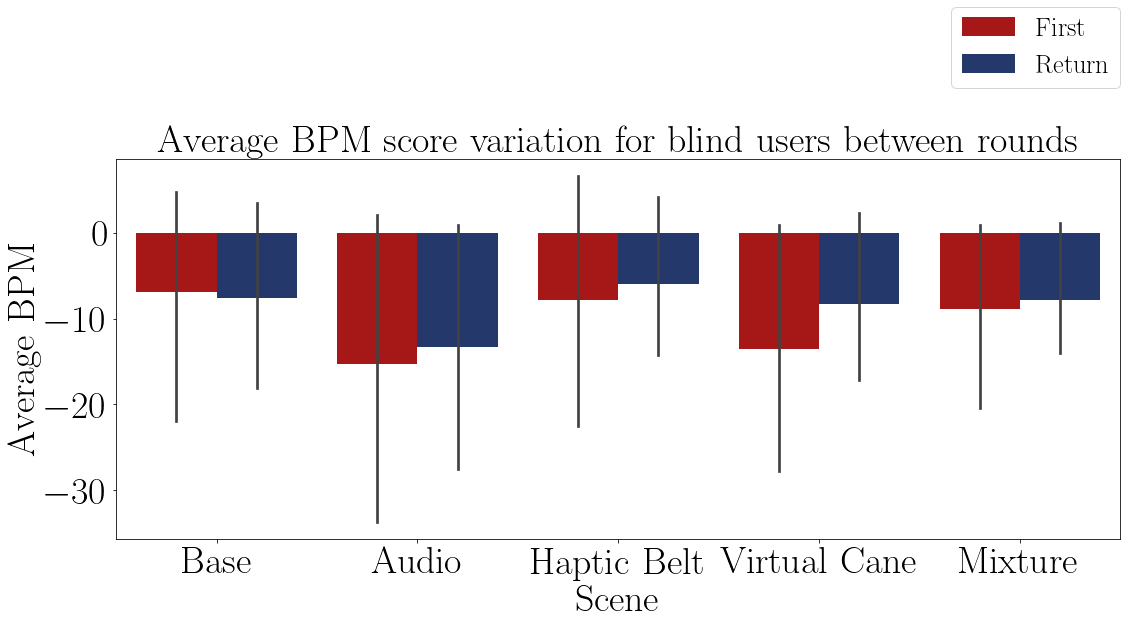
\includegraphics[width = 0.8\linewidth]{Resultados/ECG/Figuras/png/barplot_ecg_bpm_scene_blind.png}
        %\resizebox{0.8\linewidth}{!}{
        %%% Creator: Matplotlib, PGF backend
%%
%% To include the figure in your LaTeX document, write
%%   \input{<filename>.pgf}
%%
%% Make sure the required packages are loaded in your preamble
%%   \usepackage{pgf}
%%
%% Figures using additional raster images can only be included by \input if
%% they are in the same directory as the main LaTeX file. For loading figures
%% from other directories you can use the `import` package
%%   \usepackage{import}
%%
%% and then include the figures with
%%   \import{<path to file>}{<filename>.pgf}
%%
%% Matplotlib used the following preamble
%%   \usepackage{fontspec}
%%
\begingroup%
\makeatletter%
\begin{pgfpicture}%
\pgfpathrectangle{\pgfpointorigin}{\pgfqpoint{15.369508in}{8.690562in}}%
\pgfusepath{use as bounding box, clip}%
\begin{pgfscope}%
\pgfsetbuttcap%
\pgfsetmiterjoin%
\pgfsetlinewidth{0.000000pt}%
\definecolor{currentstroke}{rgb}{1.000000,1.000000,1.000000}%
\pgfsetstrokecolor{currentstroke}%
\pgfsetstrokeopacity{0.000000}%
\pgfsetdash{}{0pt}%
\pgfpathmoveto{\pgfqpoint{0.000000in}{-0.000000in}}%
\pgfpathlineto{\pgfqpoint{15.369508in}{-0.000000in}}%
\pgfpathlineto{\pgfqpoint{15.369508in}{8.690562in}}%
\pgfpathlineto{\pgfqpoint{0.000000in}{8.690562in}}%
\pgfpathclose%
\pgfusepath{}%
\end{pgfscope}%
\begin{pgfscope}%
\pgfsetbuttcap%
\pgfsetmiterjoin%
\definecolor{currentfill}{rgb}{1.000000,1.000000,1.000000}%
\pgfsetfillcolor{currentfill}%
\pgfsetlinewidth{0.000000pt}%
\definecolor{currentstroke}{rgb}{0.000000,0.000000,0.000000}%
\pgfsetstrokecolor{currentstroke}%
\pgfsetstrokeopacity{0.000000}%
\pgfsetdash{}{0pt}%
\pgfpathmoveto{\pgfqpoint{1.319508in}{1.191562in}}%
\pgfpathlineto{\pgfqpoint{15.269508in}{1.191562in}}%
\pgfpathlineto{\pgfqpoint{15.269508in}{6.476562in}}%
\pgfpathlineto{\pgfqpoint{1.319508in}{6.476562in}}%
\pgfpathclose%
\pgfusepath{fill}%
\end{pgfscope}%
\begin{pgfscope}%
\pgfpathrectangle{\pgfqpoint{1.319508in}{1.191562in}}{\pgfqpoint{13.950000in}{5.285000in}}%
\pgfusepath{clip}%
\pgfsetbuttcap%
\pgfsetmiterjoin%
\definecolor{currentfill}{rgb}{0.651961,0.093137,0.093137}%
\pgfsetfillcolor{currentfill}%
\pgfsetlinewidth{0.000000pt}%
\definecolor{currentstroke}{rgb}{0.000000,0.000000,0.000000}%
\pgfsetstrokecolor{currentstroke}%
\pgfsetstrokeopacity{0.000000}%
\pgfsetdash{}{0pt}%
\pgfpathmoveto{\pgfqpoint{1.598508in}{5.432025in}}%
\pgfpathlineto{\pgfqpoint{2.714508in}{5.432025in}}%
\pgfpathlineto{\pgfqpoint{2.714508in}{4.583309in}}%
\pgfpathlineto{\pgfqpoint{1.598508in}{4.583309in}}%
\pgfpathclose%
\pgfusepath{fill}%
\end{pgfscope}%
\begin{pgfscope}%
\pgfpathrectangle{\pgfqpoint{1.319508in}{1.191562in}}{\pgfqpoint{13.950000in}{5.285000in}}%
\pgfusepath{clip}%
\pgfsetbuttcap%
\pgfsetmiterjoin%
\definecolor{currentfill}{rgb}{0.651961,0.093137,0.093137}%
\pgfsetfillcolor{currentfill}%
\pgfsetlinewidth{0.000000pt}%
\definecolor{currentstroke}{rgb}{0.000000,0.000000,0.000000}%
\pgfsetstrokecolor{currentstroke}%
\pgfsetstrokeopacity{0.000000}%
\pgfsetdash{}{0pt}%
\pgfpathmoveto{\pgfqpoint{4.388508in}{5.432025in}}%
\pgfpathlineto{\pgfqpoint{5.504508in}{5.432025in}}%
\pgfpathlineto{\pgfqpoint{5.504508in}{3.558465in}}%
\pgfpathlineto{\pgfqpoint{4.388508in}{3.558465in}}%
\pgfpathclose%
\pgfusepath{fill}%
\end{pgfscope}%
\begin{pgfscope}%
\pgfpathrectangle{\pgfqpoint{1.319508in}{1.191562in}}{\pgfqpoint{13.950000in}{5.285000in}}%
\pgfusepath{clip}%
\pgfsetbuttcap%
\pgfsetmiterjoin%
\definecolor{currentfill}{rgb}{0.651961,0.093137,0.093137}%
\pgfsetfillcolor{currentfill}%
\pgfsetlinewidth{0.000000pt}%
\definecolor{currentstroke}{rgb}{0.000000,0.000000,0.000000}%
\pgfsetstrokecolor{currentstroke}%
\pgfsetstrokeopacity{0.000000}%
\pgfsetdash{}{0pt}%
\pgfpathmoveto{\pgfqpoint{7.178508in}{5.432025in}}%
\pgfpathlineto{\pgfqpoint{8.294508in}{5.432025in}}%
\pgfpathlineto{\pgfqpoint{8.294508in}{4.476572in}}%
\pgfpathlineto{\pgfqpoint{7.178508in}{4.476572in}}%
\pgfpathclose%
\pgfusepath{fill}%
\end{pgfscope}%
\begin{pgfscope}%
\pgfpathrectangle{\pgfqpoint{1.319508in}{1.191562in}}{\pgfqpoint{13.950000in}{5.285000in}}%
\pgfusepath{clip}%
\pgfsetbuttcap%
\pgfsetmiterjoin%
\definecolor{currentfill}{rgb}{0.651961,0.093137,0.093137}%
\pgfsetfillcolor{currentfill}%
\pgfsetlinewidth{0.000000pt}%
\definecolor{currentstroke}{rgb}{0.000000,0.000000,0.000000}%
\pgfsetstrokecolor{currentstroke}%
\pgfsetstrokeopacity{0.000000}%
\pgfsetdash{}{0pt}%
\pgfpathmoveto{\pgfqpoint{9.968508in}{5.432025in}}%
\pgfpathlineto{\pgfqpoint{11.084508in}{5.432025in}}%
\pgfpathlineto{\pgfqpoint{11.084508in}{3.778608in}}%
\pgfpathlineto{\pgfqpoint{9.968508in}{3.778608in}}%
\pgfpathclose%
\pgfusepath{fill}%
\end{pgfscope}%
\begin{pgfscope}%
\pgfpathrectangle{\pgfqpoint{1.319508in}{1.191562in}}{\pgfqpoint{13.950000in}{5.285000in}}%
\pgfusepath{clip}%
\pgfsetbuttcap%
\pgfsetmiterjoin%
\definecolor{currentfill}{rgb}{0.651961,0.093137,0.093137}%
\pgfsetfillcolor{currentfill}%
\pgfsetlinewidth{0.000000pt}%
\definecolor{currentstroke}{rgb}{0.000000,0.000000,0.000000}%
\pgfsetstrokecolor{currentstroke}%
\pgfsetstrokeopacity{0.000000}%
\pgfsetdash{}{0pt}%
\pgfpathmoveto{\pgfqpoint{12.758508in}{5.432025in}}%
\pgfpathlineto{\pgfqpoint{13.874508in}{5.432025in}}%
\pgfpathlineto{\pgfqpoint{13.874508in}{4.339698in}}%
\pgfpathlineto{\pgfqpoint{12.758508in}{4.339698in}}%
\pgfpathclose%
\pgfusepath{fill}%
\end{pgfscope}%
\begin{pgfscope}%
\pgfpathrectangle{\pgfqpoint{1.319508in}{1.191562in}}{\pgfqpoint{13.950000in}{5.285000in}}%
\pgfusepath{clip}%
\pgfsetbuttcap%
\pgfsetmiterjoin%
\definecolor{currentfill}{rgb}{0.144608,0.218137,0.424020}%
\pgfsetfillcolor{currentfill}%
\pgfsetlinewidth{0.000000pt}%
\definecolor{currentstroke}{rgb}{0.000000,0.000000,0.000000}%
\pgfsetstrokecolor{currentstroke}%
\pgfsetstrokeopacity{0.000000}%
\pgfsetdash{}{0pt}%
\pgfpathmoveto{\pgfqpoint{2.714508in}{5.432025in}}%
\pgfpathlineto{\pgfqpoint{3.830508in}{5.432025in}}%
\pgfpathlineto{\pgfqpoint{3.830508in}{4.506389in}}%
\pgfpathlineto{\pgfqpoint{2.714508in}{4.506389in}}%
\pgfpathclose%
\pgfusepath{fill}%
\end{pgfscope}%
\begin{pgfscope}%
\pgfpathrectangle{\pgfqpoint{1.319508in}{1.191562in}}{\pgfqpoint{13.950000in}{5.285000in}}%
\pgfusepath{clip}%
\pgfsetbuttcap%
\pgfsetmiterjoin%
\definecolor{currentfill}{rgb}{0.144608,0.218137,0.424020}%
\pgfsetfillcolor{currentfill}%
\pgfsetlinewidth{0.000000pt}%
\definecolor{currentstroke}{rgb}{0.000000,0.000000,0.000000}%
\pgfsetstrokecolor{currentstroke}%
\pgfsetstrokeopacity{0.000000}%
\pgfsetdash{}{0pt}%
\pgfpathmoveto{\pgfqpoint{5.504508in}{5.432025in}}%
\pgfpathlineto{\pgfqpoint{6.620508in}{5.432025in}}%
\pgfpathlineto{\pgfqpoint{6.620508in}{3.808164in}}%
\pgfpathlineto{\pgfqpoint{5.504508in}{3.808164in}}%
\pgfpathclose%
\pgfusepath{fill}%
\end{pgfscope}%
\begin{pgfscope}%
\pgfpathrectangle{\pgfqpoint{1.319508in}{1.191562in}}{\pgfqpoint{13.950000in}{5.285000in}}%
\pgfusepath{clip}%
\pgfsetbuttcap%
\pgfsetmiterjoin%
\definecolor{currentfill}{rgb}{0.144608,0.218137,0.424020}%
\pgfsetfillcolor{currentfill}%
\pgfsetlinewidth{0.000000pt}%
\definecolor{currentstroke}{rgb}{0.000000,0.000000,0.000000}%
\pgfsetstrokecolor{currentstroke}%
\pgfsetstrokeopacity{0.000000}%
\pgfsetdash{}{0pt}%
\pgfpathmoveto{\pgfqpoint{8.294508in}{5.432025in}}%
\pgfpathlineto{\pgfqpoint{9.410508in}{5.432025in}}%
\pgfpathlineto{\pgfqpoint{9.410508in}{4.696413in}}%
\pgfpathlineto{\pgfqpoint{8.294508in}{4.696413in}}%
\pgfpathclose%
\pgfusepath{fill}%
\end{pgfscope}%
\begin{pgfscope}%
\pgfpathrectangle{\pgfqpoint{1.319508in}{1.191562in}}{\pgfqpoint{13.950000in}{5.285000in}}%
\pgfusepath{clip}%
\pgfsetbuttcap%
\pgfsetmiterjoin%
\definecolor{currentfill}{rgb}{0.144608,0.218137,0.424020}%
\pgfsetfillcolor{currentfill}%
\pgfsetlinewidth{0.000000pt}%
\definecolor{currentstroke}{rgb}{0.000000,0.000000,0.000000}%
\pgfsetstrokecolor{currentstroke}%
\pgfsetstrokeopacity{0.000000}%
\pgfsetdash{}{0pt}%
\pgfpathmoveto{\pgfqpoint{11.084508in}{5.432025in}}%
\pgfpathlineto{\pgfqpoint{12.200508in}{5.432025in}}%
\pgfpathlineto{\pgfqpoint{12.200508in}{4.423975in}}%
\pgfpathlineto{\pgfqpoint{11.084508in}{4.423975in}}%
\pgfpathclose%
\pgfusepath{fill}%
\end{pgfscope}%
\begin{pgfscope}%
\pgfpathrectangle{\pgfqpoint{1.319508in}{1.191562in}}{\pgfqpoint{13.950000in}{5.285000in}}%
\pgfusepath{clip}%
\pgfsetbuttcap%
\pgfsetmiterjoin%
\definecolor{currentfill}{rgb}{0.144608,0.218137,0.424020}%
\pgfsetfillcolor{currentfill}%
\pgfsetlinewidth{0.000000pt}%
\definecolor{currentstroke}{rgb}{0.000000,0.000000,0.000000}%
\pgfsetstrokecolor{currentstroke}%
\pgfsetstrokeopacity{0.000000}%
\pgfsetdash{}{0pt}%
\pgfpathmoveto{\pgfqpoint{13.874508in}{5.432025in}}%
\pgfpathlineto{\pgfqpoint{14.990508in}{5.432025in}}%
\pgfpathlineto{\pgfqpoint{14.990508in}{4.469000in}}%
\pgfpathlineto{\pgfqpoint{13.874508in}{4.469000in}}%
\pgfpathclose%
\pgfusepath{fill}%
\end{pgfscope}%
\begin{pgfscope}%
\pgfsetbuttcap%
\pgfsetroundjoin%
\definecolor{currentfill}{rgb}{0.000000,0.000000,0.000000}%
\pgfsetfillcolor{currentfill}%
\pgfsetlinewidth{0.803000pt}%
\definecolor{currentstroke}{rgb}{0.000000,0.000000,0.000000}%
\pgfsetstrokecolor{currentstroke}%
\pgfsetdash{}{0pt}%
\pgfsys@defobject{currentmarker}{\pgfqpoint{0.000000in}{-0.048611in}}{\pgfqpoint{0.000000in}{0.000000in}}{%
\pgfpathmoveto{\pgfqpoint{0.000000in}{0.000000in}}%
\pgfpathlineto{\pgfqpoint{0.000000in}{-0.048611in}}%
\pgfusepath{stroke,fill}%
}%
\begin{pgfscope}%
\pgfsys@transformshift{2.714508in}{1.191562in}%
\pgfsys@useobject{currentmarker}{}%
\end{pgfscope}%
\end{pgfscope}%
\begin{pgfscope}%
\definecolor{textcolor}{rgb}{0.000000,0.000000,0.000000}%
\pgfsetstrokecolor{textcolor}%
\pgfsetfillcolor{textcolor}%
\pgftext[x=2.714508in,y=1.094339in,,top]{\color{textcolor}\rmfamily\fontsize{38.016000}{45.619200}\selectfont Base}%
\end{pgfscope}%
\begin{pgfscope}%
\pgfsetbuttcap%
\pgfsetroundjoin%
\definecolor{currentfill}{rgb}{0.000000,0.000000,0.000000}%
\pgfsetfillcolor{currentfill}%
\pgfsetlinewidth{0.803000pt}%
\definecolor{currentstroke}{rgb}{0.000000,0.000000,0.000000}%
\pgfsetstrokecolor{currentstroke}%
\pgfsetdash{}{0pt}%
\pgfsys@defobject{currentmarker}{\pgfqpoint{0.000000in}{-0.048611in}}{\pgfqpoint{0.000000in}{0.000000in}}{%
\pgfpathmoveto{\pgfqpoint{0.000000in}{0.000000in}}%
\pgfpathlineto{\pgfqpoint{0.000000in}{-0.048611in}}%
\pgfusepath{stroke,fill}%
}%
\begin{pgfscope}%
\pgfsys@transformshift{5.504508in}{1.191562in}%
\pgfsys@useobject{currentmarker}{}%
\end{pgfscope}%
\end{pgfscope}%
\begin{pgfscope}%
\definecolor{textcolor}{rgb}{0.000000,0.000000,0.000000}%
\pgfsetstrokecolor{textcolor}%
\pgfsetfillcolor{textcolor}%
\pgftext[x=5.504508in,y=1.094339in,,top]{\color{textcolor}\rmfamily\fontsize{38.016000}{45.619200}\selectfont Audio}%
\end{pgfscope}%
\begin{pgfscope}%
\pgfsetbuttcap%
\pgfsetroundjoin%
\definecolor{currentfill}{rgb}{0.000000,0.000000,0.000000}%
\pgfsetfillcolor{currentfill}%
\pgfsetlinewidth{0.803000pt}%
\definecolor{currentstroke}{rgb}{0.000000,0.000000,0.000000}%
\pgfsetstrokecolor{currentstroke}%
\pgfsetdash{}{0pt}%
\pgfsys@defobject{currentmarker}{\pgfqpoint{0.000000in}{-0.048611in}}{\pgfqpoint{0.000000in}{0.000000in}}{%
\pgfpathmoveto{\pgfqpoint{0.000000in}{0.000000in}}%
\pgfpathlineto{\pgfqpoint{0.000000in}{-0.048611in}}%
\pgfusepath{stroke,fill}%
}%
\begin{pgfscope}%
\pgfsys@transformshift{8.294508in}{1.191562in}%
\pgfsys@useobject{currentmarker}{}%
\end{pgfscope}%
\end{pgfscope}%
\begin{pgfscope}%
\definecolor{textcolor}{rgb}{0.000000,0.000000,0.000000}%
\pgfsetstrokecolor{textcolor}%
\pgfsetfillcolor{textcolor}%
\pgftext[x=8.294508in,y=1.094339in,,top]{\color{textcolor}\rmfamily\fontsize{38.016000}{45.619200}\selectfont Haptic Belt}%
\end{pgfscope}%
\begin{pgfscope}%
\pgfsetbuttcap%
\pgfsetroundjoin%
\definecolor{currentfill}{rgb}{0.000000,0.000000,0.000000}%
\pgfsetfillcolor{currentfill}%
\pgfsetlinewidth{0.803000pt}%
\definecolor{currentstroke}{rgb}{0.000000,0.000000,0.000000}%
\pgfsetstrokecolor{currentstroke}%
\pgfsetdash{}{0pt}%
\pgfsys@defobject{currentmarker}{\pgfqpoint{0.000000in}{-0.048611in}}{\pgfqpoint{0.000000in}{0.000000in}}{%
\pgfpathmoveto{\pgfqpoint{0.000000in}{0.000000in}}%
\pgfpathlineto{\pgfqpoint{0.000000in}{-0.048611in}}%
\pgfusepath{stroke,fill}%
}%
\begin{pgfscope}%
\pgfsys@transformshift{11.084508in}{1.191562in}%
\pgfsys@useobject{currentmarker}{}%
\end{pgfscope}%
\end{pgfscope}%
\begin{pgfscope}%
\definecolor{textcolor}{rgb}{0.000000,0.000000,0.000000}%
\pgfsetstrokecolor{textcolor}%
\pgfsetfillcolor{textcolor}%
\pgftext[x=11.084508in,y=1.094339in,,top]{\color{textcolor}\rmfamily\fontsize{38.016000}{45.619200}\selectfont Virtual Cane}%
\end{pgfscope}%
\begin{pgfscope}%
\pgfsetbuttcap%
\pgfsetroundjoin%
\definecolor{currentfill}{rgb}{0.000000,0.000000,0.000000}%
\pgfsetfillcolor{currentfill}%
\pgfsetlinewidth{0.803000pt}%
\definecolor{currentstroke}{rgb}{0.000000,0.000000,0.000000}%
\pgfsetstrokecolor{currentstroke}%
\pgfsetdash{}{0pt}%
\pgfsys@defobject{currentmarker}{\pgfqpoint{0.000000in}{-0.048611in}}{\pgfqpoint{0.000000in}{0.000000in}}{%
\pgfpathmoveto{\pgfqpoint{0.000000in}{0.000000in}}%
\pgfpathlineto{\pgfqpoint{0.000000in}{-0.048611in}}%
\pgfusepath{stroke,fill}%
}%
\begin{pgfscope}%
\pgfsys@transformshift{13.874508in}{1.191562in}%
\pgfsys@useobject{currentmarker}{}%
\end{pgfscope}%
\end{pgfscope}%
\begin{pgfscope}%
\definecolor{textcolor}{rgb}{0.000000,0.000000,0.000000}%
\pgfsetstrokecolor{textcolor}%
\pgfsetfillcolor{textcolor}%
\pgftext[x=13.874508in,y=1.094339in,,top]{\color{textcolor}\rmfamily\fontsize{38.016000}{45.619200}\selectfont Mixture}%
\end{pgfscope}%
\begin{pgfscope}%
\definecolor{textcolor}{rgb}{0.000000,0.000000,0.000000}%
\pgfsetstrokecolor{textcolor}%
\pgfsetfillcolor{textcolor}%
\pgftext[x=8.294508in,y=0.569392in,,top]{\color{textcolor}\rmfamily\fontsize{38.016000}{45.619200}\selectfont Scene}%
\end{pgfscope}%
\begin{pgfscope}%
\pgfsetbuttcap%
\pgfsetroundjoin%
\definecolor{currentfill}{rgb}{0.000000,0.000000,0.000000}%
\pgfsetfillcolor{currentfill}%
\pgfsetlinewidth{0.803000pt}%
\definecolor{currentstroke}{rgb}{0.000000,0.000000,0.000000}%
\pgfsetstrokecolor{currentstroke}%
\pgfsetdash{}{0pt}%
\pgfsys@defobject{currentmarker}{\pgfqpoint{-0.048611in}{0.000000in}}{\pgfqpoint{-0.000000in}{0.000000in}}{%
\pgfpathmoveto{\pgfqpoint{-0.000000in}{0.000000in}}%
\pgfpathlineto{\pgfqpoint{-0.048611in}{0.000000in}}%
\pgfusepath{stroke,fill}%
}%
\begin{pgfscope}%
\pgfsys@transformshift{1.319508in}{1.767373in}%
\pgfsys@useobject{currentmarker}{}%
\end{pgfscope}%
\end{pgfscope}%
\begin{pgfscope}%
\definecolor{textcolor}{rgb}{0.000000,0.000000,0.000000}%
\pgfsetstrokecolor{textcolor}%
\pgfsetfillcolor{textcolor}%
\pgftext[x=0.636563in, y=1.584157in, left, base]{\color{textcolor}\rmfamily\fontsize{38.016000}{45.619200}\selectfont \(\displaystyle {\ensuremath{-}30}\)}%
\end{pgfscope}%
\begin{pgfscope}%
\pgfsetbuttcap%
\pgfsetroundjoin%
\definecolor{currentfill}{rgb}{0.000000,0.000000,0.000000}%
\pgfsetfillcolor{currentfill}%
\pgfsetlinewidth{0.803000pt}%
\definecolor{currentstroke}{rgb}{0.000000,0.000000,0.000000}%
\pgfsetstrokecolor{currentstroke}%
\pgfsetdash{}{0pt}%
\pgfsys@defobject{currentmarker}{\pgfqpoint{-0.048611in}{0.000000in}}{\pgfqpoint{-0.000000in}{0.000000in}}{%
\pgfpathmoveto{\pgfqpoint{-0.000000in}{0.000000in}}%
\pgfpathlineto{\pgfqpoint{-0.048611in}{0.000000in}}%
\pgfusepath{stroke,fill}%
}%
\begin{pgfscope}%
\pgfsys@transformshift{1.319508in}{2.988924in}%
\pgfsys@useobject{currentmarker}{}%
\end{pgfscope}%
\end{pgfscope}%
\begin{pgfscope}%
\definecolor{textcolor}{rgb}{0.000000,0.000000,0.000000}%
\pgfsetstrokecolor{textcolor}%
\pgfsetfillcolor{textcolor}%
\pgftext[x=0.636563in, y=2.805708in, left, base]{\color{textcolor}\rmfamily\fontsize{38.016000}{45.619200}\selectfont \(\displaystyle {\ensuremath{-}20}\)}%
\end{pgfscope}%
\begin{pgfscope}%
\pgfsetbuttcap%
\pgfsetroundjoin%
\definecolor{currentfill}{rgb}{0.000000,0.000000,0.000000}%
\pgfsetfillcolor{currentfill}%
\pgfsetlinewidth{0.803000pt}%
\definecolor{currentstroke}{rgb}{0.000000,0.000000,0.000000}%
\pgfsetstrokecolor{currentstroke}%
\pgfsetdash{}{0pt}%
\pgfsys@defobject{currentmarker}{\pgfqpoint{-0.048611in}{0.000000in}}{\pgfqpoint{-0.000000in}{0.000000in}}{%
\pgfpathmoveto{\pgfqpoint{-0.000000in}{0.000000in}}%
\pgfpathlineto{\pgfqpoint{-0.048611in}{0.000000in}}%
\pgfusepath{stroke,fill}%
}%
\begin{pgfscope}%
\pgfsys@transformshift{1.319508in}{4.210475in}%
\pgfsys@useobject{currentmarker}{}%
\end{pgfscope}%
\end{pgfscope}%
\begin{pgfscope}%
\definecolor{textcolor}{rgb}{0.000000,0.000000,0.000000}%
\pgfsetstrokecolor{textcolor}%
\pgfsetfillcolor{textcolor}%
\pgftext[x=0.636563in, y=4.027258in, left, base]{\color{textcolor}\rmfamily\fontsize{38.016000}{45.619200}\selectfont \(\displaystyle {\ensuremath{-}10}\)}%
\end{pgfscope}%
\begin{pgfscope}%
\pgfsetbuttcap%
\pgfsetroundjoin%
\definecolor{currentfill}{rgb}{0.000000,0.000000,0.000000}%
\pgfsetfillcolor{currentfill}%
\pgfsetlinewidth{0.803000pt}%
\definecolor{currentstroke}{rgb}{0.000000,0.000000,0.000000}%
\pgfsetstrokecolor{currentstroke}%
\pgfsetdash{}{0pt}%
\pgfsys@defobject{currentmarker}{\pgfqpoint{-0.048611in}{0.000000in}}{\pgfqpoint{-0.000000in}{0.000000in}}{%
\pgfpathmoveto{\pgfqpoint{-0.000000in}{0.000000in}}%
\pgfpathlineto{\pgfqpoint{-0.048611in}{0.000000in}}%
\pgfusepath{stroke,fill}%
}%
\begin{pgfscope}%
\pgfsys@transformshift{1.319508in}{5.432025in}%
\pgfsys@useobject{currentmarker}{}%
\end{pgfscope}%
\end{pgfscope}%
\begin{pgfscope}%
\definecolor{textcolor}{rgb}{0.000000,0.000000,0.000000}%
\pgfsetstrokecolor{textcolor}%
\pgfsetfillcolor{textcolor}%
\pgftext[x=1.063808in, y=5.248809in, left, base]{\color{textcolor}\rmfamily\fontsize{38.016000}{45.619200}\selectfont \(\displaystyle {0}\)}%
\end{pgfscope}%
\begin{pgfscope}%
\definecolor{textcolor}{rgb}{0.000000,0.000000,0.000000}%
\pgfsetstrokecolor{textcolor}%
\pgfsetfillcolor{textcolor}%
\pgftext[x=0.581008in,y=3.834062in,,bottom,rotate=90.000000]{\color{textcolor}\rmfamily\fontsize{38.016000}{45.619200}\selectfont Average BPM}%
\end{pgfscope}%
\begin{pgfscope}%
\pgfpathrectangle{\pgfqpoint{1.319508in}{1.191562in}}{\pgfqpoint{13.950000in}{5.285000in}}%
\pgfusepath{clip}%
\pgfsetrectcap%
\pgfsetroundjoin%
\pgfsetlinewidth{2.710125pt}%
\definecolor{currentstroke}{rgb}{0.260000,0.260000,0.260000}%
\pgfsetstrokecolor{currentstroke}%
\pgfsetdash{}{0pt}%
\pgfpathmoveto{\pgfqpoint{2.156508in}{2.751308in}}%
\pgfpathlineto{\pgfqpoint{2.156508in}{6.018483in}}%
\pgfusepath{stroke}%
\end{pgfscope}%
\begin{pgfscope}%
\pgfpathrectangle{\pgfqpoint{1.319508in}{1.191562in}}{\pgfqpoint{13.950000in}{5.285000in}}%
\pgfusepath{clip}%
\pgfsetrectcap%
\pgfsetroundjoin%
\pgfsetlinewidth{2.710125pt}%
\definecolor{currentstroke}{rgb}{0.260000,0.260000,0.260000}%
\pgfsetstrokecolor{currentstroke}%
\pgfsetdash{}{0pt}%
\pgfpathmoveto{\pgfqpoint{4.946508in}{1.431789in}}%
\pgfpathlineto{\pgfqpoint{4.946508in}{5.682086in}}%
\pgfusepath{stroke}%
\end{pgfscope}%
\begin{pgfscope}%
\pgfpathrectangle{\pgfqpoint{1.319508in}{1.191562in}}{\pgfqpoint{13.950000in}{5.285000in}}%
\pgfusepath{clip}%
\pgfsetrectcap%
\pgfsetroundjoin%
\pgfsetlinewidth{2.710125pt}%
\definecolor{currentstroke}{rgb}{0.260000,0.260000,0.260000}%
\pgfsetstrokecolor{currentstroke}%
\pgfsetdash{}{0pt}%
\pgfpathmoveto{\pgfqpoint{7.736508in}{2.678943in}}%
\pgfpathlineto{\pgfqpoint{7.736508in}{6.236334in}}%
\pgfusepath{stroke}%
\end{pgfscope}%
\begin{pgfscope}%
\pgfpathrectangle{\pgfqpoint{1.319508in}{1.191562in}}{\pgfqpoint{13.950000in}{5.285000in}}%
\pgfusepath{clip}%
\pgfsetrectcap%
\pgfsetroundjoin%
\pgfsetlinewidth{2.710125pt}%
\definecolor{currentstroke}{rgb}{0.260000,0.260000,0.260000}%
\pgfsetstrokecolor{currentstroke}%
\pgfsetdash{}{0pt}%
\pgfpathmoveto{\pgfqpoint{10.526508in}{2.047721in}}%
\pgfpathlineto{\pgfqpoint{10.526508in}{5.510294in}}%
\pgfusepath{stroke}%
\end{pgfscope}%
\begin{pgfscope}%
\pgfpathrectangle{\pgfqpoint{1.319508in}{1.191562in}}{\pgfqpoint{13.950000in}{5.285000in}}%
\pgfusepath{clip}%
\pgfsetrectcap%
\pgfsetroundjoin%
\pgfsetlinewidth{2.710125pt}%
\definecolor{currentstroke}{rgb}{0.260000,0.260000,0.260000}%
\pgfsetstrokecolor{currentstroke}%
\pgfsetdash{}{0pt}%
\pgfpathmoveto{\pgfqpoint{13.316508in}{3.163834in}}%
\pgfpathlineto{\pgfqpoint{13.316508in}{5.543100in}}%
\pgfusepath{stroke}%
\end{pgfscope}%
\begin{pgfscope}%
\pgfpathrectangle{\pgfqpoint{1.319508in}{1.191562in}}{\pgfqpoint{13.950000in}{5.285000in}}%
\pgfusepath{clip}%
\pgfsetrectcap%
\pgfsetroundjoin%
\pgfsetlinewidth{2.710125pt}%
\definecolor{currentstroke}{rgb}{0.260000,0.260000,0.260000}%
\pgfsetstrokecolor{currentstroke}%
\pgfsetdash{}{0pt}%
\pgfpathmoveto{\pgfqpoint{3.272508in}{3.222854in}}%
\pgfpathlineto{\pgfqpoint{3.272508in}{5.709606in}}%
\pgfusepath{stroke}%
\end{pgfscope}%
\begin{pgfscope}%
\pgfpathrectangle{\pgfqpoint{1.319508in}{1.191562in}}{\pgfqpoint{13.950000in}{5.285000in}}%
\pgfusepath{clip}%
\pgfsetrectcap%
\pgfsetroundjoin%
\pgfsetlinewidth{2.710125pt}%
\definecolor{currentstroke}{rgb}{0.260000,0.260000,0.260000}%
\pgfsetstrokecolor{currentstroke}%
\pgfsetdash{}{0pt}%
\pgfpathmoveto{\pgfqpoint{6.062508in}{1.933256in}}%
\pgfpathlineto{\pgfqpoint{6.062508in}{5.541904in}}%
\pgfusepath{stroke}%
\end{pgfscope}%
\begin{pgfscope}%
\pgfpathrectangle{\pgfqpoint{1.319508in}{1.191562in}}{\pgfqpoint{13.950000in}{5.285000in}}%
\pgfusepath{clip}%
\pgfsetrectcap%
\pgfsetroundjoin%
\pgfsetlinewidth{2.710125pt}%
\definecolor{currentstroke}{rgb}{0.260000,0.260000,0.260000}%
\pgfsetstrokecolor{currentstroke}%
\pgfsetdash{}{0pt}%
\pgfpathmoveto{\pgfqpoint{8.852508in}{3.694214in}}%
\pgfpathlineto{\pgfqpoint{8.852508in}{5.935485in}}%
\pgfusepath{stroke}%
\end{pgfscope}%
\begin{pgfscope}%
\pgfpathrectangle{\pgfqpoint{1.319508in}{1.191562in}}{\pgfqpoint{13.950000in}{5.285000in}}%
\pgfusepath{clip}%
\pgfsetrectcap%
\pgfsetroundjoin%
\pgfsetlinewidth{2.710125pt}%
\definecolor{currentstroke}{rgb}{0.260000,0.260000,0.260000}%
\pgfsetstrokecolor{currentstroke}%
\pgfsetdash{}{0pt}%
\pgfpathmoveto{\pgfqpoint{11.642508in}{3.336183in}}%
\pgfpathlineto{\pgfqpoint{11.642508in}{5.657013in}}%
\pgfusepath{stroke}%
\end{pgfscope}%
\begin{pgfscope}%
\pgfpathrectangle{\pgfqpoint{1.319508in}{1.191562in}}{\pgfqpoint{13.950000in}{5.285000in}}%
\pgfusepath{clip}%
\pgfsetrectcap%
\pgfsetroundjoin%
\pgfsetlinewidth{2.710125pt}%
\definecolor{currentstroke}{rgb}{0.260000,0.260000,0.260000}%
\pgfsetstrokecolor{currentstroke}%
\pgfsetdash{}{0pt}%
\pgfpathmoveto{\pgfqpoint{14.432508in}{3.718499in}}%
\pgfpathlineto{\pgfqpoint{14.432508in}{5.571045in}}%
\pgfusepath{stroke}%
\end{pgfscope}%
\begin{pgfscope}%
\pgfsetrectcap%
\pgfsetmiterjoin%
\pgfsetlinewidth{0.803000pt}%
\definecolor{currentstroke}{rgb}{0.000000,0.000000,0.000000}%
\pgfsetstrokecolor{currentstroke}%
\pgfsetdash{}{0pt}%
\pgfpathmoveto{\pgfqpoint{1.319508in}{1.191562in}}%
\pgfpathlineto{\pgfqpoint{1.319508in}{6.476562in}}%
\pgfusepath{stroke}%
\end{pgfscope}%
\begin{pgfscope}%
\pgfsetrectcap%
\pgfsetmiterjoin%
\pgfsetlinewidth{0.803000pt}%
\definecolor{currentstroke}{rgb}{0.000000,0.000000,0.000000}%
\pgfsetstrokecolor{currentstroke}%
\pgfsetdash{}{0pt}%
\pgfpathmoveto{\pgfqpoint{15.269508in}{1.191562in}}%
\pgfpathlineto{\pgfqpoint{15.269508in}{6.476562in}}%
\pgfusepath{stroke}%
\end{pgfscope}%
\begin{pgfscope}%
\pgfsetrectcap%
\pgfsetmiterjoin%
\pgfsetlinewidth{0.803000pt}%
\definecolor{currentstroke}{rgb}{0.000000,0.000000,0.000000}%
\pgfsetstrokecolor{currentstroke}%
\pgfsetdash{}{0pt}%
\pgfpathmoveto{\pgfqpoint{1.319508in}{1.191562in}}%
\pgfpathlineto{\pgfqpoint{15.269508in}{1.191562in}}%
\pgfusepath{stroke}%
\end{pgfscope}%
\begin{pgfscope}%
\pgfsetrectcap%
\pgfsetmiterjoin%
\pgfsetlinewidth{0.803000pt}%
\definecolor{currentstroke}{rgb}{0.000000,0.000000,0.000000}%
\pgfsetstrokecolor{currentstroke}%
\pgfsetdash{}{0pt}%
\pgfpathmoveto{\pgfqpoint{1.319508in}{6.476562in}}%
\pgfpathlineto{\pgfqpoint{15.269508in}{6.476562in}}%
\pgfusepath{stroke}%
\end{pgfscope}%
\begin{pgfscope}%
\definecolor{textcolor}{rgb}{0.000000,0.000000,0.000000}%
\pgfsetstrokecolor{textcolor}%
\pgfsetfillcolor{textcolor}%
\pgftext[x=8.294508in,y=6.584273in,,base]{\color{textcolor}\rmfamily\fontsize{38.016000}{45.619200}\selectfont Average BPM score variation for blind users between rounds}%
\end{pgfscope}%
\begin{pgfscope}%
\pgfsetbuttcap%
\pgfsetmiterjoin%
\definecolor{currentfill}{rgb}{1.000000,1.000000,1.000000}%
\pgfsetfillcolor{currentfill}%
\pgfsetfillopacity{0.800000}%
\pgfsetlinewidth{1.003750pt}%
\definecolor{currentstroke}{rgb}{0.800000,0.800000,0.800000}%
\pgfsetstrokecolor{currentstroke}%
\pgfsetstrokeopacity{0.800000}%
\pgfsetdash{}{0pt}%
\pgfpathmoveto{\pgfqpoint{12.990308in}{7.457562in}}%
\pgfpathlineto{\pgfqpoint{15.196175in}{7.457562in}}%
\pgfpathquadraticcurveto{\pgfqpoint{15.269508in}{7.457562in}}{\pgfqpoint{15.269508in}{7.530896in}}%
\pgfpathlineto{\pgfqpoint{15.269508in}{8.517228in}}%
\pgfpathquadraticcurveto{\pgfqpoint{15.269508in}{8.590562in}}{\pgfqpoint{15.196175in}{8.590562in}}%
\pgfpathlineto{\pgfqpoint{12.990308in}{8.590562in}}%
\pgfpathquadraticcurveto{\pgfqpoint{12.916975in}{8.590562in}}{\pgfqpoint{12.916975in}{8.517228in}}%
\pgfpathlineto{\pgfqpoint{12.916975in}{7.530896in}}%
\pgfpathquadraticcurveto{\pgfqpoint{12.916975in}{7.457562in}}{\pgfqpoint{12.990308in}{7.457562in}}%
\pgfpathclose%
\pgfusepath{stroke,fill}%
\end{pgfscope}%
\begin{pgfscope}%
\pgfsetbuttcap%
\pgfsetmiterjoin%
\definecolor{currentfill}{rgb}{0.651961,0.093137,0.093137}%
\pgfsetfillcolor{currentfill}%
\pgfsetlinewidth{0.000000pt}%
\definecolor{currentstroke}{rgb}{0.000000,0.000000,0.000000}%
\pgfsetstrokecolor{currentstroke}%
\pgfsetstrokeopacity{0.000000}%
\pgfsetdash{}{0pt}%
\pgfpathmoveto{\pgfqpoint{13.063642in}{8.187228in}}%
\pgfpathlineto{\pgfqpoint{13.796975in}{8.187228in}}%
\pgfpathlineto{\pgfqpoint{13.796975in}{8.443895in}}%
\pgfpathlineto{\pgfqpoint{13.063642in}{8.443895in}}%
\pgfpathclose%
\pgfusepath{fill}%
\end{pgfscope}%
\begin{pgfscope}%
\definecolor{textcolor}{rgb}{0.000000,0.000000,0.000000}%
\pgfsetstrokecolor{textcolor}%
\pgfsetfillcolor{textcolor}%
\pgftext[x=14.090308in,y=8.187228in,left,base]{\color{textcolor}\rmfamily\fontsize{26.400000}{31.680000}\selectfont First}%
\end{pgfscope}%
\begin{pgfscope}%
\pgfsetbuttcap%
\pgfsetmiterjoin%
\definecolor{currentfill}{rgb}{0.144608,0.218137,0.424020}%
\pgfsetfillcolor{currentfill}%
\pgfsetlinewidth{0.000000pt}%
\definecolor{currentstroke}{rgb}{0.000000,0.000000,0.000000}%
\pgfsetstrokecolor{currentstroke}%
\pgfsetstrokeopacity{0.000000}%
\pgfsetdash{}{0pt}%
\pgfpathmoveto{\pgfqpoint{13.063642in}{7.675729in}}%
\pgfpathlineto{\pgfqpoint{13.796975in}{7.675729in}}%
\pgfpathlineto{\pgfqpoint{13.796975in}{7.932395in}}%
\pgfpathlineto{\pgfqpoint{13.063642in}{7.932395in}}%
\pgfpathclose%
\pgfusepath{fill}%
\end{pgfscope}%
\begin{pgfscope}%
\definecolor{textcolor}{rgb}{0.000000,0.000000,0.000000}%
\pgfsetstrokecolor{textcolor}%
\pgfsetfillcolor{textcolor}%
\pgftext[x=14.090308in,y=7.675729in,left,base]{\color{textcolor}\rmfamily\fontsize{26.400000}{31.680000}\selectfont Return}%
\end{pgfscope}%
\end{pgfpicture}%
\makeatother%
\endgroup%

        %}
        \caption{Bar plot of the average heart rate of the blind participants on each method.}
        \label{fig:barplot_ecg_bpm_scene_blind}
    \end{minipage}
    \begin{minipage}{\textwidth}
        \centering
        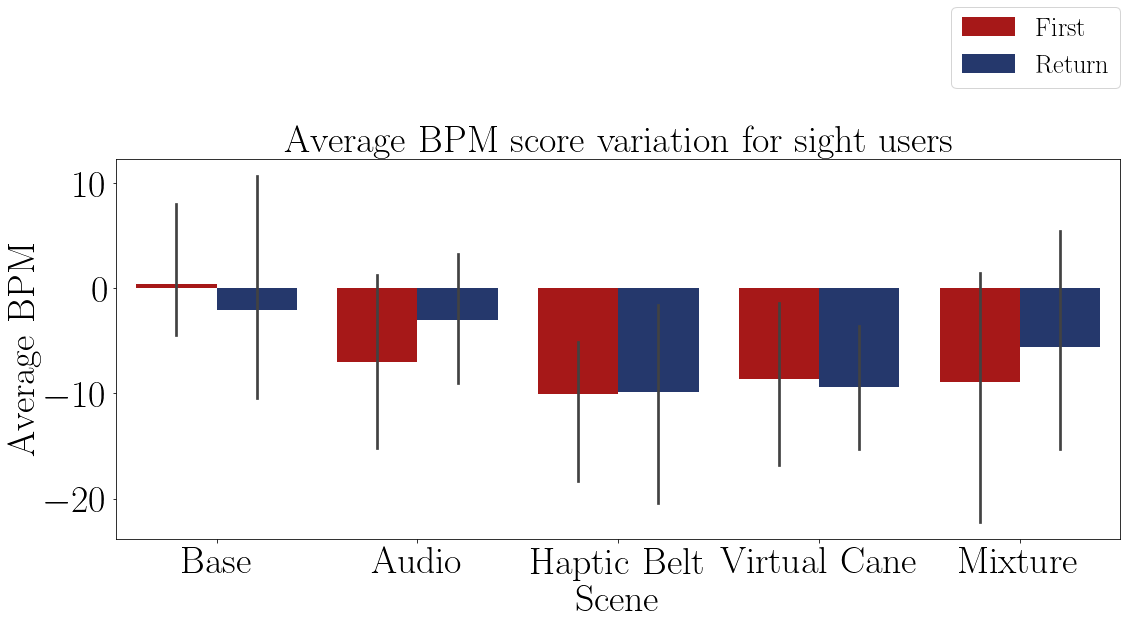
\includegraphics[width = 0.8\linewidth]{Resultados/ECG/Figuras/png/barplot_ecg_bpm_scene_sight.png}
        %\resizebox{0.6\linewidth}{!}{
        %%% Creator: Matplotlib, PGF backend
%%
%% To include the figure in your LaTeX document, write
%%   \input{<filename>.pgf}
%%
%% Make sure the required packages are loaded in your preamble
%%   \usepackage{pgf}
%%
%% Figures using additional raster images can only be included by \input if
%% they are in the same directory as the main LaTeX file. For loading figures
%% from other directories you can use the `import` package
%%   \usepackage{import}
%%
%% and then include the figures with
%%   \import{<path to file>}{<filename>.pgf}
%%
%% Matplotlib used the following preamble
%%   \usepackage{fontspec}
%%
\begingroup%
\makeatletter%
\begin{pgfpicture}%
\pgfpathrectangle{\pgfpointorigin}{\pgfqpoint{15.369508in}{8.690562in}}%
\pgfusepath{use as bounding box, clip}%
\begin{pgfscope}%
\pgfsetbuttcap%
\pgfsetmiterjoin%
\pgfsetlinewidth{0.000000pt}%
\definecolor{currentstroke}{rgb}{1.000000,1.000000,1.000000}%
\pgfsetstrokecolor{currentstroke}%
\pgfsetstrokeopacity{0.000000}%
\pgfsetdash{}{0pt}%
\pgfpathmoveto{\pgfqpoint{0.000000in}{-0.000000in}}%
\pgfpathlineto{\pgfqpoint{15.369508in}{-0.000000in}}%
\pgfpathlineto{\pgfqpoint{15.369508in}{8.690562in}}%
\pgfpathlineto{\pgfqpoint{0.000000in}{8.690562in}}%
\pgfpathclose%
\pgfusepath{}%
\end{pgfscope}%
\begin{pgfscope}%
\pgfsetbuttcap%
\pgfsetmiterjoin%
\definecolor{currentfill}{rgb}{1.000000,1.000000,1.000000}%
\pgfsetfillcolor{currentfill}%
\pgfsetlinewidth{0.000000pt}%
\definecolor{currentstroke}{rgb}{0.000000,0.000000,0.000000}%
\pgfsetstrokecolor{currentstroke}%
\pgfsetstrokeopacity{0.000000}%
\pgfsetdash{}{0pt}%
\pgfpathmoveto{\pgfqpoint{1.319508in}{1.191562in}}%
\pgfpathlineto{\pgfqpoint{15.269508in}{1.191562in}}%
\pgfpathlineto{\pgfqpoint{15.269508in}{6.476562in}}%
\pgfpathlineto{\pgfqpoint{1.319508in}{6.476562in}}%
\pgfpathclose%
\pgfusepath{fill}%
\end{pgfscope}%
\begin{pgfscope}%
\pgfpathrectangle{\pgfqpoint{1.319508in}{1.191562in}}{\pgfqpoint{13.950000in}{5.285000in}}%
\pgfusepath{clip}%
\pgfsetbuttcap%
\pgfsetmiterjoin%
\definecolor{currentfill}{rgb}{0.651961,0.093137,0.093137}%
\pgfsetfillcolor{currentfill}%
\pgfsetlinewidth{0.000000pt}%
\definecolor{currentstroke}{rgb}{0.000000,0.000000,0.000000}%
\pgfsetstrokecolor{currentstroke}%
\pgfsetstrokeopacity{0.000000}%
\pgfsetdash{}{0pt}%
\pgfpathmoveto{\pgfqpoint{1.598508in}{4.680673in}}%
\pgfpathlineto{\pgfqpoint{2.714508in}{4.680673in}}%
\pgfpathlineto{\pgfqpoint{2.714508in}{4.741049in}}%
\pgfpathlineto{\pgfqpoint{1.598508in}{4.741049in}}%
\pgfpathclose%
\pgfusepath{fill}%
\end{pgfscope}%
\begin{pgfscope}%
\pgfpathrectangle{\pgfqpoint{1.319508in}{1.191562in}}{\pgfqpoint{13.950000in}{5.285000in}}%
\pgfusepath{clip}%
\pgfsetbuttcap%
\pgfsetmiterjoin%
\definecolor{currentfill}{rgb}{0.651961,0.093137,0.093137}%
\pgfsetfillcolor{currentfill}%
\pgfsetlinewidth{0.000000pt}%
\definecolor{currentstroke}{rgb}{0.000000,0.000000,0.000000}%
\pgfsetstrokecolor{currentstroke}%
\pgfsetstrokeopacity{0.000000}%
\pgfsetdash{}{0pt}%
\pgfpathmoveto{\pgfqpoint{4.388508in}{4.680673in}}%
\pgfpathlineto{\pgfqpoint{5.504508in}{4.680673in}}%
\pgfpathlineto{\pgfqpoint{5.504508in}{3.662866in}}%
\pgfpathlineto{\pgfqpoint{4.388508in}{3.662866in}}%
\pgfpathclose%
\pgfusepath{fill}%
\end{pgfscope}%
\begin{pgfscope}%
\pgfpathrectangle{\pgfqpoint{1.319508in}{1.191562in}}{\pgfqpoint{13.950000in}{5.285000in}}%
\pgfusepath{clip}%
\pgfsetbuttcap%
\pgfsetmiterjoin%
\definecolor{currentfill}{rgb}{0.651961,0.093137,0.093137}%
\pgfsetfillcolor{currentfill}%
\pgfsetlinewidth{0.000000pt}%
\definecolor{currentstroke}{rgb}{0.000000,0.000000,0.000000}%
\pgfsetstrokecolor{currentstroke}%
\pgfsetstrokeopacity{0.000000}%
\pgfsetdash{}{0pt}%
\pgfpathmoveto{\pgfqpoint{7.178508in}{4.680673in}}%
\pgfpathlineto{\pgfqpoint{8.294508in}{4.680673in}}%
\pgfpathlineto{\pgfqpoint{8.294508in}{3.215289in}}%
\pgfpathlineto{\pgfqpoint{7.178508in}{3.215289in}}%
\pgfpathclose%
\pgfusepath{fill}%
\end{pgfscope}%
\begin{pgfscope}%
\pgfpathrectangle{\pgfqpoint{1.319508in}{1.191562in}}{\pgfqpoint{13.950000in}{5.285000in}}%
\pgfusepath{clip}%
\pgfsetbuttcap%
\pgfsetmiterjoin%
\definecolor{currentfill}{rgb}{0.651961,0.093137,0.093137}%
\pgfsetfillcolor{currentfill}%
\pgfsetlinewidth{0.000000pt}%
\definecolor{currentstroke}{rgb}{0.000000,0.000000,0.000000}%
\pgfsetstrokecolor{currentstroke}%
\pgfsetstrokeopacity{0.000000}%
\pgfsetdash{}{0pt}%
\pgfpathmoveto{\pgfqpoint{9.968508in}{4.680673in}}%
\pgfpathlineto{\pgfqpoint{11.084508in}{4.680673in}}%
\pgfpathlineto{\pgfqpoint{11.084508in}{3.425459in}}%
\pgfpathlineto{\pgfqpoint{9.968508in}{3.425459in}}%
\pgfpathclose%
\pgfusepath{fill}%
\end{pgfscope}%
\begin{pgfscope}%
\pgfpathrectangle{\pgfqpoint{1.319508in}{1.191562in}}{\pgfqpoint{13.950000in}{5.285000in}}%
\pgfusepath{clip}%
\pgfsetbuttcap%
\pgfsetmiterjoin%
\definecolor{currentfill}{rgb}{0.651961,0.093137,0.093137}%
\pgfsetfillcolor{currentfill}%
\pgfsetlinewidth{0.000000pt}%
\definecolor{currentstroke}{rgb}{0.000000,0.000000,0.000000}%
\pgfsetstrokecolor{currentstroke}%
\pgfsetstrokeopacity{0.000000}%
\pgfsetdash{}{0pt}%
\pgfpathmoveto{\pgfqpoint{12.758508in}{4.680673in}}%
\pgfpathlineto{\pgfqpoint{13.874508in}{4.680673in}}%
\pgfpathlineto{\pgfqpoint{13.874508in}{3.378145in}}%
\pgfpathlineto{\pgfqpoint{12.758508in}{3.378145in}}%
\pgfpathclose%
\pgfusepath{fill}%
\end{pgfscope}%
\begin{pgfscope}%
\pgfpathrectangle{\pgfqpoint{1.319508in}{1.191562in}}{\pgfqpoint{13.950000in}{5.285000in}}%
\pgfusepath{clip}%
\pgfsetbuttcap%
\pgfsetmiterjoin%
\definecolor{currentfill}{rgb}{0.144608,0.218137,0.424020}%
\pgfsetfillcolor{currentfill}%
\pgfsetlinewidth{0.000000pt}%
\definecolor{currentstroke}{rgb}{0.000000,0.000000,0.000000}%
\pgfsetstrokecolor{currentstroke}%
\pgfsetstrokeopacity{0.000000}%
\pgfsetdash{}{0pt}%
\pgfpathmoveto{\pgfqpoint{2.714508in}{4.680673in}}%
\pgfpathlineto{\pgfqpoint{3.830508in}{4.680673in}}%
\pgfpathlineto{\pgfqpoint{3.830508in}{4.383066in}}%
\pgfpathlineto{\pgfqpoint{2.714508in}{4.383066in}}%
\pgfpathclose%
\pgfusepath{fill}%
\end{pgfscope}%
\begin{pgfscope}%
\pgfpathrectangle{\pgfqpoint{1.319508in}{1.191562in}}{\pgfqpoint{13.950000in}{5.285000in}}%
\pgfusepath{clip}%
\pgfsetbuttcap%
\pgfsetmiterjoin%
\definecolor{currentfill}{rgb}{0.144608,0.218137,0.424020}%
\pgfsetfillcolor{currentfill}%
\pgfsetlinewidth{0.000000pt}%
\definecolor{currentstroke}{rgb}{0.000000,0.000000,0.000000}%
\pgfsetstrokecolor{currentstroke}%
\pgfsetstrokeopacity{0.000000}%
\pgfsetdash{}{0pt}%
\pgfpathmoveto{\pgfqpoint{5.504508in}{4.680673in}}%
\pgfpathlineto{\pgfqpoint{6.620508in}{4.680673in}}%
\pgfpathlineto{\pgfqpoint{6.620508in}{4.244260in}}%
\pgfpathlineto{\pgfqpoint{5.504508in}{4.244260in}}%
\pgfpathclose%
\pgfusepath{fill}%
\end{pgfscope}%
\begin{pgfscope}%
\pgfpathrectangle{\pgfqpoint{1.319508in}{1.191562in}}{\pgfqpoint{13.950000in}{5.285000in}}%
\pgfusepath{clip}%
\pgfsetbuttcap%
\pgfsetmiterjoin%
\definecolor{currentfill}{rgb}{0.144608,0.218137,0.424020}%
\pgfsetfillcolor{currentfill}%
\pgfsetlinewidth{0.000000pt}%
\definecolor{currentstroke}{rgb}{0.000000,0.000000,0.000000}%
\pgfsetstrokecolor{currentstroke}%
\pgfsetstrokeopacity{0.000000}%
\pgfsetdash{}{0pt}%
\pgfpathmoveto{\pgfqpoint{8.294508in}{4.680673in}}%
\pgfpathlineto{\pgfqpoint{9.410508in}{4.680673in}}%
\pgfpathlineto{\pgfqpoint{9.410508in}{3.234717in}}%
\pgfpathlineto{\pgfqpoint{8.294508in}{3.234717in}}%
\pgfpathclose%
\pgfusepath{fill}%
\end{pgfscope}%
\begin{pgfscope}%
\pgfpathrectangle{\pgfqpoint{1.319508in}{1.191562in}}{\pgfqpoint{13.950000in}{5.285000in}}%
\pgfusepath{clip}%
\pgfsetbuttcap%
\pgfsetmiterjoin%
\definecolor{currentfill}{rgb}{0.144608,0.218137,0.424020}%
\pgfsetfillcolor{currentfill}%
\pgfsetlinewidth{0.000000pt}%
\definecolor{currentstroke}{rgb}{0.000000,0.000000,0.000000}%
\pgfsetstrokecolor{currentstroke}%
\pgfsetstrokeopacity{0.000000}%
\pgfsetdash{}{0pt}%
\pgfpathmoveto{\pgfqpoint{11.084508in}{4.680673in}}%
\pgfpathlineto{\pgfqpoint{12.200508in}{4.680673in}}%
\pgfpathlineto{\pgfqpoint{12.200508in}{3.302703in}}%
\pgfpathlineto{\pgfqpoint{11.084508in}{3.302703in}}%
\pgfpathclose%
\pgfusepath{fill}%
\end{pgfscope}%
\begin{pgfscope}%
\pgfpathrectangle{\pgfqpoint{1.319508in}{1.191562in}}{\pgfqpoint{13.950000in}{5.285000in}}%
\pgfusepath{clip}%
\pgfsetbuttcap%
\pgfsetmiterjoin%
\definecolor{currentfill}{rgb}{0.144608,0.218137,0.424020}%
\pgfsetfillcolor{currentfill}%
\pgfsetlinewidth{0.000000pt}%
\definecolor{currentstroke}{rgb}{0.000000,0.000000,0.000000}%
\pgfsetstrokecolor{currentstroke}%
\pgfsetstrokeopacity{0.000000}%
\pgfsetdash{}{0pt}%
\pgfpathmoveto{\pgfqpoint{13.874508in}{4.680673in}}%
\pgfpathlineto{\pgfqpoint{14.990508in}{4.680673in}}%
\pgfpathlineto{\pgfqpoint{14.990508in}{3.868838in}}%
\pgfpathlineto{\pgfqpoint{13.874508in}{3.868838in}}%
\pgfpathclose%
\pgfusepath{fill}%
\end{pgfscope}%
\begin{pgfscope}%
\pgfsetbuttcap%
\pgfsetroundjoin%
\definecolor{currentfill}{rgb}{0.000000,0.000000,0.000000}%
\pgfsetfillcolor{currentfill}%
\pgfsetlinewidth{0.803000pt}%
\definecolor{currentstroke}{rgb}{0.000000,0.000000,0.000000}%
\pgfsetstrokecolor{currentstroke}%
\pgfsetdash{}{0pt}%
\pgfsys@defobject{currentmarker}{\pgfqpoint{0.000000in}{-0.048611in}}{\pgfqpoint{0.000000in}{0.000000in}}{%
\pgfpathmoveto{\pgfqpoint{0.000000in}{0.000000in}}%
\pgfpathlineto{\pgfqpoint{0.000000in}{-0.048611in}}%
\pgfusepath{stroke,fill}%
}%
\begin{pgfscope}%
\pgfsys@transformshift{2.714508in}{1.191562in}%
\pgfsys@useobject{currentmarker}{}%
\end{pgfscope}%
\end{pgfscope}%
\begin{pgfscope}%
\definecolor{textcolor}{rgb}{0.000000,0.000000,0.000000}%
\pgfsetstrokecolor{textcolor}%
\pgfsetfillcolor{textcolor}%
\pgftext[x=2.714508in,y=1.094339in,,top]{\color{textcolor}\rmfamily\fontsize{38.016000}{45.619200}\selectfont Base}%
\end{pgfscope}%
\begin{pgfscope}%
\pgfsetbuttcap%
\pgfsetroundjoin%
\definecolor{currentfill}{rgb}{0.000000,0.000000,0.000000}%
\pgfsetfillcolor{currentfill}%
\pgfsetlinewidth{0.803000pt}%
\definecolor{currentstroke}{rgb}{0.000000,0.000000,0.000000}%
\pgfsetstrokecolor{currentstroke}%
\pgfsetdash{}{0pt}%
\pgfsys@defobject{currentmarker}{\pgfqpoint{0.000000in}{-0.048611in}}{\pgfqpoint{0.000000in}{0.000000in}}{%
\pgfpathmoveto{\pgfqpoint{0.000000in}{0.000000in}}%
\pgfpathlineto{\pgfqpoint{0.000000in}{-0.048611in}}%
\pgfusepath{stroke,fill}%
}%
\begin{pgfscope}%
\pgfsys@transformshift{5.504508in}{1.191562in}%
\pgfsys@useobject{currentmarker}{}%
\end{pgfscope}%
\end{pgfscope}%
\begin{pgfscope}%
\definecolor{textcolor}{rgb}{0.000000,0.000000,0.000000}%
\pgfsetstrokecolor{textcolor}%
\pgfsetfillcolor{textcolor}%
\pgftext[x=5.504508in,y=1.094339in,,top]{\color{textcolor}\rmfamily\fontsize{38.016000}{45.619200}\selectfont Audio}%
\end{pgfscope}%
\begin{pgfscope}%
\pgfsetbuttcap%
\pgfsetroundjoin%
\definecolor{currentfill}{rgb}{0.000000,0.000000,0.000000}%
\pgfsetfillcolor{currentfill}%
\pgfsetlinewidth{0.803000pt}%
\definecolor{currentstroke}{rgb}{0.000000,0.000000,0.000000}%
\pgfsetstrokecolor{currentstroke}%
\pgfsetdash{}{0pt}%
\pgfsys@defobject{currentmarker}{\pgfqpoint{0.000000in}{-0.048611in}}{\pgfqpoint{0.000000in}{0.000000in}}{%
\pgfpathmoveto{\pgfqpoint{0.000000in}{0.000000in}}%
\pgfpathlineto{\pgfqpoint{0.000000in}{-0.048611in}}%
\pgfusepath{stroke,fill}%
}%
\begin{pgfscope}%
\pgfsys@transformshift{8.294508in}{1.191562in}%
\pgfsys@useobject{currentmarker}{}%
\end{pgfscope}%
\end{pgfscope}%
\begin{pgfscope}%
\definecolor{textcolor}{rgb}{0.000000,0.000000,0.000000}%
\pgfsetstrokecolor{textcolor}%
\pgfsetfillcolor{textcolor}%
\pgftext[x=8.294508in,y=1.094339in,,top]{\color{textcolor}\rmfamily\fontsize{38.016000}{45.619200}\selectfont Haptic Belt}%
\end{pgfscope}%
\begin{pgfscope}%
\pgfsetbuttcap%
\pgfsetroundjoin%
\definecolor{currentfill}{rgb}{0.000000,0.000000,0.000000}%
\pgfsetfillcolor{currentfill}%
\pgfsetlinewidth{0.803000pt}%
\definecolor{currentstroke}{rgb}{0.000000,0.000000,0.000000}%
\pgfsetstrokecolor{currentstroke}%
\pgfsetdash{}{0pt}%
\pgfsys@defobject{currentmarker}{\pgfqpoint{0.000000in}{-0.048611in}}{\pgfqpoint{0.000000in}{0.000000in}}{%
\pgfpathmoveto{\pgfqpoint{0.000000in}{0.000000in}}%
\pgfpathlineto{\pgfqpoint{0.000000in}{-0.048611in}}%
\pgfusepath{stroke,fill}%
}%
\begin{pgfscope}%
\pgfsys@transformshift{11.084508in}{1.191562in}%
\pgfsys@useobject{currentmarker}{}%
\end{pgfscope}%
\end{pgfscope}%
\begin{pgfscope}%
\definecolor{textcolor}{rgb}{0.000000,0.000000,0.000000}%
\pgfsetstrokecolor{textcolor}%
\pgfsetfillcolor{textcolor}%
\pgftext[x=11.084508in,y=1.094339in,,top]{\color{textcolor}\rmfamily\fontsize{38.016000}{45.619200}\selectfont Virtual Cane}%
\end{pgfscope}%
\begin{pgfscope}%
\pgfsetbuttcap%
\pgfsetroundjoin%
\definecolor{currentfill}{rgb}{0.000000,0.000000,0.000000}%
\pgfsetfillcolor{currentfill}%
\pgfsetlinewidth{0.803000pt}%
\definecolor{currentstroke}{rgb}{0.000000,0.000000,0.000000}%
\pgfsetstrokecolor{currentstroke}%
\pgfsetdash{}{0pt}%
\pgfsys@defobject{currentmarker}{\pgfqpoint{0.000000in}{-0.048611in}}{\pgfqpoint{0.000000in}{0.000000in}}{%
\pgfpathmoveto{\pgfqpoint{0.000000in}{0.000000in}}%
\pgfpathlineto{\pgfqpoint{0.000000in}{-0.048611in}}%
\pgfusepath{stroke,fill}%
}%
\begin{pgfscope}%
\pgfsys@transformshift{13.874508in}{1.191562in}%
\pgfsys@useobject{currentmarker}{}%
\end{pgfscope}%
\end{pgfscope}%
\begin{pgfscope}%
\definecolor{textcolor}{rgb}{0.000000,0.000000,0.000000}%
\pgfsetstrokecolor{textcolor}%
\pgfsetfillcolor{textcolor}%
\pgftext[x=13.874508in,y=1.094339in,,top]{\color{textcolor}\rmfamily\fontsize{38.016000}{45.619200}\selectfont Mixture}%
\end{pgfscope}%
\begin{pgfscope}%
\definecolor{textcolor}{rgb}{0.000000,0.000000,0.000000}%
\pgfsetstrokecolor{textcolor}%
\pgfsetfillcolor{textcolor}%
\pgftext[x=8.294508in,y=0.569392in,,top]{\color{textcolor}\rmfamily\fontsize{38.016000}{45.619200}\selectfont Scene}%
\end{pgfscope}%
\begin{pgfscope}%
\pgfsetbuttcap%
\pgfsetroundjoin%
\definecolor{currentfill}{rgb}{0.000000,0.000000,0.000000}%
\pgfsetfillcolor{currentfill}%
\pgfsetlinewidth{0.803000pt}%
\definecolor{currentstroke}{rgb}{0.000000,0.000000,0.000000}%
\pgfsetstrokecolor{currentstroke}%
\pgfsetdash{}{0pt}%
\pgfsys@defobject{currentmarker}{\pgfqpoint{-0.048611in}{0.000000in}}{\pgfqpoint{-0.000000in}{0.000000in}}{%
\pgfpathmoveto{\pgfqpoint{-0.000000in}{0.000000in}}%
\pgfpathlineto{\pgfqpoint{-0.048611in}{0.000000in}}%
\pgfusepath{stroke,fill}%
}%
\begin{pgfscope}%
\pgfsys@transformshift{1.319508in}{1.759960in}%
\pgfsys@useobject{currentmarker}{}%
\end{pgfscope}%
\end{pgfscope}%
\begin{pgfscope}%
\definecolor{textcolor}{rgb}{0.000000,0.000000,0.000000}%
\pgfsetstrokecolor{textcolor}%
\pgfsetfillcolor{textcolor}%
\pgftext[x=0.636563in, y=1.576744in, left, base]{\color{textcolor}\rmfamily\fontsize{38.016000}{45.619200}\selectfont \(\displaystyle {\ensuremath{-}20}\)}%
\end{pgfscope}%
\begin{pgfscope}%
\pgfsetbuttcap%
\pgfsetroundjoin%
\definecolor{currentfill}{rgb}{0.000000,0.000000,0.000000}%
\pgfsetfillcolor{currentfill}%
\pgfsetlinewidth{0.803000pt}%
\definecolor{currentstroke}{rgb}{0.000000,0.000000,0.000000}%
\pgfsetstrokecolor{currentstroke}%
\pgfsetdash{}{0pt}%
\pgfsys@defobject{currentmarker}{\pgfqpoint{-0.048611in}{0.000000in}}{\pgfqpoint{-0.000000in}{0.000000in}}{%
\pgfpathmoveto{\pgfqpoint{-0.000000in}{0.000000in}}%
\pgfpathlineto{\pgfqpoint{-0.048611in}{0.000000in}}%
\pgfusepath{stroke,fill}%
}%
\begin{pgfscope}%
\pgfsys@transformshift{1.319508in}{3.220316in}%
\pgfsys@useobject{currentmarker}{}%
\end{pgfscope}%
\end{pgfscope}%
\begin{pgfscope}%
\definecolor{textcolor}{rgb}{0.000000,0.000000,0.000000}%
\pgfsetstrokecolor{textcolor}%
\pgfsetfillcolor{textcolor}%
\pgftext[x=0.636563in, y=3.037100in, left, base]{\color{textcolor}\rmfamily\fontsize{38.016000}{45.619200}\selectfont \(\displaystyle {\ensuremath{-}10}\)}%
\end{pgfscope}%
\begin{pgfscope}%
\pgfsetbuttcap%
\pgfsetroundjoin%
\definecolor{currentfill}{rgb}{0.000000,0.000000,0.000000}%
\pgfsetfillcolor{currentfill}%
\pgfsetlinewidth{0.803000pt}%
\definecolor{currentstroke}{rgb}{0.000000,0.000000,0.000000}%
\pgfsetstrokecolor{currentstroke}%
\pgfsetdash{}{0pt}%
\pgfsys@defobject{currentmarker}{\pgfqpoint{-0.048611in}{0.000000in}}{\pgfqpoint{-0.000000in}{0.000000in}}{%
\pgfpathmoveto{\pgfqpoint{-0.000000in}{0.000000in}}%
\pgfpathlineto{\pgfqpoint{-0.048611in}{0.000000in}}%
\pgfusepath{stroke,fill}%
}%
\begin{pgfscope}%
\pgfsys@transformshift{1.319508in}{4.680673in}%
\pgfsys@useobject{currentmarker}{}%
\end{pgfscope}%
\end{pgfscope}%
\begin{pgfscope}%
\definecolor{textcolor}{rgb}{0.000000,0.000000,0.000000}%
\pgfsetstrokecolor{textcolor}%
\pgfsetfillcolor{textcolor}%
\pgftext[x=1.063808in, y=4.497457in, left, base]{\color{textcolor}\rmfamily\fontsize{38.016000}{45.619200}\selectfont \(\displaystyle {0}\)}%
\end{pgfscope}%
\begin{pgfscope}%
\pgfsetbuttcap%
\pgfsetroundjoin%
\definecolor{currentfill}{rgb}{0.000000,0.000000,0.000000}%
\pgfsetfillcolor{currentfill}%
\pgfsetlinewidth{0.803000pt}%
\definecolor{currentstroke}{rgb}{0.000000,0.000000,0.000000}%
\pgfsetstrokecolor{currentstroke}%
\pgfsetdash{}{0pt}%
\pgfsys@defobject{currentmarker}{\pgfqpoint{-0.048611in}{0.000000in}}{\pgfqpoint{-0.000000in}{0.000000in}}{%
\pgfpathmoveto{\pgfqpoint{-0.000000in}{0.000000in}}%
\pgfpathlineto{\pgfqpoint{-0.048611in}{0.000000in}}%
\pgfusepath{stroke,fill}%
}%
\begin{pgfscope}%
\pgfsys@transformshift{1.319508in}{6.141029in}%
\pgfsys@useobject{currentmarker}{}%
\end{pgfscope}%
\end{pgfscope}%
\begin{pgfscope}%
\definecolor{textcolor}{rgb}{0.000000,0.000000,0.000000}%
\pgfsetstrokecolor{textcolor}%
\pgfsetfillcolor{textcolor}%
\pgftext[x=0.905330in, y=5.957813in, left, base]{\color{textcolor}\rmfamily\fontsize{38.016000}{45.619200}\selectfont \(\displaystyle {10}\)}%
\end{pgfscope}%
\begin{pgfscope}%
\definecolor{textcolor}{rgb}{0.000000,0.000000,0.000000}%
\pgfsetstrokecolor{textcolor}%
\pgfsetfillcolor{textcolor}%
\pgftext[x=0.581008in,y=3.834062in,,bottom,rotate=90.000000]{\color{textcolor}\rmfamily\fontsize{38.016000}{45.619200}\selectfont Average BPM}%
\end{pgfscope}%
\begin{pgfscope}%
\pgfpathrectangle{\pgfqpoint{1.319508in}{1.191562in}}{\pgfqpoint{13.950000in}{5.285000in}}%
\pgfusepath{clip}%
\pgfsetrectcap%
\pgfsetroundjoin%
\pgfsetlinewidth{2.710125pt}%
\definecolor{currentstroke}{rgb}{0.260000,0.260000,0.260000}%
\pgfsetstrokecolor{currentstroke}%
\pgfsetdash{}{0pt}%
\pgfpathmoveto{\pgfqpoint{2.156508in}{3.970565in}}%
\pgfpathlineto{\pgfqpoint{2.156508in}{5.766272in}}%
\pgfusepath{stroke}%
\end{pgfscope}%
\begin{pgfscope}%
\pgfpathrectangle{\pgfqpoint{1.319508in}{1.191562in}}{\pgfqpoint{13.950000in}{5.285000in}}%
\pgfusepath{clip}%
\pgfsetrectcap%
\pgfsetroundjoin%
\pgfsetlinewidth{2.710125pt}%
\definecolor{currentstroke}{rgb}{0.260000,0.260000,0.260000}%
\pgfsetstrokecolor{currentstroke}%
\pgfsetdash{}{0pt}%
\pgfpathmoveto{\pgfqpoint{4.946508in}{2.464955in}}%
\pgfpathlineto{\pgfqpoint{4.946508in}{4.860777in}}%
\pgfusepath{stroke}%
\end{pgfscope}%
\begin{pgfscope}%
\pgfpathrectangle{\pgfqpoint{1.319508in}{1.191562in}}{\pgfqpoint{13.950000in}{5.285000in}}%
\pgfusepath{clip}%
\pgfsetrectcap%
\pgfsetroundjoin%
\pgfsetlinewidth{2.710125pt}%
\definecolor{currentstroke}{rgb}{0.260000,0.260000,0.260000}%
\pgfsetstrokecolor{currentstroke}%
\pgfsetdash{}{0pt}%
\pgfpathmoveto{\pgfqpoint{7.736508in}{1.998402in}}%
\pgfpathlineto{\pgfqpoint{7.736508in}{3.936033in}}%
\pgfusepath{stroke}%
\end{pgfscope}%
\begin{pgfscope}%
\pgfpathrectangle{\pgfqpoint{1.319508in}{1.191562in}}{\pgfqpoint{13.950000in}{5.285000in}}%
\pgfusepath{clip}%
\pgfsetrectcap%
\pgfsetroundjoin%
\pgfsetlinewidth{2.710125pt}%
\definecolor{currentstroke}{rgb}{0.260000,0.260000,0.260000}%
\pgfsetstrokecolor{currentstroke}%
\pgfsetdash{}{0pt}%
\pgfpathmoveto{\pgfqpoint{10.526508in}{2.220154in}}%
\pgfpathlineto{\pgfqpoint{10.526508in}{4.478297in}}%
\pgfusepath{stroke}%
\end{pgfscope}%
\begin{pgfscope}%
\pgfpathrectangle{\pgfqpoint{1.319508in}{1.191562in}}{\pgfqpoint{13.950000in}{5.285000in}}%
\pgfusepath{clip}%
\pgfsetrectcap%
\pgfsetroundjoin%
\pgfsetlinewidth{2.710125pt}%
\definecolor{currentstroke}{rgb}{0.260000,0.260000,0.260000}%
\pgfsetstrokecolor{currentstroke}%
\pgfsetdash{}{0pt}%
\pgfpathmoveto{\pgfqpoint{13.316508in}{1.431789in}}%
\pgfpathlineto{\pgfqpoint{13.316508in}{4.887907in}}%
\pgfusepath{stroke}%
\end{pgfscope}%
\begin{pgfscope}%
\pgfpathrectangle{\pgfqpoint{1.319508in}{1.191562in}}{\pgfqpoint{13.950000in}{5.285000in}}%
\pgfusepath{clip}%
\pgfsetrectcap%
\pgfsetroundjoin%
\pgfsetlinewidth{2.710125pt}%
\definecolor{currentstroke}{rgb}{0.260000,0.260000,0.260000}%
\pgfsetstrokecolor{currentstroke}%
\pgfsetdash{}{0pt}%
\pgfpathmoveto{\pgfqpoint{3.272508in}{3.162266in}}%
\pgfpathlineto{\pgfqpoint{3.272508in}{6.236334in}}%
\pgfusepath{stroke}%
\end{pgfscope}%
\begin{pgfscope}%
\pgfpathrectangle{\pgfqpoint{1.319508in}{1.191562in}}{\pgfqpoint{13.950000in}{5.285000in}}%
\pgfusepath{clip}%
\pgfsetrectcap%
\pgfsetroundjoin%
\pgfsetlinewidth{2.710125pt}%
\definecolor{currentstroke}{rgb}{0.260000,0.260000,0.260000}%
\pgfsetstrokecolor{currentstroke}%
\pgfsetdash{}{0pt}%
\pgfpathmoveto{\pgfqpoint{6.062508in}{3.502466in}}%
\pgfpathlineto{\pgfqpoint{6.062508in}{5.158738in}}%
\pgfusepath{stroke}%
\end{pgfscope}%
\begin{pgfscope}%
\pgfpathrectangle{\pgfqpoint{1.319508in}{1.191562in}}{\pgfqpoint{13.950000in}{5.285000in}}%
\pgfusepath{clip}%
\pgfsetrectcap%
\pgfsetroundjoin%
\pgfsetlinewidth{2.710125pt}%
\definecolor{currentstroke}{rgb}{0.260000,0.260000,0.260000}%
\pgfsetstrokecolor{currentstroke}%
\pgfsetdash{}{0pt}%
\pgfpathmoveto{\pgfqpoint{8.852508in}{1.700683in}}%
\pgfpathlineto{\pgfqpoint{8.852508in}{4.445199in}}%
\pgfusepath{stroke}%
\end{pgfscope}%
\begin{pgfscope}%
\pgfpathrectangle{\pgfqpoint{1.319508in}{1.191562in}}{\pgfqpoint{13.950000in}{5.285000in}}%
\pgfusepath{clip}%
\pgfsetrectcap%
\pgfsetroundjoin%
\pgfsetlinewidth{2.710125pt}%
\definecolor{currentstroke}{rgb}{0.260000,0.260000,0.260000}%
\pgfsetstrokecolor{currentstroke}%
\pgfsetdash{}{0pt}%
\pgfpathmoveto{\pgfqpoint{11.642508in}{2.443751in}}%
\pgfpathlineto{\pgfqpoint{11.642508in}{4.161655in}}%
\pgfusepath{stroke}%
\end{pgfscope}%
\begin{pgfscope}%
\pgfpathrectangle{\pgfqpoint{1.319508in}{1.191562in}}{\pgfqpoint{13.950000in}{5.285000in}}%
\pgfusepath{clip}%
\pgfsetrectcap%
\pgfsetroundjoin%
\pgfsetlinewidth{2.710125pt}%
\definecolor{currentstroke}{rgb}{0.260000,0.260000,0.260000}%
\pgfsetstrokecolor{currentstroke}%
\pgfsetdash{}{0pt}%
\pgfpathmoveto{\pgfqpoint{14.432508in}{2.359990in}}%
\pgfpathlineto{\pgfqpoint{14.432508in}{5.480374in}}%
\pgfusepath{stroke}%
\end{pgfscope}%
\begin{pgfscope}%
\pgfsetrectcap%
\pgfsetmiterjoin%
\pgfsetlinewidth{0.803000pt}%
\definecolor{currentstroke}{rgb}{0.000000,0.000000,0.000000}%
\pgfsetstrokecolor{currentstroke}%
\pgfsetdash{}{0pt}%
\pgfpathmoveto{\pgfqpoint{1.319508in}{1.191562in}}%
\pgfpathlineto{\pgfqpoint{1.319508in}{6.476562in}}%
\pgfusepath{stroke}%
\end{pgfscope}%
\begin{pgfscope}%
\pgfsetrectcap%
\pgfsetmiterjoin%
\pgfsetlinewidth{0.803000pt}%
\definecolor{currentstroke}{rgb}{0.000000,0.000000,0.000000}%
\pgfsetstrokecolor{currentstroke}%
\pgfsetdash{}{0pt}%
\pgfpathmoveto{\pgfqpoint{15.269508in}{1.191562in}}%
\pgfpathlineto{\pgfqpoint{15.269508in}{6.476562in}}%
\pgfusepath{stroke}%
\end{pgfscope}%
\begin{pgfscope}%
\pgfsetrectcap%
\pgfsetmiterjoin%
\pgfsetlinewidth{0.803000pt}%
\definecolor{currentstroke}{rgb}{0.000000,0.000000,0.000000}%
\pgfsetstrokecolor{currentstroke}%
\pgfsetdash{}{0pt}%
\pgfpathmoveto{\pgfqpoint{1.319508in}{1.191562in}}%
\pgfpathlineto{\pgfqpoint{15.269508in}{1.191562in}}%
\pgfusepath{stroke}%
\end{pgfscope}%
\begin{pgfscope}%
\pgfsetrectcap%
\pgfsetmiterjoin%
\pgfsetlinewidth{0.803000pt}%
\definecolor{currentstroke}{rgb}{0.000000,0.000000,0.000000}%
\pgfsetstrokecolor{currentstroke}%
\pgfsetdash{}{0pt}%
\pgfpathmoveto{\pgfqpoint{1.319508in}{6.476562in}}%
\pgfpathlineto{\pgfqpoint{15.269508in}{6.476562in}}%
\pgfusepath{stroke}%
\end{pgfscope}%
\begin{pgfscope}%
\definecolor{textcolor}{rgb}{0.000000,0.000000,0.000000}%
\pgfsetstrokecolor{textcolor}%
\pgfsetfillcolor{textcolor}%
\pgftext[x=8.294508in,y=6.584273in,,base]{\color{textcolor}\rmfamily\fontsize{38.016000}{45.619200}\selectfont Average BPM score variation for sight users}%
\end{pgfscope}%
\begin{pgfscope}%
\pgfsetbuttcap%
\pgfsetmiterjoin%
\definecolor{currentfill}{rgb}{1.000000,1.000000,1.000000}%
\pgfsetfillcolor{currentfill}%
\pgfsetfillopacity{0.800000}%
\pgfsetlinewidth{1.003750pt}%
\definecolor{currentstroke}{rgb}{0.800000,0.800000,0.800000}%
\pgfsetstrokecolor{currentstroke}%
\pgfsetstrokeopacity{0.800000}%
\pgfsetdash{}{0pt}%
\pgfpathmoveto{\pgfqpoint{12.990308in}{7.457562in}}%
\pgfpathlineto{\pgfqpoint{15.196175in}{7.457562in}}%
\pgfpathquadraticcurveto{\pgfqpoint{15.269508in}{7.457562in}}{\pgfqpoint{15.269508in}{7.530896in}}%
\pgfpathlineto{\pgfqpoint{15.269508in}{8.517228in}}%
\pgfpathquadraticcurveto{\pgfqpoint{15.269508in}{8.590562in}}{\pgfqpoint{15.196175in}{8.590562in}}%
\pgfpathlineto{\pgfqpoint{12.990308in}{8.590562in}}%
\pgfpathquadraticcurveto{\pgfqpoint{12.916975in}{8.590562in}}{\pgfqpoint{12.916975in}{8.517228in}}%
\pgfpathlineto{\pgfqpoint{12.916975in}{7.530896in}}%
\pgfpathquadraticcurveto{\pgfqpoint{12.916975in}{7.457562in}}{\pgfqpoint{12.990308in}{7.457562in}}%
\pgfpathclose%
\pgfusepath{stroke,fill}%
\end{pgfscope}%
\begin{pgfscope}%
\pgfsetbuttcap%
\pgfsetmiterjoin%
\definecolor{currentfill}{rgb}{0.651961,0.093137,0.093137}%
\pgfsetfillcolor{currentfill}%
\pgfsetlinewidth{0.000000pt}%
\definecolor{currentstroke}{rgb}{0.000000,0.000000,0.000000}%
\pgfsetstrokecolor{currentstroke}%
\pgfsetstrokeopacity{0.000000}%
\pgfsetdash{}{0pt}%
\pgfpathmoveto{\pgfqpoint{13.063642in}{8.187228in}}%
\pgfpathlineto{\pgfqpoint{13.796975in}{8.187228in}}%
\pgfpathlineto{\pgfqpoint{13.796975in}{8.443895in}}%
\pgfpathlineto{\pgfqpoint{13.063642in}{8.443895in}}%
\pgfpathclose%
\pgfusepath{fill}%
\end{pgfscope}%
\begin{pgfscope}%
\definecolor{textcolor}{rgb}{0.000000,0.000000,0.000000}%
\pgfsetstrokecolor{textcolor}%
\pgfsetfillcolor{textcolor}%
\pgftext[x=14.090308in,y=8.187228in,left,base]{\color{textcolor}\rmfamily\fontsize{26.400000}{31.680000}\selectfont First}%
\end{pgfscope}%
\begin{pgfscope}%
\pgfsetbuttcap%
\pgfsetmiterjoin%
\definecolor{currentfill}{rgb}{0.144608,0.218137,0.424020}%
\pgfsetfillcolor{currentfill}%
\pgfsetlinewidth{0.000000pt}%
\definecolor{currentstroke}{rgb}{0.000000,0.000000,0.000000}%
\pgfsetstrokecolor{currentstroke}%
\pgfsetstrokeopacity{0.000000}%
\pgfsetdash{}{0pt}%
\pgfpathmoveto{\pgfqpoint{13.063642in}{7.675729in}}%
\pgfpathlineto{\pgfqpoint{13.796975in}{7.675729in}}%
\pgfpathlineto{\pgfqpoint{13.796975in}{7.932395in}}%
\pgfpathlineto{\pgfqpoint{13.063642in}{7.932395in}}%
\pgfpathclose%
\pgfusepath{fill}%
\end{pgfscope}%
\begin{pgfscope}%
\definecolor{textcolor}{rgb}{0.000000,0.000000,0.000000}%
\pgfsetstrokecolor{textcolor}%
\pgfsetfillcolor{textcolor}%
\pgftext[x=14.090308in,y=7.675729in,left,base]{\color{textcolor}\rmfamily\fontsize{26.400000}{31.680000}\selectfont Return}%
\end{pgfscope}%
\end{pgfpicture}%
\makeatother%
\endgroup%
    
        %}
        \caption{Bar plot of the average heart rate of the sighted participants on each method.}
        \label{fig:barplot_ecg_bpm_scene_sight}
    \end{minipage}
\end{figure}


The Table \ref{tab:ecg_bpm_var_etapa} show the the average Sagat score between the rounds of each participant and the Figure \ref{fig:boxplot_sagat_scene} these data is plotted. It is possible only to assume that some methods causes differente Sagat scores than other, but both groups performed rather similarly.


\begin{table}[!htb]
\centering
\caption{ECG average BPM variation between rounds.}
\label{tab:ecg_bpm_var_etapa}
\begin{tabular}{lrrrrrl}
\toprule
{} &    Base &   Audio & \begin{tabular}[c]{@{}l@{}}Haptic\\ Belt\end{tabular} & \begin{tabular}[c]{@{}l@{}}Virtual\\ Cane\end{tabular} & Mixture & \begin{tabular}[c]{@{}l@{}}Visual\\ Condition\end{tabular} \\
Participant &         &         &                                                       &                                                        &         &                                                            \\
\midrule
001         &  -5.2\% &   2.7\% &                                                -2.9\% &                                                  3.0\% &  12.7\% &                                                      Sight \\
001C        &  -6.2\% &  -3.5\% &                                                -6.9\% &                                                  8.7\% &   3.7\% &                                                      Blind \\
002C        &   7.7\% &  23.0\% &                                                21.0\% &                                                 21.0\% &  11.5\% &                                                      Blind \\
003         &  -7.6\% &  14.6\% &                                                -0.8\% &                                                 -4.8\% &   0.3\% &                                                      Sight \\
003C        &  -1.5\% &  -3.5\% &                                                -1.8\% &                                                 -0.8\% &   0.6\% &                                                      Blind \\
004         &   5.3\% &   3.9\% &                                                 5.1\% &                                                 -2.1\% &   5.9\% &                                                      Sight \\
004C        &  -0.5\% &   1.7\% &                                                 0.4\% &                                                  1.0\% &  -9.0\% &                                                      Blind \\
005         &  -3.6\% &  -2.5\% &                                                -1.4\% &                                                  0.8\% &  -2.4\% &                                                      Sight \\
\bottomrule
\end{tabular}
\end{table}



The Figure \ref{fig:boxplot_ecg_bpm_scene} shows a comparison between both groups

\begin{figure}[!htb]
    \centering
    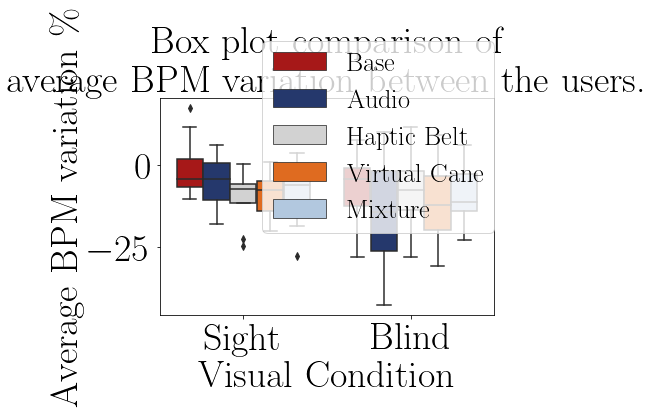
\includegraphics[width = 0.5\linewidth]{Resultados/ECG/Figuras/png/boxplot_ecg_bpm_scene.png}
    %\resizebox{0.6\linewidth}{!}{
    %%% Creator: Matplotlib, PGF backend
%%
%% To include the figure in your LaTeX document, write
%%   \input{<filename>.pgf}
%%
%% Make sure the required packages are loaded in your preamble
%%   \usepackage{pgf}
%%
%% and, on pdftex
%%   \usepackage[utf8]{inputenc}\DeclareUnicodeCharacter{2212}{-}
%%
%% or, on luatex and xetex
%%   \usepackage{unicode-math}
%%
%% Figures using additional raster images can only be included by \input if
%% they are in the same directory as the main LaTeX file. For loading figures
%% from other directories you can use the `import` package
%%   \usepackage{import}
%%
%% and then include the figures with
%%   \import{<path to file>}{<filename>.pgf}
%%
%% Matplotlib used the following preamble
%%   \usepackage{url}
%%   \usepackage{unicode-math}
%%   \setmainfont{DejaVu Serif}
%%   \usepackage{fontspec}
%%
\begingroup%
\makeatletter%
\begin{pgfpicture}%
\pgfpathrectangle{\pgfpointorigin}{\pgfqpoint{12.692598in}{14.528848in}}%
\pgfusepath{use as bounding box, clip}%
\begin{pgfscope}%
\pgfsetbuttcap%
\pgfsetmiterjoin%
\pgfsetlinewidth{0.000000pt}%
\definecolor{currentstroke}{rgb}{1.000000,1.000000,1.000000}%
\pgfsetstrokecolor{currentstroke}%
\pgfsetstrokeopacity{0.000000}%
\pgfsetdash{}{0pt}%
\pgfpathmoveto{\pgfqpoint{0.000000in}{0.000000in}}%
\pgfpathlineto{\pgfqpoint{12.692598in}{0.000000in}}%
\pgfpathlineto{\pgfqpoint{12.692598in}{14.528848in}}%
\pgfpathlineto{\pgfqpoint{0.000000in}{14.528848in}}%
\pgfpathclose%
\pgfusepath{}%
\end{pgfscope}%
\begin{pgfscope}%
\pgfsetbuttcap%
\pgfsetmiterjoin%
\definecolor{currentfill}{rgb}{1.000000,1.000000,1.000000}%
\pgfsetfillcolor{currentfill}%
\pgfsetlinewidth{0.000000pt}%
\definecolor{currentstroke}{rgb}{0.000000,0.000000,0.000000}%
\pgfsetstrokecolor{currentstroke}%
\pgfsetstrokeopacity{0.000000}%
\pgfsetdash{}{0pt}%
\pgfpathmoveto{\pgfqpoint{1.460918in}{1.110648in}}%
\pgfpathlineto{\pgfqpoint{12.310918in}{1.110648in}}%
\pgfpathlineto{\pgfqpoint{12.310918in}{11.680648in}}%
\pgfpathlineto{\pgfqpoint{1.460918in}{11.680648in}}%
\pgfpathclose%
\pgfusepath{fill}%
\end{pgfscope}%
\begin{pgfscope}%
\pgfpathrectangle{\pgfqpoint{1.460918in}{1.110648in}}{\pgfqpoint{10.850000in}{10.570000in}}%
\pgfusepath{clip}%
\pgfsetbuttcap%
\pgfsetmiterjoin%
\definecolor{currentfill}{rgb}{0.651961,0.093137,0.093137}%
\pgfsetfillcolor{currentfill}%
\pgfsetlinewidth{1.505625pt}%
\definecolor{currentstroke}{rgb}{0.168627,0.168627,0.168627}%
\pgfsetstrokecolor{currentstroke}%
\pgfsetdash{}{0pt}%
\pgfpathmoveto{\pgfqpoint{2.012098in}{7.343314in}}%
\pgfpathlineto{\pgfqpoint{2.862738in}{7.343314in}}%
\pgfpathlineto{\pgfqpoint{2.862738in}{8.686914in}}%
\pgfpathlineto{\pgfqpoint{2.012098in}{8.686914in}}%
\pgfpathlineto{\pgfqpoint{2.012098in}{7.343314in}}%
\pgfpathclose%
\pgfusepath{stroke,fill}%
\end{pgfscope}%
\begin{pgfscope}%
\pgfpathrectangle{\pgfqpoint{1.460918in}{1.110648in}}{\pgfqpoint{10.850000in}{10.570000in}}%
\pgfusepath{clip}%
\pgfsetbuttcap%
\pgfsetmiterjoin%
\definecolor{currentfill}{rgb}{0.144608,0.218137,0.424020}%
\pgfsetfillcolor{currentfill}%
\pgfsetlinewidth{1.505625pt}%
\definecolor{currentstroke}{rgb}{0.168627,0.168627,0.168627}%
\pgfsetstrokecolor{currentstroke}%
\pgfsetdash{}{0pt}%
\pgfpathmoveto{\pgfqpoint{2.880098in}{6.725069in}}%
\pgfpathlineto{\pgfqpoint{3.730738in}{6.725069in}}%
\pgfpathlineto{\pgfqpoint{3.730738in}{8.509113in}}%
\pgfpathlineto{\pgfqpoint{2.880098in}{8.509113in}}%
\pgfpathlineto{\pgfqpoint{2.880098in}{6.725069in}}%
\pgfpathclose%
\pgfusepath{stroke,fill}%
\end{pgfscope}%
\begin{pgfscope}%
\pgfpathrectangle{\pgfqpoint{1.460918in}{1.110648in}}{\pgfqpoint{10.850000in}{10.570000in}}%
\pgfusepath{clip}%
\pgfsetbuttcap%
\pgfsetmiterjoin%
\definecolor{currentfill}{rgb}{0.823529,0.823529,0.823529}%
\pgfsetfillcolor{currentfill}%
\pgfsetlinewidth{1.505625pt}%
\definecolor{currentstroke}{rgb}{0.168627,0.168627,0.168627}%
\pgfsetstrokecolor{currentstroke}%
\pgfsetdash{}{0pt}%
\pgfpathmoveto{\pgfqpoint{3.748098in}{6.564760in}}%
\pgfpathlineto{\pgfqpoint{4.598738in}{6.564760in}}%
\pgfpathlineto{\pgfqpoint{4.598738in}{7.504812in}}%
\pgfpathlineto{\pgfqpoint{3.748098in}{7.504812in}}%
\pgfpathlineto{\pgfqpoint{3.748098in}{6.564760in}}%
\pgfpathclose%
\pgfusepath{stroke,fill}%
\end{pgfscope}%
\begin{pgfscope}%
\pgfpathrectangle{\pgfqpoint{1.460918in}{1.110648in}}{\pgfqpoint{10.850000in}{10.570000in}}%
\pgfusepath{clip}%
\pgfsetbuttcap%
\pgfsetmiterjoin%
\definecolor{currentfill}{rgb}{0.875000,0.419118,0.125000}%
\pgfsetfillcolor{currentfill}%
\pgfsetlinewidth{1.505625pt}%
\definecolor{currentstroke}{rgb}{0.168627,0.168627,0.168627}%
\pgfsetstrokecolor{currentstroke}%
\pgfsetdash{}{0pt}%
\pgfpathmoveto{\pgfqpoint{4.616098in}{6.172930in}}%
\pgfpathlineto{\pgfqpoint{5.466738in}{6.172930in}}%
\pgfpathlineto{\pgfqpoint{5.466738in}{7.646456in}}%
\pgfpathlineto{\pgfqpoint{4.616098in}{7.646456in}}%
\pgfpathlineto{\pgfqpoint{4.616098in}{6.172930in}}%
\pgfpathclose%
\pgfusepath{stroke,fill}%
\end{pgfscope}%
\begin{pgfscope}%
\pgfpathrectangle{\pgfqpoint{1.460918in}{1.110648in}}{\pgfqpoint{10.850000in}{10.570000in}}%
\pgfusepath{clip}%
\pgfsetbuttcap%
\pgfsetmiterjoin%
\definecolor{currentfill}{rgb}{0.696078,0.784314,0.872549}%
\pgfsetfillcolor{currentfill}%
\pgfsetlinewidth{1.505625pt}%
\definecolor{currentstroke}{rgb}{0.168627,0.168627,0.168627}%
\pgfsetstrokecolor{currentstroke}%
\pgfsetdash{}{0pt}%
\pgfpathmoveto{\pgfqpoint{5.484098in}{6.703220in}}%
\pgfpathlineto{\pgfqpoint{6.334738in}{6.703220in}}%
\pgfpathlineto{\pgfqpoint{6.334738in}{7.883733in}}%
\pgfpathlineto{\pgfqpoint{5.484098in}{7.883733in}}%
\pgfpathlineto{\pgfqpoint{5.484098in}{6.703220in}}%
\pgfpathclose%
\pgfusepath{stroke,fill}%
\end{pgfscope}%
\begin{pgfscope}%
\pgfpathrectangle{\pgfqpoint{1.460918in}{1.110648in}}{\pgfqpoint{10.850000in}{10.570000in}}%
\pgfusepath{clip}%
\pgfsetbuttcap%
\pgfsetmiterjoin%
\definecolor{currentfill}{rgb}{0.651961,0.093137,0.093137}%
\pgfsetfillcolor{currentfill}%
\pgfsetlinewidth{1.505625pt}%
\definecolor{currentstroke}{rgb}{0.168627,0.168627,0.168627}%
\pgfsetstrokecolor{currentstroke}%
\pgfsetdash{}{0pt}%
\pgfpathmoveto{\pgfqpoint{7.437098in}{6.399858in}}%
\pgfpathlineto{\pgfqpoint{8.287738in}{6.399858in}}%
\pgfpathlineto{\pgfqpoint{8.287738in}{8.252660in}}%
\pgfpathlineto{\pgfqpoint{7.437098in}{8.252660in}}%
\pgfpathlineto{\pgfqpoint{7.437098in}{6.399858in}}%
\pgfpathclose%
\pgfusepath{stroke,fill}%
\end{pgfscope}%
\begin{pgfscope}%
\pgfpathrectangle{\pgfqpoint{1.460918in}{1.110648in}}{\pgfqpoint{10.850000in}{10.570000in}}%
\pgfusepath{clip}%
\pgfsetbuttcap%
\pgfsetmiterjoin%
\definecolor{currentfill}{rgb}{0.144608,0.218137,0.424020}%
\pgfsetfillcolor{currentfill}%
\pgfsetlinewidth{1.505625pt}%
\definecolor{currentstroke}{rgb}{0.168627,0.168627,0.168627}%
\pgfsetstrokecolor{currentstroke}%
\pgfsetdash{}{0pt}%
\pgfpathmoveto{\pgfqpoint{8.305098in}{4.225633in}}%
\pgfpathlineto{\pgfqpoint{9.155738in}{4.225633in}}%
\pgfpathlineto{\pgfqpoint{9.155738in}{8.116710in}}%
\pgfpathlineto{\pgfqpoint{8.305098in}{8.116710in}}%
\pgfpathlineto{\pgfqpoint{8.305098in}{4.225633in}}%
\pgfpathclose%
\pgfusepath{stroke,fill}%
\end{pgfscope}%
\begin{pgfscope}%
\pgfpathrectangle{\pgfqpoint{1.460918in}{1.110648in}}{\pgfqpoint{10.850000in}{10.570000in}}%
\pgfusepath{clip}%
\pgfsetbuttcap%
\pgfsetmiterjoin%
\definecolor{currentfill}{rgb}{0.823529,0.823529,0.823529}%
\pgfsetfillcolor{currentfill}%
\pgfsetlinewidth{1.505625pt}%
\definecolor{currentstroke}{rgb}{0.168627,0.168627,0.168627}%
\pgfsetstrokecolor{currentstroke}%
\pgfsetdash{}{0pt}%
\pgfpathmoveto{\pgfqpoint{9.173098in}{6.242990in}}%
\pgfpathlineto{\pgfqpoint{10.023738in}{6.242990in}}%
\pgfpathlineto{\pgfqpoint{10.023738in}{8.141214in}}%
\pgfpathlineto{\pgfqpoint{9.173098in}{8.141214in}}%
\pgfpathlineto{\pgfqpoint{9.173098in}{6.242990in}}%
\pgfpathclose%
\pgfusepath{stroke,fill}%
\end{pgfscope}%
\begin{pgfscope}%
\pgfpathrectangle{\pgfqpoint{1.460918in}{1.110648in}}{\pgfqpoint{10.850000in}{10.570000in}}%
\pgfusepath{clip}%
\pgfsetbuttcap%
\pgfsetmiterjoin%
\definecolor{currentfill}{rgb}{0.875000,0.419118,0.125000}%
\pgfsetfillcolor{currentfill}%
\pgfsetlinewidth{1.505625pt}%
\definecolor{currentstroke}{rgb}{0.168627,0.168627,0.168627}%
\pgfsetstrokecolor{currentstroke}%
\pgfsetdash{}{0pt}%
\pgfpathmoveto{\pgfqpoint{10.041098in}{5.279862in}}%
\pgfpathlineto{\pgfqpoint{10.891738in}{5.279862in}}%
\pgfpathlineto{\pgfqpoint{10.891738in}{7.884841in}}%
\pgfpathlineto{\pgfqpoint{10.041098in}{7.884841in}}%
\pgfpathlineto{\pgfqpoint{10.041098in}{5.279862in}}%
\pgfpathclose%
\pgfusepath{stroke,fill}%
\end{pgfscope}%
\begin{pgfscope}%
\pgfpathrectangle{\pgfqpoint{1.460918in}{1.110648in}}{\pgfqpoint{10.850000in}{10.570000in}}%
\pgfusepath{clip}%
\pgfsetbuttcap%
\pgfsetmiterjoin%
\definecolor{currentfill}{rgb}{0.696078,0.784314,0.872549}%
\pgfsetfillcolor{currentfill}%
\pgfsetlinewidth{1.505625pt}%
\definecolor{currentstroke}{rgb}{0.168627,0.168627,0.168627}%
\pgfsetstrokecolor{currentstroke}%
\pgfsetdash{}{0pt}%
\pgfpathmoveto{\pgfqpoint{10.909098in}{6.179078in}}%
\pgfpathlineto{\pgfqpoint{11.759738in}{6.179078in}}%
\pgfpathlineto{\pgfqpoint{11.759738in}{7.971123in}}%
\pgfpathlineto{\pgfqpoint{10.909098in}{7.971123in}}%
\pgfpathlineto{\pgfqpoint{10.909098in}{6.179078in}}%
\pgfpathclose%
\pgfusepath{stroke,fill}%
\end{pgfscope}%
\begin{pgfscope}%
\pgfpathrectangle{\pgfqpoint{1.460918in}{1.110648in}}{\pgfqpoint{10.850000in}{10.570000in}}%
\pgfusepath{clip}%
\pgfsetbuttcap%
\pgfsetmiterjoin%
\definecolor{currentfill}{rgb}{0.651961,0.093137,0.093137}%
\pgfsetfillcolor{currentfill}%
\pgfsetlinewidth{0.752812pt}%
\definecolor{currentstroke}{rgb}{0.168627,0.168627,0.168627}%
\pgfsetstrokecolor{currentstroke}%
\pgfsetdash{}{0pt}%
\pgfpathmoveto{\pgfqpoint{4.173418in}{8.401220in}}%
\pgfpathlineto{\pgfqpoint{4.173418in}{8.401220in}}%
\pgfpathlineto{\pgfqpoint{4.173418in}{8.401220in}}%
\pgfpathlineto{\pgfqpoint{4.173418in}{8.401220in}}%
\pgfpathclose%
\pgfusepath{stroke,fill}%
\end{pgfscope}%
\begin{pgfscope}%
\pgfpathrectangle{\pgfqpoint{1.460918in}{1.110648in}}{\pgfqpoint{10.850000in}{10.570000in}}%
\pgfusepath{clip}%
\pgfsetbuttcap%
\pgfsetmiterjoin%
\definecolor{currentfill}{rgb}{0.144608,0.218137,0.424020}%
\pgfsetfillcolor{currentfill}%
\pgfsetlinewidth{0.752812pt}%
\definecolor{currentstroke}{rgb}{0.168627,0.168627,0.168627}%
\pgfsetstrokecolor{currentstroke}%
\pgfsetdash{}{0pt}%
\pgfpathmoveto{\pgfqpoint{4.173418in}{8.401220in}}%
\pgfpathlineto{\pgfqpoint{4.173418in}{8.401220in}}%
\pgfpathlineto{\pgfqpoint{4.173418in}{8.401220in}}%
\pgfpathlineto{\pgfqpoint{4.173418in}{8.401220in}}%
\pgfpathclose%
\pgfusepath{stroke,fill}%
\end{pgfscope}%
\begin{pgfscope}%
\pgfpathrectangle{\pgfqpoint{1.460918in}{1.110648in}}{\pgfqpoint{10.850000in}{10.570000in}}%
\pgfusepath{clip}%
\pgfsetbuttcap%
\pgfsetmiterjoin%
\definecolor{currentfill}{rgb}{0.823529,0.823529,0.823529}%
\pgfsetfillcolor{currentfill}%
\pgfsetlinewidth{0.752812pt}%
\definecolor{currentstroke}{rgb}{0.168627,0.168627,0.168627}%
\pgfsetstrokecolor{currentstroke}%
\pgfsetdash{}{0pt}%
\pgfpathmoveto{\pgfqpoint{4.173418in}{8.401220in}}%
\pgfpathlineto{\pgfqpoint{4.173418in}{8.401220in}}%
\pgfpathlineto{\pgfqpoint{4.173418in}{8.401220in}}%
\pgfpathlineto{\pgfqpoint{4.173418in}{8.401220in}}%
\pgfpathclose%
\pgfusepath{stroke,fill}%
\end{pgfscope}%
\begin{pgfscope}%
\pgfpathrectangle{\pgfqpoint{1.460918in}{1.110648in}}{\pgfqpoint{10.850000in}{10.570000in}}%
\pgfusepath{clip}%
\pgfsetbuttcap%
\pgfsetmiterjoin%
\definecolor{currentfill}{rgb}{0.875000,0.419118,0.125000}%
\pgfsetfillcolor{currentfill}%
\pgfsetlinewidth{0.752812pt}%
\definecolor{currentstroke}{rgb}{0.168627,0.168627,0.168627}%
\pgfsetstrokecolor{currentstroke}%
\pgfsetdash{}{0pt}%
\pgfpathmoveto{\pgfqpoint{4.173418in}{8.401220in}}%
\pgfpathlineto{\pgfqpoint{4.173418in}{8.401220in}}%
\pgfpathlineto{\pgfqpoint{4.173418in}{8.401220in}}%
\pgfpathlineto{\pgfqpoint{4.173418in}{8.401220in}}%
\pgfpathclose%
\pgfusepath{stroke,fill}%
\end{pgfscope}%
\begin{pgfscope}%
\pgfpathrectangle{\pgfqpoint{1.460918in}{1.110648in}}{\pgfqpoint{10.850000in}{10.570000in}}%
\pgfusepath{clip}%
\pgfsetbuttcap%
\pgfsetmiterjoin%
\definecolor{currentfill}{rgb}{0.696078,0.784314,0.872549}%
\pgfsetfillcolor{currentfill}%
\pgfsetlinewidth{0.752812pt}%
\definecolor{currentstroke}{rgb}{0.168627,0.168627,0.168627}%
\pgfsetstrokecolor{currentstroke}%
\pgfsetdash{}{0pt}%
\pgfpathmoveto{\pgfqpoint{4.173418in}{8.401220in}}%
\pgfpathlineto{\pgfqpoint{4.173418in}{8.401220in}}%
\pgfpathlineto{\pgfqpoint{4.173418in}{8.401220in}}%
\pgfpathlineto{\pgfqpoint{4.173418in}{8.401220in}}%
\pgfpathclose%
\pgfusepath{stroke,fill}%
\end{pgfscope}%
\begin{pgfscope}%
\pgfsetbuttcap%
\pgfsetroundjoin%
\definecolor{currentfill}{rgb}{0.000000,0.000000,0.000000}%
\pgfsetfillcolor{currentfill}%
\pgfsetlinewidth{0.803000pt}%
\definecolor{currentstroke}{rgb}{0.000000,0.000000,0.000000}%
\pgfsetstrokecolor{currentstroke}%
\pgfsetdash{}{0pt}%
\pgfsys@defobject{currentmarker}{\pgfqpoint{0.000000in}{-0.048611in}}{\pgfqpoint{0.000000in}{0.000000in}}{%
\pgfpathmoveto{\pgfqpoint{0.000000in}{0.000000in}}%
\pgfpathlineto{\pgfqpoint{0.000000in}{-0.048611in}}%
\pgfusepath{stroke,fill}%
}%
\begin{pgfscope}%
\pgfsys@transformshift{4.173418in}{1.110648in}%
\pgfsys@useobject{currentmarker}{}%
\end{pgfscope}%
\end{pgfscope}%
\begin{pgfscope}%
\definecolor{textcolor}{rgb}{0.000000,0.000000,0.000000}%
\pgfsetstrokecolor{textcolor}%
\pgfsetfillcolor{textcolor}%
\pgftext[x=4.173418in,y=1.013426in,,top]{\color{textcolor}\rmfamily\fontsize{31.680000}{38.016000}\selectfont Sight}%
\end{pgfscope}%
\begin{pgfscope}%
\pgfsetbuttcap%
\pgfsetroundjoin%
\definecolor{currentfill}{rgb}{0.000000,0.000000,0.000000}%
\pgfsetfillcolor{currentfill}%
\pgfsetlinewidth{0.803000pt}%
\definecolor{currentstroke}{rgb}{0.000000,0.000000,0.000000}%
\pgfsetstrokecolor{currentstroke}%
\pgfsetdash{}{0pt}%
\pgfsys@defobject{currentmarker}{\pgfqpoint{0.000000in}{-0.048611in}}{\pgfqpoint{0.000000in}{0.000000in}}{%
\pgfpathmoveto{\pgfqpoint{0.000000in}{0.000000in}}%
\pgfpathlineto{\pgfqpoint{0.000000in}{-0.048611in}}%
\pgfusepath{stroke,fill}%
}%
\begin{pgfscope}%
\pgfsys@transformshift{9.598418in}{1.110648in}%
\pgfsys@useobject{currentmarker}{}%
\end{pgfscope}%
\end{pgfscope}%
\begin{pgfscope}%
\definecolor{textcolor}{rgb}{0.000000,0.000000,0.000000}%
\pgfsetstrokecolor{textcolor}%
\pgfsetfillcolor{textcolor}%
\pgftext[x=9.598418in,y=1.013426in,,top]{\color{textcolor}\rmfamily\fontsize{31.680000}{38.016000}\selectfont Blind}%
\end{pgfscope}%
\begin{pgfscope}%
\definecolor{textcolor}{rgb}{0.000000,0.000000,0.000000}%
\pgfsetstrokecolor{textcolor}%
\pgfsetfillcolor{textcolor}%
\pgftext[x=6.885918in,y=0.525820in,,top]{\color{textcolor}\rmfamily\fontsize{31.680000}{38.016000}\selectfont Visual Condition}%
\end{pgfscope}%
\begin{pgfscope}%
\pgfsetbuttcap%
\pgfsetroundjoin%
\definecolor{currentfill}{rgb}{0.000000,0.000000,0.000000}%
\pgfsetfillcolor{currentfill}%
\pgfsetlinewidth{0.803000pt}%
\definecolor{currentstroke}{rgb}{0.000000,0.000000,0.000000}%
\pgfsetstrokecolor{currentstroke}%
\pgfsetdash{}{0pt}%
\pgfsys@defobject{currentmarker}{\pgfqpoint{-0.048611in}{0.000000in}}{\pgfqpoint{-0.000000in}{0.000000in}}{%
\pgfpathmoveto{\pgfqpoint{-0.000000in}{0.000000in}}%
\pgfpathlineto{\pgfqpoint{-0.048611in}{0.000000in}}%
\pgfusepath{stroke,fill}%
}%
\begin{pgfscope}%
\pgfsys@transformshift{1.460918in}{2.057930in}%
\pgfsys@useobject{currentmarker}{}%
\end{pgfscope}%
\end{pgfscope}%
\begin{pgfscope}%
\definecolor{textcolor}{rgb}{0.000000,0.000000,0.000000}%
\pgfsetstrokecolor{textcolor}%
\pgfsetfillcolor{textcolor}%
\pgftext[x=0.581376in, y=1.890781in, left, base]{\color{textcolor}\rmfamily\fontsize{31.680000}{38.016000}\selectfont \(\displaystyle {-40}\)}%
\end{pgfscope}%
\begin{pgfscope}%
\pgfsetbuttcap%
\pgfsetroundjoin%
\definecolor{currentfill}{rgb}{0.000000,0.000000,0.000000}%
\pgfsetfillcolor{currentfill}%
\pgfsetlinewidth{0.803000pt}%
\definecolor{currentstroke}{rgb}{0.000000,0.000000,0.000000}%
\pgfsetstrokecolor{currentstroke}%
\pgfsetdash{}{0pt}%
\pgfsys@defobject{currentmarker}{\pgfqpoint{-0.048611in}{0.000000in}}{\pgfqpoint{-0.000000in}{0.000000in}}{%
\pgfpathmoveto{\pgfqpoint{-0.000000in}{0.000000in}}%
\pgfpathlineto{\pgfqpoint{-0.048611in}{0.000000in}}%
\pgfusepath{stroke,fill}%
}%
\begin{pgfscope}%
\pgfsys@transformshift{1.460918in}{3.643752in}%
\pgfsys@useobject{currentmarker}{}%
\end{pgfscope}%
\end{pgfscope}%
\begin{pgfscope}%
\definecolor{textcolor}{rgb}{0.000000,0.000000,0.000000}%
\pgfsetstrokecolor{textcolor}%
\pgfsetfillcolor{textcolor}%
\pgftext[x=0.581376in, y=3.476604in, left, base]{\color{textcolor}\rmfamily\fontsize{31.680000}{38.016000}\selectfont \(\displaystyle {-30}\)}%
\end{pgfscope}%
\begin{pgfscope}%
\pgfsetbuttcap%
\pgfsetroundjoin%
\definecolor{currentfill}{rgb}{0.000000,0.000000,0.000000}%
\pgfsetfillcolor{currentfill}%
\pgfsetlinewidth{0.803000pt}%
\definecolor{currentstroke}{rgb}{0.000000,0.000000,0.000000}%
\pgfsetstrokecolor{currentstroke}%
\pgfsetdash{}{0pt}%
\pgfsys@defobject{currentmarker}{\pgfqpoint{-0.048611in}{0.000000in}}{\pgfqpoint{-0.000000in}{0.000000in}}{%
\pgfpathmoveto{\pgfqpoint{-0.000000in}{0.000000in}}%
\pgfpathlineto{\pgfqpoint{-0.048611in}{0.000000in}}%
\pgfusepath{stroke,fill}%
}%
\begin{pgfscope}%
\pgfsys@transformshift{1.460918in}{5.229575in}%
\pgfsys@useobject{currentmarker}{}%
\end{pgfscope}%
\end{pgfscope}%
\begin{pgfscope}%
\definecolor{textcolor}{rgb}{0.000000,0.000000,0.000000}%
\pgfsetstrokecolor{textcolor}%
\pgfsetfillcolor{textcolor}%
\pgftext[x=0.581376in, y=5.062426in, left, base]{\color{textcolor}\rmfamily\fontsize{31.680000}{38.016000}\selectfont \(\displaystyle {-20}\)}%
\end{pgfscope}%
\begin{pgfscope}%
\pgfsetbuttcap%
\pgfsetroundjoin%
\definecolor{currentfill}{rgb}{0.000000,0.000000,0.000000}%
\pgfsetfillcolor{currentfill}%
\pgfsetlinewidth{0.803000pt}%
\definecolor{currentstroke}{rgb}{0.000000,0.000000,0.000000}%
\pgfsetstrokecolor{currentstroke}%
\pgfsetdash{}{0pt}%
\pgfsys@defobject{currentmarker}{\pgfqpoint{-0.048611in}{0.000000in}}{\pgfqpoint{-0.000000in}{0.000000in}}{%
\pgfpathmoveto{\pgfqpoint{-0.000000in}{0.000000in}}%
\pgfpathlineto{\pgfqpoint{-0.048611in}{0.000000in}}%
\pgfusepath{stroke,fill}%
}%
\begin{pgfscope}%
\pgfsys@transformshift{1.460918in}{6.815397in}%
\pgfsys@useobject{currentmarker}{}%
\end{pgfscope}%
\end{pgfscope}%
\begin{pgfscope}%
\definecolor{textcolor}{rgb}{0.000000,0.000000,0.000000}%
\pgfsetstrokecolor{textcolor}%
\pgfsetfillcolor{textcolor}%
\pgftext[x=0.581376in, y=6.648249in, left, base]{\color{textcolor}\rmfamily\fontsize{31.680000}{38.016000}\selectfont \(\displaystyle {-10}\)}%
\end{pgfscope}%
\begin{pgfscope}%
\pgfsetbuttcap%
\pgfsetroundjoin%
\definecolor{currentfill}{rgb}{0.000000,0.000000,0.000000}%
\pgfsetfillcolor{currentfill}%
\pgfsetlinewidth{0.803000pt}%
\definecolor{currentstroke}{rgb}{0.000000,0.000000,0.000000}%
\pgfsetstrokecolor{currentstroke}%
\pgfsetdash{}{0pt}%
\pgfsys@defobject{currentmarker}{\pgfqpoint{-0.048611in}{0.000000in}}{\pgfqpoint{-0.000000in}{0.000000in}}{%
\pgfpathmoveto{\pgfqpoint{-0.000000in}{0.000000in}}%
\pgfpathlineto{\pgfqpoint{-0.048611in}{0.000000in}}%
\pgfusepath{stroke,fill}%
}%
\begin{pgfscope}%
\pgfsys@transformshift{1.460918in}{8.401220in}%
\pgfsys@useobject{currentmarker}{}%
\end{pgfscope}%
\end{pgfscope}%
\begin{pgfscope}%
\definecolor{textcolor}{rgb}{0.000000,0.000000,0.000000}%
\pgfsetstrokecolor{textcolor}%
\pgfsetfillcolor{textcolor}%
\pgftext[x=1.143696in, y=8.234071in, left, base]{\color{textcolor}\rmfamily\fontsize{31.680000}{38.016000}\selectfont \(\displaystyle {0}\)}%
\end{pgfscope}%
\begin{pgfscope}%
\pgfsetbuttcap%
\pgfsetroundjoin%
\definecolor{currentfill}{rgb}{0.000000,0.000000,0.000000}%
\pgfsetfillcolor{currentfill}%
\pgfsetlinewidth{0.803000pt}%
\definecolor{currentstroke}{rgb}{0.000000,0.000000,0.000000}%
\pgfsetstrokecolor{currentstroke}%
\pgfsetdash{}{0pt}%
\pgfsys@defobject{currentmarker}{\pgfqpoint{-0.048611in}{0.000000in}}{\pgfqpoint{-0.000000in}{0.000000in}}{%
\pgfpathmoveto{\pgfqpoint{-0.000000in}{0.000000in}}%
\pgfpathlineto{\pgfqpoint{-0.048611in}{0.000000in}}%
\pgfusepath{stroke,fill}%
}%
\begin{pgfscope}%
\pgfsys@transformshift{1.460918in}{9.987042in}%
\pgfsys@useobject{currentmarker}{}%
\end{pgfscope}%
\end{pgfscope}%
\begin{pgfscope}%
\definecolor{textcolor}{rgb}{0.000000,0.000000,0.000000}%
\pgfsetstrokecolor{textcolor}%
\pgfsetfillcolor{textcolor}%
\pgftext[x=0.923696in, y=9.819894in, left, base]{\color{textcolor}\rmfamily\fontsize{31.680000}{38.016000}\selectfont \(\displaystyle {10}\)}%
\end{pgfscope}%
\begin{pgfscope}%
\pgfsetbuttcap%
\pgfsetroundjoin%
\definecolor{currentfill}{rgb}{0.000000,0.000000,0.000000}%
\pgfsetfillcolor{currentfill}%
\pgfsetlinewidth{0.803000pt}%
\definecolor{currentstroke}{rgb}{0.000000,0.000000,0.000000}%
\pgfsetstrokecolor{currentstroke}%
\pgfsetdash{}{0pt}%
\pgfsys@defobject{currentmarker}{\pgfqpoint{-0.048611in}{0.000000in}}{\pgfqpoint{-0.000000in}{0.000000in}}{%
\pgfpathmoveto{\pgfqpoint{-0.000000in}{0.000000in}}%
\pgfpathlineto{\pgfqpoint{-0.048611in}{0.000000in}}%
\pgfusepath{stroke,fill}%
}%
\begin{pgfscope}%
\pgfsys@transformshift{1.460918in}{11.572865in}%
\pgfsys@useobject{currentmarker}{}%
\end{pgfscope}%
\end{pgfscope}%
\begin{pgfscope}%
\definecolor{textcolor}{rgb}{0.000000,0.000000,0.000000}%
\pgfsetstrokecolor{textcolor}%
\pgfsetfillcolor{textcolor}%
\pgftext[x=0.923696in, y=11.405716in, left, base]{\color{textcolor}\rmfamily\fontsize{31.680000}{38.016000}\selectfont \(\displaystyle {20}\)}%
\end{pgfscope}%
\begin{pgfscope}%
\definecolor{textcolor}{rgb}{0.000000,0.000000,0.000000}%
\pgfsetstrokecolor{textcolor}%
\pgfsetfillcolor{textcolor}%
\pgftext[x=0.525820in,y=6.395648in,,bottom,rotate=90.000000]{\color{textcolor}\rmfamily\fontsize{31.680000}{38.016000}\selectfont Average BPM variation \%}%
\end{pgfscope}%
\begin{pgfscope}%
\pgfpathrectangle{\pgfqpoint{1.460918in}{1.110648in}}{\pgfqpoint{10.850000in}{10.570000in}}%
\pgfusepath{clip}%
\pgfsetrectcap%
\pgfsetroundjoin%
\pgfsetlinewidth{1.505625pt}%
\definecolor{currentstroke}{rgb}{0.168627,0.168627,0.168627}%
\pgfsetstrokecolor{currentstroke}%
\pgfsetdash{}{0pt}%
\pgfpathmoveto{\pgfqpoint{2.437418in}{7.343314in}}%
\pgfpathlineto{\pgfqpoint{2.437418in}{6.743158in}}%
\pgfusepath{stroke}%
\end{pgfscope}%
\begin{pgfscope}%
\pgfpathrectangle{\pgfqpoint{1.460918in}{1.110648in}}{\pgfqpoint{10.850000in}{10.570000in}}%
\pgfusepath{clip}%
\pgfsetrectcap%
\pgfsetroundjoin%
\pgfsetlinewidth{1.505625pt}%
\definecolor{currentstroke}{rgb}{0.168627,0.168627,0.168627}%
\pgfsetstrokecolor{currentstroke}%
\pgfsetdash{}{0pt}%
\pgfpathmoveto{\pgfqpoint{2.437418in}{8.686914in}}%
\pgfpathlineto{\pgfqpoint{2.437418in}{10.257945in}}%
\pgfusepath{stroke}%
\end{pgfscope}%
\begin{pgfscope}%
\pgfpathrectangle{\pgfqpoint{1.460918in}{1.110648in}}{\pgfqpoint{10.850000in}{10.570000in}}%
\pgfusepath{clip}%
\pgfsetrectcap%
\pgfsetroundjoin%
\pgfsetlinewidth{1.505625pt}%
\definecolor{currentstroke}{rgb}{0.168627,0.168627,0.168627}%
\pgfsetstrokecolor{currentstroke}%
\pgfsetdash{}{0pt}%
\pgfpathmoveto{\pgfqpoint{2.224758in}{6.743158in}}%
\pgfpathlineto{\pgfqpoint{2.650078in}{6.743158in}}%
\pgfusepath{stroke}%
\end{pgfscope}%
\begin{pgfscope}%
\pgfpathrectangle{\pgfqpoint{1.460918in}{1.110648in}}{\pgfqpoint{10.850000in}{10.570000in}}%
\pgfusepath{clip}%
\pgfsetrectcap%
\pgfsetroundjoin%
\pgfsetlinewidth{1.505625pt}%
\definecolor{currentstroke}{rgb}{0.168627,0.168627,0.168627}%
\pgfsetstrokecolor{currentstroke}%
\pgfsetdash{}{0pt}%
\pgfpathmoveto{\pgfqpoint{2.224758in}{10.257945in}}%
\pgfpathlineto{\pgfqpoint{2.650078in}{10.257945in}}%
\pgfusepath{stroke}%
\end{pgfscope}%
\begin{pgfscope}%
\pgfpathrectangle{\pgfqpoint{1.460918in}{1.110648in}}{\pgfqpoint{10.850000in}{10.570000in}}%
\pgfusepath{clip}%
\pgfsetbuttcap%
\pgfsetmiterjoin%
\definecolor{currentfill}{rgb}{0.168627,0.168627,0.168627}%
\pgfsetfillcolor{currentfill}%
\pgfsetlinewidth{1.003750pt}%
\definecolor{currentstroke}{rgb}{0.168627,0.168627,0.168627}%
\pgfsetstrokecolor{currentstroke}%
\pgfsetdash{}{0pt}%
\pgfsys@defobject{currentmarker}{\pgfqpoint{-0.029463in}{-0.049105in}}{\pgfqpoint{0.029463in}{0.049105in}}{%
\pgfpathmoveto{\pgfqpoint{0.000000in}{-0.049105in}}%
\pgfpathlineto{\pgfqpoint{0.029463in}{0.000000in}}%
\pgfpathlineto{\pgfqpoint{0.000000in}{0.049105in}}%
\pgfpathlineto{\pgfqpoint{-0.029463in}{0.000000in}}%
\pgfpathclose%
\pgfusepath{stroke,fill}%
}%
\begin{pgfscope}%
\pgfsys@transformshift{2.437418in}{11.200194in}%
\pgfsys@useobject{currentmarker}{}%
\end{pgfscope}%
\end{pgfscope}%
\begin{pgfscope}%
\pgfpathrectangle{\pgfqpoint{1.460918in}{1.110648in}}{\pgfqpoint{10.850000in}{10.570000in}}%
\pgfusepath{clip}%
\pgfsetrectcap%
\pgfsetroundjoin%
\pgfsetlinewidth{1.505625pt}%
\definecolor{currentstroke}{rgb}{0.168627,0.168627,0.168627}%
\pgfsetstrokecolor{currentstroke}%
\pgfsetdash{}{0pt}%
\pgfpathmoveto{\pgfqpoint{3.305418in}{6.725069in}}%
\pgfpathlineto{\pgfqpoint{3.305418in}{5.550854in}}%
\pgfusepath{stroke}%
\end{pgfscope}%
\begin{pgfscope}%
\pgfpathrectangle{\pgfqpoint{1.460918in}{1.110648in}}{\pgfqpoint{10.850000in}{10.570000in}}%
\pgfusepath{clip}%
\pgfsetrectcap%
\pgfsetroundjoin%
\pgfsetlinewidth{1.505625pt}%
\definecolor{currentstroke}{rgb}{0.168627,0.168627,0.168627}%
\pgfsetstrokecolor{currentstroke}%
\pgfsetdash{}{0pt}%
\pgfpathmoveto{\pgfqpoint{3.305418in}{8.509113in}}%
\pgfpathlineto{\pgfqpoint{3.305418in}{9.409380in}}%
\pgfusepath{stroke}%
\end{pgfscope}%
\begin{pgfscope}%
\pgfpathrectangle{\pgfqpoint{1.460918in}{1.110648in}}{\pgfqpoint{10.850000in}{10.570000in}}%
\pgfusepath{clip}%
\pgfsetrectcap%
\pgfsetroundjoin%
\pgfsetlinewidth{1.505625pt}%
\definecolor{currentstroke}{rgb}{0.168627,0.168627,0.168627}%
\pgfsetstrokecolor{currentstroke}%
\pgfsetdash{}{0pt}%
\pgfpathmoveto{\pgfqpoint{3.092758in}{5.550854in}}%
\pgfpathlineto{\pgfqpoint{3.518078in}{5.550854in}}%
\pgfusepath{stroke}%
\end{pgfscope}%
\begin{pgfscope}%
\pgfpathrectangle{\pgfqpoint{1.460918in}{1.110648in}}{\pgfqpoint{10.850000in}{10.570000in}}%
\pgfusepath{clip}%
\pgfsetrectcap%
\pgfsetroundjoin%
\pgfsetlinewidth{1.505625pt}%
\definecolor{currentstroke}{rgb}{0.168627,0.168627,0.168627}%
\pgfsetstrokecolor{currentstroke}%
\pgfsetdash{}{0pt}%
\pgfpathmoveto{\pgfqpoint{3.092758in}{9.409380in}}%
\pgfpathlineto{\pgfqpoint{3.518078in}{9.409380in}}%
\pgfusepath{stroke}%
\end{pgfscope}%
\begin{pgfscope}%
\pgfpathrectangle{\pgfqpoint{1.460918in}{1.110648in}}{\pgfqpoint{10.850000in}{10.570000in}}%
\pgfusepath{clip}%
\pgfsetrectcap%
\pgfsetroundjoin%
\pgfsetlinewidth{1.505625pt}%
\definecolor{currentstroke}{rgb}{0.168627,0.168627,0.168627}%
\pgfsetstrokecolor{currentstroke}%
\pgfsetdash{}{0pt}%
\pgfpathmoveto{\pgfqpoint{4.173418in}{6.564760in}}%
\pgfpathlineto{\pgfqpoint{4.173418in}{6.564760in}}%
\pgfusepath{stroke}%
\end{pgfscope}%
\begin{pgfscope}%
\pgfpathrectangle{\pgfqpoint{1.460918in}{1.110648in}}{\pgfqpoint{10.850000in}{10.570000in}}%
\pgfusepath{clip}%
\pgfsetrectcap%
\pgfsetroundjoin%
\pgfsetlinewidth{1.505625pt}%
\definecolor{currentstroke}{rgb}{0.168627,0.168627,0.168627}%
\pgfsetstrokecolor{currentstroke}%
\pgfsetdash{}{0pt}%
\pgfpathmoveto{\pgfqpoint{4.173418in}{7.504812in}}%
\pgfpathlineto{\pgfqpoint{4.173418in}{8.480628in}}%
\pgfusepath{stroke}%
\end{pgfscope}%
\begin{pgfscope}%
\pgfpathrectangle{\pgfqpoint{1.460918in}{1.110648in}}{\pgfqpoint{10.850000in}{10.570000in}}%
\pgfusepath{clip}%
\pgfsetrectcap%
\pgfsetroundjoin%
\pgfsetlinewidth{1.505625pt}%
\definecolor{currentstroke}{rgb}{0.168627,0.168627,0.168627}%
\pgfsetstrokecolor{currentstroke}%
\pgfsetdash{}{0pt}%
\pgfpathmoveto{\pgfqpoint{3.960758in}{6.564760in}}%
\pgfpathlineto{\pgfqpoint{4.386078in}{6.564760in}}%
\pgfusepath{stroke}%
\end{pgfscope}%
\begin{pgfscope}%
\pgfpathrectangle{\pgfqpoint{1.460918in}{1.110648in}}{\pgfqpoint{10.850000in}{10.570000in}}%
\pgfusepath{clip}%
\pgfsetrectcap%
\pgfsetroundjoin%
\pgfsetlinewidth{1.505625pt}%
\definecolor{currentstroke}{rgb}{0.168627,0.168627,0.168627}%
\pgfsetstrokecolor{currentstroke}%
\pgfsetdash{}{0pt}%
\pgfpathmoveto{\pgfqpoint{3.960758in}{8.480628in}}%
\pgfpathlineto{\pgfqpoint{4.386078in}{8.480628in}}%
\pgfusepath{stroke}%
\end{pgfscope}%
\begin{pgfscope}%
\pgfpathrectangle{\pgfqpoint{1.460918in}{1.110648in}}{\pgfqpoint{10.850000in}{10.570000in}}%
\pgfusepath{clip}%
\pgfsetbuttcap%
\pgfsetmiterjoin%
\definecolor{currentfill}{rgb}{0.168627,0.168627,0.168627}%
\pgfsetfillcolor{currentfill}%
\pgfsetlinewidth{1.003750pt}%
\definecolor{currentstroke}{rgb}{0.168627,0.168627,0.168627}%
\pgfsetstrokecolor{currentstroke}%
\pgfsetdash{}{0pt}%
\pgfsys@defobject{currentmarker}{\pgfqpoint{-0.029463in}{-0.049105in}}{\pgfqpoint{0.029463in}{0.049105in}}{%
\pgfpathmoveto{\pgfqpoint{0.000000in}{-0.049105in}}%
\pgfpathlineto{\pgfqpoint{0.029463in}{0.000000in}}%
\pgfpathlineto{\pgfqpoint{0.000000in}{0.049105in}}%
\pgfpathlineto{\pgfqpoint{-0.029463in}{0.000000in}}%
\pgfpathclose%
\pgfusepath{stroke,fill}%
}%
\begin{pgfscope}%
\pgfsys@transformshift{4.173418in}{4.838511in}%
\pgfsys@useobject{currentmarker}{}%
\end{pgfscope}%
\begin{pgfscope}%
\pgfsys@transformshift{4.173418in}{4.478740in}%
\pgfsys@useobject{currentmarker}{}%
\end{pgfscope}%
\end{pgfscope}%
\begin{pgfscope}%
\pgfpathrectangle{\pgfqpoint{1.460918in}{1.110648in}}{\pgfqpoint{10.850000in}{10.570000in}}%
\pgfusepath{clip}%
\pgfsetrectcap%
\pgfsetroundjoin%
\pgfsetlinewidth{1.505625pt}%
\definecolor{currentstroke}{rgb}{0.168627,0.168627,0.168627}%
\pgfsetstrokecolor{currentstroke}%
\pgfsetdash{}{0pt}%
\pgfpathmoveto{\pgfqpoint{5.041418in}{6.172930in}}%
\pgfpathlineto{\pgfqpoint{5.041418in}{5.194458in}}%
\pgfusepath{stroke}%
\end{pgfscope}%
\begin{pgfscope}%
\pgfpathrectangle{\pgfqpoint{1.460918in}{1.110648in}}{\pgfqpoint{10.850000in}{10.570000in}}%
\pgfusepath{clip}%
\pgfsetrectcap%
\pgfsetroundjoin%
\pgfsetlinewidth{1.505625pt}%
\definecolor{currentstroke}{rgb}{0.168627,0.168627,0.168627}%
\pgfsetstrokecolor{currentstroke}%
\pgfsetdash{}{0pt}%
\pgfpathmoveto{\pgfqpoint{5.041418in}{7.646456in}}%
\pgfpathlineto{\pgfqpoint{5.041418in}{8.550739in}}%
\pgfusepath{stroke}%
\end{pgfscope}%
\begin{pgfscope}%
\pgfpathrectangle{\pgfqpoint{1.460918in}{1.110648in}}{\pgfqpoint{10.850000in}{10.570000in}}%
\pgfusepath{clip}%
\pgfsetrectcap%
\pgfsetroundjoin%
\pgfsetlinewidth{1.505625pt}%
\definecolor{currentstroke}{rgb}{0.168627,0.168627,0.168627}%
\pgfsetstrokecolor{currentstroke}%
\pgfsetdash{}{0pt}%
\pgfpathmoveto{\pgfqpoint{4.828758in}{5.194458in}}%
\pgfpathlineto{\pgfqpoint{5.254078in}{5.194458in}}%
\pgfusepath{stroke}%
\end{pgfscope}%
\begin{pgfscope}%
\pgfpathrectangle{\pgfqpoint{1.460918in}{1.110648in}}{\pgfqpoint{10.850000in}{10.570000in}}%
\pgfusepath{clip}%
\pgfsetrectcap%
\pgfsetroundjoin%
\pgfsetlinewidth{1.505625pt}%
\definecolor{currentstroke}{rgb}{0.168627,0.168627,0.168627}%
\pgfsetstrokecolor{currentstroke}%
\pgfsetdash{}{0pt}%
\pgfpathmoveto{\pgfqpoint{4.828758in}{8.550739in}}%
\pgfpathlineto{\pgfqpoint{5.254078in}{8.550739in}}%
\pgfusepath{stroke}%
\end{pgfscope}%
\begin{pgfscope}%
\pgfpathrectangle{\pgfqpoint{1.460918in}{1.110648in}}{\pgfqpoint{10.850000in}{10.570000in}}%
\pgfusepath{clip}%
\pgfsetrectcap%
\pgfsetroundjoin%
\pgfsetlinewidth{1.505625pt}%
\definecolor{currentstroke}{rgb}{0.168627,0.168627,0.168627}%
\pgfsetstrokecolor{currentstroke}%
\pgfsetdash{}{0pt}%
\pgfpathmoveto{\pgfqpoint{5.909418in}{6.703220in}}%
\pgfpathlineto{\pgfqpoint{5.909418in}{5.470124in}}%
\pgfusepath{stroke}%
\end{pgfscope}%
\begin{pgfscope}%
\pgfpathrectangle{\pgfqpoint{1.460918in}{1.110648in}}{\pgfqpoint{10.850000in}{10.570000in}}%
\pgfusepath{clip}%
\pgfsetrectcap%
\pgfsetroundjoin%
\pgfsetlinewidth{1.505625pt}%
\definecolor{currentstroke}{rgb}{0.168627,0.168627,0.168627}%
\pgfsetstrokecolor{currentstroke}%
\pgfsetdash{}{0pt}%
\pgfpathmoveto{\pgfqpoint{5.909418in}{7.883733in}}%
\pgfpathlineto{\pgfqpoint{5.909418in}{9.016681in}}%
\pgfusepath{stroke}%
\end{pgfscope}%
\begin{pgfscope}%
\pgfpathrectangle{\pgfqpoint{1.460918in}{1.110648in}}{\pgfqpoint{10.850000in}{10.570000in}}%
\pgfusepath{clip}%
\pgfsetrectcap%
\pgfsetroundjoin%
\pgfsetlinewidth{1.505625pt}%
\definecolor{currentstroke}{rgb}{0.168627,0.168627,0.168627}%
\pgfsetstrokecolor{currentstroke}%
\pgfsetdash{}{0pt}%
\pgfpathmoveto{\pgfqpoint{5.696758in}{5.470124in}}%
\pgfpathlineto{\pgfqpoint{6.122078in}{5.470124in}}%
\pgfusepath{stroke}%
\end{pgfscope}%
\begin{pgfscope}%
\pgfpathrectangle{\pgfqpoint{1.460918in}{1.110648in}}{\pgfqpoint{10.850000in}{10.570000in}}%
\pgfusepath{clip}%
\pgfsetrectcap%
\pgfsetroundjoin%
\pgfsetlinewidth{1.505625pt}%
\definecolor{currentstroke}{rgb}{0.168627,0.168627,0.168627}%
\pgfsetstrokecolor{currentstroke}%
\pgfsetdash{}{0pt}%
\pgfpathmoveto{\pgfqpoint{5.696758in}{9.016681in}}%
\pgfpathlineto{\pgfqpoint{6.122078in}{9.016681in}}%
\pgfusepath{stroke}%
\end{pgfscope}%
\begin{pgfscope}%
\pgfpathrectangle{\pgfqpoint{1.460918in}{1.110648in}}{\pgfqpoint{10.850000in}{10.570000in}}%
\pgfusepath{clip}%
\pgfsetbuttcap%
\pgfsetmiterjoin%
\definecolor{currentfill}{rgb}{0.168627,0.168627,0.168627}%
\pgfsetfillcolor{currentfill}%
\pgfsetlinewidth{1.003750pt}%
\definecolor{currentstroke}{rgb}{0.168627,0.168627,0.168627}%
\pgfsetstrokecolor{currentstroke}%
\pgfsetdash{}{0pt}%
\pgfsys@defobject{currentmarker}{\pgfqpoint{-0.029463in}{-0.049105in}}{\pgfqpoint{0.029463in}{0.049105in}}{%
\pgfpathmoveto{\pgfqpoint{0.000000in}{-0.049105in}}%
\pgfpathlineto{\pgfqpoint{0.029463in}{0.000000in}}%
\pgfpathlineto{\pgfqpoint{0.000000in}{0.049105in}}%
\pgfpathlineto{\pgfqpoint{-0.029463in}{0.000000in}}%
\pgfpathclose%
\pgfusepath{stroke,fill}%
}%
\begin{pgfscope}%
\pgfsys@transformshift{5.909418in}{4.008683in}%
\pgfsys@useobject{currentmarker}{}%
\end{pgfscope}%
\begin{pgfscope}%
\pgfsys@transformshift{5.909418in}{9.988086in}%
\pgfsys@useobject{currentmarker}{}%
\end{pgfscope}%
\end{pgfscope}%
\begin{pgfscope}%
\pgfpathrectangle{\pgfqpoint{1.460918in}{1.110648in}}{\pgfqpoint{10.850000in}{10.570000in}}%
\pgfusepath{clip}%
\pgfsetrectcap%
\pgfsetroundjoin%
\pgfsetlinewidth{1.505625pt}%
\definecolor{currentstroke}{rgb}{0.168627,0.168627,0.168627}%
\pgfsetstrokecolor{currentstroke}%
\pgfsetdash{}{0pt}%
\pgfpathmoveto{\pgfqpoint{7.862418in}{6.399858in}}%
\pgfpathlineto{\pgfqpoint{7.862418in}{3.935064in}}%
\pgfusepath{stroke}%
\end{pgfscope}%
\begin{pgfscope}%
\pgfpathrectangle{\pgfqpoint{1.460918in}{1.110648in}}{\pgfqpoint{10.850000in}{10.570000in}}%
\pgfusepath{clip}%
\pgfsetrectcap%
\pgfsetroundjoin%
\pgfsetlinewidth{1.505625pt}%
\definecolor{currentstroke}{rgb}{0.168627,0.168627,0.168627}%
\pgfsetstrokecolor{currentstroke}%
\pgfsetdash{}{0pt}%
\pgfpathmoveto{\pgfqpoint{7.862418in}{8.252660in}}%
\pgfpathlineto{\pgfqpoint{7.862418in}{9.631842in}}%
\pgfusepath{stroke}%
\end{pgfscope}%
\begin{pgfscope}%
\pgfpathrectangle{\pgfqpoint{1.460918in}{1.110648in}}{\pgfqpoint{10.850000in}{10.570000in}}%
\pgfusepath{clip}%
\pgfsetrectcap%
\pgfsetroundjoin%
\pgfsetlinewidth{1.505625pt}%
\definecolor{currentstroke}{rgb}{0.168627,0.168627,0.168627}%
\pgfsetstrokecolor{currentstroke}%
\pgfsetdash{}{0pt}%
\pgfpathmoveto{\pgfqpoint{7.649758in}{3.935064in}}%
\pgfpathlineto{\pgfqpoint{8.075078in}{3.935064in}}%
\pgfusepath{stroke}%
\end{pgfscope}%
\begin{pgfscope}%
\pgfpathrectangle{\pgfqpoint{1.460918in}{1.110648in}}{\pgfqpoint{10.850000in}{10.570000in}}%
\pgfusepath{clip}%
\pgfsetrectcap%
\pgfsetroundjoin%
\pgfsetlinewidth{1.505625pt}%
\definecolor{currentstroke}{rgb}{0.168627,0.168627,0.168627}%
\pgfsetstrokecolor{currentstroke}%
\pgfsetdash{}{0pt}%
\pgfpathmoveto{\pgfqpoint{7.649758in}{9.631842in}}%
\pgfpathlineto{\pgfqpoint{8.075078in}{9.631842in}}%
\pgfusepath{stroke}%
\end{pgfscope}%
\begin{pgfscope}%
\pgfpathrectangle{\pgfqpoint{1.460918in}{1.110648in}}{\pgfqpoint{10.850000in}{10.570000in}}%
\pgfusepath{clip}%
\pgfsetrectcap%
\pgfsetroundjoin%
\pgfsetlinewidth{1.505625pt}%
\definecolor{currentstroke}{rgb}{0.168627,0.168627,0.168627}%
\pgfsetstrokecolor{currentstroke}%
\pgfsetdash{}{0pt}%
\pgfpathmoveto{\pgfqpoint{8.730418in}{4.225633in}}%
\pgfpathlineto{\pgfqpoint{8.730418in}{1.591103in}}%
\pgfusepath{stroke}%
\end{pgfscope}%
\begin{pgfscope}%
\pgfpathrectangle{\pgfqpoint{1.460918in}{1.110648in}}{\pgfqpoint{10.850000in}{10.570000in}}%
\pgfusepath{clip}%
\pgfsetrectcap%
\pgfsetroundjoin%
\pgfsetlinewidth{1.505625pt}%
\definecolor{currentstroke}{rgb}{0.168627,0.168627,0.168627}%
\pgfsetstrokecolor{currentstroke}%
\pgfsetdash{}{0pt}%
\pgfpathmoveto{\pgfqpoint{8.730418in}{8.116710in}}%
\pgfpathlineto{\pgfqpoint{8.730418in}{10.011524in}}%
\pgfusepath{stroke}%
\end{pgfscope}%
\begin{pgfscope}%
\pgfpathrectangle{\pgfqpoint{1.460918in}{1.110648in}}{\pgfqpoint{10.850000in}{10.570000in}}%
\pgfusepath{clip}%
\pgfsetrectcap%
\pgfsetroundjoin%
\pgfsetlinewidth{1.505625pt}%
\definecolor{currentstroke}{rgb}{0.168627,0.168627,0.168627}%
\pgfsetstrokecolor{currentstroke}%
\pgfsetdash{}{0pt}%
\pgfpathmoveto{\pgfqpoint{8.517758in}{1.591103in}}%
\pgfpathlineto{\pgfqpoint{8.943078in}{1.591103in}}%
\pgfusepath{stroke}%
\end{pgfscope}%
\begin{pgfscope}%
\pgfpathrectangle{\pgfqpoint{1.460918in}{1.110648in}}{\pgfqpoint{10.850000in}{10.570000in}}%
\pgfusepath{clip}%
\pgfsetrectcap%
\pgfsetroundjoin%
\pgfsetlinewidth{1.505625pt}%
\definecolor{currentstroke}{rgb}{0.168627,0.168627,0.168627}%
\pgfsetstrokecolor{currentstroke}%
\pgfsetdash{}{0pt}%
\pgfpathmoveto{\pgfqpoint{8.517758in}{10.011524in}}%
\pgfpathlineto{\pgfqpoint{8.943078in}{10.011524in}}%
\pgfusepath{stroke}%
\end{pgfscope}%
\begin{pgfscope}%
\pgfpathrectangle{\pgfqpoint{1.460918in}{1.110648in}}{\pgfqpoint{10.850000in}{10.570000in}}%
\pgfusepath{clip}%
\pgfsetrectcap%
\pgfsetroundjoin%
\pgfsetlinewidth{1.505625pt}%
\definecolor{currentstroke}{rgb}{0.168627,0.168627,0.168627}%
\pgfsetstrokecolor{currentstroke}%
\pgfsetdash{}{0pt}%
\pgfpathmoveto{\pgfqpoint{9.598418in}{6.242990in}}%
\pgfpathlineto{\pgfqpoint{9.598418in}{3.946342in}}%
\pgfusepath{stroke}%
\end{pgfscope}%
\begin{pgfscope}%
\pgfpathrectangle{\pgfqpoint{1.460918in}{1.110648in}}{\pgfqpoint{10.850000in}{10.570000in}}%
\pgfusepath{clip}%
\pgfsetrectcap%
\pgfsetroundjoin%
\pgfsetlinewidth{1.505625pt}%
\definecolor{currentstroke}{rgb}{0.168627,0.168627,0.168627}%
\pgfsetstrokecolor{currentstroke}%
\pgfsetdash{}{0pt}%
\pgfpathmoveto{\pgfqpoint{9.598418in}{8.141214in}}%
\pgfpathlineto{\pgfqpoint{9.598418in}{10.277033in}}%
\pgfusepath{stroke}%
\end{pgfscope}%
\begin{pgfscope}%
\pgfpathrectangle{\pgfqpoint{1.460918in}{1.110648in}}{\pgfqpoint{10.850000in}{10.570000in}}%
\pgfusepath{clip}%
\pgfsetrectcap%
\pgfsetroundjoin%
\pgfsetlinewidth{1.505625pt}%
\definecolor{currentstroke}{rgb}{0.168627,0.168627,0.168627}%
\pgfsetstrokecolor{currentstroke}%
\pgfsetdash{}{0pt}%
\pgfpathmoveto{\pgfqpoint{9.385758in}{3.946342in}}%
\pgfpathlineto{\pgfqpoint{9.811078in}{3.946342in}}%
\pgfusepath{stroke}%
\end{pgfscope}%
\begin{pgfscope}%
\pgfpathrectangle{\pgfqpoint{1.460918in}{1.110648in}}{\pgfqpoint{10.850000in}{10.570000in}}%
\pgfusepath{clip}%
\pgfsetrectcap%
\pgfsetroundjoin%
\pgfsetlinewidth{1.505625pt}%
\definecolor{currentstroke}{rgb}{0.168627,0.168627,0.168627}%
\pgfsetstrokecolor{currentstroke}%
\pgfsetdash{}{0pt}%
\pgfpathmoveto{\pgfqpoint{9.385758in}{10.277033in}}%
\pgfpathlineto{\pgfqpoint{9.811078in}{10.277033in}}%
\pgfusepath{stroke}%
\end{pgfscope}%
\begin{pgfscope}%
\pgfpathrectangle{\pgfqpoint{1.460918in}{1.110648in}}{\pgfqpoint{10.850000in}{10.570000in}}%
\pgfusepath{clip}%
\pgfsetrectcap%
\pgfsetroundjoin%
\pgfsetlinewidth{1.505625pt}%
\definecolor{currentstroke}{rgb}{0.168627,0.168627,0.168627}%
\pgfsetstrokecolor{currentstroke}%
\pgfsetdash{}{0pt}%
\pgfpathmoveto{\pgfqpoint{10.466418in}{5.279862in}}%
\pgfpathlineto{\pgfqpoint{10.466418in}{3.514696in}}%
\pgfusepath{stroke}%
\end{pgfscope}%
\begin{pgfscope}%
\pgfpathrectangle{\pgfqpoint{1.460918in}{1.110648in}}{\pgfqpoint{10.850000in}{10.570000in}}%
\pgfusepath{clip}%
\pgfsetrectcap%
\pgfsetroundjoin%
\pgfsetlinewidth{1.505625pt}%
\definecolor{currentstroke}{rgb}{0.168627,0.168627,0.168627}%
\pgfsetstrokecolor{currentstroke}%
\pgfsetdash{}{0pt}%
\pgfpathmoveto{\pgfqpoint{10.466418in}{7.884841in}}%
\pgfpathlineto{\pgfqpoint{10.466418in}{9.890803in}}%
\pgfusepath{stroke}%
\end{pgfscope}%
\begin{pgfscope}%
\pgfpathrectangle{\pgfqpoint{1.460918in}{1.110648in}}{\pgfqpoint{10.850000in}{10.570000in}}%
\pgfusepath{clip}%
\pgfsetrectcap%
\pgfsetroundjoin%
\pgfsetlinewidth{1.505625pt}%
\definecolor{currentstroke}{rgb}{0.168627,0.168627,0.168627}%
\pgfsetstrokecolor{currentstroke}%
\pgfsetdash{}{0pt}%
\pgfpathmoveto{\pgfqpoint{10.253758in}{3.514696in}}%
\pgfpathlineto{\pgfqpoint{10.679078in}{3.514696in}}%
\pgfusepath{stroke}%
\end{pgfscope}%
\begin{pgfscope}%
\pgfpathrectangle{\pgfqpoint{1.460918in}{1.110648in}}{\pgfqpoint{10.850000in}{10.570000in}}%
\pgfusepath{clip}%
\pgfsetrectcap%
\pgfsetroundjoin%
\pgfsetlinewidth{1.505625pt}%
\definecolor{currentstroke}{rgb}{0.168627,0.168627,0.168627}%
\pgfsetstrokecolor{currentstroke}%
\pgfsetdash{}{0pt}%
\pgfpathmoveto{\pgfqpoint{10.253758in}{9.890803in}}%
\pgfpathlineto{\pgfqpoint{10.679078in}{9.890803in}}%
\pgfusepath{stroke}%
\end{pgfscope}%
\begin{pgfscope}%
\pgfpathrectangle{\pgfqpoint{1.460918in}{1.110648in}}{\pgfqpoint{10.850000in}{10.570000in}}%
\pgfusepath{clip}%
\pgfsetrectcap%
\pgfsetroundjoin%
\pgfsetlinewidth{1.505625pt}%
\definecolor{currentstroke}{rgb}{0.168627,0.168627,0.168627}%
\pgfsetstrokecolor{currentstroke}%
\pgfsetdash{}{0pt}%
\pgfpathmoveto{\pgfqpoint{11.334418in}{6.179078in}}%
\pgfpathlineto{\pgfqpoint{11.334418in}{4.763305in}}%
\pgfusepath{stroke}%
\end{pgfscope}%
\begin{pgfscope}%
\pgfpathrectangle{\pgfqpoint{1.460918in}{1.110648in}}{\pgfqpoint{10.850000in}{10.570000in}}%
\pgfusepath{clip}%
\pgfsetrectcap%
\pgfsetroundjoin%
\pgfsetlinewidth{1.505625pt}%
\definecolor{currentstroke}{rgb}{0.168627,0.168627,0.168627}%
\pgfsetstrokecolor{currentstroke}%
\pgfsetdash{}{0pt}%
\pgfpathmoveto{\pgfqpoint{11.334418in}{7.971123in}}%
\pgfpathlineto{\pgfqpoint{11.334418in}{9.381778in}}%
\pgfusepath{stroke}%
\end{pgfscope}%
\begin{pgfscope}%
\pgfpathrectangle{\pgfqpoint{1.460918in}{1.110648in}}{\pgfqpoint{10.850000in}{10.570000in}}%
\pgfusepath{clip}%
\pgfsetrectcap%
\pgfsetroundjoin%
\pgfsetlinewidth{1.505625pt}%
\definecolor{currentstroke}{rgb}{0.168627,0.168627,0.168627}%
\pgfsetstrokecolor{currentstroke}%
\pgfsetdash{}{0pt}%
\pgfpathmoveto{\pgfqpoint{11.121758in}{4.763305in}}%
\pgfpathlineto{\pgfqpoint{11.547078in}{4.763305in}}%
\pgfusepath{stroke}%
\end{pgfscope}%
\begin{pgfscope}%
\pgfpathrectangle{\pgfqpoint{1.460918in}{1.110648in}}{\pgfqpoint{10.850000in}{10.570000in}}%
\pgfusepath{clip}%
\pgfsetrectcap%
\pgfsetroundjoin%
\pgfsetlinewidth{1.505625pt}%
\definecolor{currentstroke}{rgb}{0.168627,0.168627,0.168627}%
\pgfsetstrokecolor{currentstroke}%
\pgfsetdash{}{0pt}%
\pgfpathmoveto{\pgfqpoint{11.121758in}{9.381778in}}%
\pgfpathlineto{\pgfqpoint{11.547078in}{9.381778in}}%
\pgfusepath{stroke}%
\end{pgfscope}%
\begin{pgfscope}%
\pgfpathrectangle{\pgfqpoint{1.460918in}{1.110648in}}{\pgfqpoint{10.850000in}{10.570000in}}%
\pgfusepath{clip}%
\pgfsetrectcap%
\pgfsetroundjoin%
\pgfsetlinewidth{1.505625pt}%
\definecolor{currentstroke}{rgb}{0.168627,0.168627,0.168627}%
\pgfsetstrokecolor{currentstroke}%
\pgfsetdash{}{0pt}%
\pgfpathmoveto{\pgfqpoint{2.012098in}{7.757991in}}%
\pgfpathlineto{\pgfqpoint{2.862738in}{7.757991in}}%
\pgfusepath{stroke}%
\end{pgfscope}%
\begin{pgfscope}%
\pgfpathrectangle{\pgfqpoint{1.460918in}{1.110648in}}{\pgfqpoint{10.850000in}{10.570000in}}%
\pgfusepath{clip}%
\pgfsetrectcap%
\pgfsetroundjoin%
\pgfsetlinewidth{1.505625pt}%
\definecolor{currentstroke}{rgb}{0.168627,0.168627,0.168627}%
\pgfsetstrokecolor{currentstroke}%
\pgfsetdash{}{0pt}%
\pgfpathmoveto{\pgfqpoint{2.880098in}{7.739794in}}%
\pgfpathlineto{\pgfqpoint{3.730738in}{7.739794in}}%
\pgfusepath{stroke}%
\end{pgfscope}%
\begin{pgfscope}%
\pgfpathrectangle{\pgfqpoint{1.460918in}{1.110648in}}{\pgfqpoint{10.850000in}{10.570000in}}%
\pgfusepath{clip}%
\pgfsetrectcap%
\pgfsetroundjoin%
\pgfsetlinewidth{1.505625pt}%
\definecolor{currentstroke}{rgb}{0.168627,0.168627,0.168627}%
\pgfsetstrokecolor{currentstroke}%
\pgfsetdash{}{0pt}%
\pgfpathmoveto{\pgfqpoint{3.748098in}{7.241769in}}%
\pgfpathlineto{\pgfqpoint{4.598738in}{7.241769in}}%
\pgfusepath{stroke}%
\end{pgfscope}%
\begin{pgfscope}%
\pgfpathrectangle{\pgfqpoint{1.460918in}{1.110648in}}{\pgfqpoint{10.850000in}{10.570000in}}%
\pgfusepath{clip}%
\pgfsetrectcap%
\pgfsetroundjoin%
\pgfsetlinewidth{1.505625pt}%
\definecolor{currentstroke}{rgb}{0.168627,0.168627,0.168627}%
\pgfsetstrokecolor{currentstroke}%
\pgfsetdash{}{0pt}%
\pgfpathmoveto{\pgfqpoint{4.616098in}{7.203730in}}%
\pgfpathlineto{\pgfqpoint{5.466738in}{7.203730in}}%
\pgfusepath{stroke}%
\end{pgfscope}%
\begin{pgfscope}%
\pgfpathrectangle{\pgfqpoint{1.460918in}{1.110648in}}{\pgfqpoint{10.850000in}{10.570000in}}%
\pgfusepath{clip}%
\pgfsetrectcap%
\pgfsetroundjoin%
\pgfsetlinewidth{1.505625pt}%
\definecolor{currentstroke}{rgb}{0.168627,0.168627,0.168627}%
\pgfsetstrokecolor{currentstroke}%
\pgfsetdash{}{0pt}%
\pgfpathmoveto{\pgfqpoint{5.484098in}{7.460888in}}%
\pgfpathlineto{\pgfqpoint{6.334738in}{7.460888in}}%
\pgfusepath{stroke}%
\end{pgfscope}%
\begin{pgfscope}%
\pgfpathrectangle{\pgfqpoint{1.460918in}{1.110648in}}{\pgfqpoint{10.850000in}{10.570000in}}%
\pgfusepath{clip}%
\pgfsetrectcap%
\pgfsetroundjoin%
\pgfsetlinewidth{1.505625pt}%
\definecolor{currentstroke}{rgb}{0.168627,0.168627,0.168627}%
\pgfsetstrokecolor{currentstroke}%
\pgfsetdash{}{0pt}%
\pgfpathmoveto{\pgfqpoint{7.437098in}{7.715945in}}%
\pgfpathlineto{\pgfqpoint{8.287738in}{7.715945in}}%
\pgfusepath{stroke}%
\end{pgfscope}%
\begin{pgfscope}%
\pgfpathrectangle{\pgfqpoint{1.460918in}{1.110648in}}{\pgfqpoint{10.850000in}{10.570000in}}%
\pgfusepath{clip}%
\pgfsetrectcap%
\pgfsetroundjoin%
\pgfsetlinewidth{1.505625pt}%
\definecolor{currentstroke}{rgb}{0.168627,0.168627,0.168627}%
\pgfsetstrokecolor{currentstroke}%
\pgfsetdash{}{0pt}%
\pgfpathmoveto{\pgfqpoint{8.305098in}{6.136599in}}%
\pgfpathlineto{\pgfqpoint{9.155738in}{6.136599in}}%
\pgfusepath{stroke}%
\end{pgfscope}%
\begin{pgfscope}%
\pgfpathrectangle{\pgfqpoint{1.460918in}{1.110648in}}{\pgfqpoint{10.850000in}{10.570000in}}%
\pgfusepath{clip}%
\pgfsetrectcap%
\pgfsetroundjoin%
\pgfsetlinewidth{1.505625pt}%
\definecolor{currentstroke}{rgb}{0.168627,0.168627,0.168627}%
\pgfsetstrokecolor{currentstroke}%
\pgfsetdash{}{0pt}%
\pgfpathmoveto{\pgfqpoint{9.173098in}{7.210006in}}%
\pgfpathlineto{\pgfqpoint{10.023738in}{7.210006in}}%
\pgfusepath{stroke}%
\end{pgfscope}%
\begin{pgfscope}%
\pgfpathrectangle{\pgfqpoint{1.460918in}{1.110648in}}{\pgfqpoint{10.850000in}{10.570000in}}%
\pgfusepath{clip}%
\pgfsetrectcap%
\pgfsetroundjoin%
\pgfsetlinewidth{1.505625pt}%
\definecolor{currentstroke}{rgb}{0.168627,0.168627,0.168627}%
\pgfsetstrokecolor{currentstroke}%
\pgfsetdash{}{0pt}%
\pgfpathmoveto{\pgfqpoint{10.041098in}{6.466987in}}%
\pgfpathlineto{\pgfqpoint{10.891738in}{6.466987in}}%
\pgfusepath{stroke}%
\end{pgfscope}%
\begin{pgfscope}%
\pgfpathrectangle{\pgfqpoint{1.460918in}{1.110648in}}{\pgfqpoint{10.850000in}{10.570000in}}%
\pgfusepath{clip}%
\pgfsetrectcap%
\pgfsetroundjoin%
\pgfsetlinewidth{1.505625pt}%
\definecolor{currentstroke}{rgb}{0.168627,0.168627,0.168627}%
\pgfsetstrokecolor{currentstroke}%
\pgfsetdash{}{0pt}%
\pgfpathmoveto{\pgfqpoint{10.909098in}{6.613508in}}%
\pgfpathlineto{\pgfqpoint{11.759738in}{6.613508in}}%
\pgfusepath{stroke}%
\end{pgfscope}%
\begin{pgfscope}%
\pgfsetrectcap%
\pgfsetmiterjoin%
\pgfsetlinewidth{0.803000pt}%
\definecolor{currentstroke}{rgb}{0.000000,0.000000,0.000000}%
\pgfsetstrokecolor{currentstroke}%
\pgfsetdash{}{0pt}%
\pgfpathmoveto{\pgfqpoint{1.460918in}{1.110648in}}%
\pgfpathlineto{\pgfqpoint{1.460918in}{11.680648in}}%
\pgfusepath{stroke}%
\end{pgfscope}%
\begin{pgfscope}%
\pgfsetrectcap%
\pgfsetmiterjoin%
\pgfsetlinewidth{0.803000pt}%
\definecolor{currentstroke}{rgb}{0.000000,0.000000,0.000000}%
\pgfsetstrokecolor{currentstroke}%
\pgfsetdash{}{0pt}%
\pgfpathmoveto{\pgfqpoint{12.310918in}{1.110648in}}%
\pgfpathlineto{\pgfqpoint{12.310918in}{11.680648in}}%
\pgfusepath{stroke}%
\end{pgfscope}%
\begin{pgfscope}%
\pgfsetrectcap%
\pgfsetmiterjoin%
\pgfsetlinewidth{0.803000pt}%
\definecolor{currentstroke}{rgb}{0.000000,0.000000,0.000000}%
\pgfsetstrokecolor{currentstroke}%
\pgfsetdash{}{0pt}%
\pgfpathmoveto{\pgfqpoint{1.460918in}{1.110648in}}%
\pgfpathlineto{\pgfqpoint{12.310918in}{1.110648in}}%
\pgfusepath{stroke}%
\end{pgfscope}%
\begin{pgfscope}%
\pgfsetrectcap%
\pgfsetmiterjoin%
\pgfsetlinewidth{0.803000pt}%
\definecolor{currentstroke}{rgb}{0.000000,0.000000,0.000000}%
\pgfsetstrokecolor{currentstroke}%
\pgfsetdash{}{0pt}%
\pgfpathmoveto{\pgfqpoint{1.460918in}{11.680648in}}%
\pgfpathlineto{\pgfqpoint{12.310918in}{11.680648in}}%
\pgfusepath{stroke}%
\end{pgfscope}%
\begin{pgfscope}%
\definecolor{textcolor}{rgb}{0.000000,0.000000,0.000000}%
\pgfsetstrokecolor{textcolor}%
\pgfsetfillcolor{textcolor}%
\pgftext[x=3.714695in, y=12.389169in, left, base]{\color{textcolor}\rmfamily\fontsize{38.016000}{45.619200}\selectfont Box plot comparison of }%
\end{pgfscope}%
\begin{pgfscope}%
\definecolor{textcolor}{rgb}{0.000000,0.000000,0.000000}%
\pgfsetstrokecolor{textcolor}%
\pgfsetfillcolor{textcolor}%
\pgftext[x=1.179237in, y=11.797953in, left, base]{\color{textcolor}\rmfamily\fontsize{38.016000}{45.619200}\selectfont average BPM variation between the users.}%
\end{pgfscope}%
\begin{pgfscope}%
\pgfsetbuttcap%
\pgfsetmiterjoin%
\definecolor{currentfill}{rgb}{1.000000,1.000000,1.000000}%
\pgfsetfillcolor{currentfill}%
\pgfsetfillopacity{0.800000}%
\pgfsetlinewidth{1.003750pt}%
\definecolor{currentstroke}{rgb}{0.800000,0.800000,0.800000}%
\pgfsetstrokecolor{currentstroke}%
\pgfsetstrokeopacity{0.800000}%
\pgfsetdash{}{0pt}%
\pgfpathmoveto{\pgfqpoint{9.322769in}{12.094751in}}%
\pgfpathlineto{\pgfqpoint{12.249807in}{12.094751in}}%
\pgfpathquadraticcurveto{\pgfqpoint{12.310918in}{12.094751in}}{\pgfqpoint{12.310918in}{12.155862in}}%
\pgfpathlineto{\pgfqpoint{12.310918in}{14.367737in}}%
\pgfpathquadraticcurveto{\pgfqpoint{12.310918in}{14.428848in}}{\pgfqpoint{12.249807in}{14.428848in}}%
\pgfpathlineto{\pgfqpoint{9.322769in}{14.428848in}}%
\pgfpathquadraticcurveto{\pgfqpoint{9.261658in}{14.428848in}}{\pgfqpoint{9.261658in}{14.367737in}}%
\pgfpathlineto{\pgfqpoint{9.261658in}{12.155862in}}%
\pgfpathquadraticcurveto{\pgfqpoint{9.261658in}{12.094751in}}{\pgfqpoint{9.322769in}{12.094751in}}%
\pgfpathclose%
\pgfusepath{stroke,fill}%
\end{pgfscope}%
\begin{pgfscope}%
\pgfsetbuttcap%
\pgfsetmiterjoin%
\definecolor{currentfill}{rgb}{0.651961,0.093137,0.093137}%
\pgfsetfillcolor{currentfill}%
\pgfsetlinewidth{0.752812pt}%
\definecolor{currentstroke}{rgb}{0.168627,0.168627,0.168627}%
\pgfsetstrokecolor{currentstroke}%
\pgfsetdash{}{0pt}%
\pgfpathmoveto{\pgfqpoint{9.383881in}{14.074476in}}%
\pgfpathlineto{\pgfqpoint{9.994992in}{14.074476in}}%
\pgfpathlineto{\pgfqpoint{9.994992in}{14.288365in}}%
\pgfpathlineto{\pgfqpoint{9.383881in}{14.288365in}}%
\pgfpathclose%
\pgfusepath{stroke,fill}%
\end{pgfscope}%
\begin{pgfscope}%
\definecolor{textcolor}{rgb}{0.000000,0.000000,0.000000}%
\pgfsetstrokecolor{textcolor}%
\pgfsetfillcolor{textcolor}%
\pgftext[x=10.239436in,y=14.074476in,left,base]{\color{textcolor}\rmfamily\fontsize{22.000000}{26.400000}\selectfont Base}%
\end{pgfscope}%
\begin{pgfscope}%
\pgfsetbuttcap%
\pgfsetmiterjoin%
\definecolor{currentfill}{rgb}{0.144608,0.218137,0.424020}%
\pgfsetfillcolor{currentfill}%
\pgfsetlinewidth{0.752812pt}%
\definecolor{currentstroke}{rgb}{0.168627,0.168627,0.168627}%
\pgfsetstrokecolor{currentstroke}%
\pgfsetdash{}{0pt}%
\pgfpathmoveto{\pgfqpoint{9.383881in}{13.625990in}}%
\pgfpathlineto{\pgfqpoint{9.994992in}{13.625990in}}%
\pgfpathlineto{\pgfqpoint{9.994992in}{13.839878in}}%
\pgfpathlineto{\pgfqpoint{9.383881in}{13.839878in}}%
\pgfpathclose%
\pgfusepath{stroke,fill}%
\end{pgfscope}%
\begin{pgfscope}%
\definecolor{textcolor}{rgb}{0.000000,0.000000,0.000000}%
\pgfsetstrokecolor{textcolor}%
\pgfsetfillcolor{textcolor}%
\pgftext[x=10.239436in,y=13.625990in,left,base]{\color{textcolor}\rmfamily\fontsize{22.000000}{26.400000}\selectfont Audio}%
\end{pgfscope}%
\begin{pgfscope}%
\pgfsetbuttcap%
\pgfsetmiterjoin%
\definecolor{currentfill}{rgb}{0.823529,0.823529,0.823529}%
\pgfsetfillcolor{currentfill}%
\pgfsetlinewidth{0.752812pt}%
\definecolor{currentstroke}{rgb}{0.168627,0.168627,0.168627}%
\pgfsetstrokecolor{currentstroke}%
\pgfsetdash{}{0pt}%
\pgfpathmoveto{\pgfqpoint{9.383881in}{13.177503in}}%
\pgfpathlineto{\pgfqpoint{9.994992in}{13.177503in}}%
\pgfpathlineto{\pgfqpoint{9.994992in}{13.391392in}}%
\pgfpathlineto{\pgfqpoint{9.383881in}{13.391392in}}%
\pgfpathclose%
\pgfusepath{stroke,fill}%
\end{pgfscope}%
\begin{pgfscope}%
\definecolor{textcolor}{rgb}{0.000000,0.000000,0.000000}%
\pgfsetstrokecolor{textcolor}%
\pgfsetfillcolor{textcolor}%
\pgftext[x=10.239436in,y=13.177503in,left,base]{\color{textcolor}\rmfamily\fontsize{22.000000}{26.400000}\selectfont Haptic Belt}%
\end{pgfscope}%
\begin{pgfscope}%
\pgfsetbuttcap%
\pgfsetmiterjoin%
\definecolor{currentfill}{rgb}{0.875000,0.419118,0.125000}%
\pgfsetfillcolor{currentfill}%
\pgfsetlinewidth{0.752812pt}%
\definecolor{currentstroke}{rgb}{0.168627,0.168627,0.168627}%
\pgfsetstrokecolor{currentstroke}%
\pgfsetdash{}{0pt}%
\pgfpathmoveto{\pgfqpoint{9.383881in}{12.729017in}}%
\pgfpathlineto{\pgfqpoint{9.994992in}{12.729017in}}%
\pgfpathlineto{\pgfqpoint{9.994992in}{12.942906in}}%
\pgfpathlineto{\pgfqpoint{9.383881in}{12.942906in}}%
\pgfpathclose%
\pgfusepath{stroke,fill}%
\end{pgfscope}%
\begin{pgfscope}%
\definecolor{textcolor}{rgb}{0.000000,0.000000,0.000000}%
\pgfsetstrokecolor{textcolor}%
\pgfsetfillcolor{textcolor}%
\pgftext[x=10.239436in,y=12.729017in,left,base]{\color{textcolor}\rmfamily\fontsize{22.000000}{26.400000}\selectfont Virtual Cane}%
\end{pgfscope}%
\begin{pgfscope}%
\pgfsetbuttcap%
\pgfsetmiterjoin%
\definecolor{currentfill}{rgb}{0.696078,0.784314,0.872549}%
\pgfsetfillcolor{currentfill}%
\pgfsetlinewidth{0.752812pt}%
\definecolor{currentstroke}{rgb}{0.168627,0.168627,0.168627}%
\pgfsetstrokecolor{currentstroke}%
\pgfsetdash{}{0pt}%
\pgfpathmoveto{\pgfqpoint{9.383881in}{12.280531in}}%
\pgfpathlineto{\pgfqpoint{9.994992in}{12.280531in}}%
\pgfpathlineto{\pgfqpoint{9.994992in}{12.494420in}}%
\pgfpathlineto{\pgfqpoint{9.383881in}{12.494420in}}%
\pgfpathclose%
\pgfusepath{stroke,fill}%
\end{pgfscope}%
\begin{pgfscope}%
\definecolor{textcolor}{rgb}{0.000000,0.000000,0.000000}%
\pgfsetstrokecolor{textcolor}%
\pgfsetfillcolor{textcolor}%
\pgftext[x=10.239436in,y=12.280531in,left,base]{\color{textcolor}\rmfamily\fontsize{22.000000}{26.400000}\selectfont Mixture}%
\end{pgfscope}%
\end{pgfpicture}%
\makeatother%
\endgroup%
    
    %}
    \caption{Boxplot of the average heart rate of participants on each method.}
    \label{fig:boxplot_ecg_bpm_scene}
\end{figure}

The Table \ref{tab:ecg_bpm_variation} show the the variation of the heart beat in each the rounds of each participant. It is possible to notice that almost all of the variations were negative, meaning that the user decreased its workload between the "Baseline" and each method.

% and the Figure \ref{fig:boxplot_md_scene} these data is plotted. The figure shows a noticible difference between the two groups.  The Figure \ref{fig:boxplot_md_scene} indicates a visual difference between the mental demmand feeled by the sighted participants and the mental demand feeled by the blind participants. Inside the blind participants groups is also noticible a difference between the methods, but the ones that are different does not show a better performance, instead a higher mental demand than the one feeled during the "Base" method.


\begin{table}[!htb]
\centering
\caption{ECG average BPM variation in relation to the baseline by participant and method.}
\label{tab:ecg_bpm_variation}
\begin{tabular}{lllrrrrr}
\toprule
    &       &        &     Base &    Audio & \begin{tabular}[c]{@{}l@{}}Haptic\\ Belt\end{tabular} & \begin{tabular}[c]{@{}l@{}}Virtual\\ Cane\end{tabular} &  Mixture \\
Part. & \begin{tabular}[c]{@{}l@{}}Visual\\ Condition\end{tabular} & Round &          &          &                                                       &                                                        &          \\
\midrule
001 & Sight & First &   -5.4\% &  -12.4\% &                                               -22.5\% &                                                -20.2\% &  -27.7\% \\
    &       & Return &  -10.3\% &  -10.0\% &                                               -24.7\% &                                                -17.9\% &  -18.5\% \\
001C & Blind & First &   -3.3\% &  -22.5\% &                                                -9.1\% &                                                -24.6\% &  -12.9\% \\
    &       & Return &   -9.3\% &  -25.2\% &                                               -15.5\% &                                                -18.0\% &   -9.7\% \\
002C & Blind & First &  -28.2\% &  -42.9\% &                                               -28.1\% &                                                -30.8\% &  -22.9\% \\
    &       & Return &  -22.6\% &  -29.8\% &                                               -13.0\% &                                                -16.3\% &  -14.1\% \\
003 & Sight & First &   -3.1\% &  -18.0\% &                                                -7.2\% &                                                 -8.4\% &   -6.0\% \\
    &       & Return &  -10.5\% &   -6.0\% &                                                -8.0\% &                                                -12.8\% &   -5.6\% \\
003C & Blind & First &    7.8\% &   10.2\% &                                                11.8\% &                                                  9.4\% &    5.5\% \\
    &       & Return &    6.1\% &    6.3\% &                                                 9.8\% &                                                  8.5\% &    6.2\% \\
004 & Sight & First &   11.7\% &    2.3\% &                                                -4.4\% &                                                  0.9\% &    3.9\% \\
    &       & Return &   17.6\% &    6.4\% &                                                 0.5\% &                                                 -1.1\% &   10.0\% \\
004C & Blind & First &   -4.1\% &   -6.1\% &                                                -5.9\% &                                                 -8.1\% &   -5.5\% \\
    &       & Return &   -4.5\% &   -4.5\% &                                                -5.5\% &                                                 -7.2\% &  -14.0\% \\
005 & Sight & First &   -1.5\% &    0.1\% &                                                -6.1\% &                                                 -6.7\% &   -5.9\% \\
    &       & Return &   -5.0\% &   -2.4\% &                                                -7.4\% &                                                 -6.0\% &   -8.1\% \\
\bottomrule
\end{tabular}
\end{table}


%
%\begin{figure}[!htb]
%    \centering
%    \resizebox{0.6\linewidth}{!}{
%    %% Creator: Matplotlib, PGF backend
%%
%% To include the figure in your LaTeX document, write
%%   \input{<filename>.pgf}
%%
%% Make sure the required packages are loaded in your preamble
%%   \usepackage{pgf}
%%
%% and, on pdftex
%%   \usepackage[utf8]{inputenc}\DeclareUnicodeCharacter{2212}{-}
%%
%% or, on luatex and xetex
%%   \usepackage{unicode-math}
%%
%% Figures using additional raster images can only be included by \input if
%% they are in the same directory as the main LaTeX file. For loading figures
%% from other directories you can use the `import` package
%%   \usepackage{import}
%%
%% and then include the figures with
%%   \import{<path to file>}{<filename>.pgf}
%%
%% Matplotlib used the following preamble
%%   \usepackage{url}
%%   \usepackage{unicode-math}
%%   \setmainfont{DejaVu Serif}
%%   \usepackage{fontspec}
%%
\begingroup%
\makeatletter%
\begin{pgfpicture}%
\pgfpathrectangle{\pgfpointorigin}{\pgfqpoint{12.416638in}{14.528848in}}%
\pgfusepath{use as bounding box, clip}%
\begin{pgfscope}%
\pgfsetbuttcap%
\pgfsetmiterjoin%
\pgfsetlinewidth{0.000000pt}%
\definecolor{currentstroke}{rgb}{1.000000,1.000000,1.000000}%
\pgfsetstrokecolor{currentstroke}%
\pgfsetstrokeopacity{0.000000}%
\pgfsetdash{}{0pt}%
\pgfpathmoveto{\pgfqpoint{0.000000in}{0.000000in}}%
\pgfpathlineto{\pgfqpoint{12.416638in}{0.000000in}}%
\pgfpathlineto{\pgfqpoint{12.416638in}{14.528848in}}%
\pgfpathlineto{\pgfqpoint{0.000000in}{14.528848in}}%
\pgfpathclose%
\pgfusepath{}%
\end{pgfscope}%
\begin{pgfscope}%
\pgfsetbuttcap%
\pgfsetmiterjoin%
\definecolor{currentfill}{rgb}{1.000000,1.000000,1.000000}%
\pgfsetfillcolor{currentfill}%
\pgfsetlinewidth{0.000000pt}%
\definecolor{currentstroke}{rgb}{0.000000,0.000000,0.000000}%
\pgfsetstrokecolor{currentstroke}%
\pgfsetstrokeopacity{0.000000}%
\pgfsetdash{}{0pt}%
\pgfpathmoveto{\pgfqpoint{1.466638in}{1.110648in}}%
\pgfpathlineto{\pgfqpoint{12.316638in}{1.110648in}}%
\pgfpathlineto{\pgfqpoint{12.316638in}{11.680648in}}%
\pgfpathlineto{\pgfqpoint{1.466638in}{11.680648in}}%
\pgfpathclose%
\pgfusepath{fill}%
\end{pgfscope}%
\begin{pgfscope}%
\pgfpathrectangle{\pgfqpoint{1.466638in}{1.110648in}}{\pgfqpoint{10.850000in}{10.570000in}}%
\pgfusepath{clip}%
\pgfsetbuttcap%
\pgfsetmiterjoin%
\definecolor{currentfill}{rgb}{0.651961,0.093137,0.093137}%
\pgfsetfillcolor{currentfill}%
\pgfsetlinewidth{1.505625pt}%
\definecolor{currentstroke}{rgb}{0.168627,0.168627,0.168627}%
\pgfsetstrokecolor{currentstroke}%
\pgfsetdash{}{0pt}%
\pgfpathmoveto{\pgfqpoint{2.017818in}{2.100676in}}%
\pgfpathlineto{\pgfqpoint{2.868458in}{2.100676in}}%
\pgfpathlineto{\pgfqpoint{2.868458in}{4.575745in}}%
\pgfpathlineto{\pgfqpoint{2.017818in}{4.575745in}}%
\pgfpathlineto{\pgfqpoint{2.017818in}{2.100676in}}%
\pgfpathclose%
\pgfusepath{stroke,fill}%
\end{pgfscope}%
\begin{pgfscope}%
\pgfpathrectangle{\pgfqpoint{1.466638in}{1.110648in}}{\pgfqpoint{10.850000in}{10.570000in}}%
\pgfusepath{clip}%
\pgfsetbuttcap%
\pgfsetmiterjoin%
\definecolor{currentfill}{rgb}{0.144608,0.218137,0.424020}%
\pgfsetfillcolor{currentfill}%
\pgfsetlinewidth{1.505625pt}%
\definecolor{currentstroke}{rgb}{0.168627,0.168627,0.168627}%
\pgfsetstrokecolor{currentstroke}%
\pgfsetdash{}{0pt}%
\pgfpathmoveto{\pgfqpoint{2.885818in}{7.196406in}}%
\pgfpathlineto{\pgfqpoint{3.736458in}{7.196406in}}%
\pgfpathlineto{\pgfqpoint{3.736458in}{9.525883in}}%
\pgfpathlineto{\pgfqpoint{2.885818in}{9.525883in}}%
\pgfpathlineto{\pgfqpoint{2.885818in}{7.196406in}}%
\pgfpathclose%
\pgfusepath{stroke,fill}%
\end{pgfscope}%
\begin{pgfscope}%
\pgfpathrectangle{\pgfqpoint{1.466638in}{1.110648in}}{\pgfqpoint{10.850000in}{10.570000in}}%
\pgfusepath{clip}%
\pgfsetbuttcap%
\pgfsetmiterjoin%
\definecolor{currentfill}{rgb}{0.823529,0.823529,0.823529}%
\pgfsetfillcolor{currentfill}%
\pgfsetlinewidth{1.505625pt}%
\definecolor{currentstroke}{rgb}{0.168627,0.168627,0.168627}%
\pgfsetstrokecolor{currentstroke}%
\pgfsetdash{}{0pt}%
\pgfpathmoveto{\pgfqpoint{3.753818in}{7.851571in}}%
\pgfpathlineto{\pgfqpoint{4.604458in}{7.851571in}}%
\pgfpathlineto{\pgfqpoint{4.604458in}{10.763417in}}%
\pgfpathlineto{\pgfqpoint{3.753818in}{10.763417in}}%
\pgfpathlineto{\pgfqpoint{3.753818in}{7.851571in}}%
\pgfpathclose%
\pgfusepath{stroke,fill}%
\end{pgfscope}%
\begin{pgfscope}%
\pgfpathrectangle{\pgfqpoint{1.466638in}{1.110648in}}{\pgfqpoint{10.850000in}{10.570000in}}%
\pgfusepath{clip}%
\pgfsetbuttcap%
\pgfsetmiterjoin%
\definecolor{currentfill}{rgb}{0.875000,0.419118,0.125000}%
\pgfsetfillcolor{currentfill}%
\pgfsetlinewidth{1.505625pt}%
\definecolor{currentstroke}{rgb}{0.168627,0.168627,0.168627}%
\pgfsetstrokecolor{currentstroke}%
\pgfsetdash{}{0pt}%
\pgfpathmoveto{\pgfqpoint{4.621818in}{5.230910in}}%
\pgfpathlineto{\pgfqpoint{5.472458in}{5.230910in}}%
\pgfpathlineto{\pgfqpoint{5.472458in}{7.778775in}}%
\pgfpathlineto{\pgfqpoint{4.621818in}{7.778775in}}%
\pgfpathlineto{\pgfqpoint{4.621818in}{5.230910in}}%
\pgfpathclose%
\pgfusepath{stroke,fill}%
\end{pgfscope}%
\begin{pgfscope}%
\pgfpathrectangle{\pgfqpoint{1.466638in}{1.110648in}}{\pgfqpoint{10.850000in}{10.570000in}}%
\pgfusepath{clip}%
\pgfsetbuttcap%
\pgfsetmiterjoin%
\definecolor{currentfill}{rgb}{0.696078,0.784314,0.872549}%
\pgfsetfillcolor{currentfill}%
\pgfsetlinewidth{1.505625pt}%
\definecolor{currentstroke}{rgb}{0.168627,0.168627,0.168627}%
\pgfsetstrokecolor{currentstroke}%
\pgfsetdash{}{0pt}%
\pgfpathmoveto{\pgfqpoint{5.489818in}{6.468445in}}%
\pgfpathlineto{\pgfqpoint{6.340458in}{6.468445in}}%
\pgfpathlineto{\pgfqpoint{6.340458in}{9.016310in}}%
\pgfpathlineto{\pgfqpoint{5.489818in}{9.016310in}}%
\pgfpathlineto{\pgfqpoint{5.489818in}{6.468445in}}%
\pgfpathclose%
\pgfusepath{stroke,fill}%
\end{pgfscope}%
\begin{pgfscope}%
\pgfpathrectangle{\pgfqpoint{1.466638in}{1.110648in}}{\pgfqpoint{10.850000in}{10.570000in}}%
\pgfusepath{clip}%
\pgfsetbuttcap%
\pgfsetmiterjoin%
\definecolor{currentfill}{rgb}{0.651961,0.093137,0.093137}%
\pgfsetfillcolor{currentfill}%
\pgfsetlinewidth{1.505625pt}%
\definecolor{currentstroke}{rgb}{0.168627,0.168627,0.168627}%
\pgfsetstrokecolor{currentstroke}%
\pgfsetdash{}{0pt}%
\pgfpathmoveto{\pgfqpoint{7.442818in}{2.610249in}}%
\pgfpathlineto{\pgfqpoint{8.293458in}{2.610249in}}%
\pgfpathlineto{\pgfqpoint{8.293458in}{3.920580in}}%
\pgfpathlineto{\pgfqpoint{7.442818in}{3.920580in}}%
\pgfpathlineto{\pgfqpoint{7.442818in}{2.610249in}}%
\pgfpathclose%
\pgfusepath{stroke,fill}%
\end{pgfscope}%
\begin{pgfscope}%
\pgfpathrectangle{\pgfqpoint{1.466638in}{1.110648in}}{\pgfqpoint{10.850000in}{10.570000in}}%
\pgfusepath{clip}%
\pgfsetbuttcap%
\pgfsetmiterjoin%
\definecolor{currentfill}{rgb}{0.144608,0.218137,0.424020}%
\pgfsetfillcolor{currentfill}%
\pgfsetlinewidth{1.505625pt}%
\definecolor{currentstroke}{rgb}{0.168627,0.168627,0.168627}%
\pgfsetstrokecolor{currentstroke}%
\pgfsetdash{}{0pt}%
\pgfpathmoveto{\pgfqpoint{8.310818in}{1.591103in}}%
\pgfpathlineto{\pgfqpoint{9.161458in}{1.591103in}}%
\pgfpathlineto{\pgfqpoint{9.161458in}{3.774987in}}%
\pgfpathlineto{\pgfqpoint{8.310818in}{3.774987in}}%
\pgfpathlineto{\pgfqpoint{8.310818in}{1.591103in}}%
\pgfpathclose%
\pgfusepath{stroke,fill}%
\end{pgfscope}%
\begin{pgfscope}%
\pgfpathrectangle{\pgfqpoint{1.466638in}{1.110648in}}{\pgfqpoint{10.850000in}{10.570000in}}%
\pgfusepath{clip}%
\pgfsetbuttcap%
\pgfsetmiterjoin%
\definecolor{currentfill}{rgb}{0.823529,0.823529,0.823529}%
\pgfsetfillcolor{currentfill}%
\pgfsetlinewidth{1.505625pt}%
\definecolor{currentstroke}{rgb}{0.168627,0.168627,0.168627}%
\pgfsetstrokecolor{currentstroke}%
\pgfsetdash{}{0pt}%
\pgfpathmoveto{\pgfqpoint{9.178818in}{2.464657in}}%
\pgfpathlineto{\pgfqpoint{10.029458in}{2.464657in}}%
\pgfpathlineto{\pgfqpoint{10.029458in}{8.361144in}}%
\pgfpathlineto{\pgfqpoint{9.178818in}{8.361144in}}%
\pgfpathlineto{\pgfqpoint{9.178818in}{2.464657in}}%
\pgfpathclose%
\pgfusepath{stroke,fill}%
\end{pgfscope}%
\begin{pgfscope}%
\pgfpathrectangle{\pgfqpoint{1.466638in}{1.110648in}}{\pgfqpoint{10.850000in}{10.570000in}}%
\pgfusepath{clip}%
\pgfsetbuttcap%
\pgfsetmiterjoin%
\definecolor{currentfill}{rgb}{0.875000,0.419118,0.125000}%
\pgfsetfillcolor{currentfill}%
\pgfsetlinewidth{1.505625pt}%
\definecolor{currentstroke}{rgb}{0.168627,0.168627,0.168627}%
\pgfsetstrokecolor{currentstroke}%
\pgfsetdash{}{0pt}%
\pgfpathmoveto{\pgfqpoint{10.046818in}{3.556599in}}%
\pgfpathlineto{\pgfqpoint{10.897458in}{3.556599in}}%
\pgfpathlineto{\pgfqpoint{10.897458in}{6.395648in}}%
\pgfpathlineto{\pgfqpoint{10.046818in}{6.395648in}}%
\pgfpathlineto{\pgfqpoint{10.046818in}{3.556599in}}%
\pgfpathclose%
\pgfusepath{stroke,fill}%
\end{pgfscope}%
\begin{pgfscope}%
\pgfpathrectangle{\pgfqpoint{1.466638in}{1.110648in}}{\pgfqpoint{10.850000in}{10.570000in}}%
\pgfusepath{clip}%
\pgfsetbuttcap%
\pgfsetmiterjoin%
\definecolor{currentfill}{rgb}{0.696078,0.784314,0.872549}%
\pgfsetfillcolor{currentfill}%
\pgfsetlinewidth{1.505625pt}%
\definecolor{currentstroke}{rgb}{0.168627,0.168627,0.168627}%
\pgfsetstrokecolor{currentstroke}%
\pgfsetdash{}{0pt}%
\pgfpathmoveto{\pgfqpoint{10.914818in}{3.774987in}}%
\pgfpathlineto{\pgfqpoint{11.765458in}{3.774987in}}%
\pgfpathlineto{\pgfqpoint{11.765458in}{5.740483in}}%
\pgfpathlineto{\pgfqpoint{10.914818in}{5.740483in}}%
\pgfpathlineto{\pgfqpoint{10.914818in}{3.774987in}}%
\pgfpathclose%
\pgfusepath{stroke,fill}%
\end{pgfscope}%
\begin{pgfscope}%
\pgfpathrectangle{\pgfqpoint{1.466638in}{1.110648in}}{\pgfqpoint{10.850000in}{10.570000in}}%
\pgfusepath{clip}%
\pgfsetbuttcap%
\pgfsetmiterjoin%
\definecolor{currentfill}{rgb}{0.651961,0.093137,0.093137}%
\pgfsetfillcolor{currentfill}%
\pgfsetlinewidth{0.752812pt}%
\definecolor{currentstroke}{rgb}{0.168627,0.168627,0.168627}%
\pgfsetstrokecolor{currentstroke}%
\pgfsetdash{}{0pt}%
\pgfpathmoveto{\pgfqpoint{4.179138in}{1.008734in}}%
\pgfpathlineto{\pgfqpoint{4.179138in}{1.008734in}}%
\pgfpathlineto{\pgfqpoint{4.179138in}{1.008734in}}%
\pgfpathlineto{\pgfqpoint{4.179138in}{1.008734in}}%
\pgfpathclose%
\pgfusepath{stroke,fill}%
\end{pgfscope}%
\begin{pgfscope}%
\pgfpathrectangle{\pgfqpoint{1.466638in}{1.110648in}}{\pgfqpoint{10.850000in}{10.570000in}}%
\pgfusepath{clip}%
\pgfsetbuttcap%
\pgfsetmiterjoin%
\definecolor{currentfill}{rgb}{0.144608,0.218137,0.424020}%
\pgfsetfillcolor{currentfill}%
\pgfsetlinewidth{0.752812pt}%
\definecolor{currentstroke}{rgb}{0.168627,0.168627,0.168627}%
\pgfsetstrokecolor{currentstroke}%
\pgfsetdash{}{0pt}%
\pgfpathmoveto{\pgfqpoint{4.179138in}{1.008734in}}%
\pgfpathlineto{\pgfqpoint{4.179138in}{1.008734in}}%
\pgfpathlineto{\pgfqpoint{4.179138in}{1.008734in}}%
\pgfpathlineto{\pgfqpoint{4.179138in}{1.008734in}}%
\pgfpathclose%
\pgfusepath{stroke,fill}%
\end{pgfscope}%
\begin{pgfscope}%
\pgfpathrectangle{\pgfqpoint{1.466638in}{1.110648in}}{\pgfqpoint{10.850000in}{10.570000in}}%
\pgfusepath{clip}%
\pgfsetbuttcap%
\pgfsetmiterjoin%
\definecolor{currentfill}{rgb}{0.823529,0.823529,0.823529}%
\pgfsetfillcolor{currentfill}%
\pgfsetlinewidth{0.752812pt}%
\definecolor{currentstroke}{rgb}{0.168627,0.168627,0.168627}%
\pgfsetstrokecolor{currentstroke}%
\pgfsetdash{}{0pt}%
\pgfpathmoveto{\pgfqpoint{4.179138in}{1.008734in}}%
\pgfpathlineto{\pgfqpoint{4.179138in}{1.008734in}}%
\pgfpathlineto{\pgfqpoint{4.179138in}{1.008734in}}%
\pgfpathlineto{\pgfqpoint{4.179138in}{1.008734in}}%
\pgfpathclose%
\pgfusepath{stroke,fill}%
\end{pgfscope}%
\begin{pgfscope}%
\pgfpathrectangle{\pgfqpoint{1.466638in}{1.110648in}}{\pgfqpoint{10.850000in}{10.570000in}}%
\pgfusepath{clip}%
\pgfsetbuttcap%
\pgfsetmiterjoin%
\definecolor{currentfill}{rgb}{0.875000,0.419118,0.125000}%
\pgfsetfillcolor{currentfill}%
\pgfsetlinewidth{0.752812pt}%
\definecolor{currentstroke}{rgb}{0.168627,0.168627,0.168627}%
\pgfsetstrokecolor{currentstroke}%
\pgfsetdash{}{0pt}%
\pgfpathmoveto{\pgfqpoint{4.179138in}{1.008734in}}%
\pgfpathlineto{\pgfqpoint{4.179138in}{1.008734in}}%
\pgfpathlineto{\pgfqpoint{4.179138in}{1.008734in}}%
\pgfpathlineto{\pgfqpoint{4.179138in}{1.008734in}}%
\pgfpathclose%
\pgfusepath{stroke,fill}%
\end{pgfscope}%
\begin{pgfscope}%
\pgfpathrectangle{\pgfqpoint{1.466638in}{1.110648in}}{\pgfqpoint{10.850000in}{10.570000in}}%
\pgfusepath{clip}%
\pgfsetbuttcap%
\pgfsetmiterjoin%
\definecolor{currentfill}{rgb}{0.696078,0.784314,0.872549}%
\pgfsetfillcolor{currentfill}%
\pgfsetlinewidth{0.752812pt}%
\definecolor{currentstroke}{rgb}{0.168627,0.168627,0.168627}%
\pgfsetstrokecolor{currentstroke}%
\pgfsetdash{}{0pt}%
\pgfpathmoveto{\pgfqpoint{4.179138in}{1.008734in}}%
\pgfpathlineto{\pgfqpoint{4.179138in}{1.008734in}}%
\pgfpathlineto{\pgfqpoint{4.179138in}{1.008734in}}%
\pgfpathlineto{\pgfqpoint{4.179138in}{1.008734in}}%
\pgfpathclose%
\pgfusepath{stroke,fill}%
\end{pgfscope}%
\begin{pgfscope}%
\pgfsetbuttcap%
\pgfsetroundjoin%
\definecolor{currentfill}{rgb}{0.000000,0.000000,0.000000}%
\pgfsetfillcolor{currentfill}%
\pgfsetlinewidth{0.803000pt}%
\definecolor{currentstroke}{rgb}{0.000000,0.000000,0.000000}%
\pgfsetstrokecolor{currentstroke}%
\pgfsetdash{}{0pt}%
\pgfsys@defobject{currentmarker}{\pgfqpoint{0.000000in}{-0.048611in}}{\pgfqpoint{0.000000in}{0.000000in}}{%
\pgfpathmoveto{\pgfqpoint{0.000000in}{0.000000in}}%
\pgfpathlineto{\pgfqpoint{0.000000in}{-0.048611in}}%
\pgfusepath{stroke,fill}%
}%
\begin{pgfscope}%
\pgfsys@transformshift{4.179138in}{1.110648in}%
\pgfsys@useobject{currentmarker}{}%
\end{pgfscope}%
\end{pgfscope}%
\begin{pgfscope}%
\definecolor{textcolor}{rgb}{0.000000,0.000000,0.000000}%
\pgfsetstrokecolor{textcolor}%
\pgfsetfillcolor{textcolor}%
\pgftext[x=4.179138in,y=1.013426in,,top]{\color{textcolor}\rmfamily\fontsize{31.680000}{38.016000}\selectfont Sight}%
\end{pgfscope}%
\begin{pgfscope}%
\pgfsetbuttcap%
\pgfsetroundjoin%
\definecolor{currentfill}{rgb}{0.000000,0.000000,0.000000}%
\pgfsetfillcolor{currentfill}%
\pgfsetlinewidth{0.803000pt}%
\definecolor{currentstroke}{rgb}{0.000000,0.000000,0.000000}%
\pgfsetstrokecolor{currentstroke}%
\pgfsetdash{}{0pt}%
\pgfsys@defobject{currentmarker}{\pgfqpoint{0.000000in}{-0.048611in}}{\pgfqpoint{0.000000in}{0.000000in}}{%
\pgfpathmoveto{\pgfqpoint{0.000000in}{0.000000in}}%
\pgfpathlineto{\pgfqpoint{0.000000in}{-0.048611in}}%
\pgfusepath{stroke,fill}%
}%
\begin{pgfscope}%
\pgfsys@transformshift{9.604138in}{1.110648in}%
\pgfsys@useobject{currentmarker}{}%
\end{pgfscope}%
\end{pgfscope}%
\begin{pgfscope}%
\definecolor{textcolor}{rgb}{0.000000,0.000000,0.000000}%
\pgfsetstrokecolor{textcolor}%
\pgfsetfillcolor{textcolor}%
\pgftext[x=9.604138in,y=1.013426in,,top]{\color{textcolor}\rmfamily\fontsize{31.680000}{38.016000}\selectfont Blind}%
\end{pgfscope}%
\begin{pgfscope}%
\definecolor{textcolor}{rgb}{0.000000,0.000000,0.000000}%
\pgfsetstrokecolor{textcolor}%
\pgfsetfillcolor{textcolor}%
\pgftext[x=6.891638in,y=0.525820in,,top]{\color{textcolor}\rmfamily\fontsize{31.680000}{38.016000}\selectfont Visual Condition}%
\end{pgfscope}%
\begin{pgfscope}%
\pgfsetbuttcap%
\pgfsetroundjoin%
\definecolor{currentfill}{rgb}{0.000000,0.000000,0.000000}%
\pgfsetfillcolor{currentfill}%
\pgfsetlinewidth{0.803000pt}%
\definecolor{currentstroke}{rgb}{0.000000,0.000000,0.000000}%
\pgfsetstrokecolor{currentstroke}%
\pgfsetdash{}{0pt}%
\pgfsys@defobject{currentmarker}{\pgfqpoint{-0.048611in}{0.000000in}}{\pgfqpoint{-0.000000in}{0.000000in}}{%
\pgfpathmoveto{\pgfqpoint{-0.000000in}{0.000000in}}%
\pgfpathlineto{\pgfqpoint{-0.048611in}{0.000000in}}%
\pgfusepath{stroke,fill}%
}%
\begin{pgfscope}%
\pgfsys@transformshift{1.466638in}{2.464657in}%
\pgfsys@useobject{currentmarker}{}%
\end{pgfscope}%
\end{pgfscope}%
\begin{pgfscope}%
\definecolor{textcolor}{rgb}{0.000000,0.000000,0.000000}%
\pgfsetstrokecolor{textcolor}%
\pgfsetfillcolor{textcolor}%
\pgftext[x=0.807096in, y=2.297508in, left, base]{\color{textcolor}\rmfamily\fontsize{31.680000}{38.016000}\selectfont \(\displaystyle {2.5}\)}%
\end{pgfscope}%
\begin{pgfscope}%
\pgfsetbuttcap%
\pgfsetroundjoin%
\definecolor{currentfill}{rgb}{0.000000,0.000000,0.000000}%
\pgfsetfillcolor{currentfill}%
\pgfsetlinewidth{0.803000pt}%
\definecolor{currentstroke}{rgb}{0.000000,0.000000,0.000000}%
\pgfsetstrokecolor{currentstroke}%
\pgfsetdash{}{0pt}%
\pgfsys@defobject{currentmarker}{\pgfqpoint{-0.048611in}{0.000000in}}{\pgfqpoint{-0.000000in}{0.000000in}}{%
\pgfpathmoveto{\pgfqpoint{-0.000000in}{0.000000in}}%
\pgfpathlineto{\pgfqpoint{-0.048611in}{0.000000in}}%
\pgfusepath{stroke,fill}%
}%
\begin{pgfscope}%
\pgfsys@transformshift{1.466638in}{3.920580in}%
\pgfsys@useobject{currentmarker}{}%
\end{pgfscope}%
\end{pgfscope}%
\begin{pgfscope}%
\definecolor{textcolor}{rgb}{0.000000,0.000000,0.000000}%
\pgfsetstrokecolor{textcolor}%
\pgfsetfillcolor{textcolor}%
\pgftext[x=0.807096in, y=3.753431in, left, base]{\color{textcolor}\rmfamily\fontsize{31.680000}{38.016000}\selectfont \(\displaystyle {5.0}\)}%
\end{pgfscope}%
\begin{pgfscope}%
\pgfsetbuttcap%
\pgfsetroundjoin%
\definecolor{currentfill}{rgb}{0.000000,0.000000,0.000000}%
\pgfsetfillcolor{currentfill}%
\pgfsetlinewidth{0.803000pt}%
\definecolor{currentstroke}{rgb}{0.000000,0.000000,0.000000}%
\pgfsetstrokecolor{currentstroke}%
\pgfsetdash{}{0pt}%
\pgfsys@defobject{currentmarker}{\pgfqpoint{-0.048611in}{0.000000in}}{\pgfqpoint{-0.000000in}{0.000000in}}{%
\pgfpathmoveto{\pgfqpoint{-0.000000in}{0.000000in}}%
\pgfpathlineto{\pgfqpoint{-0.048611in}{0.000000in}}%
\pgfusepath{stroke,fill}%
}%
\begin{pgfscope}%
\pgfsys@transformshift{1.466638in}{5.376502in}%
\pgfsys@useobject{currentmarker}{}%
\end{pgfscope}%
\end{pgfscope}%
\begin{pgfscope}%
\definecolor{textcolor}{rgb}{0.000000,0.000000,0.000000}%
\pgfsetstrokecolor{textcolor}%
\pgfsetfillcolor{textcolor}%
\pgftext[x=0.801376in, y=5.209354in, left, base]{\color{textcolor}\rmfamily\fontsize{31.680000}{38.016000}\selectfont \(\displaystyle {7.5}\)}%
\end{pgfscope}%
\begin{pgfscope}%
\pgfsetbuttcap%
\pgfsetroundjoin%
\definecolor{currentfill}{rgb}{0.000000,0.000000,0.000000}%
\pgfsetfillcolor{currentfill}%
\pgfsetlinewidth{0.803000pt}%
\definecolor{currentstroke}{rgb}{0.000000,0.000000,0.000000}%
\pgfsetstrokecolor{currentstroke}%
\pgfsetdash{}{0pt}%
\pgfsys@defobject{currentmarker}{\pgfqpoint{-0.048611in}{0.000000in}}{\pgfqpoint{-0.000000in}{0.000000in}}{%
\pgfpathmoveto{\pgfqpoint{-0.000000in}{0.000000in}}%
\pgfpathlineto{\pgfqpoint{-0.048611in}{0.000000in}}%
\pgfusepath{stroke,fill}%
}%
\begin{pgfscope}%
\pgfsys@transformshift{1.466638in}{6.832425in}%
\pgfsys@useobject{currentmarker}{}%
\end{pgfscope}%
\end{pgfscope}%
\begin{pgfscope}%
\definecolor{textcolor}{rgb}{0.000000,0.000000,0.000000}%
\pgfsetstrokecolor{textcolor}%
\pgfsetfillcolor{textcolor}%
\pgftext[x=0.587096in, y=6.665277in, left, base]{\color{textcolor}\rmfamily\fontsize{31.680000}{38.016000}\selectfont \(\displaystyle {10.0}\)}%
\end{pgfscope}%
\begin{pgfscope}%
\pgfsetbuttcap%
\pgfsetroundjoin%
\definecolor{currentfill}{rgb}{0.000000,0.000000,0.000000}%
\pgfsetfillcolor{currentfill}%
\pgfsetlinewidth{0.803000pt}%
\definecolor{currentstroke}{rgb}{0.000000,0.000000,0.000000}%
\pgfsetstrokecolor{currentstroke}%
\pgfsetdash{}{0pt}%
\pgfsys@defobject{currentmarker}{\pgfqpoint{-0.048611in}{0.000000in}}{\pgfqpoint{-0.000000in}{0.000000in}}{%
\pgfpathmoveto{\pgfqpoint{-0.000000in}{0.000000in}}%
\pgfpathlineto{\pgfqpoint{-0.048611in}{0.000000in}}%
\pgfusepath{stroke,fill}%
}%
\begin{pgfscope}%
\pgfsys@transformshift{1.466638in}{8.288348in}%
\pgfsys@useobject{currentmarker}{}%
\end{pgfscope}%
\end{pgfscope}%
\begin{pgfscope}%
\definecolor{textcolor}{rgb}{0.000000,0.000000,0.000000}%
\pgfsetstrokecolor{textcolor}%
\pgfsetfillcolor{textcolor}%
\pgftext[x=0.587096in, y=8.121200in, left, base]{\color{textcolor}\rmfamily\fontsize{31.680000}{38.016000}\selectfont \(\displaystyle {12.5}\)}%
\end{pgfscope}%
\begin{pgfscope}%
\pgfsetbuttcap%
\pgfsetroundjoin%
\definecolor{currentfill}{rgb}{0.000000,0.000000,0.000000}%
\pgfsetfillcolor{currentfill}%
\pgfsetlinewidth{0.803000pt}%
\definecolor{currentstroke}{rgb}{0.000000,0.000000,0.000000}%
\pgfsetstrokecolor{currentstroke}%
\pgfsetdash{}{0pt}%
\pgfsys@defobject{currentmarker}{\pgfqpoint{-0.048611in}{0.000000in}}{\pgfqpoint{-0.000000in}{0.000000in}}{%
\pgfpathmoveto{\pgfqpoint{-0.000000in}{0.000000in}}%
\pgfpathlineto{\pgfqpoint{-0.048611in}{0.000000in}}%
\pgfusepath{stroke,fill}%
}%
\begin{pgfscope}%
\pgfsys@transformshift{1.466638in}{9.744271in}%
\pgfsys@useobject{currentmarker}{}%
\end{pgfscope}%
\end{pgfscope}%
\begin{pgfscope}%
\definecolor{textcolor}{rgb}{0.000000,0.000000,0.000000}%
\pgfsetstrokecolor{textcolor}%
\pgfsetfillcolor{textcolor}%
\pgftext[x=0.587096in, y=9.577123in, left, base]{\color{textcolor}\rmfamily\fontsize{31.680000}{38.016000}\selectfont \(\displaystyle {15.0}\)}%
\end{pgfscope}%
\begin{pgfscope}%
\pgfsetbuttcap%
\pgfsetroundjoin%
\definecolor{currentfill}{rgb}{0.000000,0.000000,0.000000}%
\pgfsetfillcolor{currentfill}%
\pgfsetlinewidth{0.803000pt}%
\definecolor{currentstroke}{rgb}{0.000000,0.000000,0.000000}%
\pgfsetstrokecolor{currentstroke}%
\pgfsetdash{}{0pt}%
\pgfsys@defobject{currentmarker}{\pgfqpoint{-0.048611in}{0.000000in}}{\pgfqpoint{-0.000000in}{0.000000in}}{%
\pgfpathmoveto{\pgfqpoint{-0.000000in}{0.000000in}}%
\pgfpathlineto{\pgfqpoint{-0.048611in}{0.000000in}}%
\pgfusepath{stroke,fill}%
}%
\begin{pgfscope}%
\pgfsys@transformshift{1.466638in}{11.200194in}%
\pgfsys@useobject{currentmarker}{}%
\end{pgfscope}%
\end{pgfscope}%
\begin{pgfscope}%
\definecolor{textcolor}{rgb}{0.000000,0.000000,0.000000}%
\pgfsetstrokecolor{textcolor}%
\pgfsetfillcolor{textcolor}%
\pgftext[x=0.581376in, y=11.033046in, left, base]{\color{textcolor}\rmfamily\fontsize{31.680000}{38.016000}\selectfont \(\displaystyle {17.5}\)}%
\end{pgfscope}%
\begin{pgfscope}%
\definecolor{textcolor}{rgb}{0.000000,0.000000,0.000000}%
\pgfsetstrokecolor{textcolor}%
\pgfsetfillcolor{textcolor}%
\pgftext[x=0.525820in,y=6.395648in,,bottom,rotate=90.000000]{\color{textcolor}\rmfamily\fontsize{31.680000}{38.016000}\selectfont Mental demand}%
\end{pgfscope}%
\begin{pgfscope}%
\pgfpathrectangle{\pgfqpoint{1.466638in}{1.110648in}}{\pgfqpoint{10.850000in}{10.570000in}}%
\pgfusepath{clip}%
\pgfsetrectcap%
\pgfsetroundjoin%
\pgfsetlinewidth{1.505625pt}%
\definecolor{currentstroke}{rgb}{0.168627,0.168627,0.168627}%
\pgfsetstrokecolor{currentstroke}%
\pgfsetdash{}{0pt}%
\pgfpathmoveto{\pgfqpoint{2.443138in}{2.100676in}}%
\pgfpathlineto{\pgfqpoint{2.443138in}{1.882288in}}%
\pgfusepath{stroke}%
\end{pgfscope}%
\begin{pgfscope}%
\pgfpathrectangle{\pgfqpoint{1.466638in}{1.110648in}}{\pgfqpoint{10.850000in}{10.570000in}}%
\pgfusepath{clip}%
\pgfsetrectcap%
\pgfsetroundjoin%
\pgfsetlinewidth{1.505625pt}%
\definecolor{currentstroke}{rgb}{0.168627,0.168627,0.168627}%
\pgfsetstrokecolor{currentstroke}%
\pgfsetdash{}{0pt}%
\pgfpathmoveto{\pgfqpoint{2.443138in}{4.575745in}}%
\pgfpathlineto{\pgfqpoint{2.443138in}{4.794133in}}%
\pgfusepath{stroke}%
\end{pgfscope}%
\begin{pgfscope}%
\pgfpathrectangle{\pgfqpoint{1.466638in}{1.110648in}}{\pgfqpoint{10.850000in}{10.570000in}}%
\pgfusepath{clip}%
\pgfsetrectcap%
\pgfsetroundjoin%
\pgfsetlinewidth{1.505625pt}%
\definecolor{currentstroke}{rgb}{0.168627,0.168627,0.168627}%
\pgfsetstrokecolor{currentstroke}%
\pgfsetdash{}{0pt}%
\pgfpathmoveto{\pgfqpoint{2.230478in}{1.882288in}}%
\pgfpathlineto{\pgfqpoint{2.655798in}{1.882288in}}%
\pgfusepath{stroke}%
\end{pgfscope}%
\begin{pgfscope}%
\pgfpathrectangle{\pgfqpoint{1.466638in}{1.110648in}}{\pgfqpoint{10.850000in}{10.570000in}}%
\pgfusepath{clip}%
\pgfsetrectcap%
\pgfsetroundjoin%
\pgfsetlinewidth{1.505625pt}%
\definecolor{currentstroke}{rgb}{0.168627,0.168627,0.168627}%
\pgfsetstrokecolor{currentstroke}%
\pgfsetdash{}{0pt}%
\pgfpathmoveto{\pgfqpoint{2.230478in}{4.794133in}}%
\pgfpathlineto{\pgfqpoint{2.655798in}{4.794133in}}%
\pgfusepath{stroke}%
\end{pgfscope}%
\begin{pgfscope}%
\pgfpathrectangle{\pgfqpoint{1.466638in}{1.110648in}}{\pgfqpoint{10.850000in}{10.570000in}}%
\pgfusepath{clip}%
\pgfsetrectcap%
\pgfsetroundjoin%
\pgfsetlinewidth{1.505625pt}%
\definecolor{currentstroke}{rgb}{0.168627,0.168627,0.168627}%
\pgfsetstrokecolor{currentstroke}%
\pgfsetdash{}{0pt}%
\pgfpathmoveto{\pgfqpoint{3.311138in}{7.196406in}}%
\pgfpathlineto{\pgfqpoint{3.311138in}{3.920580in}}%
\pgfusepath{stroke}%
\end{pgfscope}%
\begin{pgfscope}%
\pgfpathrectangle{\pgfqpoint{1.466638in}{1.110648in}}{\pgfqpoint{10.850000in}{10.570000in}}%
\pgfusepath{clip}%
\pgfsetrectcap%
\pgfsetroundjoin%
\pgfsetlinewidth{1.505625pt}%
\definecolor{currentstroke}{rgb}{0.168627,0.168627,0.168627}%
\pgfsetstrokecolor{currentstroke}%
\pgfsetdash{}{0pt}%
\pgfpathmoveto{\pgfqpoint{3.311138in}{9.525883in}}%
\pgfpathlineto{\pgfqpoint{3.311138in}{9.744271in}}%
\pgfusepath{stroke}%
\end{pgfscope}%
\begin{pgfscope}%
\pgfpathrectangle{\pgfqpoint{1.466638in}{1.110648in}}{\pgfqpoint{10.850000in}{10.570000in}}%
\pgfusepath{clip}%
\pgfsetrectcap%
\pgfsetroundjoin%
\pgfsetlinewidth{1.505625pt}%
\definecolor{currentstroke}{rgb}{0.168627,0.168627,0.168627}%
\pgfsetstrokecolor{currentstroke}%
\pgfsetdash{}{0pt}%
\pgfpathmoveto{\pgfqpoint{3.098478in}{3.920580in}}%
\pgfpathlineto{\pgfqpoint{3.523798in}{3.920580in}}%
\pgfusepath{stroke}%
\end{pgfscope}%
\begin{pgfscope}%
\pgfpathrectangle{\pgfqpoint{1.466638in}{1.110648in}}{\pgfqpoint{10.850000in}{10.570000in}}%
\pgfusepath{clip}%
\pgfsetrectcap%
\pgfsetroundjoin%
\pgfsetlinewidth{1.505625pt}%
\definecolor{currentstroke}{rgb}{0.168627,0.168627,0.168627}%
\pgfsetstrokecolor{currentstroke}%
\pgfsetdash{}{0pt}%
\pgfpathmoveto{\pgfqpoint{3.098478in}{9.744271in}}%
\pgfpathlineto{\pgfqpoint{3.523798in}{9.744271in}}%
\pgfusepath{stroke}%
\end{pgfscope}%
\begin{pgfscope}%
\pgfpathrectangle{\pgfqpoint{1.466638in}{1.110648in}}{\pgfqpoint{10.850000in}{10.570000in}}%
\pgfusepath{clip}%
\pgfsetrectcap%
\pgfsetroundjoin%
\pgfsetlinewidth{1.505625pt}%
\definecolor{currentstroke}{rgb}{0.168627,0.168627,0.168627}%
\pgfsetstrokecolor{currentstroke}%
\pgfsetdash{}{0pt}%
\pgfpathmoveto{\pgfqpoint{4.179138in}{7.851571in}}%
\pgfpathlineto{\pgfqpoint{4.179138in}{7.414794in}}%
\pgfusepath{stroke}%
\end{pgfscope}%
\begin{pgfscope}%
\pgfpathrectangle{\pgfqpoint{1.466638in}{1.110648in}}{\pgfqpoint{10.850000in}{10.570000in}}%
\pgfusepath{clip}%
\pgfsetrectcap%
\pgfsetroundjoin%
\pgfsetlinewidth{1.505625pt}%
\definecolor{currentstroke}{rgb}{0.168627,0.168627,0.168627}%
\pgfsetstrokecolor{currentstroke}%
\pgfsetdash{}{0pt}%
\pgfpathmoveto{\pgfqpoint{4.179138in}{10.763417in}}%
\pgfpathlineto{\pgfqpoint{4.179138in}{11.200194in}}%
\pgfusepath{stroke}%
\end{pgfscope}%
\begin{pgfscope}%
\pgfpathrectangle{\pgfqpoint{1.466638in}{1.110648in}}{\pgfqpoint{10.850000in}{10.570000in}}%
\pgfusepath{clip}%
\pgfsetrectcap%
\pgfsetroundjoin%
\pgfsetlinewidth{1.505625pt}%
\definecolor{currentstroke}{rgb}{0.168627,0.168627,0.168627}%
\pgfsetstrokecolor{currentstroke}%
\pgfsetdash{}{0pt}%
\pgfpathmoveto{\pgfqpoint{3.966478in}{7.414794in}}%
\pgfpathlineto{\pgfqpoint{4.391798in}{7.414794in}}%
\pgfusepath{stroke}%
\end{pgfscope}%
\begin{pgfscope}%
\pgfpathrectangle{\pgfqpoint{1.466638in}{1.110648in}}{\pgfqpoint{10.850000in}{10.570000in}}%
\pgfusepath{clip}%
\pgfsetrectcap%
\pgfsetroundjoin%
\pgfsetlinewidth{1.505625pt}%
\definecolor{currentstroke}{rgb}{0.168627,0.168627,0.168627}%
\pgfsetstrokecolor{currentstroke}%
\pgfsetdash{}{0pt}%
\pgfpathmoveto{\pgfqpoint{3.966478in}{11.200194in}}%
\pgfpathlineto{\pgfqpoint{4.391798in}{11.200194in}}%
\pgfusepath{stroke}%
\end{pgfscope}%
\begin{pgfscope}%
\pgfpathrectangle{\pgfqpoint{1.466638in}{1.110648in}}{\pgfqpoint{10.850000in}{10.570000in}}%
\pgfusepath{clip}%
\pgfsetrectcap%
\pgfsetroundjoin%
\pgfsetlinewidth{1.505625pt}%
\definecolor{currentstroke}{rgb}{0.168627,0.168627,0.168627}%
\pgfsetstrokecolor{currentstroke}%
\pgfsetdash{}{0pt}%
\pgfpathmoveto{\pgfqpoint{5.047138in}{5.230910in}}%
\pgfpathlineto{\pgfqpoint{5.047138in}{3.920580in}}%
\pgfusepath{stroke}%
\end{pgfscope}%
\begin{pgfscope}%
\pgfpathrectangle{\pgfqpoint{1.466638in}{1.110648in}}{\pgfqpoint{10.850000in}{10.570000in}}%
\pgfusepath{clip}%
\pgfsetrectcap%
\pgfsetroundjoin%
\pgfsetlinewidth{1.505625pt}%
\definecolor{currentstroke}{rgb}{0.168627,0.168627,0.168627}%
\pgfsetstrokecolor{currentstroke}%
\pgfsetdash{}{0pt}%
\pgfpathmoveto{\pgfqpoint{5.047138in}{7.778775in}}%
\pgfpathlineto{\pgfqpoint{5.047138in}{8.870717in}}%
\pgfusepath{stroke}%
\end{pgfscope}%
\begin{pgfscope}%
\pgfpathrectangle{\pgfqpoint{1.466638in}{1.110648in}}{\pgfqpoint{10.850000in}{10.570000in}}%
\pgfusepath{clip}%
\pgfsetrectcap%
\pgfsetroundjoin%
\pgfsetlinewidth{1.505625pt}%
\definecolor{currentstroke}{rgb}{0.168627,0.168627,0.168627}%
\pgfsetstrokecolor{currentstroke}%
\pgfsetdash{}{0pt}%
\pgfpathmoveto{\pgfqpoint{4.834478in}{3.920580in}}%
\pgfpathlineto{\pgfqpoint{5.259798in}{3.920580in}}%
\pgfusepath{stroke}%
\end{pgfscope}%
\begin{pgfscope}%
\pgfpathrectangle{\pgfqpoint{1.466638in}{1.110648in}}{\pgfqpoint{10.850000in}{10.570000in}}%
\pgfusepath{clip}%
\pgfsetrectcap%
\pgfsetroundjoin%
\pgfsetlinewidth{1.505625pt}%
\definecolor{currentstroke}{rgb}{0.168627,0.168627,0.168627}%
\pgfsetstrokecolor{currentstroke}%
\pgfsetdash{}{0pt}%
\pgfpathmoveto{\pgfqpoint{4.834478in}{8.870717in}}%
\pgfpathlineto{\pgfqpoint{5.259798in}{8.870717in}}%
\pgfusepath{stroke}%
\end{pgfscope}%
\begin{pgfscope}%
\pgfpathrectangle{\pgfqpoint{1.466638in}{1.110648in}}{\pgfqpoint{10.850000in}{10.570000in}}%
\pgfusepath{clip}%
\pgfsetrectcap%
\pgfsetroundjoin%
\pgfsetlinewidth{1.505625pt}%
\definecolor{currentstroke}{rgb}{0.168627,0.168627,0.168627}%
\pgfsetstrokecolor{currentstroke}%
\pgfsetdash{}{0pt}%
\pgfpathmoveto{\pgfqpoint{5.915138in}{6.468445in}}%
\pgfpathlineto{\pgfqpoint{5.915138in}{6.250056in}}%
\pgfusepath{stroke}%
\end{pgfscope}%
\begin{pgfscope}%
\pgfpathrectangle{\pgfqpoint{1.466638in}{1.110648in}}{\pgfqpoint{10.850000in}{10.570000in}}%
\pgfusepath{clip}%
\pgfsetrectcap%
\pgfsetroundjoin%
\pgfsetlinewidth{1.505625pt}%
\definecolor{currentstroke}{rgb}{0.168627,0.168627,0.168627}%
\pgfsetstrokecolor{currentstroke}%
\pgfsetdash{}{0pt}%
\pgfpathmoveto{\pgfqpoint{5.915138in}{9.016310in}}%
\pgfpathlineto{\pgfqpoint{5.915138in}{11.200194in}}%
\pgfusepath{stroke}%
\end{pgfscope}%
\begin{pgfscope}%
\pgfpathrectangle{\pgfqpoint{1.466638in}{1.110648in}}{\pgfqpoint{10.850000in}{10.570000in}}%
\pgfusepath{clip}%
\pgfsetrectcap%
\pgfsetroundjoin%
\pgfsetlinewidth{1.505625pt}%
\definecolor{currentstroke}{rgb}{0.168627,0.168627,0.168627}%
\pgfsetstrokecolor{currentstroke}%
\pgfsetdash{}{0pt}%
\pgfpathmoveto{\pgfqpoint{5.702478in}{6.250056in}}%
\pgfpathlineto{\pgfqpoint{6.127798in}{6.250056in}}%
\pgfusepath{stroke}%
\end{pgfscope}%
\begin{pgfscope}%
\pgfpathrectangle{\pgfqpoint{1.466638in}{1.110648in}}{\pgfqpoint{10.850000in}{10.570000in}}%
\pgfusepath{clip}%
\pgfsetrectcap%
\pgfsetroundjoin%
\pgfsetlinewidth{1.505625pt}%
\definecolor{currentstroke}{rgb}{0.168627,0.168627,0.168627}%
\pgfsetstrokecolor{currentstroke}%
\pgfsetdash{}{0pt}%
\pgfpathmoveto{\pgfqpoint{5.702478in}{11.200194in}}%
\pgfpathlineto{\pgfqpoint{6.127798in}{11.200194in}}%
\pgfusepath{stroke}%
\end{pgfscope}%
\begin{pgfscope}%
\pgfpathrectangle{\pgfqpoint{1.466638in}{1.110648in}}{\pgfqpoint{10.850000in}{10.570000in}}%
\pgfusepath{clip}%
\pgfsetrectcap%
\pgfsetroundjoin%
\pgfsetlinewidth{1.505625pt}%
\definecolor{currentstroke}{rgb}{0.168627,0.168627,0.168627}%
\pgfsetstrokecolor{currentstroke}%
\pgfsetdash{}{0pt}%
\pgfpathmoveto{\pgfqpoint{7.868138in}{2.610249in}}%
\pgfpathlineto{\pgfqpoint{7.868138in}{2.173472in}}%
\pgfusepath{stroke}%
\end{pgfscope}%
\begin{pgfscope}%
\pgfpathrectangle{\pgfqpoint{1.466638in}{1.110648in}}{\pgfqpoint{10.850000in}{10.570000in}}%
\pgfusepath{clip}%
\pgfsetrectcap%
\pgfsetroundjoin%
\pgfsetlinewidth{1.505625pt}%
\definecolor{currentstroke}{rgb}{0.168627,0.168627,0.168627}%
\pgfsetstrokecolor{currentstroke}%
\pgfsetdash{}{0pt}%
\pgfpathmoveto{\pgfqpoint{7.868138in}{3.920580in}}%
\pgfpathlineto{\pgfqpoint{7.868138in}{5.667687in}}%
\pgfusepath{stroke}%
\end{pgfscope}%
\begin{pgfscope}%
\pgfpathrectangle{\pgfqpoint{1.466638in}{1.110648in}}{\pgfqpoint{10.850000in}{10.570000in}}%
\pgfusepath{clip}%
\pgfsetrectcap%
\pgfsetroundjoin%
\pgfsetlinewidth{1.505625pt}%
\definecolor{currentstroke}{rgb}{0.168627,0.168627,0.168627}%
\pgfsetstrokecolor{currentstroke}%
\pgfsetdash{}{0pt}%
\pgfpathmoveto{\pgfqpoint{7.655478in}{2.173472in}}%
\pgfpathlineto{\pgfqpoint{8.080798in}{2.173472in}}%
\pgfusepath{stroke}%
\end{pgfscope}%
\begin{pgfscope}%
\pgfpathrectangle{\pgfqpoint{1.466638in}{1.110648in}}{\pgfqpoint{10.850000in}{10.570000in}}%
\pgfusepath{clip}%
\pgfsetrectcap%
\pgfsetroundjoin%
\pgfsetlinewidth{1.505625pt}%
\definecolor{currentstroke}{rgb}{0.168627,0.168627,0.168627}%
\pgfsetstrokecolor{currentstroke}%
\pgfsetdash{}{0pt}%
\pgfpathmoveto{\pgfqpoint{7.655478in}{5.667687in}}%
\pgfpathlineto{\pgfqpoint{8.080798in}{5.667687in}}%
\pgfusepath{stroke}%
\end{pgfscope}%
\begin{pgfscope}%
\pgfpathrectangle{\pgfqpoint{1.466638in}{1.110648in}}{\pgfqpoint{10.850000in}{10.570000in}}%
\pgfusepath{clip}%
\pgfsetrectcap%
\pgfsetroundjoin%
\pgfsetlinewidth{1.505625pt}%
\definecolor{currentstroke}{rgb}{0.168627,0.168627,0.168627}%
\pgfsetstrokecolor{currentstroke}%
\pgfsetdash{}{0pt}%
\pgfpathmoveto{\pgfqpoint{8.736138in}{1.591103in}}%
\pgfpathlineto{\pgfqpoint{8.736138in}{1.591103in}}%
\pgfusepath{stroke}%
\end{pgfscope}%
\begin{pgfscope}%
\pgfpathrectangle{\pgfqpoint{1.466638in}{1.110648in}}{\pgfqpoint{10.850000in}{10.570000in}}%
\pgfusepath{clip}%
\pgfsetrectcap%
\pgfsetroundjoin%
\pgfsetlinewidth{1.505625pt}%
\definecolor{currentstroke}{rgb}{0.168627,0.168627,0.168627}%
\pgfsetstrokecolor{currentstroke}%
\pgfsetdash{}{0pt}%
\pgfpathmoveto{\pgfqpoint{8.736138in}{3.774987in}}%
\pgfpathlineto{\pgfqpoint{8.736138in}{6.832425in}}%
\pgfusepath{stroke}%
\end{pgfscope}%
\begin{pgfscope}%
\pgfpathrectangle{\pgfqpoint{1.466638in}{1.110648in}}{\pgfqpoint{10.850000in}{10.570000in}}%
\pgfusepath{clip}%
\pgfsetrectcap%
\pgfsetroundjoin%
\pgfsetlinewidth{1.505625pt}%
\definecolor{currentstroke}{rgb}{0.168627,0.168627,0.168627}%
\pgfsetstrokecolor{currentstroke}%
\pgfsetdash{}{0pt}%
\pgfpathmoveto{\pgfqpoint{8.523478in}{1.591103in}}%
\pgfpathlineto{\pgfqpoint{8.948798in}{1.591103in}}%
\pgfusepath{stroke}%
\end{pgfscope}%
\begin{pgfscope}%
\pgfpathrectangle{\pgfqpoint{1.466638in}{1.110648in}}{\pgfqpoint{10.850000in}{10.570000in}}%
\pgfusepath{clip}%
\pgfsetrectcap%
\pgfsetroundjoin%
\pgfsetlinewidth{1.505625pt}%
\definecolor{currentstroke}{rgb}{0.168627,0.168627,0.168627}%
\pgfsetstrokecolor{currentstroke}%
\pgfsetdash{}{0pt}%
\pgfpathmoveto{\pgfqpoint{8.523478in}{6.832425in}}%
\pgfpathlineto{\pgfqpoint{8.948798in}{6.832425in}}%
\pgfusepath{stroke}%
\end{pgfscope}%
\begin{pgfscope}%
\pgfpathrectangle{\pgfqpoint{1.466638in}{1.110648in}}{\pgfqpoint{10.850000in}{10.570000in}}%
\pgfusepath{clip}%
\pgfsetrectcap%
\pgfsetroundjoin%
\pgfsetlinewidth{1.505625pt}%
\definecolor{currentstroke}{rgb}{0.168627,0.168627,0.168627}%
\pgfsetstrokecolor{currentstroke}%
\pgfsetdash{}{0pt}%
\pgfpathmoveto{\pgfqpoint{9.604138in}{2.464657in}}%
\pgfpathlineto{\pgfqpoint{9.604138in}{1.591103in}}%
\pgfusepath{stroke}%
\end{pgfscope}%
\begin{pgfscope}%
\pgfpathrectangle{\pgfqpoint{1.466638in}{1.110648in}}{\pgfqpoint{10.850000in}{10.570000in}}%
\pgfusepath{clip}%
\pgfsetrectcap%
\pgfsetroundjoin%
\pgfsetlinewidth{1.505625pt}%
\definecolor{currentstroke}{rgb}{0.168627,0.168627,0.168627}%
\pgfsetstrokecolor{currentstroke}%
\pgfsetdash{}{0pt}%
\pgfpathmoveto{\pgfqpoint{9.604138in}{8.361144in}}%
\pgfpathlineto{\pgfqpoint{9.604138in}{9.453086in}}%
\pgfusepath{stroke}%
\end{pgfscope}%
\begin{pgfscope}%
\pgfpathrectangle{\pgfqpoint{1.466638in}{1.110648in}}{\pgfqpoint{10.850000in}{10.570000in}}%
\pgfusepath{clip}%
\pgfsetrectcap%
\pgfsetroundjoin%
\pgfsetlinewidth{1.505625pt}%
\definecolor{currentstroke}{rgb}{0.168627,0.168627,0.168627}%
\pgfsetstrokecolor{currentstroke}%
\pgfsetdash{}{0pt}%
\pgfpathmoveto{\pgfqpoint{9.391478in}{1.591103in}}%
\pgfpathlineto{\pgfqpoint{9.816798in}{1.591103in}}%
\pgfusepath{stroke}%
\end{pgfscope}%
\begin{pgfscope}%
\pgfpathrectangle{\pgfqpoint{1.466638in}{1.110648in}}{\pgfqpoint{10.850000in}{10.570000in}}%
\pgfusepath{clip}%
\pgfsetrectcap%
\pgfsetroundjoin%
\pgfsetlinewidth{1.505625pt}%
\definecolor{currentstroke}{rgb}{0.168627,0.168627,0.168627}%
\pgfsetstrokecolor{currentstroke}%
\pgfsetdash{}{0pt}%
\pgfpathmoveto{\pgfqpoint{9.391478in}{9.453086in}}%
\pgfpathlineto{\pgfqpoint{9.816798in}{9.453086in}}%
\pgfusepath{stroke}%
\end{pgfscope}%
\begin{pgfscope}%
\pgfpathrectangle{\pgfqpoint{1.466638in}{1.110648in}}{\pgfqpoint{10.850000in}{10.570000in}}%
\pgfusepath{clip}%
\pgfsetrectcap%
\pgfsetroundjoin%
\pgfsetlinewidth{1.505625pt}%
\definecolor{currentstroke}{rgb}{0.168627,0.168627,0.168627}%
\pgfsetstrokecolor{currentstroke}%
\pgfsetdash{}{0pt}%
\pgfpathmoveto{\pgfqpoint{10.472138in}{3.556599in}}%
\pgfpathlineto{\pgfqpoint{10.472138in}{2.464657in}}%
\pgfusepath{stroke}%
\end{pgfscope}%
\begin{pgfscope}%
\pgfpathrectangle{\pgfqpoint{1.466638in}{1.110648in}}{\pgfqpoint{10.850000in}{10.570000in}}%
\pgfusepath{clip}%
\pgfsetrectcap%
\pgfsetroundjoin%
\pgfsetlinewidth{1.505625pt}%
\definecolor{currentstroke}{rgb}{0.168627,0.168627,0.168627}%
\pgfsetstrokecolor{currentstroke}%
\pgfsetdash{}{0pt}%
\pgfpathmoveto{\pgfqpoint{10.472138in}{6.395648in}}%
\pgfpathlineto{\pgfqpoint{10.472138in}{6.832425in}}%
\pgfusepath{stroke}%
\end{pgfscope}%
\begin{pgfscope}%
\pgfpathrectangle{\pgfqpoint{1.466638in}{1.110648in}}{\pgfqpoint{10.850000in}{10.570000in}}%
\pgfusepath{clip}%
\pgfsetrectcap%
\pgfsetroundjoin%
\pgfsetlinewidth{1.505625pt}%
\definecolor{currentstroke}{rgb}{0.168627,0.168627,0.168627}%
\pgfsetstrokecolor{currentstroke}%
\pgfsetdash{}{0pt}%
\pgfpathmoveto{\pgfqpoint{10.259478in}{2.464657in}}%
\pgfpathlineto{\pgfqpoint{10.684798in}{2.464657in}}%
\pgfusepath{stroke}%
\end{pgfscope}%
\begin{pgfscope}%
\pgfpathrectangle{\pgfqpoint{1.466638in}{1.110648in}}{\pgfqpoint{10.850000in}{10.570000in}}%
\pgfusepath{clip}%
\pgfsetrectcap%
\pgfsetroundjoin%
\pgfsetlinewidth{1.505625pt}%
\definecolor{currentstroke}{rgb}{0.168627,0.168627,0.168627}%
\pgfsetstrokecolor{currentstroke}%
\pgfsetdash{}{0pt}%
\pgfpathmoveto{\pgfqpoint{10.259478in}{6.832425in}}%
\pgfpathlineto{\pgfqpoint{10.684798in}{6.832425in}}%
\pgfusepath{stroke}%
\end{pgfscope}%
\begin{pgfscope}%
\pgfpathrectangle{\pgfqpoint{1.466638in}{1.110648in}}{\pgfqpoint{10.850000in}{10.570000in}}%
\pgfusepath{clip}%
\pgfsetrectcap%
\pgfsetroundjoin%
\pgfsetlinewidth{1.505625pt}%
\definecolor{currentstroke}{rgb}{0.168627,0.168627,0.168627}%
\pgfsetstrokecolor{currentstroke}%
\pgfsetdash{}{0pt}%
\pgfpathmoveto{\pgfqpoint{11.340138in}{3.774987in}}%
\pgfpathlineto{\pgfqpoint{11.340138in}{1.591103in}}%
\pgfusepath{stroke}%
\end{pgfscope}%
\begin{pgfscope}%
\pgfpathrectangle{\pgfqpoint{1.466638in}{1.110648in}}{\pgfqpoint{10.850000in}{10.570000in}}%
\pgfusepath{clip}%
\pgfsetrectcap%
\pgfsetroundjoin%
\pgfsetlinewidth{1.505625pt}%
\definecolor{currentstroke}{rgb}{0.168627,0.168627,0.168627}%
\pgfsetstrokecolor{currentstroke}%
\pgfsetdash{}{0pt}%
\pgfpathmoveto{\pgfqpoint{11.340138in}{5.740483in}}%
\pgfpathlineto{\pgfqpoint{11.340138in}{6.832425in}}%
\pgfusepath{stroke}%
\end{pgfscope}%
\begin{pgfscope}%
\pgfpathrectangle{\pgfqpoint{1.466638in}{1.110648in}}{\pgfqpoint{10.850000in}{10.570000in}}%
\pgfusepath{clip}%
\pgfsetrectcap%
\pgfsetroundjoin%
\pgfsetlinewidth{1.505625pt}%
\definecolor{currentstroke}{rgb}{0.168627,0.168627,0.168627}%
\pgfsetstrokecolor{currentstroke}%
\pgfsetdash{}{0pt}%
\pgfpathmoveto{\pgfqpoint{11.127478in}{1.591103in}}%
\pgfpathlineto{\pgfqpoint{11.552798in}{1.591103in}}%
\pgfusepath{stroke}%
\end{pgfscope}%
\begin{pgfscope}%
\pgfpathrectangle{\pgfqpoint{1.466638in}{1.110648in}}{\pgfqpoint{10.850000in}{10.570000in}}%
\pgfusepath{clip}%
\pgfsetrectcap%
\pgfsetroundjoin%
\pgfsetlinewidth{1.505625pt}%
\definecolor{currentstroke}{rgb}{0.168627,0.168627,0.168627}%
\pgfsetstrokecolor{currentstroke}%
\pgfsetdash{}{0pt}%
\pgfpathmoveto{\pgfqpoint{11.127478in}{6.832425in}}%
\pgfpathlineto{\pgfqpoint{11.552798in}{6.832425in}}%
\pgfusepath{stroke}%
\end{pgfscope}%
\begin{pgfscope}%
\pgfpathrectangle{\pgfqpoint{1.466638in}{1.110648in}}{\pgfqpoint{10.850000in}{10.570000in}}%
\pgfusepath{clip}%
\pgfsetrectcap%
\pgfsetroundjoin%
\pgfsetlinewidth{1.505625pt}%
\definecolor{currentstroke}{rgb}{0.168627,0.168627,0.168627}%
\pgfsetstrokecolor{currentstroke}%
\pgfsetdash{}{0pt}%
\pgfpathmoveto{\pgfqpoint{2.017818in}{3.338210in}}%
\pgfpathlineto{\pgfqpoint{2.868458in}{3.338210in}}%
\pgfusepath{stroke}%
\end{pgfscope}%
\begin{pgfscope}%
\pgfpathrectangle{\pgfqpoint{1.466638in}{1.110648in}}{\pgfqpoint{10.850000in}{10.570000in}}%
\pgfusepath{clip}%
\pgfsetrectcap%
\pgfsetroundjoin%
\pgfsetlinewidth{1.505625pt}%
\definecolor{currentstroke}{rgb}{0.168627,0.168627,0.168627}%
\pgfsetstrokecolor{currentstroke}%
\pgfsetdash{}{0pt}%
\pgfpathmoveto{\pgfqpoint{2.885818in}{8.870717in}}%
\pgfpathlineto{\pgfqpoint{3.736458in}{8.870717in}}%
\pgfusepath{stroke}%
\end{pgfscope}%
\begin{pgfscope}%
\pgfpathrectangle{\pgfqpoint{1.466638in}{1.110648in}}{\pgfqpoint{10.850000in}{10.570000in}}%
\pgfusepath{clip}%
\pgfsetrectcap%
\pgfsetroundjoin%
\pgfsetlinewidth{1.505625pt}%
\definecolor{currentstroke}{rgb}{0.168627,0.168627,0.168627}%
\pgfsetstrokecolor{currentstroke}%
\pgfsetdash{}{0pt}%
\pgfpathmoveto{\pgfqpoint{3.753818in}{9.307494in}}%
\pgfpathlineto{\pgfqpoint{4.604458in}{9.307494in}}%
\pgfusepath{stroke}%
\end{pgfscope}%
\begin{pgfscope}%
\pgfpathrectangle{\pgfqpoint{1.466638in}{1.110648in}}{\pgfqpoint{10.850000in}{10.570000in}}%
\pgfusepath{clip}%
\pgfsetrectcap%
\pgfsetroundjoin%
\pgfsetlinewidth{1.505625pt}%
\definecolor{currentstroke}{rgb}{0.168627,0.168627,0.168627}%
\pgfsetstrokecolor{currentstroke}%
\pgfsetdash{}{0pt}%
\pgfpathmoveto{\pgfqpoint{4.621818in}{6.541241in}}%
\pgfpathlineto{\pgfqpoint{5.472458in}{6.541241in}}%
\pgfusepath{stroke}%
\end{pgfscope}%
\begin{pgfscope}%
\pgfpathrectangle{\pgfqpoint{1.466638in}{1.110648in}}{\pgfqpoint{10.850000in}{10.570000in}}%
\pgfusepath{clip}%
\pgfsetrectcap%
\pgfsetroundjoin%
\pgfsetlinewidth{1.505625pt}%
\definecolor{currentstroke}{rgb}{0.168627,0.168627,0.168627}%
\pgfsetstrokecolor{currentstroke}%
\pgfsetdash{}{0pt}%
\pgfpathmoveto{\pgfqpoint{5.489818in}{7.414794in}}%
\pgfpathlineto{\pgfqpoint{6.340458in}{7.414794in}}%
\pgfusepath{stroke}%
\end{pgfscope}%
\begin{pgfscope}%
\pgfpathrectangle{\pgfqpoint{1.466638in}{1.110648in}}{\pgfqpoint{10.850000in}{10.570000in}}%
\pgfusepath{clip}%
\pgfsetrectcap%
\pgfsetroundjoin%
\pgfsetlinewidth{1.505625pt}%
\definecolor{currentstroke}{rgb}{0.168627,0.168627,0.168627}%
\pgfsetstrokecolor{currentstroke}%
\pgfsetdash{}{0pt}%
\pgfpathmoveto{\pgfqpoint{7.442818in}{3.047026in}}%
\pgfpathlineto{\pgfqpoint{8.293458in}{3.047026in}}%
\pgfusepath{stroke}%
\end{pgfscope}%
\begin{pgfscope}%
\pgfpathrectangle{\pgfqpoint{1.466638in}{1.110648in}}{\pgfqpoint{10.850000in}{10.570000in}}%
\pgfusepath{clip}%
\pgfsetrectcap%
\pgfsetroundjoin%
\pgfsetlinewidth{1.505625pt}%
\definecolor{currentstroke}{rgb}{0.168627,0.168627,0.168627}%
\pgfsetstrokecolor{currentstroke}%
\pgfsetdash{}{0pt}%
\pgfpathmoveto{\pgfqpoint{8.310818in}{2.173472in}}%
\pgfpathlineto{\pgfqpoint{9.161458in}{2.173472in}}%
\pgfusepath{stroke}%
\end{pgfscope}%
\begin{pgfscope}%
\pgfpathrectangle{\pgfqpoint{1.466638in}{1.110648in}}{\pgfqpoint{10.850000in}{10.570000in}}%
\pgfusepath{clip}%
\pgfsetrectcap%
\pgfsetroundjoin%
\pgfsetlinewidth{1.505625pt}%
\definecolor{currentstroke}{rgb}{0.168627,0.168627,0.168627}%
\pgfsetstrokecolor{currentstroke}%
\pgfsetdash{}{0pt}%
\pgfpathmoveto{\pgfqpoint{9.178818in}{5.376502in}}%
\pgfpathlineto{\pgfqpoint{10.029458in}{5.376502in}}%
\pgfusepath{stroke}%
\end{pgfscope}%
\begin{pgfscope}%
\pgfpathrectangle{\pgfqpoint{1.466638in}{1.110648in}}{\pgfqpoint{10.850000in}{10.570000in}}%
\pgfusepath{clip}%
\pgfsetrectcap%
\pgfsetroundjoin%
\pgfsetlinewidth{1.505625pt}%
\definecolor{currentstroke}{rgb}{0.168627,0.168627,0.168627}%
\pgfsetstrokecolor{currentstroke}%
\pgfsetdash{}{0pt}%
\pgfpathmoveto{\pgfqpoint{10.046818in}{5.085318in}}%
\pgfpathlineto{\pgfqpoint{10.897458in}{5.085318in}}%
\pgfusepath{stroke}%
\end{pgfscope}%
\begin{pgfscope}%
\pgfpathrectangle{\pgfqpoint{1.466638in}{1.110648in}}{\pgfqpoint{10.850000in}{10.570000in}}%
\pgfusepath{clip}%
\pgfsetrectcap%
\pgfsetroundjoin%
\pgfsetlinewidth{1.505625pt}%
\definecolor{currentstroke}{rgb}{0.168627,0.168627,0.168627}%
\pgfsetstrokecolor{currentstroke}%
\pgfsetdash{}{0pt}%
\pgfpathmoveto{\pgfqpoint{10.914818in}{4.939726in}}%
\pgfpathlineto{\pgfqpoint{11.765458in}{4.939726in}}%
\pgfusepath{stroke}%
\end{pgfscope}%
\begin{pgfscope}%
\pgfsetrectcap%
\pgfsetmiterjoin%
\pgfsetlinewidth{0.803000pt}%
\definecolor{currentstroke}{rgb}{0.000000,0.000000,0.000000}%
\pgfsetstrokecolor{currentstroke}%
\pgfsetdash{}{0pt}%
\pgfpathmoveto{\pgfqpoint{1.466638in}{1.110648in}}%
\pgfpathlineto{\pgfqpoint{1.466638in}{11.680648in}}%
\pgfusepath{stroke}%
\end{pgfscope}%
\begin{pgfscope}%
\pgfsetrectcap%
\pgfsetmiterjoin%
\pgfsetlinewidth{0.803000pt}%
\definecolor{currentstroke}{rgb}{0.000000,0.000000,0.000000}%
\pgfsetstrokecolor{currentstroke}%
\pgfsetdash{}{0pt}%
\pgfpathmoveto{\pgfqpoint{12.316638in}{1.110648in}}%
\pgfpathlineto{\pgfqpoint{12.316638in}{11.680648in}}%
\pgfusepath{stroke}%
\end{pgfscope}%
\begin{pgfscope}%
\pgfsetrectcap%
\pgfsetmiterjoin%
\pgfsetlinewidth{0.803000pt}%
\definecolor{currentstroke}{rgb}{0.000000,0.000000,0.000000}%
\pgfsetstrokecolor{currentstroke}%
\pgfsetdash{}{0pt}%
\pgfpathmoveto{\pgfqpoint{1.466638in}{1.110648in}}%
\pgfpathlineto{\pgfqpoint{12.316638in}{1.110648in}}%
\pgfusepath{stroke}%
\end{pgfscope}%
\begin{pgfscope}%
\pgfsetrectcap%
\pgfsetmiterjoin%
\pgfsetlinewidth{0.803000pt}%
\definecolor{currentstroke}{rgb}{0.000000,0.000000,0.000000}%
\pgfsetstrokecolor{currentstroke}%
\pgfsetdash{}{0pt}%
\pgfpathmoveto{\pgfqpoint{1.466638in}{11.680648in}}%
\pgfpathlineto{\pgfqpoint{12.316638in}{11.680648in}}%
\pgfusepath{stroke}%
\end{pgfscope}%
\begin{pgfscope}%
\definecolor{textcolor}{rgb}{0.000000,0.000000,0.000000}%
\pgfsetstrokecolor{textcolor}%
\pgfsetfillcolor{textcolor}%
\pgftext[x=3.720415in, y=12.381692in, left, base]{\color{textcolor}\rmfamily\fontsize{38.016000}{45.619200}\selectfont Box plot comparison of }%
\end{pgfscope}%
\begin{pgfscope}%
\definecolor{textcolor}{rgb}{0.000000,0.000000,0.000000}%
\pgfsetstrokecolor{textcolor}%
\pgfsetfillcolor{textcolor}%
\pgftext[x=2.179985in, y=11.790476in, left, base]{\color{textcolor}\rmfamily\fontsize{38.016000}{45.619200}\selectfont mental demand between the users.}%
\end{pgfscope}%
\begin{pgfscope}%
\pgfsetbuttcap%
\pgfsetmiterjoin%
\definecolor{currentfill}{rgb}{1.000000,1.000000,1.000000}%
\pgfsetfillcolor{currentfill}%
\pgfsetfillopacity{0.800000}%
\pgfsetlinewidth{1.003750pt}%
\definecolor{currentstroke}{rgb}{0.800000,0.800000,0.800000}%
\pgfsetstrokecolor{currentstroke}%
\pgfsetstrokeopacity{0.800000}%
\pgfsetdash{}{0pt}%
\pgfpathmoveto{\pgfqpoint{9.328489in}{12.094751in}}%
\pgfpathlineto{\pgfqpoint{12.255527in}{12.094751in}}%
\pgfpathquadraticcurveto{\pgfqpoint{12.316638in}{12.094751in}}{\pgfqpoint{12.316638in}{12.155862in}}%
\pgfpathlineto{\pgfqpoint{12.316638in}{14.367737in}}%
\pgfpathquadraticcurveto{\pgfqpoint{12.316638in}{14.428848in}}{\pgfqpoint{12.255527in}{14.428848in}}%
\pgfpathlineto{\pgfqpoint{9.328489in}{14.428848in}}%
\pgfpathquadraticcurveto{\pgfqpoint{9.267378in}{14.428848in}}{\pgfqpoint{9.267378in}{14.367737in}}%
\pgfpathlineto{\pgfqpoint{9.267378in}{12.155862in}}%
\pgfpathquadraticcurveto{\pgfqpoint{9.267378in}{12.094751in}}{\pgfqpoint{9.328489in}{12.094751in}}%
\pgfpathclose%
\pgfusepath{stroke,fill}%
\end{pgfscope}%
\begin{pgfscope}%
\pgfsetbuttcap%
\pgfsetmiterjoin%
\definecolor{currentfill}{rgb}{0.651961,0.093137,0.093137}%
\pgfsetfillcolor{currentfill}%
\pgfsetlinewidth{0.752812pt}%
\definecolor{currentstroke}{rgb}{0.168627,0.168627,0.168627}%
\pgfsetstrokecolor{currentstroke}%
\pgfsetdash{}{0pt}%
\pgfpathmoveto{\pgfqpoint{9.389600in}{14.074476in}}%
\pgfpathlineto{\pgfqpoint{10.000712in}{14.074476in}}%
\pgfpathlineto{\pgfqpoint{10.000712in}{14.288365in}}%
\pgfpathlineto{\pgfqpoint{9.389600in}{14.288365in}}%
\pgfpathclose%
\pgfusepath{stroke,fill}%
\end{pgfscope}%
\begin{pgfscope}%
\definecolor{textcolor}{rgb}{0.000000,0.000000,0.000000}%
\pgfsetstrokecolor{textcolor}%
\pgfsetfillcolor{textcolor}%
\pgftext[x=10.245156in,y=14.074476in,left,base]{\color{textcolor}\rmfamily\fontsize{22.000000}{26.400000}\selectfont Base}%
\end{pgfscope}%
\begin{pgfscope}%
\pgfsetbuttcap%
\pgfsetmiterjoin%
\definecolor{currentfill}{rgb}{0.144608,0.218137,0.424020}%
\pgfsetfillcolor{currentfill}%
\pgfsetlinewidth{0.752812pt}%
\definecolor{currentstroke}{rgb}{0.168627,0.168627,0.168627}%
\pgfsetstrokecolor{currentstroke}%
\pgfsetdash{}{0pt}%
\pgfpathmoveto{\pgfqpoint{9.389600in}{13.625990in}}%
\pgfpathlineto{\pgfqpoint{10.000712in}{13.625990in}}%
\pgfpathlineto{\pgfqpoint{10.000712in}{13.839878in}}%
\pgfpathlineto{\pgfqpoint{9.389600in}{13.839878in}}%
\pgfpathclose%
\pgfusepath{stroke,fill}%
\end{pgfscope}%
\begin{pgfscope}%
\definecolor{textcolor}{rgb}{0.000000,0.000000,0.000000}%
\pgfsetstrokecolor{textcolor}%
\pgfsetfillcolor{textcolor}%
\pgftext[x=10.245156in,y=13.625990in,left,base]{\color{textcolor}\rmfamily\fontsize{22.000000}{26.400000}\selectfont Audio}%
\end{pgfscope}%
\begin{pgfscope}%
\pgfsetbuttcap%
\pgfsetmiterjoin%
\definecolor{currentfill}{rgb}{0.823529,0.823529,0.823529}%
\pgfsetfillcolor{currentfill}%
\pgfsetlinewidth{0.752812pt}%
\definecolor{currentstroke}{rgb}{0.168627,0.168627,0.168627}%
\pgfsetstrokecolor{currentstroke}%
\pgfsetdash{}{0pt}%
\pgfpathmoveto{\pgfqpoint{9.389600in}{13.177503in}}%
\pgfpathlineto{\pgfqpoint{10.000712in}{13.177503in}}%
\pgfpathlineto{\pgfqpoint{10.000712in}{13.391392in}}%
\pgfpathlineto{\pgfqpoint{9.389600in}{13.391392in}}%
\pgfpathclose%
\pgfusepath{stroke,fill}%
\end{pgfscope}%
\begin{pgfscope}%
\definecolor{textcolor}{rgb}{0.000000,0.000000,0.000000}%
\pgfsetstrokecolor{textcolor}%
\pgfsetfillcolor{textcolor}%
\pgftext[x=10.245156in,y=13.177503in,left,base]{\color{textcolor}\rmfamily\fontsize{22.000000}{26.400000}\selectfont Haptic Belt}%
\end{pgfscope}%
\begin{pgfscope}%
\pgfsetbuttcap%
\pgfsetmiterjoin%
\definecolor{currentfill}{rgb}{0.875000,0.419118,0.125000}%
\pgfsetfillcolor{currentfill}%
\pgfsetlinewidth{0.752812pt}%
\definecolor{currentstroke}{rgb}{0.168627,0.168627,0.168627}%
\pgfsetstrokecolor{currentstroke}%
\pgfsetdash{}{0pt}%
\pgfpathmoveto{\pgfqpoint{9.389600in}{12.729017in}}%
\pgfpathlineto{\pgfqpoint{10.000712in}{12.729017in}}%
\pgfpathlineto{\pgfqpoint{10.000712in}{12.942906in}}%
\pgfpathlineto{\pgfqpoint{9.389600in}{12.942906in}}%
\pgfpathclose%
\pgfusepath{stroke,fill}%
\end{pgfscope}%
\begin{pgfscope}%
\definecolor{textcolor}{rgb}{0.000000,0.000000,0.000000}%
\pgfsetstrokecolor{textcolor}%
\pgfsetfillcolor{textcolor}%
\pgftext[x=10.245156in,y=12.729017in,left,base]{\color{textcolor}\rmfamily\fontsize{22.000000}{26.400000}\selectfont Virtual Cane}%
\end{pgfscope}%
\begin{pgfscope}%
\pgfsetbuttcap%
\pgfsetmiterjoin%
\definecolor{currentfill}{rgb}{0.696078,0.784314,0.872549}%
\pgfsetfillcolor{currentfill}%
\pgfsetlinewidth{0.752812pt}%
\definecolor{currentstroke}{rgb}{0.168627,0.168627,0.168627}%
\pgfsetstrokecolor{currentstroke}%
\pgfsetdash{}{0pt}%
\pgfpathmoveto{\pgfqpoint{9.389600in}{12.280531in}}%
\pgfpathlineto{\pgfqpoint{10.000712in}{12.280531in}}%
\pgfpathlineto{\pgfqpoint{10.000712in}{12.494420in}}%
\pgfpathlineto{\pgfqpoint{9.389600in}{12.494420in}}%
\pgfpathclose%
\pgfusepath{stroke,fill}%
\end{pgfscope}%
\begin{pgfscope}%
\definecolor{textcolor}{rgb}{0.000000,0.000000,0.000000}%
\pgfsetstrokecolor{textcolor}%
\pgfsetfillcolor{textcolor}%
\pgftext[x=10.245156in,y=12.280531in,left,base]{\color{textcolor}\rmfamily\fontsize{22.000000}{26.400000}\selectfont Mixture}%
\end{pgfscope}%
\end{pgfpicture}%
\makeatother%
\endgroup%

%    }
%    \caption{Boxplot of the average mental demand of participant.}
%    \label{fig:boxplot_md_scene}
%\end{figure}
%
%The Table \ref{tab:md_average_group} show the the average mental demand grouped by visual condition and these data is plotted in Figure \ref{fig:barplot_md_global}. Both the table and the figure also show the difference between the mental demand of the "sight" sample and the "blind" sample.
%
%
\begin{table}[!htb]
\centering
\caption{Mental demand average grouped by participant and visual Condition}
\label{tab:md_average_group}
\begin{tabular}{lrrrrrr}
\toprule
{} &  Base &  Audio & \begin{tabular}[c]{@{}l@{}}Haptic\\ Belt\end{tabular} & \begin{tabular}[c]{@{}l@{}}Virtual\\ Cane\end{tabular} &  Mixture \\
Visual Condition &       &        &                                                       &                                                        &          \\
\midrule
Blind            &  4.25 &   3.75 &                                                  7.62 &                                                   6.62 &    6.125 \\
Sight            &  4.00 &  11.75 &                                                 14.25 &                                                   9.38 &   12.125 \\
\bottomrule
\end{tabular}
\end{table}


%
%\begin{figure}[!htb]
%    \centering
%    \resizebox{0.6\linewidth}{!}{
%    %% Creator: Matplotlib, PGF backend
%%
%% To include the figure in your LaTeX document, write
%%   \input{<filename>.pgf}
%%
%% Make sure the required packages are loaded in your preamble
%%   \usepackage{pgf}
%%
%% and, on pdftex
%%   \usepackage[utf8]{inputenc}\DeclareUnicodeCharacter{2212}{-}
%%
%% or, on luatex and xetex
%%   \usepackage{unicode-math}
%%
%% Figures using additional raster images can only be included by \input if
%% they are in the same directory as the main LaTeX file. For loading figures
%% from other directories you can use the `import` package
%%   \usepackage{import}
%%
%% and then include the figures with
%%   \import{<path to file>}{<filename>.pgf}
%%
%% Matplotlib used the following preamble
%%   \usepackage{url}
%%   \usepackage{unicode-math}
%%   \setmainfont{DejaVu Serif}
%%   \usepackage{fontspec}
%%
\begingroup%
\makeatletter%
\begin{pgfpicture}%
\pgfpathrectangle{\pgfpointorigin}{\pgfqpoint{14.604503in}{14.528848in}}%
\pgfusepath{use as bounding box, clip}%
\begin{pgfscope}%
\pgfsetbuttcap%
\pgfsetmiterjoin%
\pgfsetlinewidth{0.000000pt}%
\definecolor{currentstroke}{rgb}{1.000000,1.000000,1.000000}%
\pgfsetstrokecolor{currentstroke}%
\pgfsetstrokeopacity{0.000000}%
\pgfsetdash{}{0pt}%
\pgfpathmoveto{\pgfqpoint{0.000000in}{0.000000in}}%
\pgfpathlineto{\pgfqpoint{14.604503in}{0.000000in}}%
\pgfpathlineto{\pgfqpoint{14.604503in}{14.528848in}}%
\pgfpathlineto{\pgfqpoint{0.000000in}{14.528848in}}%
\pgfpathclose%
\pgfusepath{}%
\end{pgfscope}%
\begin{pgfscope}%
\pgfsetbuttcap%
\pgfsetmiterjoin%
\definecolor{currentfill}{rgb}{1.000000,1.000000,1.000000}%
\pgfsetfillcolor{currentfill}%
\pgfsetlinewidth{0.000000pt}%
\definecolor{currentstroke}{rgb}{0.000000,0.000000,0.000000}%
\pgfsetstrokecolor{currentstroke}%
\pgfsetstrokeopacity{0.000000}%
\pgfsetdash{}{0pt}%
\pgfpathmoveto{\pgfqpoint{1.877251in}{1.110648in}}%
\pgfpathlineto{\pgfqpoint{12.727251in}{1.110648in}}%
\pgfpathlineto{\pgfqpoint{12.727251in}{11.680648in}}%
\pgfpathlineto{\pgfqpoint{1.877251in}{11.680648in}}%
\pgfpathclose%
\pgfusepath{fill}%
\end{pgfscope}%
\begin{pgfscope}%
\pgfpathrectangle{\pgfqpoint{1.877251in}{1.110648in}}{\pgfqpoint{10.850000in}{10.570000in}}%
\pgfusepath{clip}%
\pgfsetbuttcap%
\pgfsetmiterjoin%
\definecolor{currentfill}{rgb}{0.651961,0.093137,0.093137}%
\pgfsetfillcolor{currentfill}%
\pgfsetlinewidth{0.000000pt}%
\definecolor{currentstroke}{rgb}{0.000000,0.000000,0.000000}%
\pgfsetstrokecolor{currentstroke}%
\pgfsetstrokeopacity{0.000000}%
\pgfsetdash{}{0pt}%
\pgfpathmoveto{\pgfqpoint{2.419751in}{1.110648in}}%
\pgfpathlineto{\pgfqpoint{6.759751in}{1.110648in}}%
\pgfpathlineto{\pgfqpoint{6.759751in}{9.879077in}}%
\pgfpathlineto{\pgfqpoint{2.419751in}{9.879077in}}%
\pgfpathclose%
\pgfusepath{fill}%
\end{pgfscope}%
\begin{pgfscope}%
\pgfpathrectangle{\pgfqpoint{1.877251in}{1.110648in}}{\pgfqpoint{10.850000in}{10.570000in}}%
\pgfusepath{clip}%
\pgfsetbuttcap%
\pgfsetmiterjoin%
\definecolor{currentfill}{rgb}{0.144608,0.218137,0.424020}%
\pgfsetfillcolor{currentfill}%
\pgfsetlinewidth{0.000000pt}%
\definecolor{currentstroke}{rgb}{0.000000,0.000000,0.000000}%
\pgfsetstrokecolor{currentstroke}%
\pgfsetstrokeopacity{0.000000}%
\pgfsetdash{}{0pt}%
\pgfpathmoveto{\pgfqpoint{7.844751in}{1.110648in}}%
\pgfpathlineto{\pgfqpoint{12.184751in}{1.110648in}}%
\pgfpathlineto{\pgfqpoint{12.184751in}{5.941797in}}%
\pgfpathlineto{\pgfqpoint{7.844751in}{5.941797in}}%
\pgfpathclose%
\pgfusepath{fill}%
\end{pgfscope}%
\begin{pgfscope}%
\pgfsetbuttcap%
\pgfsetroundjoin%
\definecolor{currentfill}{rgb}{0.000000,0.000000,0.000000}%
\pgfsetfillcolor{currentfill}%
\pgfsetlinewidth{0.803000pt}%
\definecolor{currentstroke}{rgb}{0.000000,0.000000,0.000000}%
\pgfsetstrokecolor{currentstroke}%
\pgfsetdash{}{0pt}%
\pgfsys@defobject{currentmarker}{\pgfqpoint{0.000000in}{-0.048611in}}{\pgfqpoint{0.000000in}{0.000000in}}{%
\pgfpathmoveto{\pgfqpoint{0.000000in}{0.000000in}}%
\pgfpathlineto{\pgfqpoint{0.000000in}{-0.048611in}}%
\pgfusepath{stroke,fill}%
}%
\begin{pgfscope}%
\pgfsys@transformshift{4.589751in}{1.110648in}%
\pgfsys@useobject{currentmarker}{}%
\end{pgfscope}%
\end{pgfscope}%
\begin{pgfscope}%
\definecolor{textcolor}{rgb}{0.000000,0.000000,0.000000}%
\pgfsetstrokecolor{textcolor}%
\pgfsetfillcolor{textcolor}%
\pgftext[x=4.589751in,y=1.013426in,,top]{\color{textcolor}\rmfamily\fontsize{31.680000}{38.016000}\selectfont Sight}%
\end{pgfscope}%
\begin{pgfscope}%
\pgfsetbuttcap%
\pgfsetroundjoin%
\definecolor{currentfill}{rgb}{0.000000,0.000000,0.000000}%
\pgfsetfillcolor{currentfill}%
\pgfsetlinewidth{0.803000pt}%
\definecolor{currentstroke}{rgb}{0.000000,0.000000,0.000000}%
\pgfsetstrokecolor{currentstroke}%
\pgfsetdash{}{0pt}%
\pgfsys@defobject{currentmarker}{\pgfqpoint{0.000000in}{-0.048611in}}{\pgfqpoint{0.000000in}{0.000000in}}{%
\pgfpathmoveto{\pgfqpoint{0.000000in}{0.000000in}}%
\pgfpathlineto{\pgfqpoint{0.000000in}{-0.048611in}}%
\pgfusepath{stroke,fill}%
}%
\begin{pgfscope}%
\pgfsys@transformshift{10.014751in}{1.110648in}%
\pgfsys@useobject{currentmarker}{}%
\end{pgfscope}%
\end{pgfscope}%
\begin{pgfscope}%
\definecolor{textcolor}{rgb}{0.000000,0.000000,0.000000}%
\pgfsetstrokecolor{textcolor}%
\pgfsetfillcolor{textcolor}%
\pgftext[x=10.014751in,y=1.013426in,,top]{\color{textcolor}\rmfamily\fontsize{31.680000}{38.016000}\selectfont Blind}%
\end{pgfscope}%
\begin{pgfscope}%
\definecolor{textcolor}{rgb}{0.000000,0.000000,0.000000}%
\pgfsetstrokecolor{textcolor}%
\pgfsetfillcolor{textcolor}%
\pgftext[x=7.302251in,y=0.525820in,,top]{\color{textcolor}\rmfamily\fontsize{31.680000}{38.016000}\selectfont Visual Condition}%
\end{pgfscope}%
\begin{pgfscope}%
\pgfsetbuttcap%
\pgfsetroundjoin%
\definecolor{currentfill}{rgb}{0.000000,0.000000,0.000000}%
\pgfsetfillcolor{currentfill}%
\pgfsetlinewidth{0.803000pt}%
\definecolor{currentstroke}{rgb}{0.000000,0.000000,0.000000}%
\pgfsetstrokecolor{currentstroke}%
\pgfsetdash{}{0pt}%
\pgfsys@defobject{currentmarker}{\pgfqpoint{-0.048611in}{0.000000in}}{\pgfqpoint{-0.000000in}{0.000000in}}{%
\pgfpathmoveto{\pgfqpoint{-0.000000in}{0.000000in}}%
\pgfpathlineto{\pgfqpoint{-0.048611in}{0.000000in}}%
\pgfusepath{stroke,fill}%
}%
\begin{pgfscope}%
\pgfsys@transformshift{1.877251in}{1.110648in}%
\pgfsys@useobject{currentmarker}{}%
\end{pgfscope}%
\end{pgfscope}%
\begin{pgfscope}%
\definecolor{textcolor}{rgb}{0.000000,0.000000,0.000000}%
\pgfsetstrokecolor{textcolor}%
\pgfsetfillcolor{textcolor}%
\pgftext[x=1.560029in, y=0.943500in, left, base]{\color{textcolor}\rmfamily\fontsize{31.680000}{38.016000}\selectfont \(\displaystyle {0}\)}%
\end{pgfscope}%
\begin{pgfscope}%
\pgfsetbuttcap%
\pgfsetroundjoin%
\definecolor{currentfill}{rgb}{0.000000,0.000000,0.000000}%
\pgfsetfillcolor{currentfill}%
\pgfsetlinewidth{0.803000pt}%
\definecolor{currentstroke}{rgb}{0.000000,0.000000,0.000000}%
\pgfsetstrokecolor{currentstroke}%
\pgfsetdash{}{0pt}%
\pgfsys@defobject{currentmarker}{\pgfqpoint{-0.048611in}{0.000000in}}{\pgfqpoint{-0.000000in}{0.000000in}}{%
\pgfpathmoveto{\pgfqpoint{-0.000000in}{0.000000in}}%
\pgfpathlineto{\pgfqpoint{-0.048611in}{0.000000in}}%
\pgfusepath{stroke,fill}%
}%
\begin{pgfscope}%
\pgfsys@transformshift{1.877251in}{2.813256in}%
\pgfsys@useobject{currentmarker}{}%
\end{pgfscope}%
\end{pgfscope}%
\begin{pgfscope}%
\definecolor{textcolor}{rgb}{0.000000,0.000000,0.000000}%
\pgfsetstrokecolor{textcolor}%
\pgfsetfillcolor{textcolor}%
\pgftext[x=1.560029in, y=2.646108in, left, base]{\color{textcolor}\rmfamily\fontsize{31.680000}{38.016000}\selectfont \(\displaystyle {2}\)}%
\end{pgfscope}%
\begin{pgfscope}%
\pgfsetbuttcap%
\pgfsetroundjoin%
\definecolor{currentfill}{rgb}{0.000000,0.000000,0.000000}%
\pgfsetfillcolor{currentfill}%
\pgfsetlinewidth{0.803000pt}%
\definecolor{currentstroke}{rgb}{0.000000,0.000000,0.000000}%
\pgfsetstrokecolor{currentstroke}%
\pgfsetdash{}{0pt}%
\pgfsys@defobject{currentmarker}{\pgfqpoint{-0.048611in}{0.000000in}}{\pgfqpoint{-0.000000in}{0.000000in}}{%
\pgfpathmoveto{\pgfqpoint{-0.000000in}{0.000000in}}%
\pgfpathlineto{\pgfqpoint{-0.048611in}{0.000000in}}%
\pgfusepath{stroke,fill}%
}%
\begin{pgfscope}%
\pgfsys@transformshift{1.877251in}{4.515863in}%
\pgfsys@useobject{currentmarker}{}%
\end{pgfscope}%
\end{pgfscope}%
\begin{pgfscope}%
\definecolor{textcolor}{rgb}{0.000000,0.000000,0.000000}%
\pgfsetstrokecolor{textcolor}%
\pgfsetfillcolor{textcolor}%
\pgftext[x=1.560029in, y=4.348715in, left, base]{\color{textcolor}\rmfamily\fontsize{31.680000}{38.016000}\selectfont \(\displaystyle {4}\)}%
\end{pgfscope}%
\begin{pgfscope}%
\pgfsetbuttcap%
\pgfsetroundjoin%
\definecolor{currentfill}{rgb}{0.000000,0.000000,0.000000}%
\pgfsetfillcolor{currentfill}%
\pgfsetlinewidth{0.803000pt}%
\definecolor{currentstroke}{rgb}{0.000000,0.000000,0.000000}%
\pgfsetstrokecolor{currentstroke}%
\pgfsetdash{}{0pt}%
\pgfsys@defobject{currentmarker}{\pgfqpoint{-0.048611in}{0.000000in}}{\pgfqpoint{-0.000000in}{0.000000in}}{%
\pgfpathmoveto{\pgfqpoint{-0.000000in}{0.000000in}}%
\pgfpathlineto{\pgfqpoint{-0.048611in}{0.000000in}}%
\pgfusepath{stroke,fill}%
}%
\begin{pgfscope}%
\pgfsys@transformshift{1.877251in}{6.218471in}%
\pgfsys@useobject{currentmarker}{}%
\end{pgfscope}%
\end{pgfscope}%
\begin{pgfscope}%
\definecolor{textcolor}{rgb}{0.000000,0.000000,0.000000}%
\pgfsetstrokecolor{textcolor}%
\pgfsetfillcolor{textcolor}%
\pgftext[x=1.560029in, y=6.051322in, left, base]{\color{textcolor}\rmfamily\fontsize{31.680000}{38.016000}\selectfont \(\displaystyle {6}\)}%
\end{pgfscope}%
\begin{pgfscope}%
\pgfsetbuttcap%
\pgfsetroundjoin%
\definecolor{currentfill}{rgb}{0.000000,0.000000,0.000000}%
\pgfsetfillcolor{currentfill}%
\pgfsetlinewidth{0.803000pt}%
\definecolor{currentstroke}{rgb}{0.000000,0.000000,0.000000}%
\pgfsetstrokecolor{currentstroke}%
\pgfsetdash{}{0pt}%
\pgfsys@defobject{currentmarker}{\pgfqpoint{-0.048611in}{0.000000in}}{\pgfqpoint{-0.000000in}{0.000000in}}{%
\pgfpathmoveto{\pgfqpoint{-0.000000in}{0.000000in}}%
\pgfpathlineto{\pgfqpoint{-0.048611in}{0.000000in}}%
\pgfusepath{stroke,fill}%
}%
\begin{pgfscope}%
\pgfsys@transformshift{1.877251in}{7.921078in}%
\pgfsys@useobject{currentmarker}{}%
\end{pgfscope}%
\end{pgfscope}%
\begin{pgfscope}%
\definecolor{textcolor}{rgb}{0.000000,0.000000,0.000000}%
\pgfsetstrokecolor{textcolor}%
\pgfsetfillcolor{textcolor}%
\pgftext[x=1.560029in, y=7.753930in, left, base]{\color{textcolor}\rmfamily\fontsize{31.680000}{38.016000}\selectfont \(\displaystyle {8}\)}%
\end{pgfscope}%
\begin{pgfscope}%
\pgfsetbuttcap%
\pgfsetroundjoin%
\definecolor{currentfill}{rgb}{0.000000,0.000000,0.000000}%
\pgfsetfillcolor{currentfill}%
\pgfsetlinewidth{0.803000pt}%
\definecolor{currentstroke}{rgb}{0.000000,0.000000,0.000000}%
\pgfsetstrokecolor{currentstroke}%
\pgfsetdash{}{0pt}%
\pgfsys@defobject{currentmarker}{\pgfqpoint{-0.048611in}{0.000000in}}{\pgfqpoint{-0.000000in}{0.000000in}}{%
\pgfpathmoveto{\pgfqpoint{-0.000000in}{0.000000in}}%
\pgfpathlineto{\pgfqpoint{-0.048611in}{0.000000in}}%
\pgfusepath{stroke,fill}%
}%
\begin{pgfscope}%
\pgfsys@transformshift{1.877251in}{9.623686in}%
\pgfsys@useobject{currentmarker}{}%
\end{pgfscope}%
\end{pgfscope}%
\begin{pgfscope}%
\definecolor{textcolor}{rgb}{0.000000,0.000000,0.000000}%
\pgfsetstrokecolor{textcolor}%
\pgfsetfillcolor{textcolor}%
\pgftext[x=1.340029in, y=9.456537in, left, base]{\color{textcolor}\rmfamily\fontsize{31.680000}{38.016000}\selectfont \(\displaystyle {10}\)}%
\end{pgfscope}%
\begin{pgfscope}%
\pgfsetbuttcap%
\pgfsetroundjoin%
\definecolor{currentfill}{rgb}{0.000000,0.000000,0.000000}%
\pgfsetfillcolor{currentfill}%
\pgfsetlinewidth{0.803000pt}%
\definecolor{currentstroke}{rgb}{0.000000,0.000000,0.000000}%
\pgfsetstrokecolor{currentstroke}%
\pgfsetdash{}{0pt}%
\pgfsys@defobject{currentmarker}{\pgfqpoint{-0.048611in}{0.000000in}}{\pgfqpoint{-0.000000in}{0.000000in}}{%
\pgfpathmoveto{\pgfqpoint{-0.000000in}{0.000000in}}%
\pgfpathlineto{\pgfqpoint{-0.048611in}{0.000000in}}%
\pgfusepath{stroke,fill}%
}%
\begin{pgfscope}%
\pgfsys@transformshift{1.877251in}{11.326293in}%
\pgfsys@useobject{currentmarker}{}%
\end{pgfscope}%
\end{pgfscope}%
\begin{pgfscope}%
\definecolor{textcolor}{rgb}{0.000000,0.000000,0.000000}%
\pgfsetstrokecolor{textcolor}%
\pgfsetfillcolor{textcolor}%
\pgftext[x=1.340029in, y=11.159145in, left, base]{\color{textcolor}\rmfamily\fontsize{31.680000}{38.016000}\selectfont \(\displaystyle {12}\)}%
\end{pgfscope}%
\begin{pgfscope}%
\definecolor{textcolor}{rgb}{0.000000,0.000000,0.000000}%
\pgfsetstrokecolor{textcolor}%
\pgfsetfillcolor{textcolor}%
\pgftext[x=1.284473in,y=6.395648in,,bottom,rotate=90.000000]{\color{textcolor}\rmfamily\fontsize{31.680000}{38.016000}\selectfont Mental demand}%
\end{pgfscope}%
\begin{pgfscope}%
\pgfpathrectangle{\pgfqpoint{1.877251in}{1.110648in}}{\pgfqpoint{10.850000in}{10.570000in}}%
\pgfusepath{clip}%
\pgfsetrectcap%
\pgfsetroundjoin%
\pgfsetlinewidth{2.710125pt}%
\definecolor{currentstroke}{rgb}{0.260000,0.260000,0.260000}%
\pgfsetstrokecolor{currentstroke}%
\pgfsetdash{}{0pt}%
\pgfpathmoveto{\pgfqpoint{4.589751in}{8.664905in}}%
\pgfpathlineto{\pgfqpoint{4.589751in}{11.177315in}}%
\pgfusepath{stroke}%
\end{pgfscope}%
\begin{pgfscope}%
\pgfpathrectangle{\pgfqpoint{1.877251in}{1.110648in}}{\pgfqpoint{10.850000in}{10.570000in}}%
\pgfusepath{clip}%
\pgfsetrectcap%
\pgfsetroundjoin%
\pgfsetlinewidth{2.710125pt}%
\definecolor{currentstroke}{rgb}{0.260000,0.260000,0.260000}%
\pgfsetstrokecolor{currentstroke}%
\pgfsetdash{}{0pt}%
\pgfpathmoveto{\pgfqpoint{10.014751in}{4.792005in}}%
\pgfpathlineto{\pgfqpoint{10.014751in}{7.069775in}}%
\pgfusepath{stroke}%
\end{pgfscope}%
\begin{pgfscope}%
\pgfsetrectcap%
\pgfsetmiterjoin%
\pgfsetlinewidth{0.803000pt}%
\definecolor{currentstroke}{rgb}{0.000000,0.000000,0.000000}%
\pgfsetstrokecolor{currentstroke}%
\pgfsetdash{}{0pt}%
\pgfpathmoveto{\pgfqpoint{1.877251in}{1.110648in}}%
\pgfpathlineto{\pgfqpoint{1.877251in}{11.680648in}}%
\pgfusepath{stroke}%
\end{pgfscope}%
\begin{pgfscope}%
\pgfsetrectcap%
\pgfsetmiterjoin%
\pgfsetlinewidth{0.803000pt}%
\definecolor{currentstroke}{rgb}{0.000000,0.000000,0.000000}%
\pgfsetstrokecolor{currentstroke}%
\pgfsetdash{}{0pt}%
\pgfpathmoveto{\pgfqpoint{12.727251in}{1.110648in}}%
\pgfpathlineto{\pgfqpoint{12.727251in}{11.680648in}}%
\pgfusepath{stroke}%
\end{pgfscope}%
\begin{pgfscope}%
\pgfsetrectcap%
\pgfsetmiterjoin%
\pgfsetlinewidth{0.803000pt}%
\definecolor{currentstroke}{rgb}{0.000000,0.000000,0.000000}%
\pgfsetstrokecolor{currentstroke}%
\pgfsetdash{}{0pt}%
\pgfpathmoveto{\pgfqpoint{1.877251in}{1.110648in}}%
\pgfpathlineto{\pgfqpoint{12.727251in}{1.110648in}}%
\pgfusepath{stroke}%
\end{pgfscope}%
\begin{pgfscope}%
\pgfsetrectcap%
\pgfsetmiterjoin%
\pgfsetlinewidth{0.803000pt}%
\definecolor{currentstroke}{rgb}{0.000000,0.000000,0.000000}%
\pgfsetstrokecolor{currentstroke}%
\pgfsetdash{}{0pt}%
\pgfpathmoveto{\pgfqpoint{1.877251in}{11.680648in}}%
\pgfpathlineto{\pgfqpoint{12.727251in}{11.680648in}}%
\pgfusepath{stroke}%
\end{pgfscope}%
\begin{pgfscope}%
\definecolor{textcolor}{rgb}{0.000000,0.000000,0.000000}%
\pgfsetstrokecolor{textcolor}%
\pgfsetfillcolor{textcolor}%
\pgftext[x=7.302251in,y=11.797953in,,base]{\color{textcolor}\rmfamily\fontsize{38.016000}{45.619200}\selectfont Global mental demand score for blind and sight users}%
\end{pgfscope}%
\begin{pgfscope}%
\pgfsetbuttcap%
\pgfsetmiterjoin%
\definecolor{currentfill}{rgb}{1.000000,1.000000,1.000000}%
\pgfsetfillcolor{currentfill}%
\pgfsetfillopacity{0.800000}%
\pgfsetlinewidth{1.003750pt}%
\definecolor{currentstroke}{rgb}{0.800000,0.800000,0.800000}%
\pgfsetstrokecolor{currentstroke}%
\pgfsetstrokeopacity{0.800000}%
\pgfsetdash{}{0pt}%
\pgfpathmoveto{\pgfqpoint{12.543918in}{14.184404in}}%
\pgfpathlineto{\pgfqpoint{12.666140in}{14.184404in}}%
\pgfpathquadraticcurveto{\pgfqpoint{12.727251in}{14.184404in}}{\pgfqpoint{12.727251in}{14.245515in}}%
\pgfpathlineto{\pgfqpoint{12.727251in}{14.367737in}}%
\pgfpathquadraticcurveto{\pgfqpoint{12.727251in}{14.428848in}}{\pgfqpoint{12.666140in}{14.428848in}}%
\pgfpathlineto{\pgfqpoint{12.543918in}{14.428848in}}%
\pgfpathquadraticcurveto{\pgfqpoint{12.482807in}{14.428848in}}{\pgfqpoint{12.482807in}{14.367737in}}%
\pgfpathlineto{\pgfqpoint{12.482807in}{14.245515in}}%
\pgfpathquadraticcurveto{\pgfqpoint{12.482807in}{14.184404in}}{\pgfqpoint{12.543918in}{14.184404in}}%
\pgfpathclose%
\pgfusepath{stroke,fill}%
\end{pgfscope}%
\end{pgfpicture}%
\makeatother%
\endgroup%

%    }
%    \caption{Barplot of the average mental demand of each group.}
%    \label{fig:barplot_md_global}
%\end{figure}
%
The Shapiro–Wilk normality test on the Table \ref{tab:shapiro_ecg_bpm} shows that these data are normally distributed, with a p-value higher than 0.05, then it is possible to perform a T-Test to guarantee that the "blind" sample is different then the "sight" sample.

%
\begin{table}[!htb]
\centering
\caption{Shapiro test p-value for the ecg average BPM for each method and visual condition}
\label{tab:shapiro_ecg_bpm}
\begin{tabular}{lr}
\toprule
            Method &  Shapiro P-Value \\
\midrule
        Base blind &            0.377 \\
        Base sight &            0.086 \\
       Audio blind &            0.721 \\
       Audio sight &            0.969 \\
 Haptic Belt blind &            0.665 \\
 Haptic Belt sight &            0.059 \\
Virtual Cane blind &            0.584 \\
Virtual Cane sight &            0.743 \\
     Mixture blind &            0.379 \\
     Mixture sight &            0.663 \\
\bottomrule
\end{tabular}
\end{table}



Acording to the T-Test presented on the Table \ref{tab:ttest_ecg_bpm} there are no difference on the heart rate frequency variation between the sample groups.

%
\begin{table}[!htb]
\centering
\caption{T test p-value for the ecg average BPM each method for blinded users versus sighted users.}
\label{tab:ttest_ecg_bpm}
\begin{tabular}{lr}
\toprule
      Method &  T-Test P-Value \\
\midrule
        Base &           0.144 \\
       Audio &           0.097 \\
 Haptic Belt &           0.849 \\
Virtual Cane &           0.365 \\
     Mixture &           0.468 \\
\bottomrule
\end{tabular}
\end{table}



\begin{table}[!htb]
    \begin{minipage}{.45\linewidth}
        
\centering
\caption{Shapiro test p-value for the ecg average BPM for each method and visual condition}
\label{tab:shapiro_ecg_bpm}
\begin{tabular}{lr}
\toprule
                    Method &  Shapiro P-Value \\
\midrule
        Base blinded users &            0.377 \\
        Base blinded users &            0.086 \\
       Audio blinded users &            0.721 \\
       Audio blinded users &            0.969 \\
 Haptic Belt blinded users &            0.665 \\
 Haptic Belt blinded users &            0.059 \\
Virtual Cane blinded users &            0.584 \\
Virtual Cane blinded users &            0.743 \\
     Mixture blinded users &            0.379 \\
     Mixture blinded users &            0.663 \\
\bottomrule
\end{tabular}

    \end{minipage}
    \hfill
    \begin{minipage}{.45\linewidth}
        \vspace{-2.75cm}
        
\centering
\begin{tabular}{lr}
\toprule
      Method &  T-Test P-Value \\
\midrule
        Base &           0.144 \\
       Audio &           0.097 \\
 Haptic Belt &           0.849 \\
Virtual Cane &           0.365 \\
     Mixture &           0.468 \\
\bottomrule
\end{tabular}

    \end{minipage}
\end{table}

The Table \ref{tab:anova_average_bpm} shows the Anova test p-value of the heart rate frequency of the "blind" sample between the guidance methods presented on the Table \ref{tab:ecg_bpm_variation}. The p-value indicates that there is at least one method that is statistically equal to one of the other methods.


\begin{table}[!htb]
\centering
\caption{Anova p-value for the average BPM on each method for blinded users.}
\label{tab:anova_average_bpm}
\begin{tabular}{lrrrrr}
\toprule
         Source &  Squared sum &  DOF & Squared average &     F & \begin{tabular}[c]{@{}l@{}}P-Value \\ $(F_{0} > F)$\end{tabular} \\
\midrule
Between factors &      303.579 &    4 &          75.895 & 0.383 &                                                            0.819 \\
 Inside factors &     6928.578 &   35 &         197.959 &       &                                                                  \\
          Total &     7232.157 &   39 &                 &       &                                                                  \\
\bottomrule
\end{tabular}
\end{table}



The Table \ref{tab:lsd_average_bpm} presents the conclusion of a pairwise Fisher LSD test of the blind heart rate frequency variation between all the guidance methods. The results show that only "Audio" caused a different variation than the one notice on the "Base" Method.


\begin{table}[!htb]
\centering
\caption{Cross validation p-value for the average BPM on each method for blinded users.}
\label{tab:lsd_average_bpm}
\begin{tabular}{rclr}
\toprule
      \multicolumn{3}{c}{Method} &                                       Analysis \\
\midrule
              Base & $X$ & Audio &           $H_1 : \mu_{Base} \ne \mu_{Audio}**$ \\
        Base & $X$ & Haptic Belt &         $H_0 : \mu_{Base} = \mu_{Haptic Belt}$ \\
       Base & $X$ & Virtual Cane &        $H_0 : \mu_{Base} = \mu_{Virtual Cane}$ \\
            Base & $X$ & Mixture &             $H_0 : \mu_{Base} = \mu_{Mixture}$ \\
       Audio & $X$ & Haptic Belt &    $H_1 : \mu_{Audio} \ne \mu_{Haptic Belt}**$ \\
      Audio & $X$ & Virtual Cane &       $H_0 : \mu_{Audio} = \mu_{Virtual Cane}$ \\
           Audio & $X$ & Mixture &            $H_0 : \mu_{Audio} = \mu_{Mixture}$ \\
Haptic Belt & $X$ & Virtual Cane & $H_0 : \mu_{Haptic Belt} = \mu_{Virtual Cane}$ \\
     Haptic Belt & $X$ & Mixture &      $H_0 : \mu_{Haptic Belt} = \mu_{Mixture}$ \\
    Virtual Cane & $X$ & Mixture &     $H_0 : \mu_{Virtual Cane} = \mu_{Mixture}$ \\
\bottomrule
\end{tabular}
\end{table}



%The Table \ref{tab:anova_mental_demand_var} shows the Anova test p-value of the mental demand variation of the "blind" sample between the guidance methods presented on the Table \ref{tab:md_variation}. The p-value indicates that there is at least one method that is statistically equal to one of the other methods so its recommended to do a pairwise analyses between all the methods.
%
%
\begin{table}[!htb]
\centering
\caption{Mental demand variation by participant and method.}
\label{tab:md_variation}
\begin{tabular}{lllllll}
\toprule
{} &    Base &   Audio &  Haptic Belt &  Virtual Cane &  Mixture & Visual Condition \\
Participant &         &         &              &               &          &                  \\
\midrule
001         &   0.000 &   8.333 &       18.182 &         0.000 &   11.111 &            Sight \\
001C        & -66.667 &   0.000 &      -28.571 &       -33.333 &    0.000 &            Blind \\
002C        & -80.000 &   0.000 &        0.000 &         0.000 &  -75.000 &            Blind \\
003         & -50.000 & -33.333 &      -16.667 &       -31.250 &  -20.000 &            Sight \\
003C        & -40.000 & -80.000 &      -80.000 &       -75.000 &    0.000 &            Blind \\
004         & -37.500 & -29.412 &      -25.000 &       -16.667 &  -25.000 &            Sight \\
004C        & -22.222 &   0.000 &       -6.667 &       -20.000 &    0.000 &            Blind \\
005         &   0.000 &  50.000 &      -16.667 &       -40.000 &   -7.692 &            Sight \\
\bottomrule
\end{tabular}
\end{table}


%
%
\begin{table}[!htb]
\centering
\caption{Anova p-value for the mental demand variation on each method for blinded users.}
\label{tab:anova_mental_demand_var}
\begin{tabular}{lrrlll}
\toprule
         Source &  Squared sum &  DOF & Squared average &     F & p-Value (F\_0 > F) \\
\midrule
Between factors &     2901.806 &    4 &         725.451 & 0.604 &             0.666 \\
 Inside factors &    18007.946 &   15 &        1200.530 &       &                   \\
          Total &    20909.752 &   19 &                 &       &                   \\
\bottomrule
\end{tabular}
\end{table}


%
%The Table \ref{tab:lsd_mental_demand_var} presents the conclusion of a pairwise Fisher LSD test of the blind mental demand variation between all the guidance methods. The results show that the "Virtual Cane" method has a similar mental demand variation with the "Base" method. All other methods have a different variation. This can be seen at the Table \ref{tab:md_var_average_group} and in the Figure \ref{fig:barplot_md_var_scene_blind} compiles the mental demand average of the methods observed on all of the participants.
%
%
\begin{table}[!htb]
\centering
\caption{Cross validation p-value for the mental demand variation on each method for blinded users.}
\label{tab:lsd_mental_demand_var}
\begin{tabular}{rclr}
\toprule
      \multicolumn{3}{c}{Method} &                                       Analysis \\
\midrule
              Base & $X$ & Audio &           $H_1 : \mu_{Base} \ne \mu_{Audio}**$ \\
        Base & $X$ & Haptic Belt &     $H_1 : \mu_{Base} \ne \mu_{Haptic Belt}**$ \\
       Base & $X$ & Virtual Cane &        $H_0 : \mu_{Base} = \mu_{Virtual Cane}$ \\
            Base & $X$ & Mixture &         $H_1 : \mu_{Base} \ne \mu_{Mixture}**$ \\
       Audio & $X$ & Haptic Belt &        $H_0 : \mu_{Audio} = \mu_{Haptic Belt}$ \\
      Audio & $X$ & Virtual Cane &       $H_0 : \mu_{Audio} = \mu_{Virtual Cane}$ \\
           Audio & $X$ & Mixture &            $H_0 : \mu_{Audio} = \mu_{Mixture}$ \\
Haptic Belt & $X$ & Virtual Cane & $H_0 : \mu_{Haptic Belt} = \mu_{Virtual Cane}$ \\
     Haptic Belt & $X$ & Mixture &      $H_0 : \mu_{Haptic Belt} = \mu_{Mixture}$ \\
    Virtual Cane & $X$ & Mixture &     $H_0 : \mu_{Virtual Cane} = \mu_{Mixture}$ \\
\bottomrule
\end{tabular}
\end{table}


%
%
\begin{table}[!htb]
\centering
\caption{Mental demand variation grouped by participant and visual Condition}
\label{tab:md_var_average_group}
\begin{tabular}{lrrrrrr}
\toprule
{} &     Base &    Audio & \begin{tabular}[c]{@{}l@{}}Haptic\\ Belt\end{tabular} & \begin{tabular}[c]{@{}l@{}}Virtual\\ Cane\end{tabular} &  Mixture \\
Visual Condition &          &          &                                                       &                                                        &          \\
\midrule
Blind            &  -52.2\% &  -20.0\% &                                               -28.8\% &                                                -32.1\% &  -18.750 \\
Sight            &  -21.9\% &   -1.1\% &                                               -10.0\% &                                                -22.0\% &  -10.395 \\
\bottomrule
\end{tabular}
\end{table}


%
%\begin{figure}[!htb]
%    \centering
%    \resizebox{0.6\linewidth}{!}{
%    %% Creator: Matplotlib, PGF backend
%%
%% To include the figure in your LaTeX document, write
%%   \input{<filename>.pgf}
%%
%% Make sure the required packages are loaded in your preamble
%%   \usepackage{pgf}
%%
%% Figures using additional raster images can only be included by \input if
%% they are in the same directory as the main LaTeX file. For loading figures
%% from other directories you can use the `import` package
%%   \usepackage{import}
%%
%% and then include the figures with
%%   \import{<path to file>}{<filename>.pgf}
%%
%% Matplotlib used the following preamble
%%   \usepackage{url}
%%   \usepackage{unicode-math}
%%   \setmainfont{DejaVu Serif}
%%   \usepackage{fontspec}
%%
\begingroup%
\makeatletter%
\begin{pgfpicture}%
\pgfpathrectangle{\pgfpointorigin}{\pgfqpoint{16.428133in}{8.773746in}}%
\pgfusepath{use as bounding box, clip}%
\begin{pgfscope}%
\pgfsetbuttcap%
\pgfsetmiterjoin%
\pgfsetlinewidth{0.000000pt}%
\definecolor{currentstroke}{rgb}{1.000000,1.000000,1.000000}%
\pgfsetstrokecolor{currentstroke}%
\pgfsetstrokeopacity{0.000000}%
\pgfsetdash{}{0pt}%
\pgfpathmoveto{\pgfqpoint{0.000000in}{0.000000in}}%
\pgfpathlineto{\pgfqpoint{16.428133in}{0.000000in}}%
\pgfpathlineto{\pgfqpoint{16.428133in}{8.773746in}}%
\pgfpathlineto{\pgfqpoint{0.000000in}{8.773746in}}%
\pgfpathclose%
\pgfusepath{}%
\end{pgfscope}%
\begin{pgfscope}%
\pgfsetbuttcap%
\pgfsetmiterjoin%
\definecolor{currentfill}{rgb}{1.000000,1.000000,1.000000}%
\pgfsetfillcolor{currentfill}%
\pgfsetlinewidth{0.000000pt}%
\definecolor{currentstroke}{rgb}{0.000000,0.000000,0.000000}%
\pgfsetstrokecolor{currentstroke}%
\pgfsetstrokeopacity{0.000000}%
\pgfsetdash{}{0pt}%
\pgfpathmoveto{\pgfqpoint{1.702546in}{1.274746in}}%
\pgfpathlineto{\pgfqpoint{15.652546in}{1.274746in}}%
\pgfpathlineto{\pgfqpoint{15.652546in}{6.559746in}}%
\pgfpathlineto{\pgfqpoint{1.702546in}{6.559746in}}%
\pgfpathclose%
\pgfusepath{fill}%
\end{pgfscope}%
\begin{pgfscope}%
\pgfpathrectangle{\pgfqpoint{1.702546in}{1.274746in}}{\pgfqpoint{13.950000in}{5.285000in}}%
\pgfusepath{clip}%
\pgfsetbuttcap%
\pgfsetmiterjoin%
\definecolor{currentfill}{rgb}{0.651961,0.093137,0.093137}%
\pgfsetfillcolor{currentfill}%
\pgfsetlinewidth{0.000000pt}%
\definecolor{currentstroke}{rgb}{0.000000,0.000000,0.000000}%
\pgfsetstrokecolor{currentstroke}%
\pgfsetstrokeopacity{0.000000}%
\pgfsetdash{}{0pt}%
\pgfpathmoveto{\pgfqpoint{1.981546in}{6.559746in}}%
\pgfpathlineto{\pgfqpoint{4.213546in}{6.559746in}}%
\pgfpathlineto{\pgfqpoint{4.213546in}{1.526413in}}%
\pgfpathlineto{\pgfqpoint{1.981546in}{1.526413in}}%
\pgfpathclose%
\pgfusepath{fill}%
\end{pgfscope}%
\begin{pgfscope}%
\pgfpathrectangle{\pgfqpoint{1.702546in}{1.274746in}}{\pgfqpoint{13.950000in}{5.285000in}}%
\pgfusepath{clip}%
\pgfsetbuttcap%
\pgfsetmiterjoin%
\definecolor{currentfill}{rgb}{0.144608,0.218137,0.424020}%
\pgfsetfillcolor{currentfill}%
\pgfsetlinewidth{0.000000pt}%
\definecolor{currentstroke}{rgb}{0.000000,0.000000,0.000000}%
\pgfsetstrokecolor{currentstroke}%
\pgfsetstrokeopacity{0.000000}%
\pgfsetdash{}{0pt}%
\pgfpathmoveto{\pgfqpoint{4.771546in}{6.559746in}}%
\pgfpathlineto{\pgfqpoint{7.003546in}{6.559746in}}%
\pgfpathlineto{\pgfqpoint{7.003546in}{4.632087in}}%
\pgfpathlineto{\pgfqpoint{4.771546in}{4.632087in}}%
\pgfpathclose%
\pgfusepath{fill}%
\end{pgfscope}%
\begin{pgfscope}%
\pgfpathrectangle{\pgfqpoint{1.702546in}{1.274746in}}{\pgfqpoint{13.950000in}{5.285000in}}%
\pgfusepath{clip}%
\pgfsetbuttcap%
\pgfsetmiterjoin%
\definecolor{currentfill}{rgb}{0.823529,0.823529,0.823529}%
\pgfsetfillcolor{currentfill}%
\pgfsetlinewidth{0.000000pt}%
\definecolor{currentstroke}{rgb}{0.000000,0.000000,0.000000}%
\pgfsetstrokecolor{currentstroke}%
\pgfsetstrokeopacity{0.000000}%
\pgfsetdash{}{0pt}%
\pgfpathmoveto{\pgfqpoint{7.561546in}{6.559746in}}%
\pgfpathlineto{\pgfqpoint{9.793546in}{6.559746in}}%
\pgfpathlineto{\pgfqpoint{9.793546in}{3.782999in}}%
\pgfpathlineto{\pgfqpoint{7.561546in}{3.782999in}}%
\pgfpathclose%
\pgfusepath{fill}%
\end{pgfscope}%
\begin{pgfscope}%
\pgfpathrectangle{\pgfqpoint{1.702546in}{1.274746in}}{\pgfqpoint{13.950000in}{5.285000in}}%
\pgfusepath{clip}%
\pgfsetbuttcap%
\pgfsetmiterjoin%
\definecolor{currentfill}{rgb}{0.875000,0.419118,0.125000}%
\pgfsetfillcolor{currentfill}%
\pgfsetlinewidth{0.000000pt}%
\definecolor{currentstroke}{rgb}{0.000000,0.000000,0.000000}%
\pgfsetstrokecolor{currentstroke}%
\pgfsetstrokeopacity{0.000000}%
\pgfsetdash{}{0pt}%
\pgfpathmoveto{\pgfqpoint{10.351546in}{6.559746in}}%
\pgfpathlineto{\pgfqpoint{12.583546in}{6.559746in}}%
\pgfpathlineto{\pgfqpoint{12.583546in}{3.467459in}}%
\pgfpathlineto{\pgfqpoint{10.351546in}{3.467459in}}%
\pgfpathclose%
\pgfusepath{fill}%
\end{pgfscope}%
\begin{pgfscope}%
\pgfpathrectangle{\pgfqpoint{1.702546in}{1.274746in}}{\pgfqpoint{13.950000in}{5.285000in}}%
\pgfusepath{clip}%
\pgfsetbuttcap%
\pgfsetmiterjoin%
\definecolor{currentfill}{rgb}{0.696078,0.784314,0.872549}%
\pgfsetfillcolor{currentfill}%
\pgfsetlinewidth{0.000000pt}%
\definecolor{currentstroke}{rgb}{0.000000,0.000000,0.000000}%
\pgfsetstrokecolor{currentstroke}%
\pgfsetstrokeopacity{0.000000}%
\pgfsetdash{}{0pt}%
\pgfpathmoveto{\pgfqpoint{13.141546in}{6.559746in}}%
\pgfpathlineto{\pgfqpoint{15.373546in}{6.559746in}}%
\pgfpathlineto{\pgfqpoint{15.373546in}{4.752566in}}%
\pgfpathlineto{\pgfqpoint{13.141546in}{4.752566in}}%
\pgfpathclose%
\pgfusepath{fill}%
\end{pgfscope}%
\begin{pgfscope}%
\pgfsetbuttcap%
\pgfsetroundjoin%
\definecolor{currentfill}{rgb}{0.000000,0.000000,0.000000}%
\pgfsetfillcolor{currentfill}%
\pgfsetlinewidth{0.803000pt}%
\definecolor{currentstroke}{rgb}{0.000000,0.000000,0.000000}%
\pgfsetstrokecolor{currentstroke}%
\pgfsetdash{}{0pt}%
\pgfsys@defobject{currentmarker}{\pgfqpoint{0.000000in}{-0.048611in}}{\pgfqpoint{0.000000in}{0.000000in}}{%
\pgfpathmoveto{\pgfqpoint{0.000000in}{0.000000in}}%
\pgfpathlineto{\pgfqpoint{0.000000in}{-0.048611in}}%
\pgfusepath{stroke,fill}%
}%
\begin{pgfscope}%
\pgfsys@transformshift{3.097546in}{1.274746in}%
\pgfsys@useobject{currentmarker}{}%
\end{pgfscope}%
\end{pgfscope}%
\begin{pgfscope}%
\definecolor{textcolor}{rgb}{0.000000,0.000000,0.000000}%
\pgfsetstrokecolor{textcolor}%
\pgfsetfillcolor{textcolor}%
\pgftext[x=3.097546in,y=1.177524in,,top]{\color{textcolor}\rmfamily\fontsize{38.016000}{45.619200}\selectfont Base}%
\end{pgfscope}%
\begin{pgfscope}%
\pgfsetbuttcap%
\pgfsetroundjoin%
\definecolor{currentfill}{rgb}{0.000000,0.000000,0.000000}%
\pgfsetfillcolor{currentfill}%
\pgfsetlinewidth{0.803000pt}%
\definecolor{currentstroke}{rgb}{0.000000,0.000000,0.000000}%
\pgfsetstrokecolor{currentstroke}%
\pgfsetdash{}{0pt}%
\pgfsys@defobject{currentmarker}{\pgfqpoint{0.000000in}{-0.048611in}}{\pgfqpoint{0.000000in}{0.000000in}}{%
\pgfpathmoveto{\pgfqpoint{0.000000in}{0.000000in}}%
\pgfpathlineto{\pgfqpoint{0.000000in}{-0.048611in}}%
\pgfusepath{stroke,fill}%
}%
\begin{pgfscope}%
\pgfsys@transformshift{5.887546in}{1.274746in}%
\pgfsys@useobject{currentmarker}{}%
\end{pgfscope}%
\end{pgfscope}%
\begin{pgfscope}%
\definecolor{textcolor}{rgb}{0.000000,0.000000,0.000000}%
\pgfsetstrokecolor{textcolor}%
\pgfsetfillcolor{textcolor}%
\pgftext[x=5.887546in,y=1.177524in,,top]{\color{textcolor}\rmfamily\fontsize{38.016000}{45.619200}\selectfont Audio}%
\end{pgfscope}%
\begin{pgfscope}%
\pgfsetbuttcap%
\pgfsetroundjoin%
\definecolor{currentfill}{rgb}{0.000000,0.000000,0.000000}%
\pgfsetfillcolor{currentfill}%
\pgfsetlinewidth{0.803000pt}%
\definecolor{currentstroke}{rgb}{0.000000,0.000000,0.000000}%
\pgfsetstrokecolor{currentstroke}%
\pgfsetdash{}{0pt}%
\pgfsys@defobject{currentmarker}{\pgfqpoint{0.000000in}{-0.048611in}}{\pgfqpoint{0.000000in}{0.000000in}}{%
\pgfpathmoveto{\pgfqpoint{0.000000in}{0.000000in}}%
\pgfpathlineto{\pgfqpoint{0.000000in}{-0.048611in}}%
\pgfusepath{stroke,fill}%
}%
\begin{pgfscope}%
\pgfsys@transformshift{8.677546in}{1.274746in}%
\pgfsys@useobject{currentmarker}{}%
\end{pgfscope}%
\end{pgfscope}%
\begin{pgfscope}%
\definecolor{textcolor}{rgb}{0.000000,0.000000,0.000000}%
\pgfsetstrokecolor{textcolor}%
\pgfsetfillcolor{textcolor}%
\pgftext[x=8.677546in,y=1.177524in,,top]{\color{textcolor}\rmfamily\fontsize{38.016000}{45.619200}\selectfont Haptic Belt}%
\end{pgfscope}%
\begin{pgfscope}%
\pgfsetbuttcap%
\pgfsetroundjoin%
\definecolor{currentfill}{rgb}{0.000000,0.000000,0.000000}%
\pgfsetfillcolor{currentfill}%
\pgfsetlinewidth{0.803000pt}%
\definecolor{currentstroke}{rgb}{0.000000,0.000000,0.000000}%
\pgfsetstrokecolor{currentstroke}%
\pgfsetdash{}{0pt}%
\pgfsys@defobject{currentmarker}{\pgfqpoint{0.000000in}{-0.048611in}}{\pgfqpoint{0.000000in}{0.000000in}}{%
\pgfpathmoveto{\pgfqpoint{0.000000in}{0.000000in}}%
\pgfpathlineto{\pgfqpoint{0.000000in}{-0.048611in}}%
\pgfusepath{stroke,fill}%
}%
\begin{pgfscope}%
\pgfsys@transformshift{11.467546in}{1.274746in}%
\pgfsys@useobject{currentmarker}{}%
\end{pgfscope}%
\end{pgfscope}%
\begin{pgfscope}%
\definecolor{textcolor}{rgb}{0.000000,0.000000,0.000000}%
\pgfsetstrokecolor{textcolor}%
\pgfsetfillcolor{textcolor}%
\pgftext[x=11.467546in,y=1.177524in,,top]{\color{textcolor}\rmfamily\fontsize{38.016000}{45.619200}\selectfont Virtual Cane}%
\end{pgfscope}%
\begin{pgfscope}%
\pgfsetbuttcap%
\pgfsetroundjoin%
\definecolor{currentfill}{rgb}{0.000000,0.000000,0.000000}%
\pgfsetfillcolor{currentfill}%
\pgfsetlinewidth{0.803000pt}%
\definecolor{currentstroke}{rgb}{0.000000,0.000000,0.000000}%
\pgfsetstrokecolor{currentstroke}%
\pgfsetdash{}{0pt}%
\pgfsys@defobject{currentmarker}{\pgfqpoint{0.000000in}{-0.048611in}}{\pgfqpoint{0.000000in}{0.000000in}}{%
\pgfpathmoveto{\pgfqpoint{0.000000in}{0.000000in}}%
\pgfpathlineto{\pgfqpoint{0.000000in}{-0.048611in}}%
\pgfusepath{stroke,fill}%
}%
\begin{pgfscope}%
\pgfsys@transformshift{14.257546in}{1.274746in}%
\pgfsys@useobject{currentmarker}{}%
\end{pgfscope}%
\end{pgfscope}%
\begin{pgfscope}%
\definecolor{textcolor}{rgb}{0.000000,0.000000,0.000000}%
\pgfsetstrokecolor{textcolor}%
\pgfsetfillcolor{textcolor}%
\pgftext[x=14.257546in,y=1.177524in,,top]{\color{textcolor}\rmfamily\fontsize{38.016000}{45.619200}\selectfont Mixture}%
\end{pgfscope}%
\begin{pgfscope}%
\definecolor{textcolor}{rgb}{0.000000,0.000000,0.000000}%
\pgfsetstrokecolor{textcolor}%
\pgfsetfillcolor{textcolor}%
\pgftext[x=8.677546in,y=0.610984in,,top]{\color{textcolor}\rmfamily\fontsize{38.016000}{45.619200}\selectfont Scene}%
\end{pgfscope}%
\begin{pgfscope}%
\pgfsetbuttcap%
\pgfsetroundjoin%
\definecolor{currentfill}{rgb}{0.000000,0.000000,0.000000}%
\pgfsetfillcolor{currentfill}%
\pgfsetlinewidth{0.803000pt}%
\definecolor{currentstroke}{rgb}{0.000000,0.000000,0.000000}%
\pgfsetstrokecolor{currentstroke}%
\pgfsetdash{}{0pt}%
\pgfsys@defobject{currentmarker}{\pgfqpoint{-0.048611in}{0.000000in}}{\pgfqpoint{-0.000000in}{0.000000in}}{%
\pgfpathmoveto{\pgfqpoint{-0.000000in}{0.000000in}}%
\pgfpathlineto{\pgfqpoint{-0.048611in}{0.000000in}}%
\pgfusepath{stroke,fill}%
}%
\begin{pgfscope}%
\pgfsys@transformshift{1.702546in}{2.704427in}%
\pgfsys@useobject{currentmarker}{}%
\end{pgfscope}%
\end{pgfscope}%
\begin{pgfscope}%
\definecolor{textcolor}{rgb}{0.000000,0.000000,0.000000}%
\pgfsetstrokecolor{textcolor}%
\pgfsetfillcolor{textcolor}%
\pgftext[x=0.666540in, y=2.503849in, left, base]{\color{textcolor}\rmfamily\fontsize{38.016000}{45.619200}\selectfont \(\displaystyle {\ensuremath{-}40}\)}%
\end{pgfscope}%
\begin{pgfscope}%
\pgfsetbuttcap%
\pgfsetroundjoin%
\definecolor{currentfill}{rgb}{0.000000,0.000000,0.000000}%
\pgfsetfillcolor{currentfill}%
\pgfsetlinewidth{0.803000pt}%
\definecolor{currentstroke}{rgb}{0.000000,0.000000,0.000000}%
\pgfsetstrokecolor{currentstroke}%
\pgfsetdash{}{0pt}%
\pgfsys@defobject{currentmarker}{\pgfqpoint{-0.048611in}{0.000000in}}{\pgfqpoint{-0.000000in}{0.000000in}}{%
\pgfpathmoveto{\pgfqpoint{-0.000000in}{0.000000in}}%
\pgfpathlineto{\pgfqpoint{-0.048611in}{0.000000in}}%
\pgfusepath{stroke,fill}%
}%
\begin{pgfscope}%
\pgfsys@transformshift{1.702546in}{4.632087in}%
\pgfsys@useobject{currentmarker}{}%
\end{pgfscope}%
\end{pgfscope}%
\begin{pgfscope}%
\definecolor{textcolor}{rgb}{0.000000,0.000000,0.000000}%
\pgfsetstrokecolor{textcolor}%
\pgfsetfillcolor{textcolor}%
\pgftext[x=0.666540in, y=4.431509in, left, base]{\color{textcolor}\rmfamily\fontsize{38.016000}{45.619200}\selectfont \(\displaystyle {\ensuremath{-}20}\)}%
\end{pgfscope}%
\begin{pgfscope}%
\pgfsetbuttcap%
\pgfsetroundjoin%
\definecolor{currentfill}{rgb}{0.000000,0.000000,0.000000}%
\pgfsetfillcolor{currentfill}%
\pgfsetlinewidth{0.803000pt}%
\definecolor{currentstroke}{rgb}{0.000000,0.000000,0.000000}%
\pgfsetstrokecolor{currentstroke}%
\pgfsetdash{}{0pt}%
\pgfsys@defobject{currentmarker}{\pgfqpoint{-0.048611in}{0.000000in}}{\pgfqpoint{-0.000000in}{0.000000in}}{%
\pgfpathmoveto{\pgfqpoint{-0.000000in}{0.000000in}}%
\pgfpathlineto{\pgfqpoint{-0.048611in}{0.000000in}}%
\pgfusepath{stroke,fill}%
}%
\begin{pgfscope}%
\pgfsys@transformshift{1.702546in}{6.559746in}%
\pgfsys@useobject{currentmarker}{}%
\end{pgfscope}%
\end{pgfscope}%
\begin{pgfscope}%
\definecolor{textcolor}{rgb}{0.000000,0.000000,0.000000}%
\pgfsetstrokecolor{textcolor}%
\pgfsetfillcolor{textcolor}%
\pgftext[x=1.341324in, y=6.359168in, left, base]{\color{textcolor}\rmfamily\fontsize{38.016000}{45.619200}\selectfont \(\displaystyle {0}\)}%
\end{pgfscope}%
\begin{pgfscope}%
\definecolor{textcolor}{rgb}{0.000000,0.000000,0.000000}%
\pgfsetstrokecolor{textcolor}%
\pgfsetfillcolor{textcolor}%
\pgftext[x=0.610984in,y=3.917246in,,bottom,rotate=90.000000]{\color{textcolor}\rmfamily\fontsize{38.016000}{45.619200}\selectfont Mental demand variation}%
\end{pgfscope}%
\begin{pgfscope}%
\pgfpathrectangle{\pgfqpoint{1.702546in}{1.274746in}}{\pgfqpoint{13.950000in}{5.285000in}}%
\pgfusepath{clip}%
\pgfsetrectcap%
\pgfsetroundjoin%
\pgfsetlinewidth{2.710125pt}%
\definecolor{currentstroke}{rgb}{0.260000,0.260000,0.260000}%
\pgfsetstrokecolor{currentstroke}%
\pgfsetdash{}{0pt}%
\pgfusepath{stroke}%
\end{pgfscope}%
\begin{pgfscope}%
\pgfpathrectangle{\pgfqpoint{1.702546in}{1.274746in}}{\pgfqpoint{13.950000in}{5.285000in}}%
\pgfusepath{clip}%
\pgfsetrectcap%
\pgfsetroundjoin%
\pgfsetlinewidth{2.710125pt}%
\definecolor{currentstroke}{rgb}{0.260000,0.260000,0.260000}%
\pgfsetstrokecolor{currentstroke}%
\pgfsetdash{}{0pt}%
\pgfusepath{stroke}%
\end{pgfscope}%
\begin{pgfscope}%
\pgfpathrectangle{\pgfqpoint{1.702546in}{1.274746in}}{\pgfqpoint{13.950000in}{5.285000in}}%
\pgfusepath{clip}%
\pgfsetrectcap%
\pgfsetroundjoin%
\pgfsetlinewidth{2.710125pt}%
\definecolor{currentstroke}{rgb}{0.260000,0.260000,0.260000}%
\pgfsetstrokecolor{currentstroke}%
\pgfsetdash{}{0pt}%
\pgfusepath{stroke}%
\end{pgfscope}%
\begin{pgfscope}%
\pgfpathrectangle{\pgfqpoint{1.702546in}{1.274746in}}{\pgfqpoint{13.950000in}{5.285000in}}%
\pgfusepath{clip}%
\pgfsetrectcap%
\pgfsetroundjoin%
\pgfsetlinewidth{2.710125pt}%
\definecolor{currentstroke}{rgb}{0.260000,0.260000,0.260000}%
\pgfsetstrokecolor{currentstroke}%
\pgfsetdash{}{0pt}%
\pgfusepath{stroke}%
\end{pgfscope}%
\begin{pgfscope}%
\pgfpathrectangle{\pgfqpoint{1.702546in}{1.274746in}}{\pgfqpoint{13.950000in}{5.285000in}}%
\pgfusepath{clip}%
\pgfsetrectcap%
\pgfsetroundjoin%
\pgfsetlinewidth{2.710125pt}%
\definecolor{currentstroke}{rgb}{0.260000,0.260000,0.260000}%
\pgfsetstrokecolor{currentstroke}%
\pgfsetdash{}{0pt}%
\pgfusepath{stroke}%
\end{pgfscope}%
\begin{pgfscope}%
\pgfsetrectcap%
\pgfsetmiterjoin%
\pgfsetlinewidth{0.803000pt}%
\definecolor{currentstroke}{rgb}{0.000000,0.000000,0.000000}%
\pgfsetstrokecolor{currentstroke}%
\pgfsetdash{}{0pt}%
\pgfpathmoveto{\pgfqpoint{1.702546in}{1.274746in}}%
\pgfpathlineto{\pgfqpoint{1.702546in}{6.559746in}}%
\pgfusepath{stroke}%
\end{pgfscope}%
\begin{pgfscope}%
\pgfsetrectcap%
\pgfsetmiterjoin%
\pgfsetlinewidth{0.803000pt}%
\definecolor{currentstroke}{rgb}{0.000000,0.000000,0.000000}%
\pgfsetstrokecolor{currentstroke}%
\pgfsetdash{}{0pt}%
\pgfpathmoveto{\pgfqpoint{15.652546in}{1.274746in}}%
\pgfpathlineto{\pgfqpoint{15.652546in}{6.559746in}}%
\pgfusepath{stroke}%
\end{pgfscope}%
\begin{pgfscope}%
\pgfsetrectcap%
\pgfsetmiterjoin%
\pgfsetlinewidth{0.803000pt}%
\definecolor{currentstroke}{rgb}{0.000000,0.000000,0.000000}%
\pgfsetstrokecolor{currentstroke}%
\pgfsetdash{}{0pt}%
\pgfpathmoveto{\pgfqpoint{1.702546in}{1.274746in}}%
\pgfpathlineto{\pgfqpoint{15.652546in}{1.274746in}}%
\pgfusepath{stroke}%
\end{pgfscope}%
\begin{pgfscope}%
\pgfsetrectcap%
\pgfsetmiterjoin%
\pgfsetlinewidth{0.803000pt}%
\definecolor{currentstroke}{rgb}{0.000000,0.000000,0.000000}%
\pgfsetstrokecolor{currentstroke}%
\pgfsetdash{}{0pt}%
\pgfpathmoveto{\pgfqpoint{1.702546in}{6.559746in}}%
\pgfpathlineto{\pgfqpoint{15.652546in}{6.559746in}}%
\pgfusepath{stroke}%
\end{pgfscope}%
\begin{pgfscope}%
\definecolor{textcolor}{rgb}{0.000000,0.000000,0.000000}%
\pgfsetstrokecolor{textcolor}%
\pgfsetfillcolor{textcolor}%
\pgftext[x=8.677546in,y=6.669574in,,base]{\color{textcolor}\rmfamily\fontsize{38.016000}{45.619200}\selectfont Mental demand variation for blind users between rounds}%
\end{pgfscope}%
\begin{pgfscope}%
\pgfsetbuttcap%
\pgfsetmiterjoin%
\definecolor{currentfill}{rgb}{1.000000,1.000000,1.000000}%
\pgfsetfillcolor{currentfill}%
\pgfsetfillopacity{0.800000}%
\pgfsetlinewidth{1.003750pt}%
\definecolor{currentstroke}{rgb}{0.800000,0.800000,0.800000}%
\pgfsetstrokecolor{currentstroke}%
\pgfsetstrokeopacity{0.800000}%
\pgfsetdash{}{0pt}%
\pgfpathmoveto{\pgfqpoint{15.432546in}{8.380413in}}%
\pgfpathlineto{\pgfqpoint{15.579213in}{8.380413in}}%
\pgfpathquadraticcurveto{\pgfqpoint{15.652546in}{8.380413in}}{\pgfqpoint{15.652546in}{8.453746in}}%
\pgfpathlineto{\pgfqpoint{15.652546in}{8.600413in}}%
\pgfpathquadraticcurveto{\pgfqpoint{15.652546in}{8.673746in}}{\pgfqpoint{15.579213in}{8.673746in}}%
\pgfpathlineto{\pgfqpoint{15.432546in}{8.673746in}}%
\pgfpathquadraticcurveto{\pgfqpoint{15.359213in}{8.673746in}}{\pgfqpoint{15.359213in}{8.600413in}}%
\pgfpathlineto{\pgfqpoint{15.359213in}{8.453746in}}%
\pgfpathquadraticcurveto{\pgfqpoint{15.359213in}{8.380413in}}{\pgfqpoint{15.432546in}{8.380413in}}%
\pgfpathclose%
\pgfusepath{stroke,fill}%
\end{pgfscope}%
\end{pgfpicture}%
\makeatother%
\endgroup%

%    }
%    \caption{Barplot of the average mental demand variation from the blind participants of each method.}
%    \label{fig:barplot_md_var_scene_blind}
%\end{figure}
%
%According to T-Test on Table \ref{tab:ttest_mental_demand}, the mental demand of the "sight" sample is similar to the "blind" sample, excluding only on the "Audio" method.
%
%According to both Anova test at Table \ref{tab:anova_mental_demand_avg} and \ref{tab:anova_mental_demand_var}, Tables \ref{tab:md_average} and \ref{tab:md_variation} and Figure \ref{fig:barplot_md_var_scene_blind}, none of the methods did provoke a higher mental demand variation than the one notice on the "Base" method on the participants and the only different mental demand average was noticed on the "Haptic Belt" method, and is higher mental demand than the "Base" method.

According to the Anova test at Table \ref{tab:anova_average_bpm} and the LSD test at \ref{tab:lsd_average_bpm} only the "Audio" method provoked a different reaction than the "Base" method. Besides that, all methods decreased their frequency, going against the original expectations.

\FloatBarrier

%%%%%%%%%%%%%%%%%%%%%%%%%%%%%%%%%%%%%%%%%%%%%%%%%%%%%%%%%%%%%%%%%%%%%%%%%%%%
%%%%%%%%%%%%%%%%%%%%%%%%%%%%%%%%%%%%%%%%%%%%%%%%%%%%%%%%%%%%%%%%%%%%%%%%%%%%
%%%%%%%%%%%%%%%%%%%%%%%%%%%%%%%%%%%%%%%%%%%%%%%%%%%%%%%%%%%%%%%%%%%%%%%%%%%%
%%%%%%%%%%%%%%%%%%%%%%%%%%%%%%%%%%%%%%%%%%%%%%%%%%%%%%%%%%%%%%%%%%%%%%%%%%%%
%
%
\subsubsection{Analysis of the heartbeat frequency}
%
The Table \ref{tab:ecg_sdnn_table} presents the standard deviation of the interbeat interval by each participant on each scenes and they are plotted in the Figures \ref{fig:barplot_ecg_sdnn_scene_blind} and \ref{fig:barplot_ecg_sdnn_scene_sight}. It is possible to see that there were all of the users felt an increase in the heartbeat variance.


\begin{table}[!htb]
\centering
\caption{ECG Average SDNN felled by the participants.}
\label{tab:ecg_sdnn_table}
\begin{tabular}{lllrrrrrr}
\toprule
    &       &        & Baseline &    Base &   Audio & \begin{tabular}[c]{@{}l@{}}Haptic\\ Belt\end{tabular} & \begin{tabular}[c]{@{}l@{}}Virtual\\ Cane\end{tabular} & Mixture \\
Part. & \begin{tabular}[c]{@{}l@{}}Visual\\ Condition\end{tabular} & Round &          &         &         &                                                       &                                                        &         \\
\midrule
001 & Sight & First &    37.52 &   82.73 &   82.19 &                                                134.53 &                                                 134.77 &  225.41 \\
    &       & Return &          &   84.96 &   69.48 &                                                318.75 &                                                 116.00 &  136.51 \\
001C & Blind & First &    78.55 &   81.29 &  107.06 &                                                124.74 &                                                 163.97 &  129.05 \\
    &       & Return &          &  120.72 &  130.88 &                                                131.59 &                                                 157.59 &  124.79 \\
002C & Blind & First &    93.77 &   73.76 &   98.86 &                                                 81.14 &                                                  33.98 &   79.29 \\
    &       & Return &          &  108.94 &   49.63 &                                                 42.81 &                                                 114.06 &  107.55 \\
003 & Sight & First &    45.40 &   58.07 &   79.60 &                                                 51.78 &                                                  68.68 &   60.84 \\
    &       & Return &          &   21.30 &   45.71 &                                                 40.93 &                                                  66.32 &   47.82 \\
003C & Blind & First &    26.14 &   36.87 &   38.32 &                                                 35.10 &                                                  42.39 &   43.69 \\
    &       & Return &          &   52.75 &   41.20 &                                                 44.26 &                                                  42.60 &   46.14 \\
004 & Sight & First &    91.79 &  120.51 &  121.13 &                                                154.72 &                                                 128.48 &  125.95 \\
    &       & Return &          &  139.86 &  100.37 &                                                122.56 &                                                 140.12 &  119.26 \\
004C & Blind & First &    20.98 &   70.73 &   86.83 &                                                 62.56 &                                                  85.90 &   70.47 \\
    &       & Return &          &   71.95 &   74.89 &                                                 70.02 &                                                  66.09 &  104.04 \\
005 & Sight & First &    80.61 &   44.50 &   87.69 &                                                120.52 &                                                  88.59 &  102.80 \\
    &       & Return &          &   59.77 &   93.21 &                                                122.84 &                                                 141.31 &   96.03 \\
\bottomrule
\end{tabular}
\end{table}



\begin{figure}[!htb]
    \centering
    \begin{minipage}{\textwidth}
        \centering
        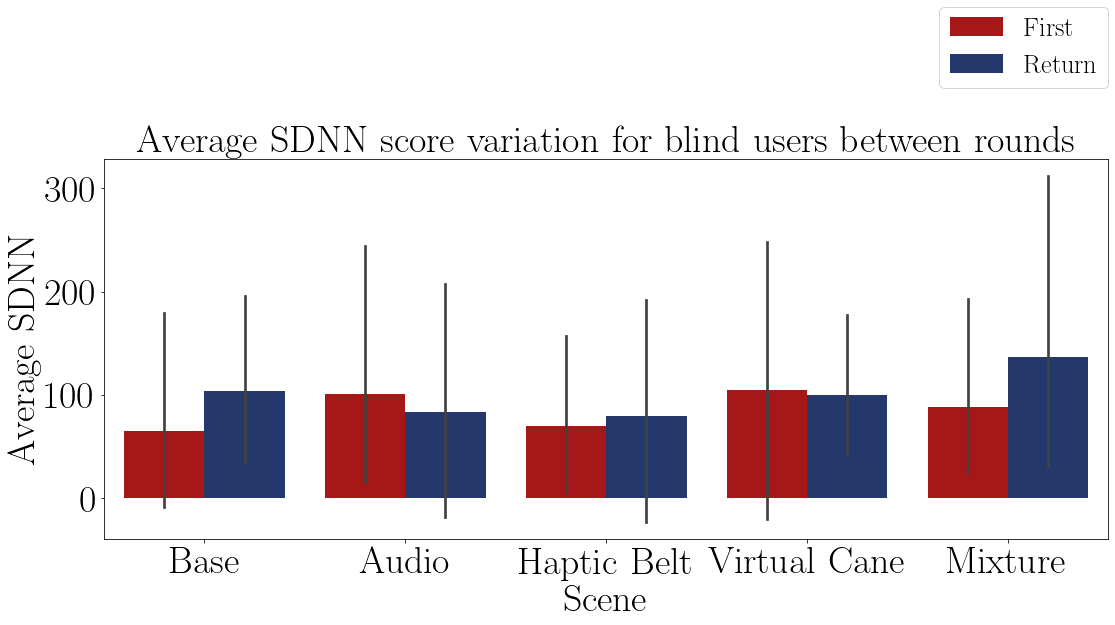
\includegraphics[width = 0.8\linewidth]{Resultados/ECG/Figuras/png/barplot_ecg_sdnn_scene_blind.png}
        %\resizebox{0.8\linewidth}{!}{
        %%% Creator: Matplotlib, PGF backend
%%
%% To include the figure in your LaTeX document, write
%%   \input{<filename>.pgf}
%%
%% Make sure the required packages are loaded in your preamble
%%   \usepackage{pgf}
%%
%% Figures using additional raster images can only be included by \input if
%% they are in the same directory as the main LaTeX file. For loading figures
%% from other directories you can use the `import` package
%%   \usepackage{import}
%%
%% and then include the figures with
%%   \import{<path to file>}{<filename>.pgf}
%%
%% Matplotlib used the following preamble
%%   \usepackage{fontspec}
%%
\begingroup%
\makeatletter%
\begin{pgfpicture}%
\pgfpathrectangle{\pgfpointorigin}{\pgfqpoint{15.369508in}{8.690562in}}%
\pgfusepath{use as bounding box, clip}%
\begin{pgfscope}%
\pgfsetbuttcap%
\pgfsetmiterjoin%
\pgfsetlinewidth{0.000000pt}%
\definecolor{currentstroke}{rgb}{1.000000,1.000000,1.000000}%
\pgfsetstrokecolor{currentstroke}%
\pgfsetstrokeopacity{0.000000}%
\pgfsetdash{}{0pt}%
\pgfpathmoveto{\pgfqpoint{0.000000in}{-0.000000in}}%
\pgfpathlineto{\pgfqpoint{15.369508in}{-0.000000in}}%
\pgfpathlineto{\pgfqpoint{15.369508in}{8.690562in}}%
\pgfpathlineto{\pgfqpoint{0.000000in}{8.690562in}}%
\pgfpathclose%
\pgfusepath{}%
\end{pgfscope}%
\begin{pgfscope}%
\pgfsetbuttcap%
\pgfsetmiterjoin%
\definecolor{currentfill}{rgb}{1.000000,1.000000,1.000000}%
\pgfsetfillcolor{currentfill}%
\pgfsetlinewidth{0.000000pt}%
\definecolor{currentstroke}{rgb}{0.000000,0.000000,0.000000}%
\pgfsetstrokecolor{currentstroke}%
\pgfsetstrokeopacity{0.000000}%
\pgfsetdash{}{0pt}%
\pgfpathmoveto{\pgfqpoint{1.319508in}{1.191562in}}%
\pgfpathlineto{\pgfqpoint{15.269508in}{1.191562in}}%
\pgfpathlineto{\pgfqpoint{15.269508in}{6.476562in}}%
\pgfpathlineto{\pgfqpoint{1.319508in}{6.476562in}}%
\pgfpathclose%
\pgfusepath{fill}%
\end{pgfscope}%
\begin{pgfscope}%
\pgfpathrectangle{\pgfqpoint{1.319508in}{1.191562in}}{\pgfqpoint{13.950000in}{5.285000in}}%
\pgfusepath{clip}%
\pgfsetbuttcap%
\pgfsetmiterjoin%
\definecolor{currentfill}{rgb}{0.651961,0.093137,0.093137}%
\pgfsetfillcolor{currentfill}%
\pgfsetlinewidth{0.000000pt}%
\definecolor{currentstroke}{rgb}{0.000000,0.000000,0.000000}%
\pgfsetstrokecolor{currentstroke}%
\pgfsetstrokeopacity{0.000000}%
\pgfsetdash{}{0pt}%
\pgfpathmoveto{\pgfqpoint{1.598508in}{5.432025in}}%
\pgfpathlineto{\pgfqpoint{2.714508in}{5.432025in}}%
\pgfpathlineto{\pgfqpoint{2.714508in}{4.583309in}}%
\pgfpathlineto{\pgfqpoint{1.598508in}{4.583309in}}%
\pgfpathclose%
\pgfusepath{fill}%
\end{pgfscope}%
\begin{pgfscope}%
\pgfpathrectangle{\pgfqpoint{1.319508in}{1.191562in}}{\pgfqpoint{13.950000in}{5.285000in}}%
\pgfusepath{clip}%
\pgfsetbuttcap%
\pgfsetmiterjoin%
\definecolor{currentfill}{rgb}{0.651961,0.093137,0.093137}%
\pgfsetfillcolor{currentfill}%
\pgfsetlinewidth{0.000000pt}%
\definecolor{currentstroke}{rgb}{0.000000,0.000000,0.000000}%
\pgfsetstrokecolor{currentstroke}%
\pgfsetstrokeopacity{0.000000}%
\pgfsetdash{}{0pt}%
\pgfpathmoveto{\pgfqpoint{4.388508in}{5.432025in}}%
\pgfpathlineto{\pgfqpoint{5.504508in}{5.432025in}}%
\pgfpathlineto{\pgfqpoint{5.504508in}{3.558465in}}%
\pgfpathlineto{\pgfqpoint{4.388508in}{3.558465in}}%
\pgfpathclose%
\pgfusepath{fill}%
\end{pgfscope}%
\begin{pgfscope}%
\pgfpathrectangle{\pgfqpoint{1.319508in}{1.191562in}}{\pgfqpoint{13.950000in}{5.285000in}}%
\pgfusepath{clip}%
\pgfsetbuttcap%
\pgfsetmiterjoin%
\definecolor{currentfill}{rgb}{0.651961,0.093137,0.093137}%
\pgfsetfillcolor{currentfill}%
\pgfsetlinewidth{0.000000pt}%
\definecolor{currentstroke}{rgb}{0.000000,0.000000,0.000000}%
\pgfsetstrokecolor{currentstroke}%
\pgfsetstrokeopacity{0.000000}%
\pgfsetdash{}{0pt}%
\pgfpathmoveto{\pgfqpoint{7.178508in}{5.432025in}}%
\pgfpathlineto{\pgfqpoint{8.294508in}{5.432025in}}%
\pgfpathlineto{\pgfqpoint{8.294508in}{4.476572in}}%
\pgfpathlineto{\pgfqpoint{7.178508in}{4.476572in}}%
\pgfpathclose%
\pgfusepath{fill}%
\end{pgfscope}%
\begin{pgfscope}%
\pgfpathrectangle{\pgfqpoint{1.319508in}{1.191562in}}{\pgfqpoint{13.950000in}{5.285000in}}%
\pgfusepath{clip}%
\pgfsetbuttcap%
\pgfsetmiterjoin%
\definecolor{currentfill}{rgb}{0.651961,0.093137,0.093137}%
\pgfsetfillcolor{currentfill}%
\pgfsetlinewidth{0.000000pt}%
\definecolor{currentstroke}{rgb}{0.000000,0.000000,0.000000}%
\pgfsetstrokecolor{currentstroke}%
\pgfsetstrokeopacity{0.000000}%
\pgfsetdash{}{0pt}%
\pgfpathmoveto{\pgfqpoint{9.968508in}{5.432025in}}%
\pgfpathlineto{\pgfqpoint{11.084508in}{5.432025in}}%
\pgfpathlineto{\pgfqpoint{11.084508in}{3.778608in}}%
\pgfpathlineto{\pgfqpoint{9.968508in}{3.778608in}}%
\pgfpathclose%
\pgfusepath{fill}%
\end{pgfscope}%
\begin{pgfscope}%
\pgfpathrectangle{\pgfqpoint{1.319508in}{1.191562in}}{\pgfqpoint{13.950000in}{5.285000in}}%
\pgfusepath{clip}%
\pgfsetbuttcap%
\pgfsetmiterjoin%
\definecolor{currentfill}{rgb}{0.651961,0.093137,0.093137}%
\pgfsetfillcolor{currentfill}%
\pgfsetlinewidth{0.000000pt}%
\definecolor{currentstroke}{rgb}{0.000000,0.000000,0.000000}%
\pgfsetstrokecolor{currentstroke}%
\pgfsetstrokeopacity{0.000000}%
\pgfsetdash{}{0pt}%
\pgfpathmoveto{\pgfqpoint{12.758508in}{5.432025in}}%
\pgfpathlineto{\pgfqpoint{13.874508in}{5.432025in}}%
\pgfpathlineto{\pgfqpoint{13.874508in}{4.339698in}}%
\pgfpathlineto{\pgfqpoint{12.758508in}{4.339698in}}%
\pgfpathclose%
\pgfusepath{fill}%
\end{pgfscope}%
\begin{pgfscope}%
\pgfpathrectangle{\pgfqpoint{1.319508in}{1.191562in}}{\pgfqpoint{13.950000in}{5.285000in}}%
\pgfusepath{clip}%
\pgfsetbuttcap%
\pgfsetmiterjoin%
\definecolor{currentfill}{rgb}{0.144608,0.218137,0.424020}%
\pgfsetfillcolor{currentfill}%
\pgfsetlinewidth{0.000000pt}%
\definecolor{currentstroke}{rgb}{0.000000,0.000000,0.000000}%
\pgfsetstrokecolor{currentstroke}%
\pgfsetstrokeopacity{0.000000}%
\pgfsetdash{}{0pt}%
\pgfpathmoveto{\pgfqpoint{2.714508in}{5.432025in}}%
\pgfpathlineto{\pgfqpoint{3.830508in}{5.432025in}}%
\pgfpathlineto{\pgfqpoint{3.830508in}{4.506389in}}%
\pgfpathlineto{\pgfqpoint{2.714508in}{4.506389in}}%
\pgfpathclose%
\pgfusepath{fill}%
\end{pgfscope}%
\begin{pgfscope}%
\pgfpathrectangle{\pgfqpoint{1.319508in}{1.191562in}}{\pgfqpoint{13.950000in}{5.285000in}}%
\pgfusepath{clip}%
\pgfsetbuttcap%
\pgfsetmiterjoin%
\definecolor{currentfill}{rgb}{0.144608,0.218137,0.424020}%
\pgfsetfillcolor{currentfill}%
\pgfsetlinewidth{0.000000pt}%
\definecolor{currentstroke}{rgb}{0.000000,0.000000,0.000000}%
\pgfsetstrokecolor{currentstroke}%
\pgfsetstrokeopacity{0.000000}%
\pgfsetdash{}{0pt}%
\pgfpathmoveto{\pgfqpoint{5.504508in}{5.432025in}}%
\pgfpathlineto{\pgfqpoint{6.620508in}{5.432025in}}%
\pgfpathlineto{\pgfqpoint{6.620508in}{3.808164in}}%
\pgfpathlineto{\pgfqpoint{5.504508in}{3.808164in}}%
\pgfpathclose%
\pgfusepath{fill}%
\end{pgfscope}%
\begin{pgfscope}%
\pgfpathrectangle{\pgfqpoint{1.319508in}{1.191562in}}{\pgfqpoint{13.950000in}{5.285000in}}%
\pgfusepath{clip}%
\pgfsetbuttcap%
\pgfsetmiterjoin%
\definecolor{currentfill}{rgb}{0.144608,0.218137,0.424020}%
\pgfsetfillcolor{currentfill}%
\pgfsetlinewidth{0.000000pt}%
\definecolor{currentstroke}{rgb}{0.000000,0.000000,0.000000}%
\pgfsetstrokecolor{currentstroke}%
\pgfsetstrokeopacity{0.000000}%
\pgfsetdash{}{0pt}%
\pgfpathmoveto{\pgfqpoint{8.294508in}{5.432025in}}%
\pgfpathlineto{\pgfqpoint{9.410508in}{5.432025in}}%
\pgfpathlineto{\pgfqpoint{9.410508in}{4.696413in}}%
\pgfpathlineto{\pgfqpoint{8.294508in}{4.696413in}}%
\pgfpathclose%
\pgfusepath{fill}%
\end{pgfscope}%
\begin{pgfscope}%
\pgfpathrectangle{\pgfqpoint{1.319508in}{1.191562in}}{\pgfqpoint{13.950000in}{5.285000in}}%
\pgfusepath{clip}%
\pgfsetbuttcap%
\pgfsetmiterjoin%
\definecolor{currentfill}{rgb}{0.144608,0.218137,0.424020}%
\pgfsetfillcolor{currentfill}%
\pgfsetlinewidth{0.000000pt}%
\definecolor{currentstroke}{rgb}{0.000000,0.000000,0.000000}%
\pgfsetstrokecolor{currentstroke}%
\pgfsetstrokeopacity{0.000000}%
\pgfsetdash{}{0pt}%
\pgfpathmoveto{\pgfqpoint{11.084508in}{5.432025in}}%
\pgfpathlineto{\pgfqpoint{12.200508in}{5.432025in}}%
\pgfpathlineto{\pgfqpoint{12.200508in}{4.423975in}}%
\pgfpathlineto{\pgfqpoint{11.084508in}{4.423975in}}%
\pgfpathclose%
\pgfusepath{fill}%
\end{pgfscope}%
\begin{pgfscope}%
\pgfpathrectangle{\pgfqpoint{1.319508in}{1.191562in}}{\pgfqpoint{13.950000in}{5.285000in}}%
\pgfusepath{clip}%
\pgfsetbuttcap%
\pgfsetmiterjoin%
\definecolor{currentfill}{rgb}{0.144608,0.218137,0.424020}%
\pgfsetfillcolor{currentfill}%
\pgfsetlinewidth{0.000000pt}%
\definecolor{currentstroke}{rgb}{0.000000,0.000000,0.000000}%
\pgfsetstrokecolor{currentstroke}%
\pgfsetstrokeopacity{0.000000}%
\pgfsetdash{}{0pt}%
\pgfpathmoveto{\pgfqpoint{13.874508in}{5.432025in}}%
\pgfpathlineto{\pgfqpoint{14.990508in}{5.432025in}}%
\pgfpathlineto{\pgfqpoint{14.990508in}{4.469000in}}%
\pgfpathlineto{\pgfqpoint{13.874508in}{4.469000in}}%
\pgfpathclose%
\pgfusepath{fill}%
\end{pgfscope}%
\begin{pgfscope}%
\pgfsetbuttcap%
\pgfsetroundjoin%
\definecolor{currentfill}{rgb}{0.000000,0.000000,0.000000}%
\pgfsetfillcolor{currentfill}%
\pgfsetlinewidth{0.803000pt}%
\definecolor{currentstroke}{rgb}{0.000000,0.000000,0.000000}%
\pgfsetstrokecolor{currentstroke}%
\pgfsetdash{}{0pt}%
\pgfsys@defobject{currentmarker}{\pgfqpoint{0.000000in}{-0.048611in}}{\pgfqpoint{0.000000in}{0.000000in}}{%
\pgfpathmoveto{\pgfqpoint{0.000000in}{0.000000in}}%
\pgfpathlineto{\pgfqpoint{0.000000in}{-0.048611in}}%
\pgfusepath{stroke,fill}%
}%
\begin{pgfscope}%
\pgfsys@transformshift{2.714508in}{1.191562in}%
\pgfsys@useobject{currentmarker}{}%
\end{pgfscope}%
\end{pgfscope}%
\begin{pgfscope}%
\definecolor{textcolor}{rgb}{0.000000,0.000000,0.000000}%
\pgfsetstrokecolor{textcolor}%
\pgfsetfillcolor{textcolor}%
\pgftext[x=2.714508in,y=1.094339in,,top]{\color{textcolor}\rmfamily\fontsize{38.016000}{45.619200}\selectfont Base}%
\end{pgfscope}%
\begin{pgfscope}%
\pgfsetbuttcap%
\pgfsetroundjoin%
\definecolor{currentfill}{rgb}{0.000000,0.000000,0.000000}%
\pgfsetfillcolor{currentfill}%
\pgfsetlinewidth{0.803000pt}%
\definecolor{currentstroke}{rgb}{0.000000,0.000000,0.000000}%
\pgfsetstrokecolor{currentstroke}%
\pgfsetdash{}{0pt}%
\pgfsys@defobject{currentmarker}{\pgfqpoint{0.000000in}{-0.048611in}}{\pgfqpoint{0.000000in}{0.000000in}}{%
\pgfpathmoveto{\pgfqpoint{0.000000in}{0.000000in}}%
\pgfpathlineto{\pgfqpoint{0.000000in}{-0.048611in}}%
\pgfusepath{stroke,fill}%
}%
\begin{pgfscope}%
\pgfsys@transformshift{5.504508in}{1.191562in}%
\pgfsys@useobject{currentmarker}{}%
\end{pgfscope}%
\end{pgfscope}%
\begin{pgfscope}%
\definecolor{textcolor}{rgb}{0.000000,0.000000,0.000000}%
\pgfsetstrokecolor{textcolor}%
\pgfsetfillcolor{textcolor}%
\pgftext[x=5.504508in,y=1.094339in,,top]{\color{textcolor}\rmfamily\fontsize{38.016000}{45.619200}\selectfont Audio}%
\end{pgfscope}%
\begin{pgfscope}%
\pgfsetbuttcap%
\pgfsetroundjoin%
\definecolor{currentfill}{rgb}{0.000000,0.000000,0.000000}%
\pgfsetfillcolor{currentfill}%
\pgfsetlinewidth{0.803000pt}%
\definecolor{currentstroke}{rgb}{0.000000,0.000000,0.000000}%
\pgfsetstrokecolor{currentstroke}%
\pgfsetdash{}{0pt}%
\pgfsys@defobject{currentmarker}{\pgfqpoint{0.000000in}{-0.048611in}}{\pgfqpoint{0.000000in}{0.000000in}}{%
\pgfpathmoveto{\pgfqpoint{0.000000in}{0.000000in}}%
\pgfpathlineto{\pgfqpoint{0.000000in}{-0.048611in}}%
\pgfusepath{stroke,fill}%
}%
\begin{pgfscope}%
\pgfsys@transformshift{8.294508in}{1.191562in}%
\pgfsys@useobject{currentmarker}{}%
\end{pgfscope}%
\end{pgfscope}%
\begin{pgfscope}%
\definecolor{textcolor}{rgb}{0.000000,0.000000,0.000000}%
\pgfsetstrokecolor{textcolor}%
\pgfsetfillcolor{textcolor}%
\pgftext[x=8.294508in,y=1.094339in,,top]{\color{textcolor}\rmfamily\fontsize{38.016000}{45.619200}\selectfont Haptic Belt}%
\end{pgfscope}%
\begin{pgfscope}%
\pgfsetbuttcap%
\pgfsetroundjoin%
\definecolor{currentfill}{rgb}{0.000000,0.000000,0.000000}%
\pgfsetfillcolor{currentfill}%
\pgfsetlinewidth{0.803000pt}%
\definecolor{currentstroke}{rgb}{0.000000,0.000000,0.000000}%
\pgfsetstrokecolor{currentstroke}%
\pgfsetdash{}{0pt}%
\pgfsys@defobject{currentmarker}{\pgfqpoint{0.000000in}{-0.048611in}}{\pgfqpoint{0.000000in}{0.000000in}}{%
\pgfpathmoveto{\pgfqpoint{0.000000in}{0.000000in}}%
\pgfpathlineto{\pgfqpoint{0.000000in}{-0.048611in}}%
\pgfusepath{stroke,fill}%
}%
\begin{pgfscope}%
\pgfsys@transformshift{11.084508in}{1.191562in}%
\pgfsys@useobject{currentmarker}{}%
\end{pgfscope}%
\end{pgfscope}%
\begin{pgfscope}%
\definecolor{textcolor}{rgb}{0.000000,0.000000,0.000000}%
\pgfsetstrokecolor{textcolor}%
\pgfsetfillcolor{textcolor}%
\pgftext[x=11.084508in,y=1.094339in,,top]{\color{textcolor}\rmfamily\fontsize{38.016000}{45.619200}\selectfont Virtual Cane}%
\end{pgfscope}%
\begin{pgfscope}%
\pgfsetbuttcap%
\pgfsetroundjoin%
\definecolor{currentfill}{rgb}{0.000000,0.000000,0.000000}%
\pgfsetfillcolor{currentfill}%
\pgfsetlinewidth{0.803000pt}%
\definecolor{currentstroke}{rgb}{0.000000,0.000000,0.000000}%
\pgfsetstrokecolor{currentstroke}%
\pgfsetdash{}{0pt}%
\pgfsys@defobject{currentmarker}{\pgfqpoint{0.000000in}{-0.048611in}}{\pgfqpoint{0.000000in}{0.000000in}}{%
\pgfpathmoveto{\pgfqpoint{0.000000in}{0.000000in}}%
\pgfpathlineto{\pgfqpoint{0.000000in}{-0.048611in}}%
\pgfusepath{stroke,fill}%
}%
\begin{pgfscope}%
\pgfsys@transformshift{13.874508in}{1.191562in}%
\pgfsys@useobject{currentmarker}{}%
\end{pgfscope}%
\end{pgfscope}%
\begin{pgfscope}%
\definecolor{textcolor}{rgb}{0.000000,0.000000,0.000000}%
\pgfsetstrokecolor{textcolor}%
\pgfsetfillcolor{textcolor}%
\pgftext[x=13.874508in,y=1.094339in,,top]{\color{textcolor}\rmfamily\fontsize{38.016000}{45.619200}\selectfont Mixture}%
\end{pgfscope}%
\begin{pgfscope}%
\definecolor{textcolor}{rgb}{0.000000,0.000000,0.000000}%
\pgfsetstrokecolor{textcolor}%
\pgfsetfillcolor{textcolor}%
\pgftext[x=8.294508in,y=0.569392in,,top]{\color{textcolor}\rmfamily\fontsize{38.016000}{45.619200}\selectfont Scene}%
\end{pgfscope}%
\begin{pgfscope}%
\pgfsetbuttcap%
\pgfsetroundjoin%
\definecolor{currentfill}{rgb}{0.000000,0.000000,0.000000}%
\pgfsetfillcolor{currentfill}%
\pgfsetlinewidth{0.803000pt}%
\definecolor{currentstroke}{rgb}{0.000000,0.000000,0.000000}%
\pgfsetstrokecolor{currentstroke}%
\pgfsetdash{}{0pt}%
\pgfsys@defobject{currentmarker}{\pgfqpoint{-0.048611in}{0.000000in}}{\pgfqpoint{-0.000000in}{0.000000in}}{%
\pgfpathmoveto{\pgfqpoint{-0.000000in}{0.000000in}}%
\pgfpathlineto{\pgfqpoint{-0.048611in}{0.000000in}}%
\pgfusepath{stroke,fill}%
}%
\begin{pgfscope}%
\pgfsys@transformshift{1.319508in}{1.767373in}%
\pgfsys@useobject{currentmarker}{}%
\end{pgfscope}%
\end{pgfscope}%
\begin{pgfscope}%
\definecolor{textcolor}{rgb}{0.000000,0.000000,0.000000}%
\pgfsetstrokecolor{textcolor}%
\pgfsetfillcolor{textcolor}%
\pgftext[x=0.636563in, y=1.584157in, left, base]{\color{textcolor}\rmfamily\fontsize{38.016000}{45.619200}\selectfont \(\displaystyle {\ensuremath{-}30}\)}%
\end{pgfscope}%
\begin{pgfscope}%
\pgfsetbuttcap%
\pgfsetroundjoin%
\definecolor{currentfill}{rgb}{0.000000,0.000000,0.000000}%
\pgfsetfillcolor{currentfill}%
\pgfsetlinewidth{0.803000pt}%
\definecolor{currentstroke}{rgb}{0.000000,0.000000,0.000000}%
\pgfsetstrokecolor{currentstroke}%
\pgfsetdash{}{0pt}%
\pgfsys@defobject{currentmarker}{\pgfqpoint{-0.048611in}{0.000000in}}{\pgfqpoint{-0.000000in}{0.000000in}}{%
\pgfpathmoveto{\pgfqpoint{-0.000000in}{0.000000in}}%
\pgfpathlineto{\pgfqpoint{-0.048611in}{0.000000in}}%
\pgfusepath{stroke,fill}%
}%
\begin{pgfscope}%
\pgfsys@transformshift{1.319508in}{2.988924in}%
\pgfsys@useobject{currentmarker}{}%
\end{pgfscope}%
\end{pgfscope}%
\begin{pgfscope}%
\definecolor{textcolor}{rgb}{0.000000,0.000000,0.000000}%
\pgfsetstrokecolor{textcolor}%
\pgfsetfillcolor{textcolor}%
\pgftext[x=0.636563in, y=2.805708in, left, base]{\color{textcolor}\rmfamily\fontsize{38.016000}{45.619200}\selectfont \(\displaystyle {\ensuremath{-}20}\)}%
\end{pgfscope}%
\begin{pgfscope}%
\pgfsetbuttcap%
\pgfsetroundjoin%
\definecolor{currentfill}{rgb}{0.000000,0.000000,0.000000}%
\pgfsetfillcolor{currentfill}%
\pgfsetlinewidth{0.803000pt}%
\definecolor{currentstroke}{rgb}{0.000000,0.000000,0.000000}%
\pgfsetstrokecolor{currentstroke}%
\pgfsetdash{}{0pt}%
\pgfsys@defobject{currentmarker}{\pgfqpoint{-0.048611in}{0.000000in}}{\pgfqpoint{-0.000000in}{0.000000in}}{%
\pgfpathmoveto{\pgfqpoint{-0.000000in}{0.000000in}}%
\pgfpathlineto{\pgfqpoint{-0.048611in}{0.000000in}}%
\pgfusepath{stroke,fill}%
}%
\begin{pgfscope}%
\pgfsys@transformshift{1.319508in}{4.210475in}%
\pgfsys@useobject{currentmarker}{}%
\end{pgfscope}%
\end{pgfscope}%
\begin{pgfscope}%
\definecolor{textcolor}{rgb}{0.000000,0.000000,0.000000}%
\pgfsetstrokecolor{textcolor}%
\pgfsetfillcolor{textcolor}%
\pgftext[x=0.636563in, y=4.027258in, left, base]{\color{textcolor}\rmfamily\fontsize{38.016000}{45.619200}\selectfont \(\displaystyle {\ensuremath{-}10}\)}%
\end{pgfscope}%
\begin{pgfscope}%
\pgfsetbuttcap%
\pgfsetroundjoin%
\definecolor{currentfill}{rgb}{0.000000,0.000000,0.000000}%
\pgfsetfillcolor{currentfill}%
\pgfsetlinewidth{0.803000pt}%
\definecolor{currentstroke}{rgb}{0.000000,0.000000,0.000000}%
\pgfsetstrokecolor{currentstroke}%
\pgfsetdash{}{0pt}%
\pgfsys@defobject{currentmarker}{\pgfqpoint{-0.048611in}{0.000000in}}{\pgfqpoint{-0.000000in}{0.000000in}}{%
\pgfpathmoveto{\pgfqpoint{-0.000000in}{0.000000in}}%
\pgfpathlineto{\pgfqpoint{-0.048611in}{0.000000in}}%
\pgfusepath{stroke,fill}%
}%
\begin{pgfscope}%
\pgfsys@transformshift{1.319508in}{5.432025in}%
\pgfsys@useobject{currentmarker}{}%
\end{pgfscope}%
\end{pgfscope}%
\begin{pgfscope}%
\definecolor{textcolor}{rgb}{0.000000,0.000000,0.000000}%
\pgfsetstrokecolor{textcolor}%
\pgfsetfillcolor{textcolor}%
\pgftext[x=1.063808in, y=5.248809in, left, base]{\color{textcolor}\rmfamily\fontsize{38.016000}{45.619200}\selectfont \(\displaystyle {0}\)}%
\end{pgfscope}%
\begin{pgfscope}%
\definecolor{textcolor}{rgb}{0.000000,0.000000,0.000000}%
\pgfsetstrokecolor{textcolor}%
\pgfsetfillcolor{textcolor}%
\pgftext[x=0.581008in,y=3.834062in,,bottom,rotate=90.000000]{\color{textcolor}\rmfamily\fontsize{38.016000}{45.619200}\selectfont Average BPM}%
\end{pgfscope}%
\begin{pgfscope}%
\pgfpathrectangle{\pgfqpoint{1.319508in}{1.191562in}}{\pgfqpoint{13.950000in}{5.285000in}}%
\pgfusepath{clip}%
\pgfsetrectcap%
\pgfsetroundjoin%
\pgfsetlinewidth{2.710125pt}%
\definecolor{currentstroke}{rgb}{0.260000,0.260000,0.260000}%
\pgfsetstrokecolor{currentstroke}%
\pgfsetdash{}{0pt}%
\pgfpathmoveto{\pgfqpoint{2.156508in}{2.751308in}}%
\pgfpathlineto{\pgfqpoint{2.156508in}{6.018483in}}%
\pgfusepath{stroke}%
\end{pgfscope}%
\begin{pgfscope}%
\pgfpathrectangle{\pgfqpoint{1.319508in}{1.191562in}}{\pgfqpoint{13.950000in}{5.285000in}}%
\pgfusepath{clip}%
\pgfsetrectcap%
\pgfsetroundjoin%
\pgfsetlinewidth{2.710125pt}%
\definecolor{currentstroke}{rgb}{0.260000,0.260000,0.260000}%
\pgfsetstrokecolor{currentstroke}%
\pgfsetdash{}{0pt}%
\pgfpathmoveto{\pgfqpoint{4.946508in}{1.431789in}}%
\pgfpathlineto{\pgfqpoint{4.946508in}{5.682086in}}%
\pgfusepath{stroke}%
\end{pgfscope}%
\begin{pgfscope}%
\pgfpathrectangle{\pgfqpoint{1.319508in}{1.191562in}}{\pgfqpoint{13.950000in}{5.285000in}}%
\pgfusepath{clip}%
\pgfsetrectcap%
\pgfsetroundjoin%
\pgfsetlinewidth{2.710125pt}%
\definecolor{currentstroke}{rgb}{0.260000,0.260000,0.260000}%
\pgfsetstrokecolor{currentstroke}%
\pgfsetdash{}{0pt}%
\pgfpathmoveto{\pgfqpoint{7.736508in}{2.678943in}}%
\pgfpathlineto{\pgfqpoint{7.736508in}{6.236334in}}%
\pgfusepath{stroke}%
\end{pgfscope}%
\begin{pgfscope}%
\pgfpathrectangle{\pgfqpoint{1.319508in}{1.191562in}}{\pgfqpoint{13.950000in}{5.285000in}}%
\pgfusepath{clip}%
\pgfsetrectcap%
\pgfsetroundjoin%
\pgfsetlinewidth{2.710125pt}%
\definecolor{currentstroke}{rgb}{0.260000,0.260000,0.260000}%
\pgfsetstrokecolor{currentstroke}%
\pgfsetdash{}{0pt}%
\pgfpathmoveto{\pgfqpoint{10.526508in}{2.047721in}}%
\pgfpathlineto{\pgfqpoint{10.526508in}{5.510294in}}%
\pgfusepath{stroke}%
\end{pgfscope}%
\begin{pgfscope}%
\pgfpathrectangle{\pgfqpoint{1.319508in}{1.191562in}}{\pgfqpoint{13.950000in}{5.285000in}}%
\pgfusepath{clip}%
\pgfsetrectcap%
\pgfsetroundjoin%
\pgfsetlinewidth{2.710125pt}%
\definecolor{currentstroke}{rgb}{0.260000,0.260000,0.260000}%
\pgfsetstrokecolor{currentstroke}%
\pgfsetdash{}{0pt}%
\pgfpathmoveto{\pgfqpoint{13.316508in}{3.163834in}}%
\pgfpathlineto{\pgfqpoint{13.316508in}{5.543100in}}%
\pgfusepath{stroke}%
\end{pgfscope}%
\begin{pgfscope}%
\pgfpathrectangle{\pgfqpoint{1.319508in}{1.191562in}}{\pgfqpoint{13.950000in}{5.285000in}}%
\pgfusepath{clip}%
\pgfsetrectcap%
\pgfsetroundjoin%
\pgfsetlinewidth{2.710125pt}%
\definecolor{currentstroke}{rgb}{0.260000,0.260000,0.260000}%
\pgfsetstrokecolor{currentstroke}%
\pgfsetdash{}{0pt}%
\pgfpathmoveto{\pgfqpoint{3.272508in}{3.222854in}}%
\pgfpathlineto{\pgfqpoint{3.272508in}{5.709606in}}%
\pgfusepath{stroke}%
\end{pgfscope}%
\begin{pgfscope}%
\pgfpathrectangle{\pgfqpoint{1.319508in}{1.191562in}}{\pgfqpoint{13.950000in}{5.285000in}}%
\pgfusepath{clip}%
\pgfsetrectcap%
\pgfsetroundjoin%
\pgfsetlinewidth{2.710125pt}%
\definecolor{currentstroke}{rgb}{0.260000,0.260000,0.260000}%
\pgfsetstrokecolor{currentstroke}%
\pgfsetdash{}{0pt}%
\pgfpathmoveto{\pgfqpoint{6.062508in}{1.933256in}}%
\pgfpathlineto{\pgfqpoint{6.062508in}{5.541904in}}%
\pgfusepath{stroke}%
\end{pgfscope}%
\begin{pgfscope}%
\pgfpathrectangle{\pgfqpoint{1.319508in}{1.191562in}}{\pgfqpoint{13.950000in}{5.285000in}}%
\pgfusepath{clip}%
\pgfsetrectcap%
\pgfsetroundjoin%
\pgfsetlinewidth{2.710125pt}%
\definecolor{currentstroke}{rgb}{0.260000,0.260000,0.260000}%
\pgfsetstrokecolor{currentstroke}%
\pgfsetdash{}{0pt}%
\pgfpathmoveto{\pgfqpoint{8.852508in}{3.694214in}}%
\pgfpathlineto{\pgfqpoint{8.852508in}{5.935485in}}%
\pgfusepath{stroke}%
\end{pgfscope}%
\begin{pgfscope}%
\pgfpathrectangle{\pgfqpoint{1.319508in}{1.191562in}}{\pgfqpoint{13.950000in}{5.285000in}}%
\pgfusepath{clip}%
\pgfsetrectcap%
\pgfsetroundjoin%
\pgfsetlinewidth{2.710125pt}%
\definecolor{currentstroke}{rgb}{0.260000,0.260000,0.260000}%
\pgfsetstrokecolor{currentstroke}%
\pgfsetdash{}{0pt}%
\pgfpathmoveto{\pgfqpoint{11.642508in}{3.336183in}}%
\pgfpathlineto{\pgfqpoint{11.642508in}{5.657013in}}%
\pgfusepath{stroke}%
\end{pgfscope}%
\begin{pgfscope}%
\pgfpathrectangle{\pgfqpoint{1.319508in}{1.191562in}}{\pgfqpoint{13.950000in}{5.285000in}}%
\pgfusepath{clip}%
\pgfsetrectcap%
\pgfsetroundjoin%
\pgfsetlinewidth{2.710125pt}%
\definecolor{currentstroke}{rgb}{0.260000,0.260000,0.260000}%
\pgfsetstrokecolor{currentstroke}%
\pgfsetdash{}{0pt}%
\pgfpathmoveto{\pgfqpoint{14.432508in}{3.718499in}}%
\pgfpathlineto{\pgfqpoint{14.432508in}{5.571045in}}%
\pgfusepath{stroke}%
\end{pgfscope}%
\begin{pgfscope}%
\pgfsetrectcap%
\pgfsetmiterjoin%
\pgfsetlinewidth{0.803000pt}%
\definecolor{currentstroke}{rgb}{0.000000,0.000000,0.000000}%
\pgfsetstrokecolor{currentstroke}%
\pgfsetdash{}{0pt}%
\pgfpathmoveto{\pgfqpoint{1.319508in}{1.191562in}}%
\pgfpathlineto{\pgfqpoint{1.319508in}{6.476562in}}%
\pgfusepath{stroke}%
\end{pgfscope}%
\begin{pgfscope}%
\pgfsetrectcap%
\pgfsetmiterjoin%
\pgfsetlinewidth{0.803000pt}%
\definecolor{currentstroke}{rgb}{0.000000,0.000000,0.000000}%
\pgfsetstrokecolor{currentstroke}%
\pgfsetdash{}{0pt}%
\pgfpathmoveto{\pgfqpoint{15.269508in}{1.191562in}}%
\pgfpathlineto{\pgfqpoint{15.269508in}{6.476562in}}%
\pgfusepath{stroke}%
\end{pgfscope}%
\begin{pgfscope}%
\pgfsetrectcap%
\pgfsetmiterjoin%
\pgfsetlinewidth{0.803000pt}%
\definecolor{currentstroke}{rgb}{0.000000,0.000000,0.000000}%
\pgfsetstrokecolor{currentstroke}%
\pgfsetdash{}{0pt}%
\pgfpathmoveto{\pgfqpoint{1.319508in}{1.191562in}}%
\pgfpathlineto{\pgfqpoint{15.269508in}{1.191562in}}%
\pgfusepath{stroke}%
\end{pgfscope}%
\begin{pgfscope}%
\pgfsetrectcap%
\pgfsetmiterjoin%
\pgfsetlinewidth{0.803000pt}%
\definecolor{currentstroke}{rgb}{0.000000,0.000000,0.000000}%
\pgfsetstrokecolor{currentstroke}%
\pgfsetdash{}{0pt}%
\pgfpathmoveto{\pgfqpoint{1.319508in}{6.476562in}}%
\pgfpathlineto{\pgfqpoint{15.269508in}{6.476562in}}%
\pgfusepath{stroke}%
\end{pgfscope}%
\begin{pgfscope}%
\definecolor{textcolor}{rgb}{0.000000,0.000000,0.000000}%
\pgfsetstrokecolor{textcolor}%
\pgfsetfillcolor{textcolor}%
\pgftext[x=8.294508in,y=6.584273in,,base]{\color{textcolor}\rmfamily\fontsize{38.016000}{45.619200}\selectfont Average BPM score variation for blind users between rounds}%
\end{pgfscope}%
\begin{pgfscope}%
\pgfsetbuttcap%
\pgfsetmiterjoin%
\definecolor{currentfill}{rgb}{1.000000,1.000000,1.000000}%
\pgfsetfillcolor{currentfill}%
\pgfsetfillopacity{0.800000}%
\pgfsetlinewidth{1.003750pt}%
\definecolor{currentstroke}{rgb}{0.800000,0.800000,0.800000}%
\pgfsetstrokecolor{currentstroke}%
\pgfsetstrokeopacity{0.800000}%
\pgfsetdash{}{0pt}%
\pgfpathmoveto{\pgfqpoint{12.990308in}{7.457562in}}%
\pgfpathlineto{\pgfqpoint{15.196175in}{7.457562in}}%
\pgfpathquadraticcurveto{\pgfqpoint{15.269508in}{7.457562in}}{\pgfqpoint{15.269508in}{7.530896in}}%
\pgfpathlineto{\pgfqpoint{15.269508in}{8.517228in}}%
\pgfpathquadraticcurveto{\pgfqpoint{15.269508in}{8.590562in}}{\pgfqpoint{15.196175in}{8.590562in}}%
\pgfpathlineto{\pgfqpoint{12.990308in}{8.590562in}}%
\pgfpathquadraticcurveto{\pgfqpoint{12.916975in}{8.590562in}}{\pgfqpoint{12.916975in}{8.517228in}}%
\pgfpathlineto{\pgfqpoint{12.916975in}{7.530896in}}%
\pgfpathquadraticcurveto{\pgfqpoint{12.916975in}{7.457562in}}{\pgfqpoint{12.990308in}{7.457562in}}%
\pgfpathclose%
\pgfusepath{stroke,fill}%
\end{pgfscope}%
\begin{pgfscope}%
\pgfsetbuttcap%
\pgfsetmiterjoin%
\definecolor{currentfill}{rgb}{0.651961,0.093137,0.093137}%
\pgfsetfillcolor{currentfill}%
\pgfsetlinewidth{0.000000pt}%
\definecolor{currentstroke}{rgb}{0.000000,0.000000,0.000000}%
\pgfsetstrokecolor{currentstroke}%
\pgfsetstrokeopacity{0.000000}%
\pgfsetdash{}{0pt}%
\pgfpathmoveto{\pgfqpoint{13.063642in}{8.187228in}}%
\pgfpathlineto{\pgfqpoint{13.796975in}{8.187228in}}%
\pgfpathlineto{\pgfqpoint{13.796975in}{8.443895in}}%
\pgfpathlineto{\pgfqpoint{13.063642in}{8.443895in}}%
\pgfpathclose%
\pgfusepath{fill}%
\end{pgfscope}%
\begin{pgfscope}%
\definecolor{textcolor}{rgb}{0.000000,0.000000,0.000000}%
\pgfsetstrokecolor{textcolor}%
\pgfsetfillcolor{textcolor}%
\pgftext[x=14.090308in,y=8.187228in,left,base]{\color{textcolor}\rmfamily\fontsize{26.400000}{31.680000}\selectfont First}%
\end{pgfscope}%
\begin{pgfscope}%
\pgfsetbuttcap%
\pgfsetmiterjoin%
\definecolor{currentfill}{rgb}{0.144608,0.218137,0.424020}%
\pgfsetfillcolor{currentfill}%
\pgfsetlinewidth{0.000000pt}%
\definecolor{currentstroke}{rgb}{0.000000,0.000000,0.000000}%
\pgfsetstrokecolor{currentstroke}%
\pgfsetstrokeopacity{0.000000}%
\pgfsetdash{}{0pt}%
\pgfpathmoveto{\pgfqpoint{13.063642in}{7.675729in}}%
\pgfpathlineto{\pgfqpoint{13.796975in}{7.675729in}}%
\pgfpathlineto{\pgfqpoint{13.796975in}{7.932395in}}%
\pgfpathlineto{\pgfqpoint{13.063642in}{7.932395in}}%
\pgfpathclose%
\pgfusepath{fill}%
\end{pgfscope}%
\begin{pgfscope}%
\definecolor{textcolor}{rgb}{0.000000,0.000000,0.000000}%
\pgfsetstrokecolor{textcolor}%
\pgfsetfillcolor{textcolor}%
\pgftext[x=14.090308in,y=7.675729in,left,base]{\color{textcolor}\rmfamily\fontsize{26.400000}{31.680000}\selectfont Return}%
\end{pgfscope}%
\end{pgfpicture}%
\makeatother%
\endgroup%

        %}
        \caption{Bar plot of the standard deviation of the heart of the blind participants on each method.}
        \label{fig:barplot_ecg_sdnn_scene_blind}
    \end{minipage}
    \begin{minipage}{\textwidth}
        \centering
        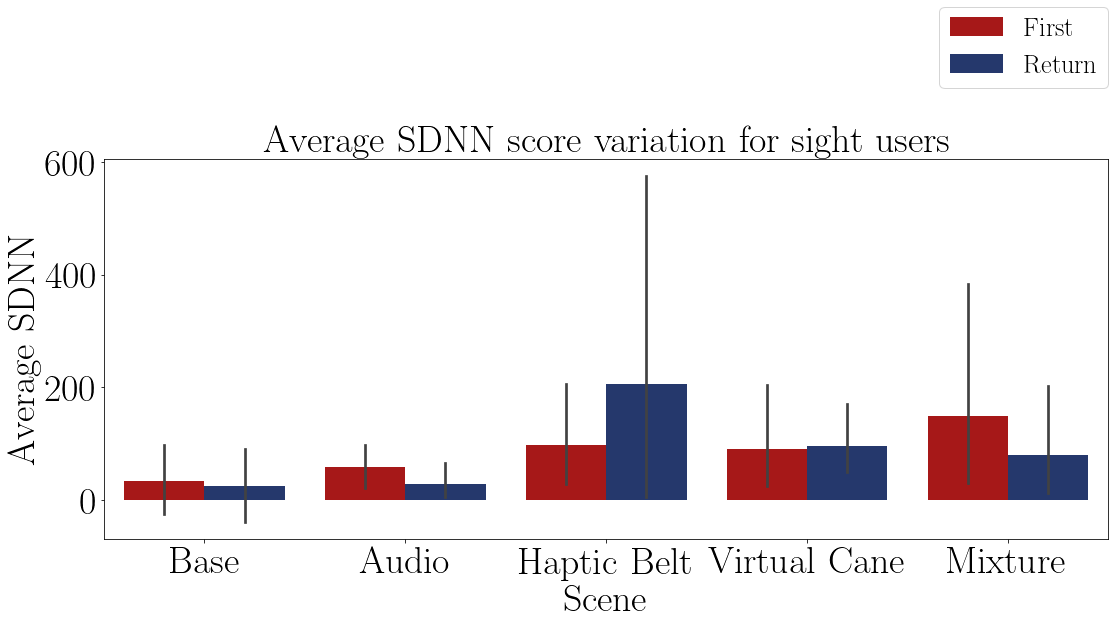
\includegraphics[width = 0.8\linewidth]{Resultados/ECG/Figuras/png/barplot_ecg_sdnn_scene_sight.png}
        %\resizebox{0.6\linewidth}{!}{
        %%% Creator: Matplotlib, PGF backend
%%
%% To include the figure in your LaTeX document, write
%%   \input{<filename>.pgf}
%%
%% Make sure the required packages are loaded in your preamble
%%   \usepackage{pgf}
%%
%% Figures using additional raster images can only be included by \input if
%% they are in the same directory as the main LaTeX file. For loading figures
%% from other directories you can use the `import` package
%%   \usepackage{import}
%%
%% and then include the figures with
%%   \import{<path to file>}{<filename>.pgf}
%%
%% Matplotlib used the following preamble
%%   \usepackage{fontspec}
%%
\begingroup%
\makeatletter%
\begin{pgfpicture}%
\pgfpathrectangle{\pgfpointorigin}{\pgfqpoint{15.369508in}{8.690562in}}%
\pgfusepath{use as bounding box, clip}%
\begin{pgfscope}%
\pgfsetbuttcap%
\pgfsetmiterjoin%
\pgfsetlinewidth{0.000000pt}%
\definecolor{currentstroke}{rgb}{1.000000,1.000000,1.000000}%
\pgfsetstrokecolor{currentstroke}%
\pgfsetstrokeopacity{0.000000}%
\pgfsetdash{}{0pt}%
\pgfpathmoveto{\pgfqpoint{0.000000in}{-0.000000in}}%
\pgfpathlineto{\pgfqpoint{15.369508in}{-0.000000in}}%
\pgfpathlineto{\pgfqpoint{15.369508in}{8.690562in}}%
\pgfpathlineto{\pgfqpoint{0.000000in}{8.690562in}}%
\pgfpathclose%
\pgfusepath{}%
\end{pgfscope}%
\begin{pgfscope}%
\pgfsetbuttcap%
\pgfsetmiterjoin%
\definecolor{currentfill}{rgb}{1.000000,1.000000,1.000000}%
\pgfsetfillcolor{currentfill}%
\pgfsetlinewidth{0.000000pt}%
\definecolor{currentstroke}{rgb}{0.000000,0.000000,0.000000}%
\pgfsetstrokecolor{currentstroke}%
\pgfsetstrokeopacity{0.000000}%
\pgfsetdash{}{0pt}%
\pgfpathmoveto{\pgfqpoint{1.319508in}{1.191562in}}%
\pgfpathlineto{\pgfqpoint{15.269508in}{1.191562in}}%
\pgfpathlineto{\pgfqpoint{15.269508in}{6.476562in}}%
\pgfpathlineto{\pgfqpoint{1.319508in}{6.476562in}}%
\pgfpathclose%
\pgfusepath{fill}%
\end{pgfscope}%
\begin{pgfscope}%
\pgfpathrectangle{\pgfqpoint{1.319508in}{1.191562in}}{\pgfqpoint{13.950000in}{5.285000in}}%
\pgfusepath{clip}%
\pgfsetbuttcap%
\pgfsetmiterjoin%
\definecolor{currentfill}{rgb}{0.651961,0.093137,0.093137}%
\pgfsetfillcolor{currentfill}%
\pgfsetlinewidth{0.000000pt}%
\definecolor{currentstroke}{rgb}{0.000000,0.000000,0.000000}%
\pgfsetstrokecolor{currentstroke}%
\pgfsetstrokeopacity{0.000000}%
\pgfsetdash{}{0pt}%
\pgfpathmoveto{\pgfqpoint{1.598508in}{4.680673in}}%
\pgfpathlineto{\pgfqpoint{2.714508in}{4.680673in}}%
\pgfpathlineto{\pgfqpoint{2.714508in}{4.741049in}}%
\pgfpathlineto{\pgfqpoint{1.598508in}{4.741049in}}%
\pgfpathclose%
\pgfusepath{fill}%
\end{pgfscope}%
\begin{pgfscope}%
\pgfpathrectangle{\pgfqpoint{1.319508in}{1.191562in}}{\pgfqpoint{13.950000in}{5.285000in}}%
\pgfusepath{clip}%
\pgfsetbuttcap%
\pgfsetmiterjoin%
\definecolor{currentfill}{rgb}{0.651961,0.093137,0.093137}%
\pgfsetfillcolor{currentfill}%
\pgfsetlinewidth{0.000000pt}%
\definecolor{currentstroke}{rgb}{0.000000,0.000000,0.000000}%
\pgfsetstrokecolor{currentstroke}%
\pgfsetstrokeopacity{0.000000}%
\pgfsetdash{}{0pt}%
\pgfpathmoveto{\pgfqpoint{4.388508in}{4.680673in}}%
\pgfpathlineto{\pgfqpoint{5.504508in}{4.680673in}}%
\pgfpathlineto{\pgfqpoint{5.504508in}{3.662866in}}%
\pgfpathlineto{\pgfqpoint{4.388508in}{3.662866in}}%
\pgfpathclose%
\pgfusepath{fill}%
\end{pgfscope}%
\begin{pgfscope}%
\pgfpathrectangle{\pgfqpoint{1.319508in}{1.191562in}}{\pgfqpoint{13.950000in}{5.285000in}}%
\pgfusepath{clip}%
\pgfsetbuttcap%
\pgfsetmiterjoin%
\definecolor{currentfill}{rgb}{0.651961,0.093137,0.093137}%
\pgfsetfillcolor{currentfill}%
\pgfsetlinewidth{0.000000pt}%
\definecolor{currentstroke}{rgb}{0.000000,0.000000,0.000000}%
\pgfsetstrokecolor{currentstroke}%
\pgfsetstrokeopacity{0.000000}%
\pgfsetdash{}{0pt}%
\pgfpathmoveto{\pgfqpoint{7.178508in}{4.680673in}}%
\pgfpathlineto{\pgfqpoint{8.294508in}{4.680673in}}%
\pgfpathlineto{\pgfqpoint{8.294508in}{3.215289in}}%
\pgfpathlineto{\pgfqpoint{7.178508in}{3.215289in}}%
\pgfpathclose%
\pgfusepath{fill}%
\end{pgfscope}%
\begin{pgfscope}%
\pgfpathrectangle{\pgfqpoint{1.319508in}{1.191562in}}{\pgfqpoint{13.950000in}{5.285000in}}%
\pgfusepath{clip}%
\pgfsetbuttcap%
\pgfsetmiterjoin%
\definecolor{currentfill}{rgb}{0.651961,0.093137,0.093137}%
\pgfsetfillcolor{currentfill}%
\pgfsetlinewidth{0.000000pt}%
\definecolor{currentstroke}{rgb}{0.000000,0.000000,0.000000}%
\pgfsetstrokecolor{currentstroke}%
\pgfsetstrokeopacity{0.000000}%
\pgfsetdash{}{0pt}%
\pgfpathmoveto{\pgfqpoint{9.968508in}{4.680673in}}%
\pgfpathlineto{\pgfqpoint{11.084508in}{4.680673in}}%
\pgfpathlineto{\pgfqpoint{11.084508in}{3.425459in}}%
\pgfpathlineto{\pgfqpoint{9.968508in}{3.425459in}}%
\pgfpathclose%
\pgfusepath{fill}%
\end{pgfscope}%
\begin{pgfscope}%
\pgfpathrectangle{\pgfqpoint{1.319508in}{1.191562in}}{\pgfqpoint{13.950000in}{5.285000in}}%
\pgfusepath{clip}%
\pgfsetbuttcap%
\pgfsetmiterjoin%
\definecolor{currentfill}{rgb}{0.651961,0.093137,0.093137}%
\pgfsetfillcolor{currentfill}%
\pgfsetlinewidth{0.000000pt}%
\definecolor{currentstroke}{rgb}{0.000000,0.000000,0.000000}%
\pgfsetstrokecolor{currentstroke}%
\pgfsetstrokeopacity{0.000000}%
\pgfsetdash{}{0pt}%
\pgfpathmoveto{\pgfqpoint{12.758508in}{4.680673in}}%
\pgfpathlineto{\pgfqpoint{13.874508in}{4.680673in}}%
\pgfpathlineto{\pgfqpoint{13.874508in}{3.378145in}}%
\pgfpathlineto{\pgfqpoint{12.758508in}{3.378145in}}%
\pgfpathclose%
\pgfusepath{fill}%
\end{pgfscope}%
\begin{pgfscope}%
\pgfpathrectangle{\pgfqpoint{1.319508in}{1.191562in}}{\pgfqpoint{13.950000in}{5.285000in}}%
\pgfusepath{clip}%
\pgfsetbuttcap%
\pgfsetmiterjoin%
\definecolor{currentfill}{rgb}{0.144608,0.218137,0.424020}%
\pgfsetfillcolor{currentfill}%
\pgfsetlinewidth{0.000000pt}%
\definecolor{currentstroke}{rgb}{0.000000,0.000000,0.000000}%
\pgfsetstrokecolor{currentstroke}%
\pgfsetstrokeopacity{0.000000}%
\pgfsetdash{}{0pt}%
\pgfpathmoveto{\pgfqpoint{2.714508in}{4.680673in}}%
\pgfpathlineto{\pgfqpoint{3.830508in}{4.680673in}}%
\pgfpathlineto{\pgfqpoint{3.830508in}{4.383066in}}%
\pgfpathlineto{\pgfqpoint{2.714508in}{4.383066in}}%
\pgfpathclose%
\pgfusepath{fill}%
\end{pgfscope}%
\begin{pgfscope}%
\pgfpathrectangle{\pgfqpoint{1.319508in}{1.191562in}}{\pgfqpoint{13.950000in}{5.285000in}}%
\pgfusepath{clip}%
\pgfsetbuttcap%
\pgfsetmiterjoin%
\definecolor{currentfill}{rgb}{0.144608,0.218137,0.424020}%
\pgfsetfillcolor{currentfill}%
\pgfsetlinewidth{0.000000pt}%
\definecolor{currentstroke}{rgb}{0.000000,0.000000,0.000000}%
\pgfsetstrokecolor{currentstroke}%
\pgfsetstrokeopacity{0.000000}%
\pgfsetdash{}{0pt}%
\pgfpathmoveto{\pgfqpoint{5.504508in}{4.680673in}}%
\pgfpathlineto{\pgfqpoint{6.620508in}{4.680673in}}%
\pgfpathlineto{\pgfqpoint{6.620508in}{4.244260in}}%
\pgfpathlineto{\pgfqpoint{5.504508in}{4.244260in}}%
\pgfpathclose%
\pgfusepath{fill}%
\end{pgfscope}%
\begin{pgfscope}%
\pgfpathrectangle{\pgfqpoint{1.319508in}{1.191562in}}{\pgfqpoint{13.950000in}{5.285000in}}%
\pgfusepath{clip}%
\pgfsetbuttcap%
\pgfsetmiterjoin%
\definecolor{currentfill}{rgb}{0.144608,0.218137,0.424020}%
\pgfsetfillcolor{currentfill}%
\pgfsetlinewidth{0.000000pt}%
\definecolor{currentstroke}{rgb}{0.000000,0.000000,0.000000}%
\pgfsetstrokecolor{currentstroke}%
\pgfsetstrokeopacity{0.000000}%
\pgfsetdash{}{0pt}%
\pgfpathmoveto{\pgfqpoint{8.294508in}{4.680673in}}%
\pgfpathlineto{\pgfqpoint{9.410508in}{4.680673in}}%
\pgfpathlineto{\pgfqpoint{9.410508in}{3.234717in}}%
\pgfpathlineto{\pgfqpoint{8.294508in}{3.234717in}}%
\pgfpathclose%
\pgfusepath{fill}%
\end{pgfscope}%
\begin{pgfscope}%
\pgfpathrectangle{\pgfqpoint{1.319508in}{1.191562in}}{\pgfqpoint{13.950000in}{5.285000in}}%
\pgfusepath{clip}%
\pgfsetbuttcap%
\pgfsetmiterjoin%
\definecolor{currentfill}{rgb}{0.144608,0.218137,0.424020}%
\pgfsetfillcolor{currentfill}%
\pgfsetlinewidth{0.000000pt}%
\definecolor{currentstroke}{rgb}{0.000000,0.000000,0.000000}%
\pgfsetstrokecolor{currentstroke}%
\pgfsetstrokeopacity{0.000000}%
\pgfsetdash{}{0pt}%
\pgfpathmoveto{\pgfqpoint{11.084508in}{4.680673in}}%
\pgfpathlineto{\pgfqpoint{12.200508in}{4.680673in}}%
\pgfpathlineto{\pgfqpoint{12.200508in}{3.302703in}}%
\pgfpathlineto{\pgfqpoint{11.084508in}{3.302703in}}%
\pgfpathclose%
\pgfusepath{fill}%
\end{pgfscope}%
\begin{pgfscope}%
\pgfpathrectangle{\pgfqpoint{1.319508in}{1.191562in}}{\pgfqpoint{13.950000in}{5.285000in}}%
\pgfusepath{clip}%
\pgfsetbuttcap%
\pgfsetmiterjoin%
\definecolor{currentfill}{rgb}{0.144608,0.218137,0.424020}%
\pgfsetfillcolor{currentfill}%
\pgfsetlinewidth{0.000000pt}%
\definecolor{currentstroke}{rgb}{0.000000,0.000000,0.000000}%
\pgfsetstrokecolor{currentstroke}%
\pgfsetstrokeopacity{0.000000}%
\pgfsetdash{}{0pt}%
\pgfpathmoveto{\pgfqpoint{13.874508in}{4.680673in}}%
\pgfpathlineto{\pgfqpoint{14.990508in}{4.680673in}}%
\pgfpathlineto{\pgfqpoint{14.990508in}{3.868838in}}%
\pgfpathlineto{\pgfqpoint{13.874508in}{3.868838in}}%
\pgfpathclose%
\pgfusepath{fill}%
\end{pgfscope}%
\begin{pgfscope}%
\pgfsetbuttcap%
\pgfsetroundjoin%
\definecolor{currentfill}{rgb}{0.000000,0.000000,0.000000}%
\pgfsetfillcolor{currentfill}%
\pgfsetlinewidth{0.803000pt}%
\definecolor{currentstroke}{rgb}{0.000000,0.000000,0.000000}%
\pgfsetstrokecolor{currentstroke}%
\pgfsetdash{}{0pt}%
\pgfsys@defobject{currentmarker}{\pgfqpoint{0.000000in}{-0.048611in}}{\pgfqpoint{0.000000in}{0.000000in}}{%
\pgfpathmoveto{\pgfqpoint{0.000000in}{0.000000in}}%
\pgfpathlineto{\pgfqpoint{0.000000in}{-0.048611in}}%
\pgfusepath{stroke,fill}%
}%
\begin{pgfscope}%
\pgfsys@transformshift{2.714508in}{1.191562in}%
\pgfsys@useobject{currentmarker}{}%
\end{pgfscope}%
\end{pgfscope}%
\begin{pgfscope}%
\definecolor{textcolor}{rgb}{0.000000,0.000000,0.000000}%
\pgfsetstrokecolor{textcolor}%
\pgfsetfillcolor{textcolor}%
\pgftext[x=2.714508in,y=1.094339in,,top]{\color{textcolor}\rmfamily\fontsize{38.016000}{45.619200}\selectfont Base}%
\end{pgfscope}%
\begin{pgfscope}%
\pgfsetbuttcap%
\pgfsetroundjoin%
\definecolor{currentfill}{rgb}{0.000000,0.000000,0.000000}%
\pgfsetfillcolor{currentfill}%
\pgfsetlinewidth{0.803000pt}%
\definecolor{currentstroke}{rgb}{0.000000,0.000000,0.000000}%
\pgfsetstrokecolor{currentstroke}%
\pgfsetdash{}{0pt}%
\pgfsys@defobject{currentmarker}{\pgfqpoint{0.000000in}{-0.048611in}}{\pgfqpoint{0.000000in}{0.000000in}}{%
\pgfpathmoveto{\pgfqpoint{0.000000in}{0.000000in}}%
\pgfpathlineto{\pgfqpoint{0.000000in}{-0.048611in}}%
\pgfusepath{stroke,fill}%
}%
\begin{pgfscope}%
\pgfsys@transformshift{5.504508in}{1.191562in}%
\pgfsys@useobject{currentmarker}{}%
\end{pgfscope}%
\end{pgfscope}%
\begin{pgfscope}%
\definecolor{textcolor}{rgb}{0.000000,0.000000,0.000000}%
\pgfsetstrokecolor{textcolor}%
\pgfsetfillcolor{textcolor}%
\pgftext[x=5.504508in,y=1.094339in,,top]{\color{textcolor}\rmfamily\fontsize{38.016000}{45.619200}\selectfont Audio}%
\end{pgfscope}%
\begin{pgfscope}%
\pgfsetbuttcap%
\pgfsetroundjoin%
\definecolor{currentfill}{rgb}{0.000000,0.000000,0.000000}%
\pgfsetfillcolor{currentfill}%
\pgfsetlinewidth{0.803000pt}%
\definecolor{currentstroke}{rgb}{0.000000,0.000000,0.000000}%
\pgfsetstrokecolor{currentstroke}%
\pgfsetdash{}{0pt}%
\pgfsys@defobject{currentmarker}{\pgfqpoint{0.000000in}{-0.048611in}}{\pgfqpoint{0.000000in}{0.000000in}}{%
\pgfpathmoveto{\pgfqpoint{0.000000in}{0.000000in}}%
\pgfpathlineto{\pgfqpoint{0.000000in}{-0.048611in}}%
\pgfusepath{stroke,fill}%
}%
\begin{pgfscope}%
\pgfsys@transformshift{8.294508in}{1.191562in}%
\pgfsys@useobject{currentmarker}{}%
\end{pgfscope}%
\end{pgfscope}%
\begin{pgfscope}%
\definecolor{textcolor}{rgb}{0.000000,0.000000,0.000000}%
\pgfsetstrokecolor{textcolor}%
\pgfsetfillcolor{textcolor}%
\pgftext[x=8.294508in,y=1.094339in,,top]{\color{textcolor}\rmfamily\fontsize{38.016000}{45.619200}\selectfont Haptic Belt}%
\end{pgfscope}%
\begin{pgfscope}%
\pgfsetbuttcap%
\pgfsetroundjoin%
\definecolor{currentfill}{rgb}{0.000000,0.000000,0.000000}%
\pgfsetfillcolor{currentfill}%
\pgfsetlinewidth{0.803000pt}%
\definecolor{currentstroke}{rgb}{0.000000,0.000000,0.000000}%
\pgfsetstrokecolor{currentstroke}%
\pgfsetdash{}{0pt}%
\pgfsys@defobject{currentmarker}{\pgfqpoint{0.000000in}{-0.048611in}}{\pgfqpoint{0.000000in}{0.000000in}}{%
\pgfpathmoveto{\pgfqpoint{0.000000in}{0.000000in}}%
\pgfpathlineto{\pgfqpoint{0.000000in}{-0.048611in}}%
\pgfusepath{stroke,fill}%
}%
\begin{pgfscope}%
\pgfsys@transformshift{11.084508in}{1.191562in}%
\pgfsys@useobject{currentmarker}{}%
\end{pgfscope}%
\end{pgfscope}%
\begin{pgfscope}%
\definecolor{textcolor}{rgb}{0.000000,0.000000,0.000000}%
\pgfsetstrokecolor{textcolor}%
\pgfsetfillcolor{textcolor}%
\pgftext[x=11.084508in,y=1.094339in,,top]{\color{textcolor}\rmfamily\fontsize{38.016000}{45.619200}\selectfont Virtual Cane}%
\end{pgfscope}%
\begin{pgfscope}%
\pgfsetbuttcap%
\pgfsetroundjoin%
\definecolor{currentfill}{rgb}{0.000000,0.000000,0.000000}%
\pgfsetfillcolor{currentfill}%
\pgfsetlinewidth{0.803000pt}%
\definecolor{currentstroke}{rgb}{0.000000,0.000000,0.000000}%
\pgfsetstrokecolor{currentstroke}%
\pgfsetdash{}{0pt}%
\pgfsys@defobject{currentmarker}{\pgfqpoint{0.000000in}{-0.048611in}}{\pgfqpoint{0.000000in}{0.000000in}}{%
\pgfpathmoveto{\pgfqpoint{0.000000in}{0.000000in}}%
\pgfpathlineto{\pgfqpoint{0.000000in}{-0.048611in}}%
\pgfusepath{stroke,fill}%
}%
\begin{pgfscope}%
\pgfsys@transformshift{13.874508in}{1.191562in}%
\pgfsys@useobject{currentmarker}{}%
\end{pgfscope}%
\end{pgfscope}%
\begin{pgfscope}%
\definecolor{textcolor}{rgb}{0.000000,0.000000,0.000000}%
\pgfsetstrokecolor{textcolor}%
\pgfsetfillcolor{textcolor}%
\pgftext[x=13.874508in,y=1.094339in,,top]{\color{textcolor}\rmfamily\fontsize{38.016000}{45.619200}\selectfont Mixture}%
\end{pgfscope}%
\begin{pgfscope}%
\definecolor{textcolor}{rgb}{0.000000,0.000000,0.000000}%
\pgfsetstrokecolor{textcolor}%
\pgfsetfillcolor{textcolor}%
\pgftext[x=8.294508in,y=0.569392in,,top]{\color{textcolor}\rmfamily\fontsize{38.016000}{45.619200}\selectfont Scene}%
\end{pgfscope}%
\begin{pgfscope}%
\pgfsetbuttcap%
\pgfsetroundjoin%
\definecolor{currentfill}{rgb}{0.000000,0.000000,0.000000}%
\pgfsetfillcolor{currentfill}%
\pgfsetlinewidth{0.803000pt}%
\definecolor{currentstroke}{rgb}{0.000000,0.000000,0.000000}%
\pgfsetstrokecolor{currentstroke}%
\pgfsetdash{}{0pt}%
\pgfsys@defobject{currentmarker}{\pgfqpoint{-0.048611in}{0.000000in}}{\pgfqpoint{-0.000000in}{0.000000in}}{%
\pgfpathmoveto{\pgfqpoint{-0.000000in}{0.000000in}}%
\pgfpathlineto{\pgfqpoint{-0.048611in}{0.000000in}}%
\pgfusepath{stroke,fill}%
}%
\begin{pgfscope}%
\pgfsys@transformshift{1.319508in}{1.759960in}%
\pgfsys@useobject{currentmarker}{}%
\end{pgfscope}%
\end{pgfscope}%
\begin{pgfscope}%
\definecolor{textcolor}{rgb}{0.000000,0.000000,0.000000}%
\pgfsetstrokecolor{textcolor}%
\pgfsetfillcolor{textcolor}%
\pgftext[x=0.636563in, y=1.576744in, left, base]{\color{textcolor}\rmfamily\fontsize{38.016000}{45.619200}\selectfont \(\displaystyle {\ensuremath{-}20}\)}%
\end{pgfscope}%
\begin{pgfscope}%
\pgfsetbuttcap%
\pgfsetroundjoin%
\definecolor{currentfill}{rgb}{0.000000,0.000000,0.000000}%
\pgfsetfillcolor{currentfill}%
\pgfsetlinewidth{0.803000pt}%
\definecolor{currentstroke}{rgb}{0.000000,0.000000,0.000000}%
\pgfsetstrokecolor{currentstroke}%
\pgfsetdash{}{0pt}%
\pgfsys@defobject{currentmarker}{\pgfqpoint{-0.048611in}{0.000000in}}{\pgfqpoint{-0.000000in}{0.000000in}}{%
\pgfpathmoveto{\pgfqpoint{-0.000000in}{0.000000in}}%
\pgfpathlineto{\pgfqpoint{-0.048611in}{0.000000in}}%
\pgfusepath{stroke,fill}%
}%
\begin{pgfscope}%
\pgfsys@transformshift{1.319508in}{3.220316in}%
\pgfsys@useobject{currentmarker}{}%
\end{pgfscope}%
\end{pgfscope}%
\begin{pgfscope}%
\definecolor{textcolor}{rgb}{0.000000,0.000000,0.000000}%
\pgfsetstrokecolor{textcolor}%
\pgfsetfillcolor{textcolor}%
\pgftext[x=0.636563in, y=3.037100in, left, base]{\color{textcolor}\rmfamily\fontsize{38.016000}{45.619200}\selectfont \(\displaystyle {\ensuremath{-}10}\)}%
\end{pgfscope}%
\begin{pgfscope}%
\pgfsetbuttcap%
\pgfsetroundjoin%
\definecolor{currentfill}{rgb}{0.000000,0.000000,0.000000}%
\pgfsetfillcolor{currentfill}%
\pgfsetlinewidth{0.803000pt}%
\definecolor{currentstroke}{rgb}{0.000000,0.000000,0.000000}%
\pgfsetstrokecolor{currentstroke}%
\pgfsetdash{}{0pt}%
\pgfsys@defobject{currentmarker}{\pgfqpoint{-0.048611in}{0.000000in}}{\pgfqpoint{-0.000000in}{0.000000in}}{%
\pgfpathmoveto{\pgfqpoint{-0.000000in}{0.000000in}}%
\pgfpathlineto{\pgfqpoint{-0.048611in}{0.000000in}}%
\pgfusepath{stroke,fill}%
}%
\begin{pgfscope}%
\pgfsys@transformshift{1.319508in}{4.680673in}%
\pgfsys@useobject{currentmarker}{}%
\end{pgfscope}%
\end{pgfscope}%
\begin{pgfscope}%
\definecolor{textcolor}{rgb}{0.000000,0.000000,0.000000}%
\pgfsetstrokecolor{textcolor}%
\pgfsetfillcolor{textcolor}%
\pgftext[x=1.063808in, y=4.497457in, left, base]{\color{textcolor}\rmfamily\fontsize{38.016000}{45.619200}\selectfont \(\displaystyle {0}\)}%
\end{pgfscope}%
\begin{pgfscope}%
\pgfsetbuttcap%
\pgfsetroundjoin%
\definecolor{currentfill}{rgb}{0.000000,0.000000,0.000000}%
\pgfsetfillcolor{currentfill}%
\pgfsetlinewidth{0.803000pt}%
\definecolor{currentstroke}{rgb}{0.000000,0.000000,0.000000}%
\pgfsetstrokecolor{currentstroke}%
\pgfsetdash{}{0pt}%
\pgfsys@defobject{currentmarker}{\pgfqpoint{-0.048611in}{0.000000in}}{\pgfqpoint{-0.000000in}{0.000000in}}{%
\pgfpathmoveto{\pgfqpoint{-0.000000in}{0.000000in}}%
\pgfpathlineto{\pgfqpoint{-0.048611in}{0.000000in}}%
\pgfusepath{stroke,fill}%
}%
\begin{pgfscope}%
\pgfsys@transformshift{1.319508in}{6.141029in}%
\pgfsys@useobject{currentmarker}{}%
\end{pgfscope}%
\end{pgfscope}%
\begin{pgfscope}%
\definecolor{textcolor}{rgb}{0.000000,0.000000,0.000000}%
\pgfsetstrokecolor{textcolor}%
\pgfsetfillcolor{textcolor}%
\pgftext[x=0.905330in, y=5.957813in, left, base]{\color{textcolor}\rmfamily\fontsize{38.016000}{45.619200}\selectfont \(\displaystyle {10}\)}%
\end{pgfscope}%
\begin{pgfscope}%
\definecolor{textcolor}{rgb}{0.000000,0.000000,0.000000}%
\pgfsetstrokecolor{textcolor}%
\pgfsetfillcolor{textcolor}%
\pgftext[x=0.581008in,y=3.834062in,,bottom,rotate=90.000000]{\color{textcolor}\rmfamily\fontsize{38.016000}{45.619200}\selectfont Average BPM}%
\end{pgfscope}%
\begin{pgfscope}%
\pgfpathrectangle{\pgfqpoint{1.319508in}{1.191562in}}{\pgfqpoint{13.950000in}{5.285000in}}%
\pgfusepath{clip}%
\pgfsetrectcap%
\pgfsetroundjoin%
\pgfsetlinewidth{2.710125pt}%
\definecolor{currentstroke}{rgb}{0.260000,0.260000,0.260000}%
\pgfsetstrokecolor{currentstroke}%
\pgfsetdash{}{0pt}%
\pgfpathmoveto{\pgfqpoint{2.156508in}{3.970565in}}%
\pgfpathlineto{\pgfqpoint{2.156508in}{5.766272in}}%
\pgfusepath{stroke}%
\end{pgfscope}%
\begin{pgfscope}%
\pgfpathrectangle{\pgfqpoint{1.319508in}{1.191562in}}{\pgfqpoint{13.950000in}{5.285000in}}%
\pgfusepath{clip}%
\pgfsetrectcap%
\pgfsetroundjoin%
\pgfsetlinewidth{2.710125pt}%
\definecolor{currentstroke}{rgb}{0.260000,0.260000,0.260000}%
\pgfsetstrokecolor{currentstroke}%
\pgfsetdash{}{0pt}%
\pgfpathmoveto{\pgfqpoint{4.946508in}{2.464955in}}%
\pgfpathlineto{\pgfqpoint{4.946508in}{4.860777in}}%
\pgfusepath{stroke}%
\end{pgfscope}%
\begin{pgfscope}%
\pgfpathrectangle{\pgfqpoint{1.319508in}{1.191562in}}{\pgfqpoint{13.950000in}{5.285000in}}%
\pgfusepath{clip}%
\pgfsetrectcap%
\pgfsetroundjoin%
\pgfsetlinewidth{2.710125pt}%
\definecolor{currentstroke}{rgb}{0.260000,0.260000,0.260000}%
\pgfsetstrokecolor{currentstroke}%
\pgfsetdash{}{0pt}%
\pgfpathmoveto{\pgfqpoint{7.736508in}{1.998402in}}%
\pgfpathlineto{\pgfqpoint{7.736508in}{3.936033in}}%
\pgfusepath{stroke}%
\end{pgfscope}%
\begin{pgfscope}%
\pgfpathrectangle{\pgfqpoint{1.319508in}{1.191562in}}{\pgfqpoint{13.950000in}{5.285000in}}%
\pgfusepath{clip}%
\pgfsetrectcap%
\pgfsetroundjoin%
\pgfsetlinewidth{2.710125pt}%
\definecolor{currentstroke}{rgb}{0.260000,0.260000,0.260000}%
\pgfsetstrokecolor{currentstroke}%
\pgfsetdash{}{0pt}%
\pgfpathmoveto{\pgfqpoint{10.526508in}{2.220154in}}%
\pgfpathlineto{\pgfqpoint{10.526508in}{4.478297in}}%
\pgfusepath{stroke}%
\end{pgfscope}%
\begin{pgfscope}%
\pgfpathrectangle{\pgfqpoint{1.319508in}{1.191562in}}{\pgfqpoint{13.950000in}{5.285000in}}%
\pgfusepath{clip}%
\pgfsetrectcap%
\pgfsetroundjoin%
\pgfsetlinewidth{2.710125pt}%
\definecolor{currentstroke}{rgb}{0.260000,0.260000,0.260000}%
\pgfsetstrokecolor{currentstroke}%
\pgfsetdash{}{0pt}%
\pgfpathmoveto{\pgfqpoint{13.316508in}{1.431789in}}%
\pgfpathlineto{\pgfqpoint{13.316508in}{4.887907in}}%
\pgfusepath{stroke}%
\end{pgfscope}%
\begin{pgfscope}%
\pgfpathrectangle{\pgfqpoint{1.319508in}{1.191562in}}{\pgfqpoint{13.950000in}{5.285000in}}%
\pgfusepath{clip}%
\pgfsetrectcap%
\pgfsetroundjoin%
\pgfsetlinewidth{2.710125pt}%
\definecolor{currentstroke}{rgb}{0.260000,0.260000,0.260000}%
\pgfsetstrokecolor{currentstroke}%
\pgfsetdash{}{0pt}%
\pgfpathmoveto{\pgfqpoint{3.272508in}{3.162266in}}%
\pgfpathlineto{\pgfqpoint{3.272508in}{6.236334in}}%
\pgfusepath{stroke}%
\end{pgfscope}%
\begin{pgfscope}%
\pgfpathrectangle{\pgfqpoint{1.319508in}{1.191562in}}{\pgfqpoint{13.950000in}{5.285000in}}%
\pgfusepath{clip}%
\pgfsetrectcap%
\pgfsetroundjoin%
\pgfsetlinewidth{2.710125pt}%
\definecolor{currentstroke}{rgb}{0.260000,0.260000,0.260000}%
\pgfsetstrokecolor{currentstroke}%
\pgfsetdash{}{0pt}%
\pgfpathmoveto{\pgfqpoint{6.062508in}{3.502466in}}%
\pgfpathlineto{\pgfqpoint{6.062508in}{5.158738in}}%
\pgfusepath{stroke}%
\end{pgfscope}%
\begin{pgfscope}%
\pgfpathrectangle{\pgfqpoint{1.319508in}{1.191562in}}{\pgfqpoint{13.950000in}{5.285000in}}%
\pgfusepath{clip}%
\pgfsetrectcap%
\pgfsetroundjoin%
\pgfsetlinewidth{2.710125pt}%
\definecolor{currentstroke}{rgb}{0.260000,0.260000,0.260000}%
\pgfsetstrokecolor{currentstroke}%
\pgfsetdash{}{0pt}%
\pgfpathmoveto{\pgfqpoint{8.852508in}{1.700683in}}%
\pgfpathlineto{\pgfqpoint{8.852508in}{4.445199in}}%
\pgfusepath{stroke}%
\end{pgfscope}%
\begin{pgfscope}%
\pgfpathrectangle{\pgfqpoint{1.319508in}{1.191562in}}{\pgfqpoint{13.950000in}{5.285000in}}%
\pgfusepath{clip}%
\pgfsetrectcap%
\pgfsetroundjoin%
\pgfsetlinewidth{2.710125pt}%
\definecolor{currentstroke}{rgb}{0.260000,0.260000,0.260000}%
\pgfsetstrokecolor{currentstroke}%
\pgfsetdash{}{0pt}%
\pgfpathmoveto{\pgfqpoint{11.642508in}{2.443751in}}%
\pgfpathlineto{\pgfqpoint{11.642508in}{4.161655in}}%
\pgfusepath{stroke}%
\end{pgfscope}%
\begin{pgfscope}%
\pgfpathrectangle{\pgfqpoint{1.319508in}{1.191562in}}{\pgfqpoint{13.950000in}{5.285000in}}%
\pgfusepath{clip}%
\pgfsetrectcap%
\pgfsetroundjoin%
\pgfsetlinewidth{2.710125pt}%
\definecolor{currentstroke}{rgb}{0.260000,0.260000,0.260000}%
\pgfsetstrokecolor{currentstroke}%
\pgfsetdash{}{0pt}%
\pgfpathmoveto{\pgfqpoint{14.432508in}{2.359990in}}%
\pgfpathlineto{\pgfqpoint{14.432508in}{5.480374in}}%
\pgfusepath{stroke}%
\end{pgfscope}%
\begin{pgfscope}%
\pgfsetrectcap%
\pgfsetmiterjoin%
\pgfsetlinewidth{0.803000pt}%
\definecolor{currentstroke}{rgb}{0.000000,0.000000,0.000000}%
\pgfsetstrokecolor{currentstroke}%
\pgfsetdash{}{0pt}%
\pgfpathmoveto{\pgfqpoint{1.319508in}{1.191562in}}%
\pgfpathlineto{\pgfqpoint{1.319508in}{6.476562in}}%
\pgfusepath{stroke}%
\end{pgfscope}%
\begin{pgfscope}%
\pgfsetrectcap%
\pgfsetmiterjoin%
\pgfsetlinewidth{0.803000pt}%
\definecolor{currentstroke}{rgb}{0.000000,0.000000,0.000000}%
\pgfsetstrokecolor{currentstroke}%
\pgfsetdash{}{0pt}%
\pgfpathmoveto{\pgfqpoint{15.269508in}{1.191562in}}%
\pgfpathlineto{\pgfqpoint{15.269508in}{6.476562in}}%
\pgfusepath{stroke}%
\end{pgfscope}%
\begin{pgfscope}%
\pgfsetrectcap%
\pgfsetmiterjoin%
\pgfsetlinewidth{0.803000pt}%
\definecolor{currentstroke}{rgb}{0.000000,0.000000,0.000000}%
\pgfsetstrokecolor{currentstroke}%
\pgfsetdash{}{0pt}%
\pgfpathmoveto{\pgfqpoint{1.319508in}{1.191562in}}%
\pgfpathlineto{\pgfqpoint{15.269508in}{1.191562in}}%
\pgfusepath{stroke}%
\end{pgfscope}%
\begin{pgfscope}%
\pgfsetrectcap%
\pgfsetmiterjoin%
\pgfsetlinewidth{0.803000pt}%
\definecolor{currentstroke}{rgb}{0.000000,0.000000,0.000000}%
\pgfsetstrokecolor{currentstroke}%
\pgfsetdash{}{0pt}%
\pgfpathmoveto{\pgfqpoint{1.319508in}{6.476562in}}%
\pgfpathlineto{\pgfqpoint{15.269508in}{6.476562in}}%
\pgfusepath{stroke}%
\end{pgfscope}%
\begin{pgfscope}%
\definecolor{textcolor}{rgb}{0.000000,0.000000,0.000000}%
\pgfsetstrokecolor{textcolor}%
\pgfsetfillcolor{textcolor}%
\pgftext[x=8.294508in,y=6.584273in,,base]{\color{textcolor}\rmfamily\fontsize{38.016000}{45.619200}\selectfont Average BPM score variation for sight users}%
\end{pgfscope}%
\begin{pgfscope}%
\pgfsetbuttcap%
\pgfsetmiterjoin%
\definecolor{currentfill}{rgb}{1.000000,1.000000,1.000000}%
\pgfsetfillcolor{currentfill}%
\pgfsetfillopacity{0.800000}%
\pgfsetlinewidth{1.003750pt}%
\definecolor{currentstroke}{rgb}{0.800000,0.800000,0.800000}%
\pgfsetstrokecolor{currentstroke}%
\pgfsetstrokeopacity{0.800000}%
\pgfsetdash{}{0pt}%
\pgfpathmoveto{\pgfqpoint{12.990308in}{7.457562in}}%
\pgfpathlineto{\pgfqpoint{15.196175in}{7.457562in}}%
\pgfpathquadraticcurveto{\pgfqpoint{15.269508in}{7.457562in}}{\pgfqpoint{15.269508in}{7.530896in}}%
\pgfpathlineto{\pgfqpoint{15.269508in}{8.517228in}}%
\pgfpathquadraticcurveto{\pgfqpoint{15.269508in}{8.590562in}}{\pgfqpoint{15.196175in}{8.590562in}}%
\pgfpathlineto{\pgfqpoint{12.990308in}{8.590562in}}%
\pgfpathquadraticcurveto{\pgfqpoint{12.916975in}{8.590562in}}{\pgfqpoint{12.916975in}{8.517228in}}%
\pgfpathlineto{\pgfqpoint{12.916975in}{7.530896in}}%
\pgfpathquadraticcurveto{\pgfqpoint{12.916975in}{7.457562in}}{\pgfqpoint{12.990308in}{7.457562in}}%
\pgfpathclose%
\pgfusepath{stroke,fill}%
\end{pgfscope}%
\begin{pgfscope}%
\pgfsetbuttcap%
\pgfsetmiterjoin%
\definecolor{currentfill}{rgb}{0.651961,0.093137,0.093137}%
\pgfsetfillcolor{currentfill}%
\pgfsetlinewidth{0.000000pt}%
\definecolor{currentstroke}{rgb}{0.000000,0.000000,0.000000}%
\pgfsetstrokecolor{currentstroke}%
\pgfsetstrokeopacity{0.000000}%
\pgfsetdash{}{0pt}%
\pgfpathmoveto{\pgfqpoint{13.063642in}{8.187228in}}%
\pgfpathlineto{\pgfqpoint{13.796975in}{8.187228in}}%
\pgfpathlineto{\pgfqpoint{13.796975in}{8.443895in}}%
\pgfpathlineto{\pgfqpoint{13.063642in}{8.443895in}}%
\pgfpathclose%
\pgfusepath{fill}%
\end{pgfscope}%
\begin{pgfscope}%
\definecolor{textcolor}{rgb}{0.000000,0.000000,0.000000}%
\pgfsetstrokecolor{textcolor}%
\pgfsetfillcolor{textcolor}%
\pgftext[x=14.090308in,y=8.187228in,left,base]{\color{textcolor}\rmfamily\fontsize{26.400000}{31.680000}\selectfont First}%
\end{pgfscope}%
\begin{pgfscope}%
\pgfsetbuttcap%
\pgfsetmiterjoin%
\definecolor{currentfill}{rgb}{0.144608,0.218137,0.424020}%
\pgfsetfillcolor{currentfill}%
\pgfsetlinewidth{0.000000pt}%
\definecolor{currentstroke}{rgb}{0.000000,0.000000,0.000000}%
\pgfsetstrokecolor{currentstroke}%
\pgfsetstrokeopacity{0.000000}%
\pgfsetdash{}{0pt}%
\pgfpathmoveto{\pgfqpoint{13.063642in}{7.675729in}}%
\pgfpathlineto{\pgfqpoint{13.796975in}{7.675729in}}%
\pgfpathlineto{\pgfqpoint{13.796975in}{7.932395in}}%
\pgfpathlineto{\pgfqpoint{13.063642in}{7.932395in}}%
\pgfpathclose%
\pgfusepath{fill}%
\end{pgfscope}%
\begin{pgfscope}%
\definecolor{textcolor}{rgb}{0.000000,0.000000,0.000000}%
\pgfsetstrokecolor{textcolor}%
\pgfsetfillcolor{textcolor}%
\pgftext[x=14.090308in,y=7.675729in,left,base]{\color{textcolor}\rmfamily\fontsize{26.400000}{31.680000}\selectfont Return}%
\end{pgfscope}%
\end{pgfpicture}%
\makeatother%
\endgroup%
    
        %}
        \caption{Bar plot of the standard deviation of the heart of the sighted participants on each method.}
        \label{fig:barplot_ecg_sdnn_scene_sight}
    \end{minipage}
\end{figure}

The Figures \ref{fig:boxplot_ecg_sdnn_box_scene} and \ref{fig:barplot_ecg_sdnn_global} show a comparison between both groups. They show that both groups had a similar standard deviation of the heartbeat and that means a similar mental workload in both groups.

\begin{figure}[!htb]
    %\centering
    \begin{minipage}{.45\linewidth}
        \centering
        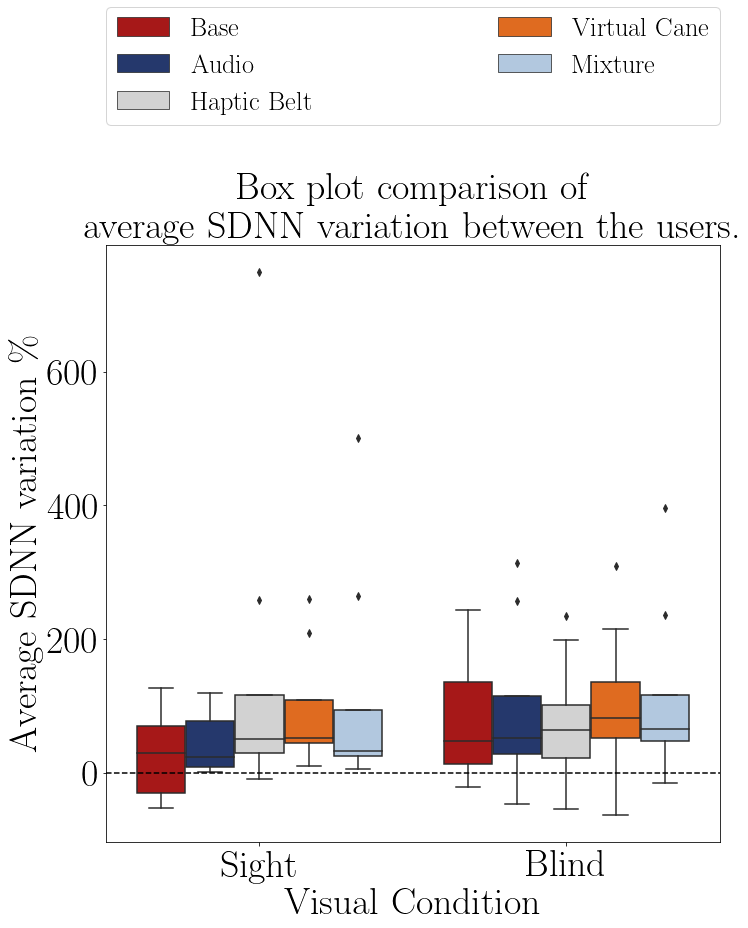
\includegraphics[width = \linewidth]{Resultados/ECG/Figuras/png/boxplot_ecg_sdnn_box_scene.png}
        %%% Creator: Matplotlib, PGF backend
%%
%% To include the figure in your LaTeX document, write
%%   \input{<filename>.pgf}
%%
%% Make sure the required packages are loaded in your preamble
%%   \usepackage{pgf}
%%
%% and, on pdftex
%%   \usepackage[utf8]{inputenc}\DeclareUnicodeCharacter{2212}{-}
%%
%% or, on luatex and xetex
%%   \usepackage{unicode-math}
%%
%% Figures using additional raster images can only be included by \input if
%% they are in the same directory as the main LaTeX file. For loading figures
%% from other directories you can use the `import` package
%%   \usepackage{import}
%%
%% and then include the figures with
%%   \import{<path to file>}{<filename>.pgf}
%%
%% Matplotlib used the following preamble
%%   \usepackage{url}
%%   \usepackage{unicode-math}
%%   \setmainfont{DejaVu Serif}
%%   \usepackage{fontspec}
%%
\begingroup%
\makeatletter%
\begin{pgfpicture}%
\pgfpathrectangle{\pgfpointorigin}{\pgfqpoint{12.196638in}{14.528848in}}%
\pgfusepath{use as bounding box, clip}%
\begin{pgfscope}%
\pgfsetbuttcap%
\pgfsetmiterjoin%
\pgfsetlinewidth{0.000000pt}%
\definecolor{currentstroke}{rgb}{1.000000,1.000000,1.000000}%
\pgfsetstrokecolor{currentstroke}%
\pgfsetstrokeopacity{0.000000}%
\pgfsetdash{}{0pt}%
\pgfpathmoveto{\pgfqpoint{0.000000in}{0.000000in}}%
\pgfpathlineto{\pgfqpoint{12.196638in}{0.000000in}}%
\pgfpathlineto{\pgfqpoint{12.196638in}{14.528848in}}%
\pgfpathlineto{\pgfqpoint{0.000000in}{14.528848in}}%
\pgfpathclose%
\pgfusepath{}%
\end{pgfscope}%
\begin{pgfscope}%
\pgfsetbuttcap%
\pgfsetmiterjoin%
\definecolor{currentfill}{rgb}{1.000000,1.000000,1.000000}%
\pgfsetfillcolor{currentfill}%
\pgfsetlinewidth{0.000000pt}%
\definecolor{currentstroke}{rgb}{0.000000,0.000000,0.000000}%
\pgfsetstrokecolor{currentstroke}%
\pgfsetstrokeopacity{0.000000}%
\pgfsetdash{}{0pt}%
\pgfpathmoveto{\pgfqpoint{1.246638in}{1.110648in}}%
\pgfpathlineto{\pgfqpoint{12.096638in}{1.110648in}}%
\pgfpathlineto{\pgfqpoint{12.096638in}{11.680648in}}%
\pgfpathlineto{\pgfqpoint{1.246638in}{11.680648in}}%
\pgfpathclose%
\pgfusepath{fill}%
\end{pgfscope}%
\begin{pgfscope}%
\pgfpathrectangle{\pgfqpoint{1.246638in}{1.110648in}}{\pgfqpoint{10.850000in}{10.570000in}}%
\pgfusepath{clip}%
\pgfsetbuttcap%
\pgfsetmiterjoin%
\definecolor{currentfill}{rgb}{0.651961,0.093137,0.093137}%
\pgfsetfillcolor{currentfill}%
\pgfsetlinewidth{1.505625pt}%
\definecolor{currentstroke}{rgb}{0.168627,0.168627,0.168627}%
\pgfsetstrokecolor{currentstroke}%
\pgfsetdash{}{0pt}%
\pgfpathmoveto{\pgfqpoint{1.797818in}{11.200194in}}%
\pgfpathlineto{\pgfqpoint{2.648458in}{11.200194in}}%
\pgfpathlineto{\pgfqpoint{2.648458in}{11.200194in}}%
\pgfpathlineto{\pgfqpoint{1.797818in}{11.200194in}}%
\pgfpathlineto{\pgfqpoint{1.797818in}{11.200194in}}%
\pgfpathclose%
\pgfusepath{stroke,fill}%
\end{pgfscope}%
\begin{pgfscope}%
\pgfpathrectangle{\pgfqpoint{1.246638in}{1.110648in}}{\pgfqpoint{10.850000in}{10.570000in}}%
\pgfusepath{clip}%
\pgfsetbuttcap%
\pgfsetmiterjoin%
\definecolor{currentfill}{rgb}{0.144608,0.218137,0.424020}%
\pgfsetfillcolor{currentfill}%
\pgfsetlinewidth{1.505625pt}%
\definecolor{currentstroke}{rgb}{0.168627,0.168627,0.168627}%
\pgfsetstrokecolor{currentstroke}%
\pgfsetdash{}{0pt}%
\pgfpathmoveto{\pgfqpoint{2.665818in}{4.041387in}}%
\pgfpathlineto{\pgfqpoint{3.516458in}{4.041387in}}%
\pgfpathlineto{\pgfqpoint{3.516458in}{6.613413in}}%
\pgfpathlineto{\pgfqpoint{2.665818in}{6.613413in}}%
\pgfpathlineto{\pgfqpoint{2.665818in}{4.041387in}}%
\pgfpathclose%
\pgfusepath{stroke,fill}%
\end{pgfscope}%
\begin{pgfscope}%
\pgfpathrectangle{\pgfqpoint{1.246638in}{1.110648in}}{\pgfqpoint{10.850000in}{10.570000in}}%
\pgfusepath{clip}%
\pgfsetbuttcap%
\pgfsetmiterjoin%
\definecolor{currentfill}{rgb}{0.823529,0.823529,0.823529}%
\pgfsetfillcolor{currentfill}%
\pgfsetlinewidth{1.505625pt}%
\definecolor{currentstroke}{rgb}{0.168627,0.168627,0.168627}%
\pgfsetstrokecolor{currentstroke}%
\pgfsetdash{}{0pt}%
\pgfpathmoveto{\pgfqpoint{3.533818in}{3.338366in}}%
\pgfpathlineto{\pgfqpoint{4.384458in}{3.338366in}}%
\pgfpathlineto{\pgfqpoint{4.384458in}{7.292428in}}%
\pgfpathlineto{\pgfqpoint{3.533818in}{7.292428in}}%
\pgfpathlineto{\pgfqpoint{3.533818in}{3.338366in}}%
\pgfpathclose%
\pgfusepath{stroke,fill}%
\end{pgfscope}%
\begin{pgfscope}%
\pgfpathrectangle{\pgfqpoint{1.246638in}{1.110648in}}{\pgfqpoint{10.850000in}{10.570000in}}%
\pgfusepath{clip}%
\pgfsetbuttcap%
\pgfsetmiterjoin%
\definecolor{currentfill}{rgb}{0.875000,0.419118,0.125000}%
\pgfsetfillcolor{currentfill}%
\pgfsetlinewidth{1.505625pt}%
\definecolor{currentstroke}{rgb}{0.168627,0.168627,0.168627}%
\pgfsetstrokecolor{currentstroke}%
\pgfsetdash{}{0pt}%
\pgfpathmoveto{\pgfqpoint{4.401818in}{2.450160in}}%
\pgfpathlineto{\pgfqpoint{5.252458in}{2.450160in}}%
\pgfpathlineto{\pgfqpoint{5.252458in}{5.191940in}}%
\pgfpathlineto{\pgfqpoint{4.401818in}{5.191940in}}%
\pgfpathlineto{\pgfqpoint{4.401818in}{2.450160in}}%
\pgfpathclose%
\pgfusepath{stroke,fill}%
\end{pgfscope}%
\begin{pgfscope}%
\pgfpathrectangle{\pgfqpoint{1.246638in}{1.110648in}}{\pgfqpoint{10.850000in}{10.570000in}}%
\pgfusepath{clip}%
\pgfsetbuttcap%
\pgfsetmiterjoin%
\definecolor{currentfill}{rgb}{0.696078,0.784314,0.872549}%
\pgfsetfillcolor{currentfill}%
\pgfsetlinewidth{1.505625pt}%
\definecolor{currentstroke}{rgb}{0.168627,0.168627,0.168627}%
\pgfsetstrokecolor{currentstroke}%
\pgfsetdash{}{0pt}%
\pgfpathmoveto{\pgfqpoint{5.269818in}{4.855862in}}%
\pgfpathlineto{\pgfqpoint{6.120458in}{4.855862in}}%
\pgfpathlineto{\pgfqpoint{6.120458in}{7.427888in}}%
\pgfpathlineto{\pgfqpoint{5.269818in}{7.427888in}}%
\pgfpathlineto{\pgfqpoint{5.269818in}{4.855862in}}%
\pgfpathclose%
\pgfusepath{stroke,fill}%
\end{pgfscope}%
\begin{pgfscope}%
\pgfpathrectangle{\pgfqpoint{1.246638in}{1.110648in}}{\pgfqpoint{10.850000in}{10.570000in}}%
\pgfusepath{clip}%
\pgfsetbuttcap%
\pgfsetmiterjoin%
\definecolor{currentfill}{rgb}{0.651961,0.093137,0.093137}%
\pgfsetfillcolor{currentfill}%
\pgfsetlinewidth{1.505625pt}%
\definecolor{currentstroke}{rgb}{0.168627,0.168627,0.168627}%
\pgfsetstrokecolor{currentstroke}%
\pgfsetdash{}{0pt}%
\pgfpathmoveto{\pgfqpoint{7.222818in}{5.970407in}}%
\pgfpathlineto{\pgfqpoint{8.073458in}{5.970407in}}%
\pgfpathlineto{\pgfqpoint{8.073458in}{8.928237in}}%
\pgfpathlineto{\pgfqpoint{7.222818in}{8.928237in}}%
\pgfpathlineto{\pgfqpoint{7.222818in}{5.970407in}}%
\pgfpathclose%
\pgfusepath{stroke,fill}%
\end{pgfscope}%
\begin{pgfscope}%
\pgfpathrectangle{\pgfqpoint{1.246638in}{1.110648in}}{\pgfqpoint{10.850000in}{10.570000in}}%
\pgfusepath{clip}%
\pgfsetbuttcap%
\pgfsetmiterjoin%
\definecolor{currentfill}{rgb}{0.144608,0.218137,0.424020}%
\pgfsetfillcolor{currentfill}%
\pgfsetlinewidth{1.505625pt}%
\definecolor{currentstroke}{rgb}{0.168627,0.168627,0.168627}%
\pgfsetstrokecolor{currentstroke}%
\pgfsetdash{}{0pt}%
\pgfpathmoveto{\pgfqpoint{8.090818in}{5.284533in}}%
\pgfpathlineto{\pgfqpoint{8.941458in}{5.284533in}}%
\pgfpathlineto{\pgfqpoint{8.941458in}{6.656280in}}%
\pgfpathlineto{\pgfqpoint{8.090818in}{6.656280in}}%
\pgfpathlineto{\pgfqpoint{8.090818in}{5.284533in}}%
\pgfpathclose%
\pgfusepath{stroke,fill}%
\end{pgfscope}%
\begin{pgfscope}%
\pgfpathrectangle{\pgfqpoint{1.246638in}{1.110648in}}{\pgfqpoint{10.850000in}{10.570000in}}%
\pgfusepath{clip}%
\pgfsetbuttcap%
\pgfsetmiterjoin%
\definecolor{currentfill}{rgb}{0.823529,0.823529,0.823529}%
\pgfsetfillcolor{currentfill}%
\pgfsetlinewidth{1.505625pt}%
\definecolor{currentstroke}{rgb}{0.168627,0.168627,0.168627}%
\pgfsetstrokecolor{currentstroke}%
\pgfsetdash{}{0pt}%
\pgfpathmoveto{\pgfqpoint{8.958818in}{5.966977in}}%
\pgfpathlineto{\pgfqpoint{9.809458in}{5.966977in}}%
\pgfpathlineto{\pgfqpoint{9.809458in}{8.607591in}}%
\pgfpathlineto{\pgfqpoint{8.958818in}{8.607591in}}%
\pgfpathlineto{\pgfqpoint{8.958818in}{5.966977in}}%
\pgfpathclose%
\pgfusepath{stroke,fill}%
\end{pgfscope}%
\begin{pgfscope}%
\pgfpathrectangle{\pgfqpoint{1.246638in}{1.110648in}}{\pgfqpoint{10.850000in}{10.570000in}}%
\pgfusepath{clip}%
\pgfsetbuttcap%
\pgfsetmiterjoin%
\definecolor{currentfill}{rgb}{0.875000,0.419118,0.125000}%
\pgfsetfillcolor{currentfill}%
\pgfsetlinewidth{1.505625pt}%
\definecolor{currentstroke}{rgb}{0.168627,0.168627,0.168627}%
\pgfsetstrokecolor{currentstroke}%
\pgfsetdash{}{0pt}%
\pgfpathmoveto{\pgfqpoint{9.826818in}{5.197084in}}%
\pgfpathlineto{\pgfqpoint{10.677458in}{5.197084in}}%
\pgfpathlineto{\pgfqpoint{10.677458in}{6.121299in}}%
\pgfpathlineto{\pgfqpoint{9.826818in}{6.121299in}}%
\pgfpathlineto{\pgfqpoint{9.826818in}{5.197084in}}%
\pgfpathclose%
\pgfusepath{stroke,fill}%
\end{pgfscope}%
\begin{pgfscope}%
\pgfpathrectangle{\pgfqpoint{1.246638in}{1.110648in}}{\pgfqpoint{10.850000in}{10.570000in}}%
\pgfusepath{clip}%
\pgfsetbuttcap%
\pgfsetmiterjoin%
\definecolor{currentfill}{rgb}{0.696078,0.784314,0.872549}%
\pgfsetfillcolor{currentfill}%
\pgfsetlinewidth{1.505625pt}%
\definecolor{currentstroke}{rgb}{0.168627,0.168627,0.168627}%
\pgfsetstrokecolor{currentstroke}%
\pgfsetdash{}{0pt}%
\pgfpathmoveto{\pgfqpoint{10.694818in}{6.613413in}}%
\pgfpathlineto{\pgfqpoint{11.545458in}{6.613413in}}%
\pgfpathlineto{\pgfqpoint{11.545458in}{8.542433in}}%
\pgfpathlineto{\pgfqpoint{10.694818in}{8.542433in}}%
\pgfpathlineto{\pgfqpoint{10.694818in}{6.613413in}}%
\pgfpathclose%
\pgfusepath{stroke,fill}%
\end{pgfscope}%
\begin{pgfscope}%
\pgfpathrectangle{\pgfqpoint{1.246638in}{1.110648in}}{\pgfqpoint{10.850000in}{10.570000in}}%
\pgfusepath{clip}%
\pgfsetbuttcap%
\pgfsetmiterjoin%
\definecolor{currentfill}{rgb}{0.651961,0.093137,0.093137}%
\pgfsetfillcolor{currentfill}%
\pgfsetlinewidth{0.752812pt}%
\definecolor{currentstroke}{rgb}{0.168627,0.168627,0.168627}%
\pgfsetstrokecolor{currentstroke}%
\pgfsetdash{}{0pt}%
\pgfpathmoveto{\pgfqpoint{3.959138in}{-2.517281in}}%
\pgfpathlineto{\pgfqpoint{3.959138in}{-2.517281in}}%
\pgfpathlineto{\pgfqpoint{3.959138in}{-2.517281in}}%
\pgfpathlineto{\pgfqpoint{3.959138in}{-2.517281in}}%
\pgfpathclose%
\pgfusepath{stroke,fill}%
\end{pgfscope}%
\begin{pgfscope}%
\pgfpathrectangle{\pgfqpoint{1.246638in}{1.110648in}}{\pgfqpoint{10.850000in}{10.570000in}}%
\pgfusepath{clip}%
\pgfsetbuttcap%
\pgfsetmiterjoin%
\definecolor{currentfill}{rgb}{0.144608,0.218137,0.424020}%
\pgfsetfillcolor{currentfill}%
\pgfsetlinewidth{0.752812pt}%
\definecolor{currentstroke}{rgb}{0.168627,0.168627,0.168627}%
\pgfsetstrokecolor{currentstroke}%
\pgfsetdash{}{0pt}%
\pgfpathmoveto{\pgfqpoint{3.959138in}{-2.517281in}}%
\pgfpathlineto{\pgfqpoint{3.959138in}{-2.517281in}}%
\pgfpathlineto{\pgfqpoint{3.959138in}{-2.517281in}}%
\pgfpathlineto{\pgfqpoint{3.959138in}{-2.517281in}}%
\pgfpathclose%
\pgfusepath{stroke,fill}%
\end{pgfscope}%
\begin{pgfscope}%
\pgfpathrectangle{\pgfqpoint{1.246638in}{1.110648in}}{\pgfqpoint{10.850000in}{10.570000in}}%
\pgfusepath{clip}%
\pgfsetbuttcap%
\pgfsetmiterjoin%
\definecolor{currentfill}{rgb}{0.823529,0.823529,0.823529}%
\pgfsetfillcolor{currentfill}%
\pgfsetlinewidth{0.752812pt}%
\definecolor{currentstroke}{rgb}{0.168627,0.168627,0.168627}%
\pgfsetstrokecolor{currentstroke}%
\pgfsetdash{}{0pt}%
\pgfpathmoveto{\pgfqpoint{3.959138in}{-2.517281in}}%
\pgfpathlineto{\pgfqpoint{3.959138in}{-2.517281in}}%
\pgfpathlineto{\pgfqpoint{3.959138in}{-2.517281in}}%
\pgfpathlineto{\pgfqpoint{3.959138in}{-2.517281in}}%
\pgfpathclose%
\pgfusepath{stroke,fill}%
\end{pgfscope}%
\begin{pgfscope}%
\pgfpathrectangle{\pgfqpoint{1.246638in}{1.110648in}}{\pgfqpoint{10.850000in}{10.570000in}}%
\pgfusepath{clip}%
\pgfsetbuttcap%
\pgfsetmiterjoin%
\definecolor{currentfill}{rgb}{0.875000,0.419118,0.125000}%
\pgfsetfillcolor{currentfill}%
\pgfsetlinewidth{0.752812pt}%
\definecolor{currentstroke}{rgb}{0.168627,0.168627,0.168627}%
\pgfsetstrokecolor{currentstroke}%
\pgfsetdash{}{0pt}%
\pgfpathmoveto{\pgfqpoint{3.959138in}{-2.517281in}}%
\pgfpathlineto{\pgfqpoint{3.959138in}{-2.517281in}}%
\pgfpathlineto{\pgfqpoint{3.959138in}{-2.517281in}}%
\pgfpathlineto{\pgfqpoint{3.959138in}{-2.517281in}}%
\pgfpathclose%
\pgfusepath{stroke,fill}%
\end{pgfscope}%
\begin{pgfscope}%
\pgfpathrectangle{\pgfqpoint{1.246638in}{1.110648in}}{\pgfqpoint{10.850000in}{10.570000in}}%
\pgfusepath{clip}%
\pgfsetbuttcap%
\pgfsetmiterjoin%
\definecolor{currentfill}{rgb}{0.696078,0.784314,0.872549}%
\pgfsetfillcolor{currentfill}%
\pgfsetlinewidth{0.752812pt}%
\definecolor{currentstroke}{rgb}{0.168627,0.168627,0.168627}%
\pgfsetstrokecolor{currentstroke}%
\pgfsetdash{}{0pt}%
\pgfpathmoveto{\pgfqpoint{3.959138in}{-2.517281in}}%
\pgfpathlineto{\pgfqpoint{3.959138in}{-2.517281in}}%
\pgfpathlineto{\pgfqpoint{3.959138in}{-2.517281in}}%
\pgfpathlineto{\pgfqpoint{3.959138in}{-2.517281in}}%
\pgfpathclose%
\pgfusepath{stroke,fill}%
\end{pgfscope}%
\begin{pgfscope}%
\pgfsetbuttcap%
\pgfsetroundjoin%
\definecolor{currentfill}{rgb}{0.000000,0.000000,0.000000}%
\pgfsetfillcolor{currentfill}%
\pgfsetlinewidth{0.803000pt}%
\definecolor{currentstroke}{rgb}{0.000000,0.000000,0.000000}%
\pgfsetstrokecolor{currentstroke}%
\pgfsetdash{}{0pt}%
\pgfsys@defobject{currentmarker}{\pgfqpoint{0.000000in}{-0.048611in}}{\pgfqpoint{0.000000in}{0.000000in}}{%
\pgfpathmoveto{\pgfqpoint{0.000000in}{0.000000in}}%
\pgfpathlineto{\pgfqpoint{0.000000in}{-0.048611in}}%
\pgfusepath{stroke,fill}%
}%
\begin{pgfscope}%
\pgfsys@transformshift{3.959138in}{1.110648in}%
\pgfsys@useobject{currentmarker}{}%
\end{pgfscope}%
\end{pgfscope}%
\begin{pgfscope}%
\definecolor{textcolor}{rgb}{0.000000,0.000000,0.000000}%
\pgfsetstrokecolor{textcolor}%
\pgfsetfillcolor{textcolor}%
\pgftext[x=3.959138in,y=1.013426in,,top]{\color{textcolor}\rmfamily\fontsize{31.680000}{38.016000}\selectfont Sight}%
\end{pgfscope}%
\begin{pgfscope}%
\pgfsetbuttcap%
\pgfsetroundjoin%
\definecolor{currentfill}{rgb}{0.000000,0.000000,0.000000}%
\pgfsetfillcolor{currentfill}%
\pgfsetlinewidth{0.803000pt}%
\definecolor{currentstroke}{rgb}{0.000000,0.000000,0.000000}%
\pgfsetstrokecolor{currentstroke}%
\pgfsetdash{}{0pt}%
\pgfsys@defobject{currentmarker}{\pgfqpoint{0.000000in}{-0.048611in}}{\pgfqpoint{0.000000in}{0.000000in}}{%
\pgfpathmoveto{\pgfqpoint{0.000000in}{0.000000in}}%
\pgfpathlineto{\pgfqpoint{0.000000in}{-0.048611in}}%
\pgfusepath{stroke,fill}%
}%
\begin{pgfscope}%
\pgfsys@transformshift{9.384138in}{1.110648in}%
\pgfsys@useobject{currentmarker}{}%
\end{pgfscope}%
\end{pgfscope}%
\begin{pgfscope}%
\definecolor{textcolor}{rgb}{0.000000,0.000000,0.000000}%
\pgfsetstrokecolor{textcolor}%
\pgfsetfillcolor{textcolor}%
\pgftext[x=9.384138in,y=1.013426in,,top]{\color{textcolor}\rmfamily\fontsize{31.680000}{38.016000}\selectfont Blind}%
\end{pgfscope}%
\begin{pgfscope}%
\definecolor{textcolor}{rgb}{0.000000,0.000000,0.000000}%
\pgfsetstrokecolor{textcolor}%
\pgfsetfillcolor{textcolor}%
\pgftext[x=6.671638in,y=0.525820in,,top]{\color{textcolor}\rmfamily\fontsize{31.680000}{38.016000}\selectfont Visual Condition}%
\end{pgfscope}%
\begin{pgfscope}%
\pgfsetbuttcap%
\pgfsetroundjoin%
\definecolor{currentfill}{rgb}{0.000000,0.000000,0.000000}%
\pgfsetfillcolor{currentfill}%
\pgfsetlinewidth{0.803000pt}%
\definecolor{currentstroke}{rgb}{0.000000,0.000000,0.000000}%
\pgfsetstrokecolor{currentstroke}%
\pgfsetdash{}{0pt}%
\pgfsys@defobject{currentmarker}{\pgfqpoint{-0.048611in}{0.000000in}}{\pgfqpoint{-0.000000in}{0.000000in}}{%
\pgfpathmoveto{\pgfqpoint{-0.000000in}{0.000000in}}%
\pgfpathlineto{\pgfqpoint{-0.048611in}{0.000000in}}%
\pgfusepath{stroke,fill}%
}%
\begin{pgfscope}%
\pgfsys@transformshift{1.246638in}{1.597962in}%
\pgfsys@useobject{currentmarker}{}%
\end{pgfscope}%
\end{pgfscope}%
\begin{pgfscope}%
\definecolor{textcolor}{rgb}{0.000000,0.000000,0.000000}%
\pgfsetstrokecolor{textcolor}%
\pgfsetfillcolor{textcolor}%
\pgftext[x=0.587096in, y=1.430813in, left, base]{\color{textcolor}\rmfamily\fontsize{31.680000}{38.016000}\selectfont \(\displaystyle {0.3}\)}%
\end{pgfscope}%
\begin{pgfscope}%
\pgfsetbuttcap%
\pgfsetroundjoin%
\definecolor{currentfill}{rgb}{0.000000,0.000000,0.000000}%
\pgfsetfillcolor{currentfill}%
\pgfsetlinewidth{0.803000pt}%
\definecolor{currentstroke}{rgb}{0.000000,0.000000,0.000000}%
\pgfsetstrokecolor{currentstroke}%
\pgfsetdash{}{0pt}%
\pgfsys@defobject{currentmarker}{\pgfqpoint{-0.048611in}{0.000000in}}{\pgfqpoint{-0.000000in}{0.000000in}}{%
\pgfpathmoveto{\pgfqpoint{-0.000000in}{0.000000in}}%
\pgfpathlineto{\pgfqpoint{-0.048611in}{0.000000in}}%
\pgfusepath{stroke,fill}%
}%
\begin{pgfscope}%
\pgfsys@transformshift{1.246638in}{2.969709in}%
\pgfsys@useobject{currentmarker}{}%
\end{pgfscope}%
\end{pgfscope}%
\begin{pgfscope}%
\definecolor{textcolor}{rgb}{0.000000,0.000000,0.000000}%
\pgfsetstrokecolor{textcolor}%
\pgfsetfillcolor{textcolor}%
\pgftext[x=0.587096in, y=2.802561in, left, base]{\color{textcolor}\rmfamily\fontsize{31.680000}{38.016000}\selectfont \(\displaystyle {0.4}\)}%
\end{pgfscope}%
\begin{pgfscope}%
\pgfsetbuttcap%
\pgfsetroundjoin%
\definecolor{currentfill}{rgb}{0.000000,0.000000,0.000000}%
\pgfsetfillcolor{currentfill}%
\pgfsetlinewidth{0.803000pt}%
\definecolor{currentstroke}{rgb}{0.000000,0.000000,0.000000}%
\pgfsetstrokecolor{currentstroke}%
\pgfsetdash{}{0pt}%
\pgfsys@defobject{currentmarker}{\pgfqpoint{-0.048611in}{0.000000in}}{\pgfqpoint{-0.000000in}{0.000000in}}{%
\pgfpathmoveto{\pgfqpoint{-0.000000in}{0.000000in}}%
\pgfpathlineto{\pgfqpoint{-0.048611in}{0.000000in}}%
\pgfusepath{stroke,fill}%
}%
\begin{pgfscope}%
\pgfsys@transformshift{1.246638in}{4.341457in}%
\pgfsys@useobject{currentmarker}{}%
\end{pgfscope}%
\end{pgfscope}%
\begin{pgfscope}%
\definecolor{textcolor}{rgb}{0.000000,0.000000,0.000000}%
\pgfsetstrokecolor{textcolor}%
\pgfsetfillcolor{textcolor}%
\pgftext[x=0.587096in, y=4.174308in, left, base]{\color{textcolor}\rmfamily\fontsize{31.680000}{38.016000}\selectfont \(\displaystyle {0.5}\)}%
\end{pgfscope}%
\begin{pgfscope}%
\pgfsetbuttcap%
\pgfsetroundjoin%
\definecolor{currentfill}{rgb}{0.000000,0.000000,0.000000}%
\pgfsetfillcolor{currentfill}%
\pgfsetlinewidth{0.803000pt}%
\definecolor{currentstroke}{rgb}{0.000000,0.000000,0.000000}%
\pgfsetstrokecolor{currentstroke}%
\pgfsetdash{}{0pt}%
\pgfsys@defobject{currentmarker}{\pgfqpoint{-0.048611in}{0.000000in}}{\pgfqpoint{-0.000000in}{0.000000in}}{%
\pgfpathmoveto{\pgfqpoint{-0.000000in}{0.000000in}}%
\pgfpathlineto{\pgfqpoint{-0.048611in}{0.000000in}}%
\pgfusepath{stroke,fill}%
}%
\begin{pgfscope}%
\pgfsys@transformshift{1.246638in}{5.713204in}%
\pgfsys@useobject{currentmarker}{}%
\end{pgfscope}%
\end{pgfscope}%
\begin{pgfscope}%
\definecolor{textcolor}{rgb}{0.000000,0.000000,0.000000}%
\pgfsetstrokecolor{textcolor}%
\pgfsetfillcolor{textcolor}%
\pgftext[x=0.587096in, y=5.546056in, left, base]{\color{textcolor}\rmfamily\fontsize{31.680000}{38.016000}\selectfont \(\displaystyle {0.6}\)}%
\end{pgfscope}%
\begin{pgfscope}%
\pgfsetbuttcap%
\pgfsetroundjoin%
\definecolor{currentfill}{rgb}{0.000000,0.000000,0.000000}%
\pgfsetfillcolor{currentfill}%
\pgfsetlinewidth{0.803000pt}%
\definecolor{currentstroke}{rgb}{0.000000,0.000000,0.000000}%
\pgfsetstrokecolor{currentstroke}%
\pgfsetdash{}{0pt}%
\pgfsys@defobject{currentmarker}{\pgfqpoint{-0.048611in}{0.000000in}}{\pgfqpoint{-0.000000in}{0.000000in}}{%
\pgfpathmoveto{\pgfqpoint{-0.000000in}{0.000000in}}%
\pgfpathlineto{\pgfqpoint{-0.048611in}{0.000000in}}%
\pgfusepath{stroke,fill}%
}%
\begin{pgfscope}%
\pgfsys@transformshift{1.246638in}{7.084952in}%
\pgfsys@useobject{currentmarker}{}%
\end{pgfscope}%
\end{pgfscope}%
\begin{pgfscope}%
\definecolor{textcolor}{rgb}{0.000000,0.000000,0.000000}%
\pgfsetstrokecolor{textcolor}%
\pgfsetfillcolor{textcolor}%
\pgftext[x=0.581376in, y=6.917803in, left, base]{\color{textcolor}\rmfamily\fontsize{31.680000}{38.016000}\selectfont \(\displaystyle {0.7}\)}%
\end{pgfscope}%
\begin{pgfscope}%
\pgfsetbuttcap%
\pgfsetroundjoin%
\definecolor{currentfill}{rgb}{0.000000,0.000000,0.000000}%
\pgfsetfillcolor{currentfill}%
\pgfsetlinewidth{0.803000pt}%
\definecolor{currentstroke}{rgb}{0.000000,0.000000,0.000000}%
\pgfsetstrokecolor{currentstroke}%
\pgfsetdash{}{0pt}%
\pgfsys@defobject{currentmarker}{\pgfqpoint{-0.048611in}{0.000000in}}{\pgfqpoint{-0.000000in}{0.000000in}}{%
\pgfpathmoveto{\pgfqpoint{-0.000000in}{0.000000in}}%
\pgfpathlineto{\pgfqpoint{-0.048611in}{0.000000in}}%
\pgfusepath{stroke,fill}%
}%
\begin{pgfscope}%
\pgfsys@transformshift{1.246638in}{8.456699in}%
\pgfsys@useobject{currentmarker}{}%
\end{pgfscope}%
\end{pgfscope}%
\begin{pgfscope}%
\definecolor{textcolor}{rgb}{0.000000,0.000000,0.000000}%
\pgfsetstrokecolor{textcolor}%
\pgfsetfillcolor{textcolor}%
\pgftext[x=0.587096in, y=8.289551in, left, base]{\color{textcolor}\rmfamily\fontsize{31.680000}{38.016000}\selectfont \(\displaystyle {0.8}\)}%
\end{pgfscope}%
\begin{pgfscope}%
\pgfsetbuttcap%
\pgfsetroundjoin%
\definecolor{currentfill}{rgb}{0.000000,0.000000,0.000000}%
\pgfsetfillcolor{currentfill}%
\pgfsetlinewidth{0.803000pt}%
\definecolor{currentstroke}{rgb}{0.000000,0.000000,0.000000}%
\pgfsetstrokecolor{currentstroke}%
\pgfsetdash{}{0pt}%
\pgfsys@defobject{currentmarker}{\pgfqpoint{-0.048611in}{0.000000in}}{\pgfqpoint{-0.000000in}{0.000000in}}{%
\pgfpathmoveto{\pgfqpoint{-0.000000in}{0.000000in}}%
\pgfpathlineto{\pgfqpoint{-0.048611in}{0.000000in}}%
\pgfusepath{stroke,fill}%
}%
\begin{pgfscope}%
\pgfsys@transformshift{1.246638in}{9.828446in}%
\pgfsys@useobject{currentmarker}{}%
\end{pgfscope}%
\end{pgfscope}%
\begin{pgfscope}%
\definecolor{textcolor}{rgb}{0.000000,0.000000,0.000000}%
\pgfsetstrokecolor{textcolor}%
\pgfsetfillcolor{textcolor}%
\pgftext[x=0.587096in, y=9.661298in, left, base]{\color{textcolor}\rmfamily\fontsize{31.680000}{38.016000}\selectfont \(\displaystyle {0.9}\)}%
\end{pgfscope}%
\begin{pgfscope}%
\pgfsetbuttcap%
\pgfsetroundjoin%
\definecolor{currentfill}{rgb}{0.000000,0.000000,0.000000}%
\pgfsetfillcolor{currentfill}%
\pgfsetlinewidth{0.803000pt}%
\definecolor{currentstroke}{rgb}{0.000000,0.000000,0.000000}%
\pgfsetstrokecolor{currentstroke}%
\pgfsetdash{}{0pt}%
\pgfsys@defobject{currentmarker}{\pgfqpoint{-0.048611in}{0.000000in}}{\pgfqpoint{-0.000000in}{0.000000in}}{%
\pgfpathmoveto{\pgfqpoint{-0.000000in}{0.000000in}}%
\pgfpathlineto{\pgfqpoint{-0.048611in}{0.000000in}}%
\pgfusepath{stroke,fill}%
}%
\begin{pgfscope}%
\pgfsys@transformshift{1.246638in}{11.200194in}%
\pgfsys@useobject{currentmarker}{}%
\end{pgfscope}%
\end{pgfscope}%
\begin{pgfscope}%
\definecolor{textcolor}{rgb}{0.000000,0.000000,0.000000}%
\pgfsetstrokecolor{textcolor}%
\pgfsetfillcolor{textcolor}%
\pgftext[x=0.587096in, y=11.033046in, left, base]{\color{textcolor}\rmfamily\fontsize{31.680000}{38.016000}\selectfont \(\displaystyle {1.0}\)}%
\end{pgfscope}%
\begin{pgfscope}%
\definecolor{textcolor}{rgb}{0.000000,0.000000,0.000000}%
\pgfsetstrokecolor{textcolor}%
\pgfsetfillcolor{textcolor}%
\pgftext[x=0.525820in,y=6.395648in,,bottom,rotate=90.000000]{\color{textcolor}\rmfamily\fontsize{31.680000}{38.016000}\selectfont sagat score}%
\end{pgfscope}%
\begin{pgfscope}%
\pgfpathrectangle{\pgfqpoint{1.246638in}{1.110648in}}{\pgfqpoint{10.850000in}{10.570000in}}%
\pgfusepath{clip}%
\pgfsetrectcap%
\pgfsetroundjoin%
\pgfsetlinewidth{1.505625pt}%
\definecolor{currentstroke}{rgb}{0.168627,0.168627,0.168627}%
\pgfsetstrokecolor{currentstroke}%
\pgfsetdash{}{0pt}%
\pgfpathmoveto{\pgfqpoint{2.223138in}{11.200194in}}%
\pgfpathlineto{\pgfqpoint{2.223138in}{11.200194in}}%
\pgfusepath{stroke}%
\end{pgfscope}%
\begin{pgfscope}%
\pgfpathrectangle{\pgfqpoint{1.246638in}{1.110648in}}{\pgfqpoint{10.850000in}{10.570000in}}%
\pgfusepath{clip}%
\pgfsetrectcap%
\pgfsetroundjoin%
\pgfsetlinewidth{1.505625pt}%
\definecolor{currentstroke}{rgb}{0.168627,0.168627,0.168627}%
\pgfsetstrokecolor{currentstroke}%
\pgfsetdash{}{0pt}%
\pgfpathmoveto{\pgfqpoint{2.223138in}{11.200194in}}%
\pgfpathlineto{\pgfqpoint{2.223138in}{11.200194in}}%
\pgfusepath{stroke}%
\end{pgfscope}%
\begin{pgfscope}%
\pgfpathrectangle{\pgfqpoint{1.246638in}{1.110648in}}{\pgfqpoint{10.850000in}{10.570000in}}%
\pgfusepath{clip}%
\pgfsetrectcap%
\pgfsetroundjoin%
\pgfsetlinewidth{1.505625pt}%
\definecolor{currentstroke}{rgb}{0.168627,0.168627,0.168627}%
\pgfsetstrokecolor{currentstroke}%
\pgfsetdash{}{0pt}%
\pgfpathmoveto{\pgfqpoint{2.010478in}{11.200194in}}%
\pgfpathlineto{\pgfqpoint{2.435798in}{11.200194in}}%
\pgfusepath{stroke}%
\end{pgfscope}%
\begin{pgfscope}%
\pgfpathrectangle{\pgfqpoint{1.246638in}{1.110648in}}{\pgfqpoint{10.850000in}{10.570000in}}%
\pgfusepath{clip}%
\pgfsetrectcap%
\pgfsetroundjoin%
\pgfsetlinewidth{1.505625pt}%
\definecolor{currentstroke}{rgb}{0.168627,0.168627,0.168627}%
\pgfsetstrokecolor{currentstroke}%
\pgfsetdash{}{0pt}%
\pgfpathmoveto{\pgfqpoint{2.010478in}{11.200194in}}%
\pgfpathlineto{\pgfqpoint{2.435798in}{11.200194in}}%
\pgfusepath{stroke}%
\end{pgfscope}%
\begin{pgfscope}%
\pgfpathrectangle{\pgfqpoint{1.246638in}{1.110648in}}{\pgfqpoint{10.850000in}{10.570000in}}%
\pgfusepath{clip}%
\pgfsetrectcap%
\pgfsetroundjoin%
\pgfsetlinewidth{1.505625pt}%
\definecolor{currentstroke}{rgb}{0.168627,0.168627,0.168627}%
\pgfsetstrokecolor{currentstroke}%
\pgfsetdash{}{0pt}%
\pgfpathmoveto{\pgfqpoint{3.091138in}{4.041387in}}%
\pgfpathlineto{\pgfqpoint{3.091138in}{2.112367in}}%
\pgfusepath{stroke}%
\end{pgfscope}%
\begin{pgfscope}%
\pgfpathrectangle{\pgfqpoint{1.246638in}{1.110648in}}{\pgfqpoint{10.850000in}{10.570000in}}%
\pgfusepath{clip}%
\pgfsetrectcap%
\pgfsetroundjoin%
\pgfsetlinewidth{1.505625pt}%
\definecolor{currentstroke}{rgb}{0.168627,0.168627,0.168627}%
\pgfsetstrokecolor{currentstroke}%
\pgfsetdash{}{0pt}%
\pgfpathmoveto{\pgfqpoint{3.091138in}{6.613413in}}%
\pgfpathlineto{\pgfqpoint{3.091138in}{7.770825in}}%
\pgfusepath{stroke}%
\end{pgfscope}%
\begin{pgfscope}%
\pgfpathrectangle{\pgfqpoint{1.246638in}{1.110648in}}{\pgfqpoint{10.850000in}{10.570000in}}%
\pgfusepath{clip}%
\pgfsetrectcap%
\pgfsetroundjoin%
\pgfsetlinewidth{1.505625pt}%
\definecolor{currentstroke}{rgb}{0.168627,0.168627,0.168627}%
\pgfsetstrokecolor{currentstroke}%
\pgfsetdash{}{0pt}%
\pgfpathmoveto{\pgfqpoint{2.878478in}{2.112367in}}%
\pgfpathlineto{\pgfqpoint{3.303798in}{2.112367in}}%
\pgfusepath{stroke}%
\end{pgfscope}%
\begin{pgfscope}%
\pgfpathrectangle{\pgfqpoint{1.246638in}{1.110648in}}{\pgfqpoint{10.850000in}{10.570000in}}%
\pgfusepath{clip}%
\pgfsetrectcap%
\pgfsetroundjoin%
\pgfsetlinewidth{1.505625pt}%
\definecolor{currentstroke}{rgb}{0.168627,0.168627,0.168627}%
\pgfsetstrokecolor{currentstroke}%
\pgfsetdash{}{0pt}%
\pgfpathmoveto{\pgfqpoint{2.878478in}{7.770825in}}%
\pgfpathlineto{\pgfqpoint{3.303798in}{7.770825in}}%
\pgfusepath{stroke}%
\end{pgfscope}%
\begin{pgfscope}%
\pgfpathrectangle{\pgfqpoint{1.246638in}{1.110648in}}{\pgfqpoint{10.850000in}{10.570000in}}%
\pgfusepath{clip}%
\pgfsetrectcap%
\pgfsetroundjoin%
\pgfsetlinewidth{1.505625pt}%
\definecolor{currentstroke}{rgb}{0.168627,0.168627,0.168627}%
\pgfsetstrokecolor{currentstroke}%
\pgfsetdash{}{0pt}%
\pgfpathmoveto{\pgfqpoint{3.959138in}{3.338366in}}%
\pgfpathlineto{\pgfqpoint{3.959138in}{1.707702in}}%
\pgfusepath{stroke}%
\end{pgfscope}%
\begin{pgfscope}%
\pgfpathrectangle{\pgfqpoint{1.246638in}{1.110648in}}{\pgfqpoint{10.850000in}{10.570000in}}%
\pgfusepath{clip}%
\pgfsetrectcap%
\pgfsetroundjoin%
\pgfsetlinewidth{1.505625pt}%
\definecolor{currentstroke}{rgb}{0.168627,0.168627,0.168627}%
\pgfsetstrokecolor{currentstroke}%
\pgfsetdash{}{0pt}%
\pgfpathmoveto{\pgfqpoint{3.959138in}{7.292428in}}%
\pgfpathlineto{\pgfqpoint{3.959138in}{9.478651in}}%
\pgfusepath{stroke}%
\end{pgfscope}%
\begin{pgfscope}%
\pgfpathrectangle{\pgfqpoint{1.246638in}{1.110648in}}{\pgfqpoint{10.850000in}{10.570000in}}%
\pgfusepath{clip}%
\pgfsetrectcap%
\pgfsetroundjoin%
\pgfsetlinewidth{1.505625pt}%
\definecolor{currentstroke}{rgb}{0.168627,0.168627,0.168627}%
\pgfsetstrokecolor{currentstroke}%
\pgfsetdash{}{0pt}%
\pgfpathmoveto{\pgfqpoint{3.746478in}{1.707702in}}%
\pgfpathlineto{\pgfqpoint{4.171798in}{1.707702in}}%
\pgfusepath{stroke}%
\end{pgfscope}%
\begin{pgfscope}%
\pgfpathrectangle{\pgfqpoint{1.246638in}{1.110648in}}{\pgfqpoint{10.850000in}{10.570000in}}%
\pgfusepath{clip}%
\pgfsetrectcap%
\pgfsetroundjoin%
\pgfsetlinewidth{1.505625pt}%
\definecolor{currentstroke}{rgb}{0.168627,0.168627,0.168627}%
\pgfsetstrokecolor{currentstroke}%
\pgfsetdash{}{0pt}%
\pgfpathmoveto{\pgfqpoint{3.746478in}{9.478651in}}%
\pgfpathlineto{\pgfqpoint{4.171798in}{9.478651in}}%
\pgfusepath{stroke}%
\end{pgfscope}%
\begin{pgfscope}%
\pgfpathrectangle{\pgfqpoint{1.246638in}{1.110648in}}{\pgfqpoint{10.850000in}{10.570000in}}%
\pgfusepath{clip}%
\pgfsetrectcap%
\pgfsetroundjoin%
\pgfsetlinewidth{1.505625pt}%
\definecolor{currentstroke}{rgb}{0.168627,0.168627,0.168627}%
\pgfsetstrokecolor{currentstroke}%
\pgfsetdash{}{0pt}%
\pgfpathmoveto{\pgfqpoint{4.827138in}{2.450160in}}%
\pgfpathlineto{\pgfqpoint{4.827138in}{1.591103in}}%
\pgfusepath{stroke}%
\end{pgfscope}%
\begin{pgfscope}%
\pgfpathrectangle{\pgfqpoint{1.246638in}{1.110648in}}{\pgfqpoint{10.850000in}{10.570000in}}%
\pgfusepath{clip}%
\pgfsetrectcap%
\pgfsetroundjoin%
\pgfsetlinewidth{1.505625pt}%
\definecolor{currentstroke}{rgb}{0.168627,0.168627,0.168627}%
\pgfsetstrokecolor{currentstroke}%
\pgfsetdash{}{0pt}%
\pgfpathmoveto{\pgfqpoint{4.827138in}{5.191940in}}%
\pgfpathlineto{\pgfqpoint{4.827138in}{7.249561in}}%
\pgfusepath{stroke}%
\end{pgfscope}%
\begin{pgfscope}%
\pgfpathrectangle{\pgfqpoint{1.246638in}{1.110648in}}{\pgfqpoint{10.850000in}{10.570000in}}%
\pgfusepath{clip}%
\pgfsetrectcap%
\pgfsetroundjoin%
\pgfsetlinewidth{1.505625pt}%
\definecolor{currentstroke}{rgb}{0.168627,0.168627,0.168627}%
\pgfsetstrokecolor{currentstroke}%
\pgfsetdash{}{0pt}%
\pgfpathmoveto{\pgfqpoint{4.614478in}{1.591103in}}%
\pgfpathlineto{\pgfqpoint{5.039798in}{1.591103in}}%
\pgfusepath{stroke}%
\end{pgfscope}%
\begin{pgfscope}%
\pgfpathrectangle{\pgfqpoint{1.246638in}{1.110648in}}{\pgfqpoint{10.850000in}{10.570000in}}%
\pgfusepath{clip}%
\pgfsetrectcap%
\pgfsetroundjoin%
\pgfsetlinewidth{1.505625pt}%
\definecolor{currentstroke}{rgb}{0.168627,0.168627,0.168627}%
\pgfsetstrokecolor{currentstroke}%
\pgfsetdash{}{0pt}%
\pgfpathmoveto{\pgfqpoint{4.614478in}{7.249561in}}%
\pgfpathlineto{\pgfqpoint{5.039798in}{7.249561in}}%
\pgfusepath{stroke}%
\end{pgfscope}%
\begin{pgfscope}%
\pgfpathrectangle{\pgfqpoint{1.246638in}{1.110648in}}{\pgfqpoint{10.850000in}{10.570000in}}%
\pgfusepath{clip}%
\pgfsetrectcap%
\pgfsetroundjoin%
\pgfsetlinewidth{1.505625pt}%
\definecolor{currentstroke}{rgb}{0.168627,0.168627,0.168627}%
\pgfsetstrokecolor{currentstroke}%
\pgfsetdash{}{0pt}%
\pgfpathmoveto{\pgfqpoint{5.695138in}{4.855862in}}%
\pgfpathlineto{\pgfqpoint{5.695138in}{4.341457in}}%
\pgfusepath{stroke}%
\end{pgfscope}%
\begin{pgfscope}%
\pgfpathrectangle{\pgfqpoint{1.246638in}{1.110648in}}{\pgfqpoint{10.850000in}{10.570000in}}%
\pgfusepath{clip}%
\pgfsetrectcap%
\pgfsetroundjoin%
\pgfsetlinewidth{1.505625pt}%
\definecolor{currentstroke}{rgb}{0.168627,0.168627,0.168627}%
\pgfsetstrokecolor{currentstroke}%
\pgfsetdash{}{0pt}%
\pgfpathmoveto{\pgfqpoint{5.695138in}{7.427888in}}%
\pgfpathlineto{\pgfqpoint{5.695138in}{7.942294in}}%
\pgfusepath{stroke}%
\end{pgfscope}%
\begin{pgfscope}%
\pgfpathrectangle{\pgfqpoint{1.246638in}{1.110648in}}{\pgfqpoint{10.850000in}{10.570000in}}%
\pgfusepath{clip}%
\pgfsetrectcap%
\pgfsetroundjoin%
\pgfsetlinewidth{1.505625pt}%
\definecolor{currentstroke}{rgb}{0.168627,0.168627,0.168627}%
\pgfsetstrokecolor{currentstroke}%
\pgfsetdash{}{0pt}%
\pgfpathmoveto{\pgfqpoint{5.482478in}{4.341457in}}%
\pgfpathlineto{\pgfqpoint{5.907798in}{4.341457in}}%
\pgfusepath{stroke}%
\end{pgfscope}%
\begin{pgfscope}%
\pgfpathrectangle{\pgfqpoint{1.246638in}{1.110648in}}{\pgfqpoint{10.850000in}{10.570000in}}%
\pgfusepath{clip}%
\pgfsetrectcap%
\pgfsetroundjoin%
\pgfsetlinewidth{1.505625pt}%
\definecolor{currentstroke}{rgb}{0.168627,0.168627,0.168627}%
\pgfsetstrokecolor{currentstroke}%
\pgfsetdash{}{0pt}%
\pgfpathmoveto{\pgfqpoint{5.482478in}{7.942294in}}%
\pgfpathlineto{\pgfqpoint{5.907798in}{7.942294in}}%
\pgfusepath{stroke}%
\end{pgfscope}%
\begin{pgfscope}%
\pgfpathrectangle{\pgfqpoint{1.246638in}{1.110648in}}{\pgfqpoint{10.850000in}{10.570000in}}%
\pgfusepath{clip}%
\pgfsetrectcap%
\pgfsetroundjoin%
\pgfsetlinewidth{1.505625pt}%
\definecolor{currentstroke}{rgb}{0.168627,0.168627,0.168627}%
\pgfsetstrokecolor{currentstroke}%
\pgfsetdash{}{0pt}%
\pgfpathmoveto{\pgfqpoint{7.648138in}{5.970407in}}%
\pgfpathlineto{\pgfqpoint{7.648138in}{5.713204in}}%
\pgfusepath{stroke}%
\end{pgfscope}%
\begin{pgfscope}%
\pgfpathrectangle{\pgfqpoint{1.246638in}{1.110648in}}{\pgfqpoint{10.850000in}{10.570000in}}%
\pgfusepath{clip}%
\pgfsetrectcap%
\pgfsetroundjoin%
\pgfsetlinewidth{1.505625pt}%
\definecolor{currentstroke}{rgb}{0.168627,0.168627,0.168627}%
\pgfsetstrokecolor{currentstroke}%
\pgfsetdash{}{0pt}%
\pgfpathmoveto{\pgfqpoint{7.648138in}{8.928237in}}%
\pgfpathlineto{\pgfqpoint{7.648138in}{9.314041in}}%
\pgfusepath{stroke}%
\end{pgfscope}%
\begin{pgfscope}%
\pgfpathrectangle{\pgfqpoint{1.246638in}{1.110648in}}{\pgfqpoint{10.850000in}{10.570000in}}%
\pgfusepath{clip}%
\pgfsetrectcap%
\pgfsetroundjoin%
\pgfsetlinewidth{1.505625pt}%
\definecolor{currentstroke}{rgb}{0.168627,0.168627,0.168627}%
\pgfsetstrokecolor{currentstroke}%
\pgfsetdash{}{0pt}%
\pgfpathmoveto{\pgfqpoint{7.435478in}{5.713204in}}%
\pgfpathlineto{\pgfqpoint{7.860798in}{5.713204in}}%
\pgfusepath{stroke}%
\end{pgfscope}%
\begin{pgfscope}%
\pgfpathrectangle{\pgfqpoint{1.246638in}{1.110648in}}{\pgfqpoint{10.850000in}{10.570000in}}%
\pgfusepath{clip}%
\pgfsetrectcap%
\pgfsetroundjoin%
\pgfsetlinewidth{1.505625pt}%
\definecolor{currentstroke}{rgb}{0.168627,0.168627,0.168627}%
\pgfsetstrokecolor{currentstroke}%
\pgfsetdash{}{0pt}%
\pgfpathmoveto{\pgfqpoint{7.435478in}{9.314041in}}%
\pgfpathlineto{\pgfqpoint{7.860798in}{9.314041in}}%
\pgfusepath{stroke}%
\end{pgfscope}%
\begin{pgfscope}%
\pgfpathrectangle{\pgfqpoint{1.246638in}{1.110648in}}{\pgfqpoint{10.850000in}{10.570000in}}%
\pgfusepath{clip}%
\pgfsetrectcap%
\pgfsetroundjoin%
\pgfsetlinewidth{1.505625pt}%
\definecolor{currentstroke}{rgb}{0.168627,0.168627,0.168627}%
\pgfsetstrokecolor{currentstroke}%
\pgfsetdash{}{0pt}%
\pgfpathmoveto{\pgfqpoint{8.516138in}{5.284533in}}%
\pgfpathlineto{\pgfqpoint{8.516138in}{3.998520in}}%
\pgfusepath{stroke}%
\end{pgfscope}%
\begin{pgfscope}%
\pgfpathrectangle{\pgfqpoint{1.246638in}{1.110648in}}{\pgfqpoint{10.850000in}{10.570000in}}%
\pgfusepath{clip}%
\pgfsetrectcap%
\pgfsetroundjoin%
\pgfsetlinewidth{1.505625pt}%
\definecolor{currentstroke}{rgb}{0.168627,0.168627,0.168627}%
\pgfsetstrokecolor{currentstroke}%
\pgfsetdash{}{0pt}%
\pgfpathmoveto{\pgfqpoint{8.516138in}{6.656280in}}%
\pgfpathlineto{\pgfqpoint{8.516138in}{6.656280in}}%
\pgfusepath{stroke}%
\end{pgfscope}%
\begin{pgfscope}%
\pgfpathrectangle{\pgfqpoint{1.246638in}{1.110648in}}{\pgfqpoint{10.850000in}{10.570000in}}%
\pgfusepath{clip}%
\pgfsetrectcap%
\pgfsetroundjoin%
\pgfsetlinewidth{1.505625pt}%
\definecolor{currentstroke}{rgb}{0.168627,0.168627,0.168627}%
\pgfsetstrokecolor{currentstroke}%
\pgfsetdash{}{0pt}%
\pgfpathmoveto{\pgfqpoint{8.303478in}{3.998520in}}%
\pgfpathlineto{\pgfqpoint{8.728798in}{3.998520in}}%
\pgfusepath{stroke}%
\end{pgfscope}%
\begin{pgfscope}%
\pgfpathrectangle{\pgfqpoint{1.246638in}{1.110648in}}{\pgfqpoint{10.850000in}{10.570000in}}%
\pgfusepath{clip}%
\pgfsetrectcap%
\pgfsetroundjoin%
\pgfsetlinewidth{1.505625pt}%
\definecolor{currentstroke}{rgb}{0.168627,0.168627,0.168627}%
\pgfsetstrokecolor{currentstroke}%
\pgfsetdash{}{0pt}%
\pgfpathmoveto{\pgfqpoint{8.303478in}{6.656280in}}%
\pgfpathlineto{\pgfqpoint{8.728798in}{6.656280in}}%
\pgfusepath{stroke}%
\end{pgfscope}%
\begin{pgfscope}%
\pgfpathrectangle{\pgfqpoint{1.246638in}{1.110648in}}{\pgfqpoint{10.850000in}{10.570000in}}%
\pgfusepath{clip}%
\pgfsetbuttcap%
\pgfsetmiterjoin%
\definecolor{currentfill}{rgb}{0.168627,0.168627,0.168627}%
\pgfsetfillcolor{currentfill}%
\pgfsetlinewidth{1.003750pt}%
\definecolor{currentstroke}{rgb}{0.168627,0.168627,0.168627}%
\pgfsetstrokecolor{currentstroke}%
\pgfsetdash{}{0pt}%
\pgfsys@defobject{currentmarker}{\pgfqpoint{-0.029463in}{-0.049105in}}{\pgfqpoint{0.029463in}{0.049105in}}{%
\pgfpathmoveto{\pgfqpoint{0.000000in}{-0.049105in}}%
\pgfpathlineto{\pgfqpoint{0.029463in}{0.000000in}}%
\pgfpathlineto{\pgfqpoint{0.000000in}{0.049105in}}%
\pgfpathlineto{\pgfqpoint{-0.029463in}{0.000000in}}%
\pgfpathclose%
\pgfusepath{stroke,fill}%
}%
\begin{pgfscope}%
\pgfsys@transformshift{8.516138in}{9.485510in}%
\pgfsys@useobject{currentmarker}{}%
\end{pgfscope}%
\end{pgfscope}%
\begin{pgfscope}%
\pgfpathrectangle{\pgfqpoint{1.246638in}{1.110648in}}{\pgfqpoint{10.850000in}{10.570000in}}%
\pgfusepath{clip}%
\pgfsetrectcap%
\pgfsetroundjoin%
\pgfsetlinewidth{1.505625pt}%
\definecolor{currentstroke}{rgb}{0.168627,0.168627,0.168627}%
\pgfsetstrokecolor{currentstroke}%
\pgfsetdash{}{0pt}%
\pgfpathmoveto{\pgfqpoint{9.384138in}{5.966977in}}%
\pgfpathlineto{\pgfqpoint{9.384138in}{2.962850in}}%
\pgfusepath{stroke}%
\end{pgfscope}%
\begin{pgfscope}%
\pgfpathrectangle{\pgfqpoint{1.246638in}{1.110648in}}{\pgfqpoint{10.850000in}{10.570000in}}%
\pgfusepath{clip}%
\pgfsetrectcap%
\pgfsetroundjoin%
\pgfsetlinewidth{1.505625pt}%
\definecolor{currentstroke}{rgb}{0.168627,0.168627,0.168627}%
\pgfsetstrokecolor{currentstroke}%
\pgfsetdash{}{0pt}%
\pgfpathmoveto{\pgfqpoint{9.384138in}{8.607591in}}%
\pgfpathlineto{\pgfqpoint{9.384138in}{9.080844in}}%
\pgfusepath{stroke}%
\end{pgfscope}%
\begin{pgfscope}%
\pgfpathrectangle{\pgfqpoint{1.246638in}{1.110648in}}{\pgfqpoint{10.850000in}{10.570000in}}%
\pgfusepath{clip}%
\pgfsetrectcap%
\pgfsetroundjoin%
\pgfsetlinewidth{1.505625pt}%
\definecolor{currentstroke}{rgb}{0.168627,0.168627,0.168627}%
\pgfsetstrokecolor{currentstroke}%
\pgfsetdash{}{0pt}%
\pgfpathmoveto{\pgfqpoint{9.171478in}{2.962850in}}%
\pgfpathlineto{\pgfqpoint{9.596798in}{2.962850in}}%
\pgfusepath{stroke}%
\end{pgfscope}%
\begin{pgfscope}%
\pgfpathrectangle{\pgfqpoint{1.246638in}{1.110648in}}{\pgfqpoint{10.850000in}{10.570000in}}%
\pgfusepath{clip}%
\pgfsetrectcap%
\pgfsetroundjoin%
\pgfsetlinewidth{1.505625pt}%
\definecolor{currentstroke}{rgb}{0.168627,0.168627,0.168627}%
\pgfsetstrokecolor{currentstroke}%
\pgfsetdash{}{0pt}%
\pgfpathmoveto{\pgfqpoint{9.171478in}{9.080844in}}%
\pgfpathlineto{\pgfqpoint{9.596798in}{9.080844in}}%
\pgfusepath{stroke}%
\end{pgfscope}%
\begin{pgfscope}%
\pgfpathrectangle{\pgfqpoint{1.246638in}{1.110648in}}{\pgfqpoint{10.850000in}{10.570000in}}%
\pgfusepath{clip}%
\pgfsetrectcap%
\pgfsetroundjoin%
\pgfsetlinewidth{1.505625pt}%
\definecolor{currentstroke}{rgb}{0.168627,0.168627,0.168627}%
\pgfsetstrokecolor{currentstroke}%
\pgfsetdash{}{0pt}%
\pgfpathmoveto{\pgfqpoint{10.252138in}{5.197084in}}%
\pgfpathlineto{\pgfqpoint{10.252138in}{5.027330in}}%
\pgfusepath{stroke}%
\end{pgfscope}%
\begin{pgfscope}%
\pgfpathrectangle{\pgfqpoint{1.246638in}{1.110648in}}{\pgfqpoint{10.850000in}{10.570000in}}%
\pgfusepath{clip}%
\pgfsetrectcap%
\pgfsetroundjoin%
\pgfsetlinewidth{1.505625pt}%
\definecolor{currentstroke}{rgb}{0.168627,0.168627,0.168627}%
\pgfsetstrokecolor{currentstroke}%
\pgfsetdash{}{0pt}%
\pgfpathmoveto{\pgfqpoint{10.252138in}{6.121299in}}%
\pgfpathlineto{\pgfqpoint{10.252138in}{6.851755in}}%
\pgfusepath{stroke}%
\end{pgfscope}%
\begin{pgfscope}%
\pgfpathrectangle{\pgfqpoint{1.246638in}{1.110648in}}{\pgfqpoint{10.850000in}{10.570000in}}%
\pgfusepath{clip}%
\pgfsetrectcap%
\pgfsetroundjoin%
\pgfsetlinewidth{1.505625pt}%
\definecolor{currentstroke}{rgb}{0.168627,0.168627,0.168627}%
\pgfsetstrokecolor{currentstroke}%
\pgfsetdash{}{0pt}%
\pgfpathmoveto{\pgfqpoint{10.039478in}{5.027330in}}%
\pgfpathlineto{\pgfqpoint{10.464798in}{5.027330in}}%
\pgfusepath{stroke}%
\end{pgfscope}%
\begin{pgfscope}%
\pgfpathrectangle{\pgfqpoint{1.246638in}{1.110648in}}{\pgfqpoint{10.850000in}{10.570000in}}%
\pgfusepath{clip}%
\pgfsetrectcap%
\pgfsetroundjoin%
\pgfsetlinewidth{1.505625pt}%
\definecolor{currentstroke}{rgb}{0.168627,0.168627,0.168627}%
\pgfsetstrokecolor{currentstroke}%
\pgfsetdash{}{0pt}%
\pgfpathmoveto{\pgfqpoint{10.039478in}{6.851755in}}%
\pgfpathlineto{\pgfqpoint{10.464798in}{6.851755in}}%
\pgfusepath{stroke}%
\end{pgfscope}%
\begin{pgfscope}%
\pgfpathrectangle{\pgfqpoint{1.246638in}{1.110648in}}{\pgfqpoint{10.850000in}{10.570000in}}%
\pgfusepath{clip}%
\pgfsetrectcap%
\pgfsetroundjoin%
\pgfsetlinewidth{1.505625pt}%
\definecolor{currentstroke}{rgb}{0.168627,0.168627,0.168627}%
\pgfsetstrokecolor{currentstroke}%
\pgfsetdash{}{0pt}%
\pgfpathmoveto{\pgfqpoint{11.120138in}{6.613413in}}%
\pgfpathlineto{\pgfqpoint{11.120138in}{6.613413in}}%
\pgfusepath{stroke}%
\end{pgfscope}%
\begin{pgfscope}%
\pgfpathrectangle{\pgfqpoint{1.246638in}{1.110648in}}{\pgfqpoint{10.850000in}{10.570000in}}%
\pgfusepath{clip}%
\pgfsetrectcap%
\pgfsetroundjoin%
\pgfsetlinewidth{1.505625pt}%
\definecolor{currentstroke}{rgb}{0.168627,0.168627,0.168627}%
\pgfsetstrokecolor{currentstroke}%
\pgfsetdash{}{0pt}%
\pgfpathmoveto{\pgfqpoint{11.120138in}{8.542433in}}%
\pgfpathlineto{\pgfqpoint{11.120138in}{9.828446in}}%
\pgfusepath{stroke}%
\end{pgfscope}%
\begin{pgfscope}%
\pgfpathrectangle{\pgfqpoint{1.246638in}{1.110648in}}{\pgfqpoint{10.850000in}{10.570000in}}%
\pgfusepath{clip}%
\pgfsetrectcap%
\pgfsetroundjoin%
\pgfsetlinewidth{1.505625pt}%
\definecolor{currentstroke}{rgb}{0.168627,0.168627,0.168627}%
\pgfsetstrokecolor{currentstroke}%
\pgfsetdash{}{0pt}%
\pgfpathmoveto{\pgfqpoint{10.907478in}{6.613413in}}%
\pgfpathlineto{\pgfqpoint{11.332798in}{6.613413in}}%
\pgfusepath{stroke}%
\end{pgfscope}%
\begin{pgfscope}%
\pgfpathrectangle{\pgfqpoint{1.246638in}{1.110648in}}{\pgfqpoint{10.850000in}{10.570000in}}%
\pgfusepath{clip}%
\pgfsetrectcap%
\pgfsetroundjoin%
\pgfsetlinewidth{1.505625pt}%
\definecolor{currentstroke}{rgb}{0.168627,0.168627,0.168627}%
\pgfsetstrokecolor{currentstroke}%
\pgfsetdash{}{0pt}%
\pgfpathmoveto{\pgfqpoint{10.907478in}{9.828446in}}%
\pgfpathlineto{\pgfqpoint{11.332798in}{9.828446in}}%
\pgfusepath{stroke}%
\end{pgfscope}%
\begin{pgfscope}%
\pgfpathrectangle{\pgfqpoint{1.246638in}{1.110648in}}{\pgfqpoint{10.850000in}{10.570000in}}%
\pgfusepath{clip}%
\pgfsetbuttcap%
\pgfsetmiterjoin%
\definecolor{currentfill}{rgb}{0.168627,0.168627,0.168627}%
\pgfsetfillcolor{currentfill}%
\pgfsetlinewidth{1.003750pt}%
\definecolor{currentstroke}{rgb}{0.168627,0.168627,0.168627}%
\pgfsetstrokecolor{currentstroke}%
\pgfsetdash{}{0pt}%
\pgfsys@defobject{currentmarker}{\pgfqpoint{-0.029463in}{-0.049105in}}{\pgfqpoint{0.029463in}{0.049105in}}{%
\pgfpathmoveto{\pgfqpoint{0.000000in}{-0.049105in}}%
\pgfpathlineto{\pgfqpoint{0.029463in}{0.000000in}}%
\pgfpathlineto{\pgfqpoint{0.000000in}{0.049105in}}%
\pgfpathlineto{\pgfqpoint{-0.029463in}{0.000000in}}%
\pgfpathclose%
\pgfusepath{stroke,fill}%
}%
\begin{pgfscope}%
\pgfsys@transformshift{11.120138in}{3.655583in}%
\pgfsys@useobject{currentmarker}{}%
\end{pgfscope}%
\end{pgfscope}%
\begin{pgfscope}%
\pgfpathrectangle{\pgfqpoint{1.246638in}{1.110648in}}{\pgfqpoint{10.850000in}{10.570000in}}%
\pgfusepath{clip}%
\pgfsetrectcap%
\pgfsetroundjoin%
\pgfsetlinewidth{1.505625pt}%
\definecolor{currentstroke}{rgb}{0.168627,0.168627,0.168627}%
\pgfsetstrokecolor{currentstroke}%
\pgfsetdash{}{0pt}%
\pgfpathmoveto{\pgfqpoint{1.797818in}{11.200194in}}%
\pgfpathlineto{\pgfqpoint{2.648458in}{11.200194in}}%
\pgfusepath{stroke}%
\end{pgfscope}%
\begin{pgfscope}%
\pgfpathrectangle{\pgfqpoint{1.246638in}{1.110648in}}{\pgfqpoint{10.850000in}{10.570000in}}%
\pgfusepath{clip}%
\pgfsetrectcap%
\pgfsetroundjoin%
\pgfsetlinewidth{1.505625pt}%
\definecolor{currentstroke}{rgb}{0.168627,0.168627,0.168627}%
\pgfsetstrokecolor{currentstroke}%
\pgfsetdash{}{0pt}%
\pgfpathmoveto{\pgfqpoint{2.665818in}{5.456001in}}%
\pgfpathlineto{\pgfqpoint{3.516458in}{5.456001in}}%
\pgfusepath{stroke}%
\end{pgfscope}%
\begin{pgfscope}%
\pgfpathrectangle{\pgfqpoint{1.246638in}{1.110648in}}{\pgfqpoint{10.850000in}{10.570000in}}%
\pgfusepath{clip}%
\pgfsetrectcap%
\pgfsetroundjoin%
\pgfsetlinewidth{1.505625pt}%
\definecolor{currentstroke}{rgb}{0.168627,0.168627,0.168627}%
\pgfsetstrokecolor{currentstroke}%
\pgfsetdash{}{0pt}%
\pgfpathmoveto{\pgfqpoint{3.533818in}{5.222804in}}%
\pgfpathlineto{\pgfqpoint{4.384458in}{5.222804in}}%
\pgfusepath{stroke}%
\end{pgfscope}%
\begin{pgfscope}%
\pgfpathrectangle{\pgfqpoint{1.246638in}{1.110648in}}{\pgfqpoint{10.850000in}{10.570000in}}%
\pgfusepath{clip}%
\pgfsetrectcap%
\pgfsetroundjoin%
\pgfsetlinewidth{1.505625pt}%
\definecolor{currentstroke}{rgb}{0.168627,0.168627,0.168627}%
\pgfsetstrokecolor{currentstroke}%
\pgfsetdash{}{0pt}%
\pgfpathmoveto{\pgfqpoint{4.401818in}{3.621289in}}%
\pgfpathlineto{\pgfqpoint{5.252458in}{3.621289in}}%
\pgfusepath{stroke}%
\end{pgfscope}%
\begin{pgfscope}%
\pgfpathrectangle{\pgfqpoint{1.246638in}{1.110648in}}{\pgfqpoint{10.850000in}{10.570000in}}%
\pgfusepath{clip}%
\pgfsetrectcap%
\pgfsetroundjoin%
\pgfsetlinewidth{1.505625pt}%
\definecolor{currentstroke}{rgb}{0.168627,0.168627,0.168627}%
\pgfsetstrokecolor{currentstroke}%
\pgfsetdash{}{0pt}%
\pgfpathmoveto{\pgfqpoint{5.269818in}{6.141875in}}%
\pgfpathlineto{\pgfqpoint{6.120458in}{6.141875in}}%
\pgfusepath{stroke}%
\end{pgfscope}%
\begin{pgfscope}%
\pgfpathrectangle{\pgfqpoint{1.246638in}{1.110648in}}{\pgfqpoint{10.850000in}{10.570000in}}%
\pgfusepath{clip}%
\pgfsetrectcap%
\pgfsetroundjoin%
\pgfsetlinewidth{1.505625pt}%
\definecolor{currentstroke}{rgb}{0.168627,0.168627,0.168627}%
\pgfsetstrokecolor{currentstroke}%
\pgfsetdash{}{0pt}%
\pgfpathmoveto{\pgfqpoint{7.222818in}{7.427888in}}%
\pgfpathlineto{\pgfqpoint{8.073458in}{7.427888in}}%
\pgfusepath{stroke}%
\end{pgfscope}%
\begin{pgfscope}%
\pgfpathrectangle{\pgfqpoint{1.246638in}{1.110648in}}{\pgfqpoint{10.850000in}{10.570000in}}%
\pgfusepath{clip}%
\pgfsetrectcap%
\pgfsetroundjoin%
\pgfsetlinewidth{1.505625pt}%
\definecolor{currentstroke}{rgb}{0.168627,0.168627,0.168627}%
\pgfsetstrokecolor{currentstroke}%
\pgfsetdash{}{0pt}%
\pgfpathmoveto{\pgfqpoint{8.090818in}{5.713204in}}%
\pgfpathlineto{\pgfqpoint{8.941458in}{5.713204in}}%
\pgfusepath{stroke}%
\end{pgfscope}%
\begin{pgfscope}%
\pgfpathrectangle{\pgfqpoint{1.246638in}{1.110648in}}{\pgfqpoint{10.850000in}{10.570000in}}%
\pgfusepath{clip}%
\pgfsetrectcap%
\pgfsetroundjoin%
\pgfsetlinewidth{1.505625pt}%
\definecolor{currentstroke}{rgb}{0.168627,0.168627,0.168627}%
\pgfsetstrokecolor{currentstroke}%
\pgfsetdash{}{0pt}%
\pgfpathmoveto{\pgfqpoint{8.958818in}{7.709097in}}%
\pgfpathlineto{\pgfqpoint{9.809458in}{7.709097in}}%
\pgfusepath{stroke}%
\end{pgfscope}%
\begin{pgfscope}%
\pgfpathrectangle{\pgfqpoint{1.246638in}{1.110648in}}{\pgfqpoint{10.850000in}{10.570000in}}%
\pgfusepath{clip}%
\pgfsetrectcap%
\pgfsetroundjoin%
\pgfsetlinewidth{1.505625pt}%
\definecolor{currentstroke}{rgb}{0.168627,0.168627,0.168627}%
\pgfsetstrokecolor{currentstroke}%
\pgfsetdash{}{0pt}%
\pgfpathmoveto{\pgfqpoint{9.826818in}{5.565741in}}%
\pgfpathlineto{\pgfqpoint{10.677458in}{5.565741in}}%
\pgfusepath{stroke}%
\end{pgfscope}%
\begin{pgfscope}%
\pgfpathrectangle{\pgfqpoint{1.246638in}{1.110648in}}{\pgfqpoint{10.850000in}{10.570000in}}%
\pgfusepath{clip}%
\pgfsetrectcap%
\pgfsetroundjoin%
\pgfsetlinewidth{1.505625pt}%
\definecolor{currentstroke}{rgb}{0.168627,0.168627,0.168627}%
\pgfsetstrokecolor{currentstroke}%
\pgfsetdash{}{0pt}%
\pgfpathmoveto{\pgfqpoint{10.694818in}{7.856560in}}%
\pgfpathlineto{\pgfqpoint{11.545458in}{7.856560in}}%
\pgfusepath{stroke}%
\end{pgfscope}%
\begin{pgfscope}%
\pgfsetrectcap%
\pgfsetmiterjoin%
\pgfsetlinewidth{0.803000pt}%
\definecolor{currentstroke}{rgb}{0.000000,0.000000,0.000000}%
\pgfsetstrokecolor{currentstroke}%
\pgfsetdash{}{0pt}%
\pgfpathmoveto{\pgfqpoint{1.246638in}{1.110648in}}%
\pgfpathlineto{\pgfqpoint{1.246638in}{11.680648in}}%
\pgfusepath{stroke}%
\end{pgfscope}%
\begin{pgfscope}%
\pgfsetrectcap%
\pgfsetmiterjoin%
\pgfsetlinewidth{0.803000pt}%
\definecolor{currentstroke}{rgb}{0.000000,0.000000,0.000000}%
\pgfsetstrokecolor{currentstroke}%
\pgfsetdash{}{0pt}%
\pgfpathmoveto{\pgfqpoint{12.096638in}{1.110648in}}%
\pgfpathlineto{\pgfqpoint{12.096638in}{11.680648in}}%
\pgfusepath{stroke}%
\end{pgfscope}%
\begin{pgfscope}%
\pgfsetrectcap%
\pgfsetmiterjoin%
\pgfsetlinewidth{0.803000pt}%
\definecolor{currentstroke}{rgb}{0.000000,0.000000,0.000000}%
\pgfsetstrokecolor{currentstroke}%
\pgfsetdash{}{0pt}%
\pgfpathmoveto{\pgfqpoint{1.246638in}{1.110648in}}%
\pgfpathlineto{\pgfqpoint{12.096638in}{1.110648in}}%
\pgfusepath{stroke}%
\end{pgfscope}%
\begin{pgfscope}%
\pgfsetrectcap%
\pgfsetmiterjoin%
\pgfsetlinewidth{0.803000pt}%
\definecolor{currentstroke}{rgb}{0.000000,0.000000,0.000000}%
\pgfsetstrokecolor{currentstroke}%
\pgfsetdash{}{0pt}%
\pgfpathmoveto{\pgfqpoint{1.246638in}{11.680648in}}%
\pgfpathlineto{\pgfqpoint{12.096638in}{11.680648in}}%
\pgfusepath{stroke}%
\end{pgfscope}%
\begin{pgfscope}%
\definecolor{textcolor}{rgb}{0.000000,0.000000,0.000000}%
\pgfsetstrokecolor{textcolor}%
\pgfsetfillcolor{textcolor}%
\pgftext[x=3.500415in, y=12.389169in, left, base]{\color{textcolor}\rmfamily\fontsize{38.016000}{45.619200}\selectfont Box plot comparison of }%
\end{pgfscope}%
\begin{pgfscope}%
\definecolor{textcolor}{rgb}{0.000000,0.000000,0.000000}%
\pgfsetstrokecolor{textcolor}%
\pgfsetfillcolor{textcolor}%
\pgftext[x=2.506418in, y=11.797953in, left, base]{\color{textcolor}\rmfamily\fontsize{38.016000}{45.619200}\selectfont sagat score between the users.}%
\end{pgfscope}%
\begin{pgfscope}%
\pgfsetbuttcap%
\pgfsetmiterjoin%
\definecolor{currentfill}{rgb}{1.000000,1.000000,1.000000}%
\pgfsetfillcolor{currentfill}%
\pgfsetfillopacity{0.800000}%
\pgfsetlinewidth{1.003750pt}%
\definecolor{currentstroke}{rgb}{0.800000,0.800000,0.800000}%
\pgfsetstrokecolor{currentstroke}%
\pgfsetstrokeopacity{0.800000}%
\pgfsetdash{}{0pt}%
\pgfpathmoveto{\pgfqpoint{9.108489in}{12.094751in}}%
\pgfpathlineto{\pgfqpoint{12.035527in}{12.094751in}}%
\pgfpathquadraticcurveto{\pgfqpoint{12.096638in}{12.094751in}}{\pgfqpoint{12.096638in}{12.155862in}}%
\pgfpathlineto{\pgfqpoint{12.096638in}{14.367737in}}%
\pgfpathquadraticcurveto{\pgfqpoint{12.096638in}{14.428848in}}{\pgfqpoint{12.035527in}{14.428848in}}%
\pgfpathlineto{\pgfqpoint{9.108489in}{14.428848in}}%
\pgfpathquadraticcurveto{\pgfqpoint{9.047378in}{14.428848in}}{\pgfqpoint{9.047378in}{14.367737in}}%
\pgfpathlineto{\pgfqpoint{9.047378in}{12.155862in}}%
\pgfpathquadraticcurveto{\pgfqpoint{9.047378in}{12.094751in}}{\pgfqpoint{9.108489in}{12.094751in}}%
\pgfpathclose%
\pgfusepath{stroke,fill}%
\end{pgfscope}%
\begin{pgfscope}%
\pgfsetbuttcap%
\pgfsetmiterjoin%
\definecolor{currentfill}{rgb}{0.651961,0.093137,0.093137}%
\pgfsetfillcolor{currentfill}%
\pgfsetlinewidth{0.752812pt}%
\definecolor{currentstroke}{rgb}{0.168627,0.168627,0.168627}%
\pgfsetstrokecolor{currentstroke}%
\pgfsetdash{}{0pt}%
\pgfpathmoveto{\pgfqpoint{9.169600in}{14.074476in}}%
\pgfpathlineto{\pgfqpoint{9.780712in}{14.074476in}}%
\pgfpathlineto{\pgfqpoint{9.780712in}{14.288365in}}%
\pgfpathlineto{\pgfqpoint{9.169600in}{14.288365in}}%
\pgfpathclose%
\pgfusepath{stroke,fill}%
\end{pgfscope}%
\begin{pgfscope}%
\definecolor{textcolor}{rgb}{0.000000,0.000000,0.000000}%
\pgfsetstrokecolor{textcolor}%
\pgfsetfillcolor{textcolor}%
\pgftext[x=10.025156in,y=14.074476in,left,base]{\color{textcolor}\rmfamily\fontsize{22.000000}{26.400000}\selectfont Base}%
\end{pgfscope}%
\begin{pgfscope}%
\pgfsetbuttcap%
\pgfsetmiterjoin%
\definecolor{currentfill}{rgb}{0.144608,0.218137,0.424020}%
\pgfsetfillcolor{currentfill}%
\pgfsetlinewidth{0.752812pt}%
\definecolor{currentstroke}{rgb}{0.168627,0.168627,0.168627}%
\pgfsetstrokecolor{currentstroke}%
\pgfsetdash{}{0pt}%
\pgfpathmoveto{\pgfqpoint{9.169600in}{13.625990in}}%
\pgfpathlineto{\pgfqpoint{9.780712in}{13.625990in}}%
\pgfpathlineto{\pgfqpoint{9.780712in}{13.839878in}}%
\pgfpathlineto{\pgfqpoint{9.169600in}{13.839878in}}%
\pgfpathclose%
\pgfusepath{stroke,fill}%
\end{pgfscope}%
\begin{pgfscope}%
\definecolor{textcolor}{rgb}{0.000000,0.000000,0.000000}%
\pgfsetstrokecolor{textcolor}%
\pgfsetfillcolor{textcolor}%
\pgftext[x=10.025156in,y=13.625990in,left,base]{\color{textcolor}\rmfamily\fontsize{22.000000}{26.400000}\selectfont Audio}%
\end{pgfscope}%
\begin{pgfscope}%
\pgfsetbuttcap%
\pgfsetmiterjoin%
\definecolor{currentfill}{rgb}{0.823529,0.823529,0.823529}%
\pgfsetfillcolor{currentfill}%
\pgfsetlinewidth{0.752812pt}%
\definecolor{currentstroke}{rgb}{0.168627,0.168627,0.168627}%
\pgfsetstrokecolor{currentstroke}%
\pgfsetdash{}{0pt}%
\pgfpathmoveto{\pgfqpoint{9.169600in}{13.177503in}}%
\pgfpathlineto{\pgfqpoint{9.780712in}{13.177503in}}%
\pgfpathlineto{\pgfqpoint{9.780712in}{13.391392in}}%
\pgfpathlineto{\pgfqpoint{9.169600in}{13.391392in}}%
\pgfpathclose%
\pgfusepath{stroke,fill}%
\end{pgfscope}%
\begin{pgfscope}%
\definecolor{textcolor}{rgb}{0.000000,0.000000,0.000000}%
\pgfsetstrokecolor{textcolor}%
\pgfsetfillcolor{textcolor}%
\pgftext[x=10.025156in,y=13.177503in,left,base]{\color{textcolor}\rmfamily\fontsize{22.000000}{26.400000}\selectfont Haptic Belt}%
\end{pgfscope}%
\begin{pgfscope}%
\pgfsetbuttcap%
\pgfsetmiterjoin%
\definecolor{currentfill}{rgb}{0.875000,0.419118,0.125000}%
\pgfsetfillcolor{currentfill}%
\pgfsetlinewidth{0.752812pt}%
\definecolor{currentstroke}{rgb}{0.168627,0.168627,0.168627}%
\pgfsetstrokecolor{currentstroke}%
\pgfsetdash{}{0pt}%
\pgfpathmoveto{\pgfqpoint{9.169600in}{12.729017in}}%
\pgfpathlineto{\pgfqpoint{9.780712in}{12.729017in}}%
\pgfpathlineto{\pgfqpoint{9.780712in}{12.942906in}}%
\pgfpathlineto{\pgfqpoint{9.169600in}{12.942906in}}%
\pgfpathclose%
\pgfusepath{stroke,fill}%
\end{pgfscope}%
\begin{pgfscope}%
\definecolor{textcolor}{rgb}{0.000000,0.000000,0.000000}%
\pgfsetstrokecolor{textcolor}%
\pgfsetfillcolor{textcolor}%
\pgftext[x=10.025156in,y=12.729017in,left,base]{\color{textcolor}\rmfamily\fontsize{22.000000}{26.400000}\selectfont Virtual Cane}%
\end{pgfscope}%
\begin{pgfscope}%
\pgfsetbuttcap%
\pgfsetmiterjoin%
\definecolor{currentfill}{rgb}{0.696078,0.784314,0.872549}%
\pgfsetfillcolor{currentfill}%
\pgfsetlinewidth{0.752812pt}%
\definecolor{currentstroke}{rgb}{0.168627,0.168627,0.168627}%
\pgfsetstrokecolor{currentstroke}%
\pgfsetdash{}{0pt}%
\pgfpathmoveto{\pgfqpoint{9.169600in}{12.280531in}}%
\pgfpathlineto{\pgfqpoint{9.780712in}{12.280531in}}%
\pgfpathlineto{\pgfqpoint{9.780712in}{12.494420in}}%
\pgfpathlineto{\pgfqpoint{9.169600in}{12.494420in}}%
\pgfpathclose%
\pgfusepath{stroke,fill}%
\end{pgfscope}%
\begin{pgfscope}%
\definecolor{textcolor}{rgb}{0.000000,0.000000,0.000000}%
\pgfsetstrokecolor{textcolor}%
\pgfsetfillcolor{textcolor}%
\pgftext[x=10.025156in,y=12.280531in,left,base]{\color{textcolor}\rmfamily\fontsize{22.000000}{26.400000}\selectfont Mixture}%
\end{pgfscope}%
\end{pgfpicture}%
\makeatother%
\endgroup%

        %}
        \caption{Boxplot of the average heart rate of the participants on each method.}
        \label{fig:boxplot_ecg_sdnn_box_scene}
    \end{minipage}
    \begin{minipage}{.1\linewidth}
        \hfill
    \end{minipage}
    \begin{minipage}{.45\linewidth}
        \vspace{1.8cm}
        \centering
        %\hspace{-4cm}
        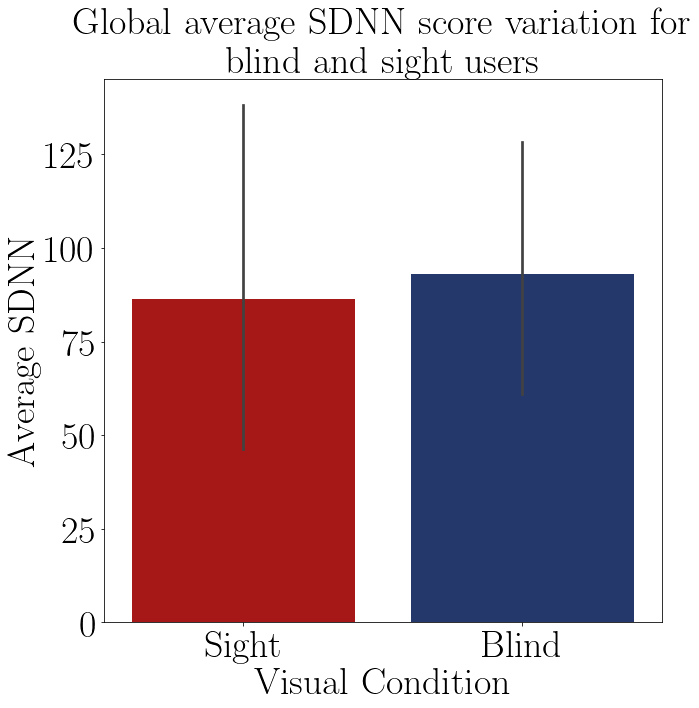
\includegraphics[width = \linewidth]{Resultados/ECG/Figuras/png/barplot_ecg_sdnn_global.png}
        %\resizebox{0.6\linewidth}{!}{
        %%% Creator: Matplotlib, PGF backend
%%
%% To include the figure in your LaTeX document, write
%%   \input{<filename>.pgf}
%%
%% Make sure the required packages are loaded in your preamble
%%   \usepackage{pgf}
%%
%% Figures using additional raster images can only be included by \input if
%% they are in the same directory as the main LaTeX file. For loading figures
%% from other directories you can use the `import` package
%%   \usepackage{import}
%%
%% and then include the figures with
%%   \import{<path to file>}{<filename>.pgf}
%%
%% Matplotlib used the following preamble
%%   \usepackage{fontspec}
%%
\begingroup%
\makeatletter%
\begin{pgfpicture}%
\pgfpathrectangle{\pgfpointorigin}{\pgfqpoint{8.990505in}{9.874752in}}%
\pgfusepath{use as bounding box, clip}%
\begin{pgfscope}%
\pgfsetbuttcap%
\pgfsetmiterjoin%
\pgfsetlinewidth{0.000000pt}%
\definecolor{currentstroke}{rgb}{1.000000,1.000000,1.000000}%
\pgfsetstrokecolor{currentstroke}%
\pgfsetstrokeopacity{0.000000}%
\pgfsetdash{}{0pt}%
\pgfpathmoveto{\pgfqpoint{0.000000in}{0.000000in}}%
\pgfpathlineto{\pgfqpoint{8.990505in}{0.000000in}}%
\pgfpathlineto{\pgfqpoint{8.990505in}{9.874752in}}%
\pgfpathlineto{\pgfqpoint{0.000000in}{9.874752in}}%
\pgfpathclose%
\pgfusepath{}%
\end{pgfscope}%
\begin{pgfscope}%
\pgfsetbuttcap%
\pgfsetmiterjoin%
\definecolor{currentfill}{rgb}{1.000000,1.000000,1.000000}%
\pgfsetfillcolor{currentfill}%
\pgfsetlinewidth{0.000000pt}%
\definecolor{currentstroke}{rgb}{0.000000,0.000000,0.000000}%
\pgfsetstrokecolor{currentstroke}%
\pgfsetstrokeopacity{0.000000}%
\pgfsetdash{}{0pt}%
\pgfpathmoveto{\pgfqpoint{1.140505in}{1.198954in}}%
\pgfpathlineto{\pgfqpoint{8.890505in}{1.198954in}}%
\pgfpathlineto{\pgfqpoint{8.890505in}{8.748954in}}%
\pgfpathlineto{\pgfqpoint{1.140505in}{8.748954in}}%
\pgfpathclose%
\pgfusepath{fill}%
\end{pgfscope}%
\begin{pgfscope}%
\pgfpathrectangle{\pgfqpoint{1.140505in}{1.198954in}}{\pgfqpoint{7.750000in}{7.550000in}}%
\pgfusepath{clip}%
\pgfsetbuttcap%
\pgfsetmiterjoin%
\definecolor{currentfill}{rgb}{0.651961,0.093137,0.093137}%
\pgfsetfillcolor{currentfill}%
\pgfsetlinewidth{0.000000pt}%
\definecolor{currentstroke}{rgb}{0.000000,0.000000,0.000000}%
\pgfsetstrokecolor{currentstroke}%
\pgfsetstrokeopacity{0.000000}%
\pgfsetdash{}{0pt}%
\pgfpathmoveto{\pgfqpoint{1.528005in}{1.198954in}}%
\pgfpathlineto{\pgfqpoint{4.628005in}{1.198954in}}%
\pgfpathlineto{\pgfqpoint{4.628005in}{6.762738in}}%
\pgfpathlineto{\pgfqpoint{1.528005in}{6.762738in}}%
\pgfpathclose%
\pgfusepath{fill}%
\end{pgfscope}%
\begin{pgfscope}%
\pgfpathrectangle{\pgfqpoint{1.140505in}{1.198954in}}{\pgfqpoint{7.750000in}{7.550000in}}%
\pgfusepath{clip}%
\pgfsetbuttcap%
\pgfsetmiterjoin%
\definecolor{currentfill}{rgb}{0.144608,0.218137,0.424020}%
\pgfsetfillcolor{currentfill}%
\pgfsetlinewidth{0.000000pt}%
\definecolor{currentstroke}{rgb}{0.000000,0.000000,0.000000}%
\pgfsetstrokecolor{currentstroke}%
\pgfsetstrokeopacity{0.000000}%
\pgfsetdash{}{0pt}%
\pgfpathmoveto{\pgfqpoint{5.403005in}{1.198954in}}%
\pgfpathlineto{\pgfqpoint{8.503005in}{1.198954in}}%
\pgfpathlineto{\pgfqpoint{8.503005in}{7.732572in}}%
\pgfpathlineto{\pgfqpoint{5.403005in}{7.732572in}}%
\pgfpathclose%
\pgfusepath{fill}%
\end{pgfscope}%
\begin{pgfscope}%
\pgfsetbuttcap%
\pgfsetroundjoin%
\definecolor{currentfill}{rgb}{0.000000,0.000000,0.000000}%
\pgfsetfillcolor{currentfill}%
\pgfsetlinewidth{0.803000pt}%
\definecolor{currentstroke}{rgb}{0.000000,0.000000,0.000000}%
\pgfsetstrokecolor{currentstroke}%
\pgfsetdash{}{0pt}%
\pgfsys@defobject{currentmarker}{\pgfqpoint{0.000000in}{-0.048611in}}{\pgfqpoint{0.000000in}{0.000000in}}{%
\pgfpathmoveto{\pgfqpoint{0.000000in}{0.000000in}}%
\pgfpathlineto{\pgfqpoint{0.000000in}{-0.048611in}}%
\pgfusepath{stroke,fill}%
}%
\begin{pgfscope}%
\pgfsys@transformshift{3.078005in}{1.198954in}%
\pgfsys@useobject{currentmarker}{}%
\end{pgfscope}%
\end{pgfscope}%
\begin{pgfscope}%
\definecolor{textcolor}{rgb}{0.000000,0.000000,0.000000}%
\pgfsetstrokecolor{textcolor}%
\pgfsetfillcolor{textcolor}%
\pgftext[x=3.078005in,y=1.101732in,,top]{\color{textcolor}\rmfamily\fontsize{38.016000}{45.619200}\selectfont Sight}%
\end{pgfscope}%
\begin{pgfscope}%
\pgfsetbuttcap%
\pgfsetroundjoin%
\definecolor{currentfill}{rgb}{0.000000,0.000000,0.000000}%
\pgfsetfillcolor{currentfill}%
\pgfsetlinewidth{0.803000pt}%
\definecolor{currentstroke}{rgb}{0.000000,0.000000,0.000000}%
\pgfsetstrokecolor{currentstroke}%
\pgfsetdash{}{0pt}%
\pgfsys@defobject{currentmarker}{\pgfqpoint{0.000000in}{-0.048611in}}{\pgfqpoint{0.000000in}{0.000000in}}{%
\pgfpathmoveto{\pgfqpoint{0.000000in}{0.000000in}}%
\pgfpathlineto{\pgfqpoint{0.000000in}{-0.048611in}}%
\pgfusepath{stroke,fill}%
}%
\begin{pgfscope}%
\pgfsys@transformshift{6.953005in}{1.198954in}%
\pgfsys@useobject{currentmarker}{}%
\end{pgfscope}%
\end{pgfscope}%
\begin{pgfscope}%
\definecolor{textcolor}{rgb}{0.000000,0.000000,0.000000}%
\pgfsetstrokecolor{textcolor}%
\pgfsetfillcolor{textcolor}%
\pgftext[x=6.953005in,y=1.101732in,,top]{\color{textcolor}\rmfamily\fontsize{38.016000}{45.619200}\selectfont Blind}%
\end{pgfscope}%
\begin{pgfscope}%
\definecolor{textcolor}{rgb}{0.000000,0.000000,0.000000}%
\pgfsetstrokecolor{textcolor}%
\pgfsetfillcolor{textcolor}%
\pgftext[x=5.015505in,y=0.569392in,,top]{\color{textcolor}\rmfamily\fontsize{38.016000}{45.619200}\selectfont Visual Condition}%
\end{pgfscope}%
\begin{pgfscope}%
\pgfsetbuttcap%
\pgfsetroundjoin%
\definecolor{currentfill}{rgb}{0.000000,0.000000,0.000000}%
\pgfsetfillcolor{currentfill}%
\pgfsetlinewidth{0.803000pt}%
\definecolor{currentstroke}{rgb}{0.000000,0.000000,0.000000}%
\pgfsetstrokecolor{currentstroke}%
\pgfsetdash{}{0pt}%
\pgfsys@defobject{currentmarker}{\pgfqpoint{-0.048611in}{0.000000in}}{\pgfqpoint{-0.000000in}{0.000000in}}{%
\pgfpathmoveto{\pgfqpoint{-0.000000in}{0.000000in}}%
\pgfpathlineto{\pgfqpoint{-0.048611in}{0.000000in}}%
\pgfusepath{stroke,fill}%
}%
\begin{pgfscope}%
\pgfsys@transformshift{1.140505in}{1.198954in}%
\pgfsys@useobject{currentmarker}{}%
\end{pgfscope}%
\end{pgfscope}%
\begin{pgfscope}%
\definecolor{textcolor}{rgb}{0.000000,0.000000,0.000000}%
\pgfsetstrokecolor{textcolor}%
\pgfsetfillcolor{textcolor}%
\pgftext[x=0.632340in, y=1.015738in, left, base]{\color{textcolor}\rmfamily\fontsize{38.016000}{45.619200}\selectfont \(\displaystyle {0.0}\)}%
\end{pgfscope}%
\begin{pgfscope}%
\pgfsetbuttcap%
\pgfsetroundjoin%
\definecolor{currentfill}{rgb}{0.000000,0.000000,0.000000}%
\pgfsetfillcolor{currentfill}%
\pgfsetlinewidth{0.803000pt}%
\definecolor{currentstroke}{rgb}{0.000000,0.000000,0.000000}%
\pgfsetstrokecolor{currentstroke}%
\pgfsetdash{}{0pt}%
\pgfsys@defobject{currentmarker}{\pgfqpoint{-0.048611in}{0.000000in}}{\pgfqpoint{-0.000000in}{0.000000in}}{%
\pgfpathmoveto{\pgfqpoint{-0.000000in}{0.000000in}}%
\pgfpathlineto{\pgfqpoint{-0.048611in}{0.000000in}}%
\pgfusepath{stroke,fill}%
}%
\begin{pgfscope}%
\pgfsys@transformshift{1.140505in}{3.178838in}%
\pgfsys@useobject{currentmarker}{}%
\end{pgfscope}%
\end{pgfscope}%
\begin{pgfscope}%
\definecolor{textcolor}{rgb}{0.000000,0.000000,0.000000}%
\pgfsetstrokecolor{textcolor}%
\pgfsetfillcolor{textcolor}%
\pgftext[x=0.632340in, y=2.995622in, left, base]{\color{textcolor}\rmfamily\fontsize{38.016000}{45.619200}\selectfont \(\displaystyle {0.2}\)}%
\end{pgfscope}%
\begin{pgfscope}%
\pgfsetbuttcap%
\pgfsetroundjoin%
\definecolor{currentfill}{rgb}{0.000000,0.000000,0.000000}%
\pgfsetfillcolor{currentfill}%
\pgfsetlinewidth{0.803000pt}%
\definecolor{currentstroke}{rgb}{0.000000,0.000000,0.000000}%
\pgfsetstrokecolor{currentstroke}%
\pgfsetdash{}{0pt}%
\pgfsys@defobject{currentmarker}{\pgfqpoint{-0.048611in}{0.000000in}}{\pgfqpoint{-0.000000in}{0.000000in}}{%
\pgfpathmoveto{\pgfqpoint{-0.000000in}{0.000000in}}%
\pgfpathlineto{\pgfqpoint{-0.048611in}{0.000000in}}%
\pgfusepath{stroke,fill}%
}%
\begin{pgfscope}%
\pgfsys@transformshift{1.140505in}{5.158723in}%
\pgfsys@useobject{currentmarker}{}%
\end{pgfscope}%
\end{pgfscope}%
\begin{pgfscope}%
\definecolor{textcolor}{rgb}{0.000000,0.000000,0.000000}%
\pgfsetstrokecolor{textcolor}%
\pgfsetfillcolor{textcolor}%
\pgftext[x=0.632340in, y=4.975506in, left, base]{\color{textcolor}\rmfamily\fontsize{38.016000}{45.619200}\selectfont \(\displaystyle {0.4}\)}%
\end{pgfscope}%
\begin{pgfscope}%
\pgfsetbuttcap%
\pgfsetroundjoin%
\definecolor{currentfill}{rgb}{0.000000,0.000000,0.000000}%
\pgfsetfillcolor{currentfill}%
\pgfsetlinewidth{0.803000pt}%
\definecolor{currentstroke}{rgb}{0.000000,0.000000,0.000000}%
\pgfsetstrokecolor{currentstroke}%
\pgfsetdash{}{0pt}%
\pgfsys@defobject{currentmarker}{\pgfqpoint{-0.048611in}{0.000000in}}{\pgfqpoint{-0.000000in}{0.000000in}}{%
\pgfpathmoveto{\pgfqpoint{-0.000000in}{0.000000in}}%
\pgfpathlineto{\pgfqpoint{-0.048611in}{0.000000in}}%
\pgfusepath{stroke,fill}%
}%
\begin{pgfscope}%
\pgfsys@transformshift{1.140505in}{7.138607in}%
\pgfsys@useobject{currentmarker}{}%
\end{pgfscope}%
\end{pgfscope}%
\begin{pgfscope}%
\definecolor{textcolor}{rgb}{0.000000,0.000000,0.000000}%
\pgfsetstrokecolor{textcolor}%
\pgfsetfillcolor{textcolor}%
\pgftext[x=0.632340in, y=6.955391in, left, base]{\color{textcolor}\rmfamily\fontsize{38.016000}{45.619200}\selectfont \(\displaystyle {0.6}\)}%
\end{pgfscope}%
\begin{pgfscope}%
\definecolor{textcolor}{rgb}{0.000000,0.000000,0.000000}%
\pgfsetstrokecolor{textcolor}%
\pgfsetfillcolor{textcolor}%
\pgftext[x=0.576784in,y=4.973954in,,bottom,rotate=90.000000]{\color{textcolor}\rmfamily\fontsize{38.016000}{45.619200}\selectfont Sagat score average}%
\end{pgfscope}%
\begin{pgfscope}%
\pgfpathrectangle{\pgfqpoint{1.140505in}{1.198954in}}{\pgfqpoint{7.750000in}{7.550000in}}%
\pgfusepath{clip}%
\pgfsetrectcap%
\pgfsetroundjoin%
\pgfsetlinewidth{2.710125pt}%
\definecolor{currentstroke}{rgb}{0.260000,0.260000,0.260000}%
\pgfsetstrokecolor{currentstroke}%
\pgfsetdash{}{0pt}%
\pgfpathmoveto{\pgfqpoint{3.078005in}{6.090776in}}%
\pgfpathlineto{\pgfqpoint{3.078005in}{7.385195in}}%
\pgfusepath{stroke}%
\end{pgfscope}%
\begin{pgfscope}%
\pgfpathrectangle{\pgfqpoint{1.140505in}{1.198954in}}{\pgfqpoint{7.750000in}{7.550000in}}%
\pgfusepath{clip}%
\pgfsetrectcap%
\pgfsetroundjoin%
\pgfsetlinewidth{2.710125pt}%
\definecolor{currentstroke}{rgb}{0.260000,0.260000,0.260000}%
\pgfsetstrokecolor{currentstroke}%
\pgfsetdash{}{0pt}%
\pgfpathmoveto{\pgfqpoint{6.953005in}{7.125552in}}%
\pgfpathlineto{\pgfqpoint{6.953005in}{8.389430in}}%
\pgfusepath{stroke}%
\end{pgfscope}%
\begin{pgfscope}%
\pgfsetrectcap%
\pgfsetmiterjoin%
\pgfsetlinewidth{0.803000pt}%
\definecolor{currentstroke}{rgb}{0.000000,0.000000,0.000000}%
\pgfsetstrokecolor{currentstroke}%
\pgfsetdash{}{0pt}%
\pgfpathmoveto{\pgfqpoint{1.140505in}{1.198954in}}%
\pgfpathlineto{\pgfqpoint{1.140505in}{8.748954in}}%
\pgfusepath{stroke}%
\end{pgfscope}%
\begin{pgfscope}%
\pgfsetrectcap%
\pgfsetmiterjoin%
\pgfsetlinewidth{0.803000pt}%
\definecolor{currentstroke}{rgb}{0.000000,0.000000,0.000000}%
\pgfsetstrokecolor{currentstroke}%
\pgfsetdash{}{0pt}%
\pgfpathmoveto{\pgfqpoint{8.890505in}{1.198954in}}%
\pgfpathlineto{\pgfqpoint{8.890505in}{8.748954in}}%
\pgfusepath{stroke}%
\end{pgfscope}%
\begin{pgfscope}%
\pgfsetrectcap%
\pgfsetmiterjoin%
\pgfsetlinewidth{0.803000pt}%
\definecolor{currentstroke}{rgb}{0.000000,0.000000,0.000000}%
\pgfsetstrokecolor{currentstroke}%
\pgfsetdash{}{0pt}%
\pgfpathmoveto{\pgfqpoint{1.140505in}{1.198954in}}%
\pgfpathlineto{\pgfqpoint{8.890505in}{1.198954in}}%
\pgfusepath{stroke}%
\end{pgfscope}%
\begin{pgfscope}%
\pgfsetrectcap%
\pgfsetmiterjoin%
\pgfsetlinewidth{0.803000pt}%
\definecolor{currentstroke}{rgb}{0.000000,0.000000,0.000000}%
\pgfsetstrokecolor{currentstroke}%
\pgfsetdash{}{0pt}%
\pgfpathmoveto{\pgfqpoint{1.140505in}{8.748954in}}%
\pgfpathlineto{\pgfqpoint{8.890505in}{8.748954in}}%
\pgfusepath{stroke}%
\end{pgfscope}%
\begin{pgfscope}%
\definecolor{textcolor}{rgb}{0.000000,0.000000,0.000000}%
\pgfsetstrokecolor{textcolor}%
\pgfsetfillcolor{textcolor}%
\pgftext[x=1.767248in, y=9.404096in, left, base]{\color{textcolor}\rmfamily\fontsize{38.016000}{45.619200}\selectfont Global sagat score average for }%
\end{pgfscope}%
\begin{pgfscope}%
\definecolor{textcolor}{rgb}{0.000000,0.000000,0.000000}%
\pgfsetstrokecolor{textcolor}%
\pgfsetfillcolor{textcolor}%
\pgftext[x=2.820080in, y=8.856666in, left, base]{\color{textcolor}\rmfamily\fontsize{38.016000}{45.619200}\selectfont   blind and sight users}%
\end{pgfscope}%
\end{pgfpicture}%
\makeatother%
\endgroup%

        %}
        \caption{Barplot of the average SDNN score of each group.}
        \label{fig:barplot_ecg_sdnn_global}
    \end{minipage}
\end{figure}


The Table \ref{tab:ecg_sdnn_average_group} shows the variation of the heartbeat in each round of each group. In general, all the standard deviations increased, meaning that the mental workload decreased between the "Baseline" and the method.


\begin{table}[!htb]
\centering
\caption{ECG Average SDNN average in relation to the baseline grouped by participant and visual Condition.}
\label{tab:ecg_sdnn_average_group}
\begin{tabular}{lrrrrr}
\toprule
{} &   Base &  Audio & Haptic Belt & Virtual Cane & Mixture \\
Visual Condition &        &        &             &              &         \\
\midrule
Blind            &  84.4% &  92.1% &       74.3% &       102.1% &  112.2% \\
Sight            &  29.3% &  43.2% &      152.0% &        92.9% &  114.7% \\
\bottomrule
\end{tabular}
\end{table}



The Shapiro–Wilk normality test on the Table \ref{tab:shapiro_ecg_sdnn} shows that all of the "blind" sample data are normally distributed, except the "Mixture" method. In the "sight" sample only the "Base" and the "Audio" method are normally distributed. That means that the following analyses cannot be made with those exceptions.

According to the T-Test presented in the Table \ref{tab:ttest_ecg_bpm} there is no difference in the heart rate frequency variation between the sample groups.

\begin{table}[!htb]
    \begin{minipage}{.45\linewidth}
        
\centering
\caption{Shapiro test p-value for the ecg average SDNN for each method and visual condition}
\label{tab:shapiro_ecg_sdnn}
\begin{tabular}{lr}
\toprule
            Method &  Shapiro P-Value \\
\midrule
        Base blind &            0.078 \\
        Base sight &            0.347 \\
       Audio blind &            0.071 \\
       Audio sight &            0.130 \\
 Haptic Belt blind &            0.414 \\
 Haptic Belt sight &            0.001 \\
Virtual Cane blind &            0.723 \\
Virtual Cane sight &            0.015 \\
     Mixture blind &            0.027 \\
     Mixture sight &            0.001 \\
\bottomrule
\end{tabular}

    \end{minipage}
    \hfill
    \begin{minipage}{.45\linewidth}
        \vspace{-2.75cm}
        
\centering
\caption{T test p-value for the ecg average SDNN each method for blinded users versus sighted users.}
\label{tab:ttest_ecg_sdnn}
\begin{tabular}{lr}
\toprule
      Method &  T-Test P-Value \\
\midrule
        Base &           0.230 \\
       Audio &           0.317 \\
 Haptic Belt &           0.434 \\
Virtual Cane &           0.862 \\
     Mixture &           0.976 \\
\bottomrule
\end{tabular}

    \end{minipage}
\end{table}

The Table \ref{tab:blocdanova_sdnn} shows the Anova test p-value of the heart rate frequency of the "blind" sample between the guidance methods presented in the Table \ref{tab:ecg_sdnn_table}. The p-value indicates that there is at least one method that is statistically equal to one of the other methods.


\begin{table}[!htb]
\centering
\caption{Anova p-value for the SDNN on each method for blinded users.}
\label{tab:blocdanova_sdnn}
\begin{tabular}{lrrrrr}
\toprule
               Source &  Squared sum &  DOF & Squared average &       F & \begin{tabular}[c]{@{}l@{}}P-Value \\ $(F_{0} > F)$\end{tabular} \\
\midrule
Participants (blocks) &   214885.879 &    3 &         879.920 & 127.314 &                                                                  \\
               Method &     3519.680 &    4 &       71628.626 &   1.564 &                                                            0.247 \\
   Experimental error &     6751.365 &   12 &         562.614 &         &                                                                  \\
                Total &   225156.923 &   19 &                 &         &                                                                  \\
\bottomrule
\end{tabular}
\end{table}



The Table \ref{tab:lsd_sdnn} presents the conclusion of a pairwise Fisher LSD test of the blind heart rate frequency variation between all the guidance methods. The results show that the "Virtual cane" and the "Mixture" method differs from the "Base" method.


\begin{table}[!htb]
\centering
\caption{Cross validation p-value for the average SDNN on each method for blinded users.}
\label{tab:lsd_sdnn}
\begin{tabular}{rclr}
\toprule
      \multicolumn{3}{c}{Method} &                                           Analysis \\
\midrule
              Base & $X$ & Audio &                   $H_0 : \mu_{Base} = \mu_{Audio}$ \\
        Base & $X$ & Haptic Belt &             $H_0 : \mu_{Base} = \mu_{Haptic Belt}$ \\
       Base & $X$ & Virtual Cane &        $H_1 : \mu_{Base} \ne \mu_{Virtual Cane}**$ \\
            Base & $X$ & Mixture &             $H_1 : \mu_{Base} \ne \mu_{Mixture}**$ \\
       Audio & $X$ & Haptic Belt &        $H_1 : \mu_{Audio} \ne \mu_{Haptic Belt}**$ \\
      Audio & $X$ & Virtual Cane &           $H_0 : \mu_{Audio} = \mu_{Virtual Cane}$ \\
           Audio & $X$ & Mixture &            $H_1 : \mu_{Audio} \ne \mu_{Mixture}**$ \\
Haptic Belt & $X$ & Virtual Cane & $H_1 : \mu_{Haptic Belt} \ne \mu_{Virtual Cane}**$ \\
     Haptic Belt & $X$ & Mixture &      $H_1 : \mu_{Haptic Belt} \ne \mu_{Mixture}**$ \\
    Virtual Cane & $X$ & Mixture &         $H_0 : \mu_{Virtual Cane} = \mu_{Mixture}$ \\
\bottomrule
\end{tabular}
\end{table}



According to the Anova test at Table \ref{tab:blocdanova_sdnn} and the LSD test at \ref{tab:lsd_sdnn} and the Table \ref{tab:ecg_sdnn_average_group} the "Virtual cane" and the "Mixture" method did provoke an increase in the heartrate variancy.

\FloatBarrier

\subsection{Galvanic skin reaction and temperature data;}
\label{subsec:results_gsr_temp}

The GSR analysis is made by analyzing the average in each round and comparing it with the "Baseline" average. The temperature was analyzed with the GSR to see if there is some influence and by a graphical analysis there was none.

\subsubsection{Analysis of the GSR average}

The Table \ref{tab:gsr_avg_table} presents the average skin conductance by each participant on each scenes and they are plotted in the Figures \ref{fig:barplot_gsr_scene_blind} and \ref{fig:barplot_gsr_scene_sight}. It is possible to see that in all of the methods there was an increase in the average skin conductance, meaning that the user was aroused and maybe an increase in the mental workload.

%
\begin{table}[!htb]
\centering
\caption{Average GSR felled by the participants.}
\label{tab:gsr_avg_table}
\begin{tabular}{lllrrrrrr}
\toprule
    &       &        & Baseline &   Base &  Audio & \begin{tabular}[c]{@{}l@{}}Haptic\\ Belt\end{tabular} & \begin{tabular}[c]{@{}l@{}}Virtual\\ Cane\end{tabular} & Mixture \\
Participant & Visual Condition & Round &          &        &        &                                                       &                                                        &         \\
\midrule
001 & Sight & First &     4.27 &   8.80 &  15.19 &                                                 15.67 &                                                  15.19 &   14.15 \\
    &       & Return &          &  11.48 &  14.95 &                                                 15.09 &                                                  15.72 &   21.52 \\
001C & Blind & First &     0.37 &   0.48 &   1.03 &                                                  3.14 &                                                   3.79 &    3.90 \\
    &       & Return &          &   0.83 &   1.58 &                                                  2.81 &                                                   4.04 &    4.57 \\
002C & Blind & First &     0.17 &   0.91 &   0.23 &                                                  0.17 &                                                   0.17 &    0.17 \\
    &       & Return &          &   0.43 &   0.17 &                                                  0.16 &                                                   0.17 &    0.17 \\
003 & Sight & First &     0.19 &   0.19 &   0.17 &                                                  0.17 &                                                   0.17 &    0.17 \\
    &       & Return &          &   0.17 &   0.17 &                                                  0.17 &                                                   0.17 &    0.17 \\
003C & Blind & First &     0.30 &   0.56 &   0.56 &                                                  0.62 &                                                   0.85 &    1.09 \\
    &       & Return &          &   0.62 &   0.63 &                                                  0.65 &                                                   0.92 &    1.06 \\
004 & Sight & First &     2.60 &   9.71 &  11.18 &                                                 12.60 &                                                  12.92 &   10.34 \\
    &       & Return &          &  10.89 &  11.97 &                                                 12.25 &                                                  13.47 &   10.16 \\
004C & Blind & First &     1.24 &   2.34 &   3.07 &                                                  3.49 &                                                   2.28 &    2.23 \\
    &       & Return &          &   2.57 &   2.95 &                                                  3.20 &                                                   2.21 &    2.24 \\
005 & Sight & First &     0.47 &   1.88 &   1.58 &                                                  1.44 &                                                   1.37 &    1.33 \\
    &       & Return &          &   1.66 &   1.53 &                                                  1.47 &                                                   1.49 &    1.33 \\
\bottomrule
\end{tabular}
\end{table}



%\begin{figure}[!htb]
%    \centering
%    \begin{minipage}{\textwidth}
%        \centering
%        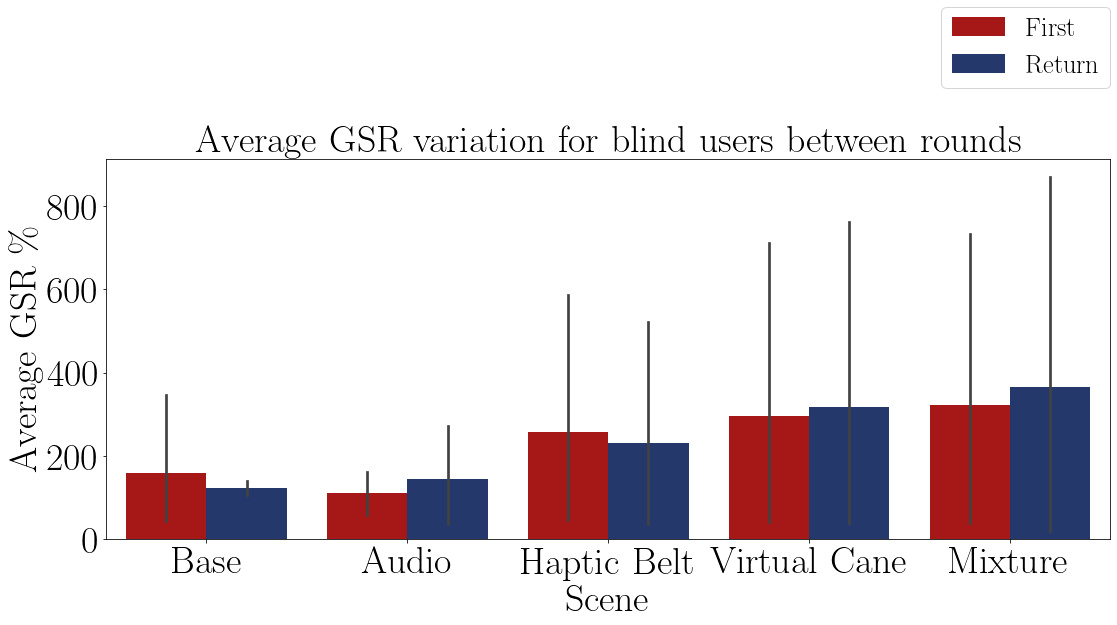
\includegraphics[width = 0.8\linewidth]{Resultados/GSR/Figuras/png/barplot_gsr_avg_scene_blind.png}
%        %\resizebox{0.8\linewidth}{!}{
%        %%% Creator: Matplotlib, PGF backend
%%
%% To include the figure in your LaTeX document, write
%%   \input{<filename>.pgf}
%%
%% Make sure the required packages are loaded in your preamble
%%   \usepackage{pgf}
%%
%% Figures using additional raster images can only be included by \input if
%% they are in the same directory as the main LaTeX file. For loading figures
%% from other directories you can use the `import` package
%%   \usepackage{import}
%%
%% and then include the figures with
%%   \import{<path to file>}{<filename>.pgf}
%%
%% Matplotlib used the following preamble
%%   \usepackage{fontspec}
%%
\begingroup%
\makeatletter%
\begin{pgfpicture}%
\pgfpathrectangle{\pgfpointorigin}{\pgfqpoint{15.369508in}{8.690562in}}%
\pgfusepath{use as bounding box, clip}%
\begin{pgfscope}%
\pgfsetbuttcap%
\pgfsetmiterjoin%
\pgfsetlinewidth{0.000000pt}%
\definecolor{currentstroke}{rgb}{1.000000,1.000000,1.000000}%
\pgfsetstrokecolor{currentstroke}%
\pgfsetstrokeopacity{0.000000}%
\pgfsetdash{}{0pt}%
\pgfpathmoveto{\pgfqpoint{0.000000in}{-0.000000in}}%
\pgfpathlineto{\pgfqpoint{15.369508in}{-0.000000in}}%
\pgfpathlineto{\pgfqpoint{15.369508in}{8.690562in}}%
\pgfpathlineto{\pgfqpoint{0.000000in}{8.690562in}}%
\pgfpathclose%
\pgfusepath{}%
\end{pgfscope}%
\begin{pgfscope}%
\pgfsetbuttcap%
\pgfsetmiterjoin%
\definecolor{currentfill}{rgb}{1.000000,1.000000,1.000000}%
\pgfsetfillcolor{currentfill}%
\pgfsetlinewidth{0.000000pt}%
\definecolor{currentstroke}{rgb}{0.000000,0.000000,0.000000}%
\pgfsetstrokecolor{currentstroke}%
\pgfsetstrokeopacity{0.000000}%
\pgfsetdash{}{0pt}%
\pgfpathmoveto{\pgfqpoint{1.319508in}{1.191562in}}%
\pgfpathlineto{\pgfqpoint{15.269508in}{1.191562in}}%
\pgfpathlineto{\pgfqpoint{15.269508in}{6.476562in}}%
\pgfpathlineto{\pgfqpoint{1.319508in}{6.476562in}}%
\pgfpathclose%
\pgfusepath{fill}%
\end{pgfscope}%
\begin{pgfscope}%
\pgfpathrectangle{\pgfqpoint{1.319508in}{1.191562in}}{\pgfqpoint{13.950000in}{5.285000in}}%
\pgfusepath{clip}%
\pgfsetbuttcap%
\pgfsetmiterjoin%
\definecolor{currentfill}{rgb}{0.651961,0.093137,0.093137}%
\pgfsetfillcolor{currentfill}%
\pgfsetlinewidth{0.000000pt}%
\definecolor{currentstroke}{rgb}{0.000000,0.000000,0.000000}%
\pgfsetstrokecolor{currentstroke}%
\pgfsetstrokeopacity{0.000000}%
\pgfsetdash{}{0pt}%
\pgfpathmoveto{\pgfqpoint{1.598508in}{5.432025in}}%
\pgfpathlineto{\pgfqpoint{2.714508in}{5.432025in}}%
\pgfpathlineto{\pgfqpoint{2.714508in}{4.583309in}}%
\pgfpathlineto{\pgfqpoint{1.598508in}{4.583309in}}%
\pgfpathclose%
\pgfusepath{fill}%
\end{pgfscope}%
\begin{pgfscope}%
\pgfpathrectangle{\pgfqpoint{1.319508in}{1.191562in}}{\pgfqpoint{13.950000in}{5.285000in}}%
\pgfusepath{clip}%
\pgfsetbuttcap%
\pgfsetmiterjoin%
\definecolor{currentfill}{rgb}{0.651961,0.093137,0.093137}%
\pgfsetfillcolor{currentfill}%
\pgfsetlinewidth{0.000000pt}%
\definecolor{currentstroke}{rgb}{0.000000,0.000000,0.000000}%
\pgfsetstrokecolor{currentstroke}%
\pgfsetstrokeopacity{0.000000}%
\pgfsetdash{}{0pt}%
\pgfpathmoveto{\pgfqpoint{4.388508in}{5.432025in}}%
\pgfpathlineto{\pgfqpoint{5.504508in}{5.432025in}}%
\pgfpathlineto{\pgfqpoint{5.504508in}{3.558465in}}%
\pgfpathlineto{\pgfqpoint{4.388508in}{3.558465in}}%
\pgfpathclose%
\pgfusepath{fill}%
\end{pgfscope}%
\begin{pgfscope}%
\pgfpathrectangle{\pgfqpoint{1.319508in}{1.191562in}}{\pgfqpoint{13.950000in}{5.285000in}}%
\pgfusepath{clip}%
\pgfsetbuttcap%
\pgfsetmiterjoin%
\definecolor{currentfill}{rgb}{0.651961,0.093137,0.093137}%
\pgfsetfillcolor{currentfill}%
\pgfsetlinewidth{0.000000pt}%
\definecolor{currentstroke}{rgb}{0.000000,0.000000,0.000000}%
\pgfsetstrokecolor{currentstroke}%
\pgfsetstrokeopacity{0.000000}%
\pgfsetdash{}{0pt}%
\pgfpathmoveto{\pgfqpoint{7.178508in}{5.432025in}}%
\pgfpathlineto{\pgfqpoint{8.294508in}{5.432025in}}%
\pgfpathlineto{\pgfqpoint{8.294508in}{4.476572in}}%
\pgfpathlineto{\pgfqpoint{7.178508in}{4.476572in}}%
\pgfpathclose%
\pgfusepath{fill}%
\end{pgfscope}%
\begin{pgfscope}%
\pgfpathrectangle{\pgfqpoint{1.319508in}{1.191562in}}{\pgfqpoint{13.950000in}{5.285000in}}%
\pgfusepath{clip}%
\pgfsetbuttcap%
\pgfsetmiterjoin%
\definecolor{currentfill}{rgb}{0.651961,0.093137,0.093137}%
\pgfsetfillcolor{currentfill}%
\pgfsetlinewidth{0.000000pt}%
\definecolor{currentstroke}{rgb}{0.000000,0.000000,0.000000}%
\pgfsetstrokecolor{currentstroke}%
\pgfsetstrokeopacity{0.000000}%
\pgfsetdash{}{0pt}%
\pgfpathmoveto{\pgfqpoint{9.968508in}{5.432025in}}%
\pgfpathlineto{\pgfqpoint{11.084508in}{5.432025in}}%
\pgfpathlineto{\pgfqpoint{11.084508in}{3.778608in}}%
\pgfpathlineto{\pgfqpoint{9.968508in}{3.778608in}}%
\pgfpathclose%
\pgfusepath{fill}%
\end{pgfscope}%
\begin{pgfscope}%
\pgfpathrectangle{\pgfqpoint{1.319508in}{1.191562in}}{\pgfqpoint{13.950000in}{5.285000in}}%
\pgfusepath{clip}%
\pgfsetbuttcap%
\pgfsetmiterjoin%
\definecolor{currentfill}{rgb}{0.651961,0.093137,0.093137}%
\pgfsetfillcolor{currentfill}%
\pgfsetlinewidth{0.000000pt}%
\definecolor{currentstroke}{rgb}{0.000000,0.000000,0.000000}%
\pgfsetstrokecolor{currentstroke}%
\pgfsetstrokeopacity{0.000000}%
\pgfsetdash{}{0pt}%
\pgfpathmoveto{\pgfqpoint{12.758508in}{5.432025in}}%
\pgfpathlineto{\pgfqpoint{13.874508in}{5.432025in}}%
\pgfpathlineto{\pgfqpoint{13.874508in}{4.339698in}}%
\pgfpathlineto{\pgfqpoint{12.758508in}{4.339698in}}%
\pgfpathclose%
\pgfusepath{fill}%
\end{pgfscope}%
\begin{pgfscope}%
\pgfpathrectangle{\pgfqpoint{1.319508in}{1.191562in}}{\pgfqpoint{13.950000in}{5.285000in}}%
\pgfusepath{clip}%
\pgfsetbuttcap%
\pgfsetmiterjoin%
\definecolor{currentfill}{rgb}{0.144608,0.218137,0.424020}%
\pgfsetfillcolor{currentfill}%
\pgfsetlinewidth{0.000000pt}%
\definecolor{currentstroke}{rgb}{0.000000,0.000000,0.000000}%
\pgfsetstrokecolor{currentstroke}%
\pgfsetstrokeopacity{0.000000}%
\pgfsetdash{}{0pt}%
\pgfpathmoveto{\pgfqpoint{2.714508in}{5.432025in}}%
\pgfpathlineto{\pgfqpoint{3.830508in}{5.432025in}}%
\pgfpathlineto{\pgfqpoint{3.830508in}{4.506389in}}%
\pgfpathlineto{\pgfqpoint{2.714508in}{4.506389in}}%
\pgfpathclose%
\pgfusepath{fill}%
\end{pgfscope}%
\begin{pgfscope}%
\pgfpathrectangle{\pgfqpoint{1.319508in}{1.191562in}}{\pgfqpoint{13.950000in}{5.285000in}}%
\pgfusepath{clip}%
\pgfsetbuttcap%
\pgfsetmiterjoin%
\definecolor{currentfill}{rgb}{0.144608,0.218137,0.424020}%
\pgfsetfillcolor{currentfill}%
\pgfsetlinewidth{0.000000pt}%
\definecolor{currentstroke}{rgb}{0.000000,0.000000,0.000000}%
\pgfsetstrokecolor{currentstroke}%
\pgfsetstrokeopacity{0.000000}%
\pgfsetdash{}{0pt}%
\pgfpathmoveto{\pgfqpoint{5.504508in}{5.432025in}}%
\pgfpathlineto{\pgfqpoint{6.620508in}{5.432025in}}%
\pgfpathlineto{\pgfqpoint{6.620508in}{3.808164in}}%
\pgfpathlineto{\pgfqpoint{5.504508in}{3.808164in}}%
\pgfpathclose%
\pgfusepath{fill}%
\end{pgfscope}%
\begin{pgfscope}%
\pgfpathrectangle{\pgfqpoint{1.319508in}{1.191562in}}{\pgfqpoint{13.950000in}{5.285000in}}%
\pgfusepath{clip}%
\pgfsetbuttcap%
\pgfsetmiterjoin%
\definecolor{currentfill}{rgb}{0.144608,0.218137,0.424020}%
\pgfsetfillcolor{currentfill}%
\pgfsetlinewidth{0.000000pt}%
\definecolor{currentstroke}{rgb}{0.000000,0.000000,0.000000}%
\pgfsetstrokecolor{currentstroke}%
\pgfsetstrokeopacity{0.000000}%
\pgfsetdash{}{0pt}%
\pgfpathmoveto{\pgfqpoint{8.294508in}{5.432025in}}%
\pgfpathlineto{\pgfqpoint{9.410508in}{5.432025in}}%
\pgfpathlineto{\pgfqpoint{9.410508in}{4.696413in}}%
\pgfpathlineto{\pgfqpoint{8.294508in}{4.696413in}}%
\pgfpathclose%
\pgfusepath{fill}%
\end{pgfscope}%
\begin{pgfscope}%
\pgfpathrectangle{\pgfqpoint{1.319508in}{1.191562in}}{\pgfqpoint{13.950000in}{5.285000in}}%
\pgfusepath{clip}%
\pgfsetbuttcap%
\pgfsetmiterjoin%
\definecolor{currentfill}{rgb}{0.144608,0.218137,0.424020}%
\pgfsetfillcolor{currentfill}%
\pgfsetlinewidth{0.000000pt}%
\definecolor{currentstroke}{rgb}{0.000000,0.000000,0.000000}%
\pgfsetstrokecolor{currentstroke}%
\pgfsetstrokeopacity{0.000000}%
\pgfsetdash{}{0pt}%
\pgfpathmoveto{\pgfqpoint{11.084508in}{5.432025in}}%
\pgfpathlineto{\pgfqpoint{12.200508in}{5.432025in}}%
\pgfpathlineto{\pgfqpoint{12.200508in}{4.423975in}}%
\pgfpathlineto{\pgfqpoint{11.084508in}{4.423975in}}%
\pgfpathclose%
\pgfusepath{fill}%
\end{pgfscope}%
\begin{pgfscope}%
\pgfpathrectangle{\pgfqpoint{1.319508in}{1.191562in}}{\pgfqpoint{13.950000in}{5.285000in}}%
\pgfusepath{clip}%
\pgfsetbuttcap%
\pgfsetmiterjoin%
\definecolor{currentfill}{rgb}{0.144608,0.218137,0.424020}%
\pgfsetfillcolor{currentfill}%
\pgfsetlinewidth{0.000000pt}%
\definecolor{currentstroke}{rgb}{0.000000,0.000000,0.000000}%
\pgfsetstrokecolor{currentstroke}%
\pgfsetstrokeopacity{0.000000}%
\pgfsetdash{}{0pt}%
\pgfpathmoveto{\pgfqpoint{13.874508in}{5.432025in}}%
\pgfpathlineto{\pgfqpoint{14.990508in}{5.432025in}}%
\pgfpathlineto{\pgfqpoint{14.990508in}{4.469000in}}%
\pgfpathlineto{\pgfqpoint{13.874508in}{4.469000in}}%
\pgfpathclose%
\pgfusepath{fill}%
\end{pgfscope}%
\begin{pgfscope}%
\pgfsetbuttcap%
\pgfsetroundjoin%
\definecolor{currentfill}{rgb}{0.000000,0.000000,0.000000}%
\pgfsetfillcolor{currentfill}%
\pgfsetlinewidth{0.803000pt}%
\definecolor{currentstroke}{rgb}{0.000000,0.000000,0.000000}%
\pgfsetstrokecolor{currentstroke}%
\pgfsetdash{}{0pt}%
\pgfsys@defobject{currentmarker}{\pgfqpoint{0.000000in}{-0.048611in}}{\pgfqpoint{0.000000in}{0.000000in}}{%
\pgfpathmoveto{\pgfqpoint{0.000000in}{0.000000in}}%
\pgfpathlineto{\pgfqpoint{0.000000in}{-0.048611in}}%
\pgfusepath{stroke,fill}%
}%
\begin{pgfscope}%
\pgfsys@transformshift{2.714508in}{1.191562in}%
\pgfsys@useobject{currentmarker}{}%
\end{pgfscope}%
\end{pgfscope}%
\begin{pgfscope}%
\definecolor{textcolor}{rgb}{0.000000,0.000000,0.000000}%
\pgfsetstrokecolor{textcolor}%
\pgfsetfillcolor{textcolor}%
\pgftext[x=2.714508in,y=1.094339in,,top]{\color{textcolor}\rmfamily\fontsize{38.016000}{45.619200}\selectfont Base}%
\end{pgfscope}%
\begin{pgfscope}%
\pgfsetbuttcap%
\pgfsetroundjoin%
\definecolor{currentfill}{rgb}{0.000000,0.000000,0.000000}%
\pgfsetfillcolor{currentfill}%
\pgfsetlinewidth{0.803000pt}%
\definecolor{currentstroke}{rgb}{0.000000,0.000000,0.000000}%
\pgfsetstrokecolor{currentstroke}%
\pgfsetdash{}{0pt}%
\pgfsys@defobject{currentmarker}{\pgfqpoint{0.000000in}{-0.048611in}}{\pgfqpoint{0.000000in}{0.000000in}}{%
\pgfpathmoveto{\pgfqpoint{0.000000in}{0.000000in}}%
\pgfpathlineto{\pgfqpoint{0.000000in}{-0.048611in}}%
\pgfusepath{stroke,fill}%
}%
\begin{pgfscope}%
\pgfsys@transformshift{5.504508in}{1.191562in}%
\pgfsys@useobject{currentmarker}{}%
\end{pgfscope}%
\end{pgfscope}%
\begin{pgfscope}%
\definecolor{textcolor}{rgb}{0.000000,0.000000,0.000000}%
\pgfsetstrokecolor{textcolor}%
\pgfsetfillcolor{textcolor}%
\pgftext[x=5.504508in,y=1.094339in,,top]{\color{textcolor}\rmfamily\fontsize{38.016000}{45.619200}\selectfont Audio}%
\end{pgfscope}%
\begin{pgfscope}%
\pgfsetbuttcap%
\pgfsetroundjoin%
\definecolor{currentfill}{rgb}{0.000000,0.000000,0.000000}%
\pgfsetfillcolor{currentfill}%
\pgfsetlinewidth{0.803000pt}%
\definecolor{currentstroke}{rgb}{0.000000,0.000000,0.000000}%
\pgfsetstrokecolor{currentstroke}%
\pgfsetdash{}{0pt}%
\pgfsys@defobject{currentmarker}{\pgfqpoint{0.000000in}{-0.048611in}}{\pgfqpoint{0.000000in}{0.000000in}}{%
\pgfpathmoveto{\pgfqpoint{0.000000in}{0.000000in}}%
\pgfpathlineto{\pgfqpoint{0.000000in}{-0.048611in}}%
\pgfusepath{stroke,fill}%
}%
\begin{pgfscope}%
\pgfsys@transformshift{8.294508in}{1.191562in}%
\pgfsys@useobject{currentmarker}{}%
\end{pgfscope}%
\end{pgfscope}%
\begin{pgfscope}%
\definecolor{textcolor}{rgb}{0.000000,0.000000,0.000000}%
\pgfsetstrokecolor{textcolor}%
\pgfsetfillcolor{textcolor}%
\pgftext[x=8.294508in,y=1.094339in,,top]{\color{textcolor}\rmfamily\fontsize{38.016000}{45.619200}\selectfont Haptic Belt}%
\end{pgfscope}%
\begin{pgfscope}%
\pgfsetbuttcap%
\pgfsetroundjoin%
\definecolor{currentfill}{rgb}{0.000000,0.000000,0.000000}%
\pgfsetfillcolor{currentfill}%
\pgfsetlinewidth{0.803000pt}%
\definecolor{currentstroke}{rgb}{0.000000,0.000000,0.000000}%
\pgfsetstrokecolor{currentstroke}%
\pgfsetdash{}{0pt}%
\pgfsys@defobject{currentmarker}{\pgfqpoint{0.000000in}{-0.048611in}}{\pgfqpoint{0.000000in}{0.000000in}}{%
\pgfpathmoveto{\pgfqpoint{0.000000in}{0.000000in}}%
\pgfpathlineto{\pgfqpoint{0.000000in}{-0.048611in}}%
\pgfusepath{stroke,fill}%
}%
\begin{pgfscope}%
\pgfsys@transformshift{11.084508in}{1.191562in}%
\pgfsys@useobject{currentmarker}{}%
\end{pgfscope}%
\end{pgfscope}%
\begin{pgfscope}%
\definecolor{textcolor}{rgb}{0.000000,0.000000,0.000000}%
\pgfsetstrokecolor{textcolor}%
\pgfsetfillcolor{textcolor}%
\pgftext[x=11.084508in,y=1.094339in,,top]{\color{textcolor}\rmfamily\fontsize{38.016000}{45.619200}\selectfont Virtual Cane}%
\end{pgfscope}%
\begin{pgfscope}%
\pgfsetbuttcap%
\pgfsetroundjoin%
\definecolor{currentfill}{rgb}{0.000000,0.000000,0.000000}%
\pgfsetfillcolor{currentfill}%
\pgfsetlinewidth{0.803000pt}%
\definecolor{currentstroke}{rgb}{0.000000,0.000000,0.000000}%
\pgfsetstrokecolor{currentstroke}%
\pgfsetdash{}{0pt}%
\pgfsys@defobject{currentmarker}{\pgfqpoint{0.000000in}{-0.048611in}}{\pgfqpoint{0.000000in}{0.000000in}}{%
\pgfpathmoveto{\pgfqpoint{0.000000in}{0.000000in}}%
\pgfpathlineto{\pgfqpoint{0.000000in}{-0.048611in}}%
\pgfusepath{stroke,fill}%
}%
\begin{pgfscope}%
\pgfsys@transformshift{13.874508in}{1.191562in}%
\pgfsys@useobject{currentmarker}{}%
\end{pgfscope}%
\end{pgfscope}%
\begin{pgfscope}%
\definecolor{textcolor}{rgb}{0.000000,0.000000,0.000000}%
\pgfsetstrokecolor{textcolor}%
\pgfsetfillcolor{textcolor}%
\pgftext[x=13.874508in,y=1.094339in,,top]{\color{textcolor}\rmfamily\fontsize{38.016000}{45.619200}\selectfont Mixture}%
\end{pgfscope}%
\begin{pgfscope}%
\definecolor{textcolor}{rgb}{0.000000,0.000000,0.000000}%
\pgfsetstrokecolor{textcolor}%
\pgfsetfillcolor{textcolor}%
\pgftext[x=8.294508in,y=0.569392in,,top]{\color{textcolor}\rmfamily\fontsize{38.016000}{45.619200}\selectfont Scene}%
\end{pgfscope}%
\begin{pgfscope}%
\pgfsetbuttcap%
\pgfsetroundjoin%
\definecolor{currentfill}{rgb}{0.000000,0.000000,0.000000}%
\pgfsetfillcolor{currentfill}%
\pgfsetlinewidth{0.803000pt}%
\definecolor{currentstroke}{rgb}{0.000000,0.000000,0.000000}%
\pgfsetstrokecolor{currentstroke}%
\pgfsetdash{}{0pt}%
\pgfsys@defobject{currentmarker}{\pgfqpoint{-0.048611in}{0.000000in}}{\pgfqpoint{-0.000000in}{0.000000in}}{%
\pgfpathmoveto{\pgfqpoint{-0.000000in}{0.000000in}}%
\pgfpathlineto{\pgfqpoint{-0.048611in}{0.000000in}}%
\pgfusepath{stroke,fill}%
}%
\begin{pgfscope}%
\pgfsys@transformshift{1.319508in}{1.767373in}%
\pgfsys@useobject{currentmarker}{}%
\end{pgfscope}%
\end{pgfscope}%
\begin{pgfscope}%
\definecolor{textcolor}{rgb}{0.000000,0.000000,0.000000}%
\pgfsetstrokecolor{textcolor}%
\pgfsetfillcolor{textcolor}%
\pgftext[x=0.636563in, y=1.584157in, left, base]{\color{textcolor}\rmfamily\fontsize{38.016000}{45.619200}\selectfont \(\displaystyle {\ensuremath{-}30}\)}%
\end{pgfscope}%
\begin{pgfscope}%
\pgfsetbuttcap%
\pgfsetroundjoin%
\definecolor{currentfill}{rgb}{0.000000,0.000000,0.000000}%
\pgfsetfillcolor{currentfill}%
\pgfsetlinewidth{0.803000pt}%
\definecolor{currentstroke}{rgb}{0.000000,0.000000,0.000000}%
\pgfsetstrokecolor{currentstroke}%
\pgfsetdash{}{0pt}%
\pgfsys@defobject{currentmarker}{\pgfqpoint{-0.048611in}{0.000000in}}{\pgfqpoint{-0.000000in}{0.000000in}}{%
\pgfpathmoveto{\pgfqpoint{-0.000000in}{0.000000in}}%
\pgfpathlineto{\pgfqpoint{-0.048611in}{0.000000in}}%
\pgfusepath{stroke,fill}%
}%
\begin{pgfscope}%
\pgfsys@transformshift{1.319508in}{2.988924in}%
\pgfsys@useobject{currentmarker}{}%
\end{pgfscope}%
\end{pgfscope}%
\begin{pgfscope}%
\definecolor{textcolor}{rgb}{0.000000,0.000000,0.000000}%
\pgfsetstrokecolor{textcolor}%
\pgfsetfillcolor{textcolor}%
\pgftext[x=0.636563in, y=2.805708in, left, base]{\color{textcolor}\rmfamily\fontsize{38.016000}{45.619200}\selectfont \(\displaystyle {\ensuremath{-}20}\)}%
\end{pgfscope}%
\begin{pgfscope}%
\pgfsetbuttcap%
\pgfsetroundjoin%
\definecolor{currentfill}{rgb}{0.000000,0.000000,0.000000}%
\pgfsetfillcolor{currentfill}%
\pgfsetlinewidth{0.803000pt}%
\definecolor{currentstroke}{rgb}{0.000000,0.000000,0.000000}%
\pgfsetstrokecolor{currentstroke}%
\pgfsetdash{}{0pt}%
\pgfsys@defobject{currentmarker}{\pgfqpoint{-0.048611in}{0.000000in}}{\pgfqpoint{-0.000000in}{0.000000in}}{%
\pgfpathmoveto{\pgfqpoint{-0.000000in}{0.000000in}}%
\pgfpathlineto{\pgfqpoint{-0.048611in}{0.000000in}}%
\pgfusepath{stroke,fill}%
}%
\begin{pgfscope}%
\pgfsys@transformshift{1.319508in}{4.210475in}%
\pgfsys@useobject{currentmarker}{}%
\end{pgfscope}%
\end{pgfscope}%
\begin{pgfscope}%
\definecolor{textcolor}{rgb}{0.000000,0.000000,0.000000}%
\pgfsetstrokecolor{textcolor}%
\pgfsetfillcolor{textcolor}%
\pgftext[x=0.636563in, y=4.027258in, left, base]{\color{textcolor}\rmfamily\fontsize{38.016000}{45.619200}\selectfont \(\displaystyle {\ensuremath{-}10}\)}%
\end{pgfscope}%
\begin{pgfscope}%
\pgfsetbuttcap%
\pgfsetroundjoin%
\definecolor{currentfill}{rgb}{0.000000,0.000000,0.000000}%
\pgfsetfillcolor{currentfill}%
\pgfsetlinewidth{0.803000pt}%
\definecolor{currentstroke}{rgb}{0.000000,0.000000,0.000000}%
\pgfsetstrokecolor{currentstroke}%
\pgfsetdash{}{0pt}%
\pgfsys@defobject{currentmarker}{\pgfqpoint{-0.048611in}{0.000000in}}{\pgfqpoint{-0.000000in}{0.000000in}}{%
\pgfpathmoveto{\pgfqpoint{-0.000000in}{0.000000in}}%
\pgfpathlineto{\pgfqpoint{-0.048611in}{0.000000in}}%
\pgfusepath{stroke,fill}%
}%
\begin{pgfscope}%
\pgfsys@transformshift{1.319508in}{5.432025in}%
\pgfsys@useobject{currentmarker}{}%
\end{pgfscope}%
\end{pgfscope}%
\begin{pgfscope}%
\definecolor{textcolor}{rgb}{0.000000,0.000000,0.000000}%
\pgfsetstrokecolor{textcolor}%
\pgfsetfillcolor{textcolor}%
\pgftext[x=1.063808in, y=5.248809in, left, base]{\color{textcolor}\rmfamily\fontsize{38.016000}{45.619200}\selectfont \(\displaystyle {0}\)}%
\end{pgfscope}%
\begin{pgfscope}%
\definecolor{textcolor}{rgb}{0.000000,0.000000,0.000000}%
\pgfsetstrokecolor{textcolor}%
\pgfsetfillcolor{textcolor}%
\pgftext[x=0.581008in,y=3.834062in,,bottom,rotate=90.000000]{\color{textcolor}\rmfamily\fontsize{38.016000}{45.619200}\selectfont Average BPM}%
\end{pgfscope}%
\begin{pgfscope}%
\pgfpathrectangle{\pgfqpoint{1.319508in}{1.191562in}}{\pgfqpoint{13.950000in}{5.285000in}}%
\pgfusepath{clip}%
\pgfsetrectcap%
\pgfsetroundjoin%
\pgfsetlinewidth{2.710125pt}%
\definecolor{currentstroke}{rgb}{0.260000,0.260000,0.260000}%
\pgfsetstrokecolor{currentstroke}%
\pgfsetdash{}{0pt}%
\pgfpathmoveto{\pgfqpoint{2.156508in}{2.751308in}}%
\pgfpathlineto{\pgfqpoint{2.156508in}{6.018483in}}%
\pgfusepath{stroke}%
\end{pgfscope}%
\begin{pgfscope}%
\pgfpathrectangle{\pgfqpoint{1.319508in}{1.191562in}}{\pgfqpoint{13.950000in}{5.285000in}}%
\pgfusepath{clip}%
\pgfsetrectcap%
\pgfsetroundjoin%
\pgfsetlinewidth{2.710125pt}%
\definecolor{currentstroke}{rgb}{0.260000,0.260000,0.260000}%
\pgfsetstrokecolor{currentstroke}%
\pgfsetdash{}{0pt}%
\pgfpathmoveto{\pgfqpoint{4.946508in}{1.431789in}}%
\pgfpathlineto{\pgfqpoint{4.946508in}{5.682086in}}%
\pgfusepath{stroke}%
\end{pgfscope}%
\begin{pgfscope}%
\pgfpathrectangle{\pgfqpoint{1.319508in}{1.191562in}}{\pgfqpoint{13.950000in}{5.285000in}}%
\pgfusepath{clip}%
\pgfsetrectcap%
\pgfsetroundjoin%
\pgfsetlinewidth{2.710125pt}%
\definecolor{currentstroke}{rgb}{0.260000,0.260000,0.260000}%
\pgfsetstrokecolor{currentstroke}%
\pgfsetdash{}{0pt}%
\pgfpathmoveto{\pgfqpoint{7.736508in}{2.678943in}}%
\pgfpathlineto{\pgfqpoint{7.736508in}{6.236334in}}%
\pgfusepath{stroke}%
\end{pgfscope}%
\begin{pgfscope}%
\pgfpathrectangle{\pgfqpoint{1.319508in}{1.191562in}}{\pgfqpoint{13.950000in}{5.285000in}}%
\pgfusepath{clip}%
\pgfsetrectcap%
\pgfsetroundjoin%
\pgfsetlinewidth{2.710125pt}%
\definecolor{currentstroke}{rgb}{0.260000,0.260000,0.260000}%
\pgfsetstrokecolor{currentstroke}%
\pgfsetdash{}{0pt}%
\pgfpathmoveto{\pgfqpoint{10.526508in}{2.047721in}}%
\pgfpathlineto{\pgfqpoint{10.526508in}{5.510294in}}%
\pgfusepath{stroke}%
\end{pgfscope}%
\begin{pgfscope}%
\pgfpathrectangle{\pgfqpoint{1.319508in}{1.191562in}}{\pgfqpoint{13.950000in}{5.285000in}}%
\pgfusepath{clip}%
\pgfsetrectcap%
\pgfsetroundjoin%
\pgfsetlinewidth{2.710125pt}%
\definecolor{currentstroke}{rgb}{0.260000,0.260000,0.260000}%
\pgfsetstrokecolor{currentstroke}%
\pgfsetdash{}{0pt}%
\pgfpathmoveto{\pgfqpoint{13.316508in}{3.163834in}}%
\pgfpathlineto{\pgfqpoint{13.316508in}{5.543100in}}%
\pgfusepath{stroke}%
\end{pgfscope}%
\begin{pgfscope}%
\pgfpathrectangle{\pgfqpoint{1.319508in}{1.191562in}}{\pgfqpoint{13.950000in}{5.285000in}}%
\pgfusepath{clip}%
\pgfsetrectcap%
\pgfsetroundjoin%
\pgfsetlinewidth{2.710125pt}%
\definecolor{currentstroke}{rgb}{0.260000,0.260000,0.260000}%
\pgfsetstrokecolor{currentstroke}%
\pgfsetdash{}{0pt}%
\pgfpathmoveto{\pgfqpoint{3.272508in}{3.222854in}}%
\pgfpathlineto{\pgfqpoint{3.272508in}{5.709606in}}%
\pgfusepath{stroke}%
\end{pgfscope}%
\begin{pgfscope}%
\pgfpathrectangle{\pgfqpoint{1.319508in}{1.191562in}}{\pgfqpoint{13.950000in}{5.285000in}}%
\pgfusepath{clip}%
\pgfsetrectcap%
\pgfsetroundjoin%
\pgfsetlinewidth{2.710125pt}%
\definecolor{currentstroke}{rgb}{0.260000,0.260000,0.260000}%
\pgfsetstrokecolor{currentstroke}%
\pgfsetdash{}{0pt}%
\pgfpathmoveto{\pgfqpoint{6.062508in}{1.933256in}}%
\pgfpathlineto{\pgfqpoint{6.062508in}{5.541904in}}%
\pgfusepath{stroke}%
\end{pgfscope}%
\begin{pgfscope}%
\pgfpathrectangle{\pgfqpoint{1.319508in}{1.191562in}}{\pgfqpoint{13.950000in}{5.285000in}}%
\pgfusepath{clip}%
\pgfsetrectcap%
\pgfsetroundjoin%
\pgfsetlinewidth{2.710125pt}%
\definecolor{currentstroke}{rgb}{0.260000,0.260000,0.260000}%
\pgfsetstrokecolor{currentstroke}%
\pgfsetdash{}{0pt}%
\pgfpathmoveto{\pgfqpoint{8.852508in}{3.694214in}}%
\pgfpathlineto{\pgfqpoint{8.852508in}{5.935485in}}%
\pgfusepath{stroke}%
\end{pgfscope}%
\begin{pgfscope}%
\pgfpathrectangle{\pgfqpoint{1.319508in}{1.191562in}}{\pgfqpoint{13.950000in}{5.285000in}}%
\pgfusepath{clip}%
\pgfsetrectcap%
\pgfsetroundjoin%
\pgfsetlinewidth{2.710125pt}%
\definecolor{currentstroke}{rgb}{0.260000,0.260000,0.260000}%
\pgfsetstrokecolor{currentstroke}%
\pgfsetdash{}{0pt}%
\pgfpathmoveto{\pgfqpoint{11.642508in}{3.336183in}}%
\pgfpathlineto{\pgfqpoint{11.642508in}{5.657013in}}%
\pgfusepath{stroke}%
\end{pgfscope}%
\begin{pgfscope}%
\pgfpathrectangle{\pgfqpoint{1.319508in}{1.191562in}}{\pgfqpoint{13.950000in}{5.285000in}}%
\pgfusepath{clip}%
\pgfsetrectcap%
\pgfsetroundjoin%
\pgfsetlinewidth{2.710125pt}%
\definecolor{currentstroke}{rgb}{0.260000,0.260000,0.260000}%
\pgfsetstrokecolor{currentstroke}%
\pgfsetdash{}{0pt}%
\pgfpathmoveto{\pgfqpoint{14.432508in}{3.718499in}}%
\pgfpathlineto{\pgfqpoint{14.432508in}{5.571045in}}%
\pgfusepath{stroke}%
\end{pgfscope}%
\begin{pgfscope}%
\pgfsetrectcap%
\pgfsetmiterjoin%
\pgfsetlinewidth{0.803000pt}%
\definecolor{currentstroke}{rgb}{0.000000,0.000000,0.000000}%
\pgfsetstrokecolor{currentstroke}%
\pgfsetdash{}{0pt}%
\pgfpathmoveto{\pgfqpoint{1.319508in}{1.191562in}}%
\pgfpathlineto{\pgfqpoint{1.319508in}{6.476562in}}%
\pgfusepath{stroke}%
\end{pgfscope}%
\begin{pgfscope}%
\pgfsetrectcap%
\pgfsetmiterjoin%
\pgfsetlinewidth{0.803000pt}%
\definecolor{currentstroke}{rgb}{0.000000,0.000000,0.000000}%
\pgfsetstrokecolor{currentstroke}%
\pgfsetdash{}{0pt}%
\pgfpathmoveto{\pgfqpoint{15.269508in}{1.191562in}}%
\pgfpathlineto{\pgfqpoint{15.269508in}{6.476562in}}%
\pgfusepath{stroke}%
\end{pgfscope}%
\begin{pgfscope}%
\pgfsetrectcap%
\pgfsetmiterjoin%
\pgfsetlinewidth{0.803000pt}%
\definecolor{currentstroke}{rgb}{0.000000,0.000000,0.000000}%
\pgfsetstrokecolor{currentstroke}%
\pgfsetdash{}{0pt}%
\pgfpathmoveto{\pgfqpoint{1.319508in}{1.191562in}}%
\pgfpathlineto{\pgfqpoint{15.269508in}{1.191562in}}%
\pgfusepath{stroke}%
\end{pgfscope}%
\begin{pgfscope}%
\pgfsetrectcap%
\pgfsetmiterjoin%
\pgfsetlinewidth{0.803000pt}%
\definecolor{currentstroke}{rgb}{0.000000,0.000000,0.000000}%
\pgfsetstrokecolor{currentstroke}%
\pgfsetdash{}{0pt}%
\pgfpathmoveto{\pgfqpoint{1.319508in}{6.476562in}}%
\pgfpathlineto{\pgfqpoint{15.269508in}{6.476562in}}%
\pgfusepath{stroke}%
\end{pgfscope}%
\begin{pgfscope}%
\definecolor{textcolor}{rgb}{0.000000,0.000000,0.000000}%
\pgfsetstrokecolor{textcolor}%
\pgfsetfillcolor{textcolor}%
\pgftext[x=8.294508in,y=6.584273in,,base]{\color{textcolor}\rmfamily\fontsize{38.016000}{45.619200}\selectfont Average BPM score variation for blind users between rounds}%
\end{pgfscope}%
\begin{pgfscope}%
\pgfsetbuttcap%
\pgfsetmiterjoin%
\definecolor{currentfill}{rgb}{1.000000,1.000000,1.000000}%
\pgfsetfillcolor{currentfill}%
\pgfsetfillopacity{0.800000}%
\pgfsetlinewidth{1.003750pt}%
\definecolor{currentstroke}{rgb}{0.800000,0.800000,0.800000}%
\pgfsetstrokecolor{currentstroke}%
\pgfsetstrokeopacity{0.800000}%
\pgfsetdash{}{0pt}%
\pgfpathmoveto{\pgfqpoint{12.990308in}{7.457562in}}%
\pgfpathlineto{\pgfqpoint{15.196175in}{7.457562in}}%
\pgfpathquadraticcurveto{\pgfqpoint{15.269508in}{7.457562in}}{\pgfqpoint{15.269508in}{7.530896in}}%
\pgfpathlineto{\pgfqpoint{15.269508in}{8.517228in}}%
\pgfpathquadraticcurveto{\pgfqpoint{15.269508in}{8.590562in}}{\pgfqpoint{15.196175in}{8.590562in}}%
\pgfpathlineto{\pgfqpoint{12.990308in}{8.590562in}}%
\pgfpathquadraticcurveto{\pgfqpoint{12.916975in}{8.590562in}}{\pgfqpoint{12.916975in}{8.517228in}}%
\pgfpathlineto{\pgfqpoint{12.916975in}{7.530896in}}%
\pgfpathquadraticcurveto{\pgfqpoint{12.916975in}{7.457562in}}{\pgfqpoint{12.990308in}{7.457562in}}%
\pgfpathclose%
\pgfusepath{stroke,fill}%
\end{pgfscope}%
\begin{pgfscope}%
\pgfsetbuttcap%
\pgfsetmiterjoin%
\definecolor{currentfill}{rgb}{0.651961,0.093137,0.093137}%
\pgfsetfillcolor{currentfill}%
\pgfsetlinewidth{0.000000pt}%
\definecolor{currentstroke}{rgb}{0.000000,0.000000,0.000000}%
\pgfsetstrokecolor{currentstroke}%
\pgfsetstrokeopacity{0.000000}%
\pgfsetdash{}{0pt}%
\pgfpathmoveto{\pgfqpoint{13.063642in}{8.187228in}}%
\pgfpathlineto{\pgfqpoint{13.796975in}{8.187228in}}%
\pgfpathlineto{\pgfqpoint{13.796975in}{8.443895in}}%
\pgfpathlineto{\pgfqpoint{13.063642in}{8.443895in}}%
\pgfpathclose%
\pgfusepath{fill}%
\end{pgfscope}%
\begin{pgfscope}%
\definecolor{textcolor}{rgb}{0.000000,0.000000,0.000000}%
\pgfsetstrokecolor{textcolor}%
\pgfsetfillcolor{textcolor}%
\pgftext[x=14.090308in,y=8.187228in,left,base]{\color{textcolor}\rmfamily\fontsize{26.400000}{31.680000}\selectfont First}%
\end{pgfscope}%
\begin{pgfscope}%
\pgfsetbuttcap%
\pgfsetmiterjoin%
\definecolor{currentfill}{rgb}{0.144608,0.218137,0.424020}%
\pgfsetfillcolor{currentfill}%
\pgfsetlinewidth{0.000000pt}%
\definecolor{currentstroke}{rgb}{0.000000,0.000000,0.000000}%
\pgfsetstrokecolor{currentstroke}%
\pgfsetstrokeopacity{0.000000}%
\pgfsetdash{}{0pt}%
\pgfpathmoveto{\pgfqpoint{13.063642in}{7.675729in}}%
\pgfpathlineto{\pgfqpoint{13.796975in}{7.675729in}}%
\pgfpathlineto{\pgfqpoint{13.796975in}{7.932395in}}%
\pgfpathlineto{\pgfqpoint{13.063642in}{7.932395in}}%
\pgfpathclose%
\pgfusepath{fill}%
\end{pgfscope}%
\begin{pgfscope}%
\definecolor{textcolor}{rgb}{0.000000,0.000000,0.000000}%
\pgfsetstrokecolor{textcolor}%
\pgfsetfillcolor{textcolor}%
\pgftext[x=14.090308in,y=7.675729in,left,base]{\color{textcolor}\rmfamily\fontsize{26.400000}{31.680000}\selectfont Return}%
\end{pgfscope}%
\end{pgfpicture}%
\makeatother%
\endgroup%

%        %}
%        \caption{Bar plot of the average skin conductance of the blind participants on each method.}
%        \label{fig:barplot_gsr_scene_blind}
%    \end{minipage}
%    \begin{minipage}{\textwidth}
%        \centering
%        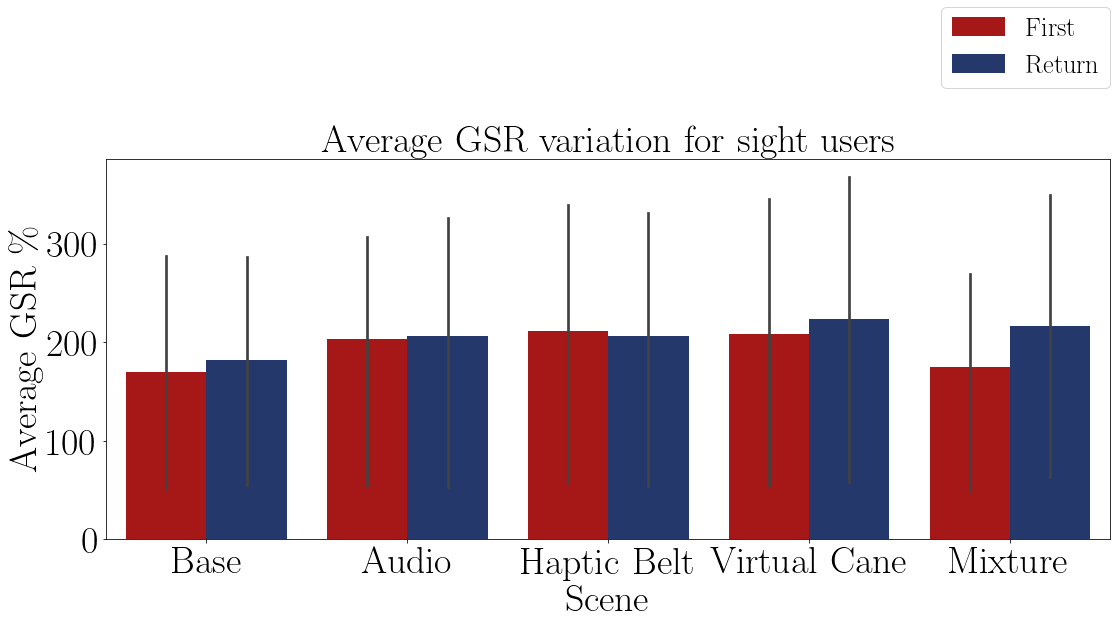
\includegraphics[width = 0.8\linewidth]{Resultados/GSR/Figuras/png/barplot_gsr_avg_scene_sight.png}
%        %\resizebox{0.6\linewidth}{!}{
%        %%% Creator: Matplotlib, PGF backend
%%
%% To include the figure in your LaTeX document, write
%%   \input{<filename>.pgf}
%%
%% Make sure the required packages are loaded in your preamble
%%   \usepackage{pgf}
%%
%% Figures using additional raster images can only be included by \input if
%% they are in the same directory as the main LaTeX file. For loading figures
%% from other directories you can use the `import` package
%%   \usepackage{import}
%%
%% and then include the figures with
%%   \import{<path to file>}{<filename>.pgf}
%%
%% Matplotlib used the following preamble
%%   \usepackage{fontspec}
%%
\begingroup%
\makeatletter%
\begin{pgfpicture}%
\pgfpathrectangle{\pgfpointorigin}{\pgfqpoint{15.281396in}{8.690562in}}%
\pgfusepath{use as bounding box, clip}%
\begin{pgfscope}%
\pgfsetbuttcap%
\pgfsetmiterjoin%
\pgfsetlinewidth{0.000000pt}%
\definecolor{currentstroke}{rgb}{1.000000,1.000000,1.000000}%
\pgfsetstrokecolor{currentstroke}%
\pgfsetstrokeopacity{0.000000}%
\pgfsetdash{}{0pt}%
\pgfpathmoveto{\pgfqpoint{0.000000in}{-0.000000in}}%
\pgfpathlineto{\pgfqpoint{15.281396in}{-0.000000in}}%
\pgfpathlineto{\pgfqpoint{15.281396in}{8.690562in}}%
\pgfpathlineto{\pgfqpoint{0.000000in}{8.690562in}}%
\pgfpathclose%
\pgfusepath{}%
\end{pgfscope}%
\begin{pgfscope}%
\pgfsetbuttcap%
\pgfsetmiterjoin%
\definecolor{currentfill}{rgb}{1.000000,1.000000,1.000000}%
\pgfsetfillcolor{currentfill}%
\pgfsetlinewidth{0.000000pt}%
\definecolor{currentstroke}{rgb}{0.000000,0.000000,0.000000}%
\pgfsetstrokecolor{currentstroke}%
\pgfsetstrokeopacity{0.000000}%
\pgfsetdash{}{0pt}%
\pgfpathmoveto{\pgfqpoint{1.231396in}{1.191562in}}%
\pgfpathlineto{\pgfqpoint{15.181396in}{1.191562in}}%
\pgfpathlineto{\pgfqpoint{15.181396in}{6.476562in}}%
\pgfpathlineto{\pgfqpoint{1.231396in}{6.476562in}}%
\pgfpathclose%
\pgfusepath{fill}%
\end{pgfscope}%
\begin{pgfscope}%
\pgfpathrectangle{\pgfqpoint{1.231396in}{1.191562in}}{\pgfqpoint{13.950000in}{5.285000in}}%
\pgfusepath{clip}%
\pgfsetbuttcap%
\pgfsetmiterjoin%
\definecolor{currentfill}{rgb}{0.651961,0.093137,0.093137}%
\pgfsetfillcolor{currentfill}%
\pgfsetlinewidth{0.000000pt}%
\definecolor{currentstroke}{rgb}{0.000000,0.000000,0.000000}%
\pgfsetstrokecolor{currentstroke}%
\pgfsetstrokeopacity{0.000000}%
\pgfsetdash{}{0pt}%
\pgfpathmoveto{\pgfqpoint{1.510396in}{1.191562in}}%
\pgfpathlineto{\pgfqpoint{2.626396in}{1.191562in}}%
\pgfpathlineto{\pgfqpoint{2.626396in}{3.511932in}}%
\pgfpathlineto{\pgfqpoint{1.510396in}{3.511932in}}%
\pgfpathclose%
\pgfusepath{fill}%
\end{pgfscope}%
\begin{pgfscope}%
\pgfpathrectangle{\pgfqpoint{1.231396in}{1.191562in}}{\pgfqpoint{13.950000in}{5.285000in}}%
\pgfusepath{clip}%
\pgfsetbuttcap%
\pgfsetmiterjoin%
\definecolor{currentfill}{rgb}{0.651961,0.093137,0.093137}%
\pgfsetfillcolor{currentfill}%
\pgfsetlinewidth{0.000000pt}%
\definecolor{currentstroke}{rgb}{0.000000,0.000000,0.000000}%
\pgfsetstrokecolor{currentstroke}%
\pgfsetstrokeopacity{0.000000}%
\pgfsetdash{}{0pt}%
\pgfpathmoveto{\pgfqpoint{4.300396in}{1.191562in}}%
\pgfpathlineto{\pgfqpoint{5.416396in}{1.191562in}}%
\pgfpathlineto{\pgfqpoint{5.416396in}{3.969940in}}%
\pgfpathlineto{\pgfqpoint{4.300396in}{3.969940in}}%
\pgfpathclose%
\pgfusepath{fill}%
\end{pgfscope}%
\begin{pgfscope}%
\pgfpathrectangle{\pgfqpoint{1.231396in}{1.191562in}}{\pgfqpoint{13.950000in}{5.285000in}}%
\pgfusepath{clip}%
\pgfsetbuttcap%
\pgfsetmiterjoin%
\definecolor{currentfill}{rgb}{0.651961,0.093137,0.093137}%
\pgfsetfillcolor{currentfill}%
\pgfsetlinewidth{0.000000pt}%
\definecolor{currentstroke}{rgb}{0.000000,0.000000,0.000000}%
\pgfsetstrokecolor{currentstroke}%
\pgfsetstrokeopacity{0.000000}%
\pgfsetdash{}{0pt}%
\pgfpathmoveto{\pgfqpoint{7.090396in}{1.191562in}}%
\pgfpathlineto{\pgfqpoint{8.206396in}{1.191562in}}%
\pgfpathlineto{\pgfqpoint{8.206396in}{4.086914in}}%
\pgfpathlineto{\pgfqpoint{7.090396in}{4.086914in}}%
\pgfpathclose%
\pgfusepath{fill}%
\end{pgfscope}%
\begin{pgfscope}%
\pgfpathrectangle{\pgfqpoint{1.231396in}{1.191562in}}{\pgfqpoint{13.950000in}{5.285000in}}%
\pgfusepath{clip}%
\pgfsetbuttcap%
\pgfsetmiterjoin%
\definecolor{currentfill}{rgb}{0.651961,0.093137,0.093137}%
\pgfsetfillcolor{currentfill}%
\pgfsetlinewidth{0.000000pt}%
\definecolor{currentstroke}{rgb}{0.000000,0.000000,0.000000}%
\pgfsetstrokecolor{currentstroke}%
\pgfsetstrokeopacity{0.000000}%
\pgfsetdash{}{0pt}%
\pgfpathmoveto{\pgfqpoint{9.880396in}{1.191562in}}%
\pgfpathlineto{\pgfqpoint{10.996396in}{1.191562in}}%
\pgfpathlineto{\pgfqpoint{10.996396in}{4.043061in}}%
\pgfpathlineto{\pgfqpoint{9.880396in}{4.043061in}}%
\pgfpathclose%
\pgfusepath{fill}%
\end{pgfscope}%
\begin{pgfscope}%
\pgfpathrectangle{\pgfqpoint{1.231396in}{1.191562in}}{\pgfqpoint{13.950000in}{5.285000in}}%
\pgfusepath{clip}%
\pgfsetbuttcap%
\pgfsetmiterjoin%
\definecolor{currentfill}{rgb}{0.651961,0.093137,0.093137}%
\pgfsetfillcolor{currentfill}%
\pgfsetlinewidth{0.000000pt}%
\definecolor{currentstroke}{rgb}{0.000000,0.000000,0.000000}%
\pgfsetstrokecolor{currentstroke}%
\pgfsetstrokeopacity{0.000000}%
\pgfsetdash{}{0pt}%
\pgfpathmoveto{\pgfqpoint{12.670396in}{1.191562in}}%
\pgfpathlineto{\pgfqpoint{13.786396in}{1.191562in}}%
\pgfpathlineto{\pgfqpoint{13.786396in}{3.591458in}}%
\pgfpathlineto{\pgfqpoint{12.670396in}{3.591458in}}%
\pgfpathclose%
\pgfusepath{fill}%
\end{pgfscope}%
\begin{pgfscope}%
\pgfpathrectangle{\pgfqpoint{1.231396in}{1.191562in}}{\pgfqpoint{13.950000in}{5.285000in}}%
\pgfusepath{clip}%
\pgfsetbuttcap%
\pgfsetmiterjoin%
\definecolor{currentfill}{rgb}{0.144608,0.218137,0.424020}%
\pgfsetfillcolor{currentfill}%
\pgfsetlinewidth{0.000000pt}%
\definecolor{currentstroke}{rgb}{0.000000,0.000000,0.000000}%
\pgfsetstrokecolor{currentstroke}%
\pgfsetstrokeopacity{0.000000}%
\pgfsetdash{}{0pt}%
\pgfpathmoveto{\pgfqpoint{2.626396in}{1.191562in}}%
\pgfpathlineto{\pgfqpoint{3.742396in}{1.191562in}}%
\pgfpathlineto{\pgfqpoint{3.742396in}{3.690373in}}%
\pgfpathlineto{\pgfqpoint{2.626396in}{3.690373in}}%
\pgfpathclose%
\pgfusepath{fill}%
\end{pgfscope}%
\begin{pgfscope}%
\pgfpathrectangle{\pgfqpoint{1.231396in}{1.191562in}}{\pgfqpoint{13.950000in}{5.285000in}}%
\pgfusepath{clip}%
\pgfsetbuttcap%
\pgfsetmiterjoin%
\definecolor{currentfill}{rgb}{0.144608,0.218137,0.424020}%
\pgfsetfillcolor{currentfill}%
\pgfsetlinewidth{0.000000pt}%
\definecolor{currentstroke}{rgb}{0.000000,0.000000,0.000000}%
\pgfsetstrokecolor{currentstroke}%
\pgfsetstrokeopacity{0.000000}%
\pgfsetdash{}{0pt}%
\pgfpathmoveto{\pgfqpoint{5.416396in}{1.191562in}}%
\pgfpathlineto{\pgfqpoint{6.532396in}{1.191562in}}%
\pgfpathlineto{\pgfqpoint{6.532396in}{4.013591in}}%
\pgfpathlineto{\pgfqpoint{5.416396in}{4.013591in}}%
\pgfpathclose%
\pgfusepath{fill}%
\end{pgfscope}%
\begin{pgfscope}%
\pgfpathrectangle{\pgfqpoint{1.231396in}{1.191562in}}{\pgfqpoint{13.950000in}{5.285000in}}%
\pgfusepath{clip}%
\pgfsetbuttcap%
\pgfsetmiterjoin%
\definecolor{currentfill}{rgb}{0.144608,0.218137,0.424020}%
\pgfsetfillcolor{currentfill}%
\pgfsetlinewidth{0.000000pt}%
\definecolor{currentstroke}{rgb}{0.000000,0.000000,0.000000}%
\pgfsetstrokecolor{currentstroke}%
\pgfsetstrokeopacity{0.000000}%
\pgfsetdash{}{0pt}%
\pgfpathmoveto{\pgfqpoint{8.206396in}{1.191562in}}%
\pgfpathlineto{\pgfqpoint{9.322396in}{1.191562in}}%
\pgfpathlineto{\pgfqpoint{9.322396in}{4.019938in}}%
\pgfpathlineto{\pgfqpoint{8.206396in}{4.019938in}}%
\pgfpathclose%
\pgfusepath{fill}%
\end{pgfscope}%
\begin{pgfscope}%
\pgfpathrectangle{\pgfqpoint{1.231396in}{1.191562in}}{\pgfqpoint{13.950000in}{5.285000in}}%
\pgfusepath{clip}%
\pgfsetbuttcap%
\pgfsetmiterjoin%
\definecolor{currentfill}{rgb}{0.144608,0.218137,0.424020}%
\pgfsetfillcolor{currentfill}%
\pgfsetlinewidth{0.000000pt}%
\definecolor{currentstroke}{rgb}{0.000000,0.000000,0.000000}%
\pgfsetstrokecolor{currentstroke}%
\pgfsetstrokeopacity{0.000000}%
\pgfsetdash{}{0pt}%
\pgfpathmoveto{\pgfqpoint{10.996396in}{1.191562in}}%
\pgfpathlineto{\pgfqpoint{12.112396in}{1.191562in}}%
\pgfpathlineto{\pgfqpoint{12.112396in}{4.247047in}}%
\pgfpathlineto{\pgfqpoint{10.996396in}{4.247047in}}%
\pgfpathclose%
\pgfusepath{fill}%
\end{pgfscope}%
\begin{pgfscope}%
\pgfpathrectangle{\pgfqpoint{1.231396in}{1.191562in}}{\pgfqpoint{13.950000in}{5.285000in}}%
\pgfusepath{clip}%
\pgfsetbuttcap%
\pgfsetmiterjoin%
\definecolor{currentfill}{rgb}{0.144608,0.218137,0.424020}%
\pgfsetfillcolor{currentfill}%
\pgfsetlinewidth{0.000000pt}%
\definecolor{currentstroke}{rgb}{0.000000,0.000000,0.000000}%
\pgfsetstrokecolor{currentstroke}%
\pgfsetstrokeopacity{0.000000}%
\pgfsetdash{}{0pt}%
\pgfpathmoveto{\pgfqpoint{13.786396in}{1.191562in}}%
\pgfpathlineto{\pgfqpoint{14.902396in}{1.191562in}}%
\pgfpathlineto{\pgfqpoint{14.902396in}{4.160726in}}%
\pgfpathlineto{\pgfqpoint{13.786396in}{4.160726in}}%
\pgfpathclose%
\pgfusepath{fill}%
\end{pgfscope}%
\begin{pgfscope}%
\pgfsetbuttcap%
\pgfsetroundjoin%
\definecolor{currentfill}{rgb}{0.000000,0.000000,0.000000}%
\pgfsetfillcolor{currentfill}%
\pgfsetlinewidth{0.803000pt}%
\definecolor{currentstroke}{rgb}{0.000000,0.000000,0.000000}%
\pgfsetstrokecolor{currentstroke}%
\pgfsetdash{}{0pt}%
\pgfsys@defobject{currentmarker}{\pgfqpoint{0.000000in}{-0.048611in}}{\pgfqpoint{0.000000in}{0.000000in}}{%
\pgfpathmoveto{\pgfqpoint{0.000000in}{0.000000in}}%
\pgfpathlineto{\pgfqpoint{0.000000in}{-0.048611in}}%
\pgfusepath{stroke,fill}%
}%
\begin{pgfscope}%
\pgfsys@transformshift{2.626396in}{1.191562in}%
\pgfsys@useobject{currentmarker}{}%
\end{pgfscope}%
\end{pgfscope}%
\begin{pgfscope}%
\definecolor{textcolor}{rgb}{0.000000,0.000000,0.000000}%
\pgfsetstrokecolor{textcolor}%
\pgfsetfillcolor{textcolor}%
\pgftext[x=2.626396in,y=1.094339in,,top]{\color{textcolor}\rmfamily\fontsize{38.016000}{45.619200}\selectfont Base}%
\end{pgfscope}%
\begin{pgfscope}%
\pgfsetbuttcap%
\pgfsetroundjoin%
\definecolor{currentfill}{rgb}{0.000000,0.000000,0.000000}%
\pgfsetfillcolor{currentfill}%
\pgfsetlinewidth{0.803000pt}%
\definecolor{currentstroke}{rgb}{0.000000,0.000000,0.000000}%
\pgfsetstrokecolor{currentstroke}%
\pgfsetdash{}{0pt}%
\pgfsys@defobject{currentmarker}{\pgfqpoint{0.000000in}{-0.048611in}}{\pgfqpoint{0.000000in}{0.000000in}}{%
\pgfpathmoveto{\pgfqpoint{0.000000in}{0.000000in}}%
\pgfpathlineto{\pgfqpoint{0.000000in}{-0.048611in}}%
\pgfusepath{stroke,fill}%
}%
\begin{pgfscope}%
\pgfsys@transformshift{5.416396in}{1.191562in}%
\pgfsys@useobject{currentmarker}{}%
\end{pgfscope}%
\end{pgfscope}%
\begin{pgfscope}%
\definecolor{textcolor}{rgb}{0.000000,0.000000,0.000000}%
\pgfsetstrokecolor{textcolor}%
\pgfsetfillcolor{textcolor}%
\pgftext[x=5.416396in,y=1.094339in,,top]{\color{textcolor}\rmfamily\fontsize{38.016000}{45.619200}\selectfont Audio}%
\end{pgfscope}%
\begin{pgfscope}%
\pgfsetbuttcap%
\pgfsetroundjoin%
\definecolor{currentfill}{rgb}{0.000000,0.000000,0.000000}%
\pgfsetfillcolor{currentfill}%
\pgfsetlinewidth{0.803000pt}%
\definecolor{currentstroke}{rgb}{0.000000,0.000000,0.000000}%
\pgfsetstrokecolor{currentstroke}%
\pgfsetdash{}{0pt}%
\pgfsys@defobject{currentmarker}{\pgfqpoint{0.000000in}{-0.048611in}}{\pgfqpoint{0.000000in}{0.000000in}}{%
\pgfpathmoveto{\pgfqpoint{0.000000in}{0.000000in}}%
\pgfpathlineto{\pgfqpoint{0.000000in}{-0.048611in}}%
\pgfusepath{stroke,fill}%
}%
\begin{pgfscope}%
\pgfsys@transformshift{8.206396in}{1.191562in}%
\pgfsys@useobject{currentmarker}{}%
\end{pgfscope}%
\end{pgfscope}%
\begin{pgfscope}%
\definecolor{textcolor}{rgb}{0.000000,0.000000,0.000000}%
\pgfsetstrokecolor{textcolor}%
\pgfsetfillcolor{textcolor}%
\pgftext[x=8.206396in,y=1.094339in,,top]{\color{textcolor}\rmfamily\fontsize{38.016000}{45.619200}\selectfont Haptic Belt}%
\end{pgfscope}%
\begin{pgfscope}%
\pgfsetbuttcap%
\pgfsetroundjoin%
\definecolor{currentfill}{rgb}{0.000000,0.000000,0.000000}%
\pgfsetfillcolor{currentfill}%
\pgfsetlinewidth{0.803000pt}%
\definecolor{currentstroke}{rgb}{0.000000,0.000000,0.000000}%
\pgfsetstrokecolor{currentstroke}%
\pgfsetdash{}{0pt}%
\pgfsys@defobject{currentmarker}{\pgfqpoint{0.000000in}{-0.048611in}}{\pgfqpoint{0.000000in}{0.000000in}}{%
\pgfpathmoveto{\pgfqpoint{0.000000in}{0.000000in}}%
\pgfpathlineto{\pgfqpoint{0.000000in}{-0.048611in}}%
\pgfusepath{stroke,fill}%
}%
\begin{pgfscope}%
\pgfsys@transformshift{10.996396in}{1.191562in}%
\pgfsys@useobject{currentmarker}{}%
\end{pgfscope}%
\end{pgfscope}%
\begin{pgfscope}%
\definecolor{textcolor}{rgb}{0.000000,0.000000,0.000000}%
\pgfsetstrokecolor{textcolor}%
\pgfsetfillcolor{textcolor}%
\pgftext[x=10.996396in,y=1.094339in,,top]{\color{textcolor}\rmfamily\fontsize{38.016000}{45.619200}\selectfont Virtual Cane}%
\end{pgfscope}%
\begin{pgfscope}%
\pgfsetbuttcap%
\pgfsetroundjoin%
\definecolor{currentfill}{rgb}{0.000000,0.000000,0.000000}%
\pgfsetfillcolor{currentfill}%
\pgfsetlinewidth{0.803000pt}%
\definecolor{currentstroke}{rgb}{0.000000,0.000000,0.000000}%
\pgfsetstrokecolor{currentstroke}%
\pgfsetdash{}{0pt}%
\pgfsys@defobject{currentmarker}{\pgfqpoint{0.000000in}{-0.048611in}}{\pgfqpoint{0.000000in}{0.000000in}}{%
\pgfpathmoveto{\pgfqpoint{0.000000in}{0.000000in}}%
\pgfpathlineto{\pgfqpoint{0.000000in}{-0.048611in}}%
\pgfusepath{stroke,fill}%
}%
\begin{pgfscope}%
\pgfsys@transformshift{13.786396in}{1.191562in}%
\pgfsys@useobject{currentmarker}{}%
\end{pgfscope}%
\end{pgfscope}%
\begin{pgfscope}%
\definecolor{textcolor}{rgb}{0.000000,0.000000,0.000000}%
\pgfsetstrokecolor{textcolor}%
\pgfsetfillcolor{textcolor}%
\pgftext[x=13.786396in,y=1.094339in,,top]{\color{textcolor}\rmfamily\fontsize{38.016000}{45.619200}\selectfont Mixture}%
\end{pgfscope}%
\begin{pgfscope}%
\definecolor{textcolor}{rgb}{0.000000,0.000000,0.000000}%
\pgfsetstrokecolor{textcolor}%
\pgfsetfillcolor{textcolor}%
\pgftext[x=8.206396in,y=0.569392in,,top]{\color{textcolor}\rmfamily\fontsize{38.016000}{45.619200}\selectfont Scene}%
\end{pgfscope}%
\begin{pgfscope}%
\pgfsetbuttcap%
\pgfsetroundjoin%
\definecolor{currentfill}{rgb}{0.000000,0.000000,0.000000}%
\pgfsetfillcolor{currentfill}%
\pgfsetlinewidth{0.803000pt}%
\definecolor{currentstroke}{rgb}{0.000000,0.000000,0.000000}%
\pgfsetstrokecolor{currentstroke}%
\pgfsetdash{}{0pt}%
\pgfsys@defobject{currentmarker}{\pgfqpoint{-0.048611in}{0.000000in}}{\pgfqpoint{-0.000000in}{0.000000in}}{%
\pgfpathmoveto{\pgfqpoint{-0.000000in}{0.000000in}}%
\pgfpathlineto{\pgfqpoint{-0.048611in}{0.000000in}}%
\pgfusepath{stroke,fill}%
}%
\begin{pgfscope}%
\pgfsys@transformshift{1.231396in}{1.191562in}%
\pgfsys@useobject{currentmarker}{}%
\end{pgfscope}%
\end{pgfscope}%
\begin{pgfscope}%
\definecolor{textcolor}{rgb}{0.000000,0.000000,0.000000}%
\pgfsetstrokecolor{textcolor}%
\pgfsetfillcolor{textcolor}%
\pgftext[x=0.975695in, y=1.008346in, left, base]{\color{textcolor}\rmfamily\fontsize{38.016000}{45.619200}\selectfont \(\displaystyle {0}\)}%
\end{pgfscope}%
\begin{pgfscope}%
\pgfsetbuttcap%
\pgfsetroundjoin%
\definecolor{currentfill}{rgb}{0.000000,0.000000,0.000000}%
\pgfsetfillcolor{currentfill}%
\pgfsetlinewidth{0.803000pt}%
\definecolor{currentstroke}{rgb}{0.000000,0.000000,0.000000}%
\pgfsetstrokecolor{currentstroke}%
\pgfsetdash{}{0pt}%
\pgfsys@defobject{currentmarker}{\pgfqpoint{-0.048611in}{0.000000in}}{\pgfqpoint{-0.000000in}{0.000000in}}{%
\pgfpathmoveto{\pgfqpoint{-0.000000in}{0.000000in}}%
\pgfpathlineto{\pgfqpoint{-0.048611in}{0.000000in}}%
\pgfusepath{stroke,fill}%
}%
\begin{pgfscope}%
\pgfsys@transformshift{1.231396in}{2.560159in}%
\pgfsys@useobject{currentmarker}{}%
\end{pgfscope}%
\end{pgfscope}%
\begin{pgfscope}%
\definecolor{textcolor}{rgb}{0.000000,0.000000,0.000000}%
\pgfsetstrokecolor{textcolor}%
\pgfsetfillcolor{textcolor}%
\pgftext[x=0.658739in, y=2.376942in, left, base]{\color{textcolor}\rmfamily\fontsize{38.016000}{45.619200}\selectfont \(\displaystyle {100}\)}%
\end{pgfscope}%
\begin{pgfscope}%
\pgfsetbuttcap%
\pgfsetroundjoin%
\definecolor{currentfill}{rgb}{0.000000,0.000000,0.000000}%
\pgfsetfillcolor{currentfill}%
\pgfsetlinewidth{0.803000pt}%
\definecolor{currentstroke}{rgb}{0.000000,0.000000,0.000000}%
\pgfsetstrokecolor{currentstroke}%
\pgfsetdash{}{0pt}%
\pgfsys@defobject{currentmarker}{\pgfqpoint{-0.048611in}{0.000000in}}{\pgfqpoint{-0.000000in}{0.000000in}}{%
\pgfpathmoveto{\pgfqpoint{-0.000000in}{0.000000in}}%
\pgfpathlineto{\pgfqpoint{-0.048611in}{0.000000in}}%
\pgfusepath{stroke,fill}%
}%
\begin{pgfscope}%
\pgfsys@transformshift{1.231396in}{3.928755in}%
\pgfsys@useobject{currentmarker}{}%
\end{pgfscope}%
\end{pgfscope}%
\begin{pgfscope}%
\definecolor{textcolor}{rgb}{0.000000,0.000000,0.000000}%
\pgfsetstrokecolor{textcolor}%
\pgfsetfillcolor{textcolor}%
\pgftext[x=0.658739in, y=3.745539in, left, base]{\color{textcolor}\rmfamily\fontsize{38.016000}{45.619200}\selectfont \(\displaystyle {200}\)}%
\end{pgfscope}%
\begin{pgfscope}%
\pgfsetbuttcap%
\pgfsetroundjoin%
\definecolor{currentfill}{rgb}{0.000000,0.000000,0.000000}%
\pgfsetfillcolor{currentfill}%
\pgfsetlinewidth{0.803000pt}%
\definecolor{currentstroke}{rgb}{0.000000,0.000000,0.000000}%
\pgfsetstrokecolor{currentstroke}%
\pgfsetdash{}{0pt}%
\pgfsys@defobject{currentmarker}{\pgfqpoint{-0.048611in}{0.000000in}}{\pgfqpoint{-0.000000in}{0.000000in}}{%
\pgfpathmoveto{\pgfqpoint{-0.000000in}{0.000000in}}%
\pgfpathlineto{\pgfqpoint{-0.048611in}{0.000000in}}%
\pgfusepath{stroke,fill}%
}%
\begin{pgfscope}%
\pgfsys@transformshift{1.231396in}{5.297352in}%
\pgfsys@useobject{currentmarker}{}%
\end{pgfscope}%
\end{pgfscope}%
\begin{pgfscope}%
\definecolor{textcolor}{rgb}{0.000000,0.000000,0.000000}%
\pgfsetstrokecolor{textcolor}%
\pgfsetfillcolor{textcolor}%
\pgftext[x=0.658739in, y=5.114136in, left, base]{\color{textcolor}\rmfamily\fontsize{38.016000}{45.619200}\selectfont \(\displaystyle {300}\)}%
\end{pgfscope}%
\begin{pgfscope}%
\definecolor{textcolor}{rgb}{0.000000,0.000000,0.000000}%
\pgfsetstrokecolor{textcolor}%
\pgfsetfillcolor{textcolor}%
\pgftext[x=0.603184in,y=3.834062in,,bottom,rotate=90.000000]{\color{textcolor}\rmfamily\fontsize{38.016000}{45.619200}\selectfont Average GSR \%}%
\end{pgfscope}%
\begin{pgfscope}%
\pgfpathrectangle{\pgfqpoint{1.231396in}{1.191562in}}{\pgfqpoint{13.950000in}{5.285000in}}%
\pgfusepath{clip}%
\pgfsetrectcap%
\pgfsetroundjoin%
\pgfsetlinewidth{2.710125pt}%
\definecolor{currentstroke}{rgb}{0.260000,0.260000,0.260000}%
\pgfsetstrokecolor{currentstroke}%
\pgfsetdash{}{0pt}%
\pgfpathmoveto{\pgfqpoint{2.068396in}{1.897169in}}%
\pgfpathlineto{\pgfqpoint{2.068396in}{5.126695in}}%
\pgfusepath{stroke}%
\end{pgfscope}%
\begin{pgfscope}%
\pgfpathrectangle{\pgfqpoint{1.231396in}{1.191562in}}{\pgfqpoint{13.950000in}{5.285000in}}%
\pgfusepath{clip}%
\pgfsetrectcap%
\pgfsetroundjoin%
\pgfsetlinewidth{2.710125pt}%
\definecolor{currentstroke}{rgb}{0.260000,0.260000,0.260000}%
\pgfsetstrokecolor{currentstroke}%
\pgfsetdash{}{0pt}%
\pgfpathmoveto{\pgfqpoint{4.858396in}{1.943825in}}%
\pgfpathlineto{\pgfqpoint{4.858396in}{5.444463in}}%
\pgfusepath{stroke}%
\end{pgfscope}%
\begin{pgfscope}%
\pgfpathrectangle{\pgfqpoint{1.231396in}{1.191562in}}{\pgfqpoint{13.950000in}{5.285000in}}%
\pgfusepath{clip}%
\pgfsetrectcap%
\pgfsetroundjoin%
\pgfsetlinewidth{2.710125pt}%
\definecolor{currentstroke}{rgb}{0.260000,0.260000,0.260000}%
\pgfsetstrokecolor{currentstroke}%
\pgfsetdash{}{0pt}%
\pgfpathmoveto{\pgfqpoint{7.648396in}{1.981923in}}%
\pgfpathlineto{\pgfqpoint{7.648396in}{5.839132in}}%
\pgfusepath{stroke}%
\end{pgfscope}%
\begin{pgfscope}%
\pgfpathrectangle{\pgfqpoint{1.231396in}{1.191562in}}{\pgfqpoint{13.950000in}{5.285000in}}%
\pgfusepath{clip}%
\pgfsetrectcap%
\pgfsetroundjoin%
\pgfsetlinewidth{2.710125pt}%
\definecolor{currentstroke}{rgb}{0.260000,0.260000,0.260000}%
\pgfsetstrokecolor{currentstroke}%
\pgfsetdash{}{0pt}%
\pgfpathmoveto{\pgfqpoint{10.438396in}{1.938265in}}%
\pgfpathlineto{\pgfqpoint{10.438396in}{5.917850in}}%
\pgfusepath{stroke}%
\end{pgfscope}%
\begin{pgfscope}%
\pgfpathrectangle{\pgfqpoint{1.231396in}{1.191562in}}{\pgfqpoint{13.950000in}{5.285000in}}%
\pgfusepath{clip}%
\pgfsetrectcap%
\pgfsetroundjoin%
\pgfsetlinewidth{2.710125pt}%
\definecolor{currentstroke}{rgb}{0.260000,0.260000,0.260000}%
\pgfsetstrokecolor{currentstroke}%
\pgfsetdash{}{0pt}%
\pgfpathmoveto{\pgfqpoint{13.228396in}{1.861914in}}%
\pgfpathlineto{\pgfqpoint{13.228396in}{4.872615in}}%
\pgfusepath{stroke}%
\end{pgfscope}%
\begin{pgfscope}%
\pgfpathrectangle{\pgfqpoint{1.231396in}{1.191562in}}{\pgfqpoint{13.950000in}{5.285000in}}%
\pgfusepath{clip}%
\pgfsetrectcap%
\pgfsetroundjoin%
\pgfsetlinewidth{2.710125pt}%
\definecolor{currentstroke}{rgb}{0.260000,0.260000,0.260000}%
\pgfsetstrokecolor{currentstroke}%
\pgfsetdash{}{0pt}%
\pgfpathmoveto{\pgfqpoint{3.184396in}{1.941799in}}%
\pgfpathlineto{\pgfqpoint{3.184396in}{5.115308in}}%
\pgfusepath{stroke}%
\end{pgfscope}%
\begin{pgfscope}%
\pgfpathrectangle{\pgfqpoint{1.231396in}{1.191562in}}{\pgfqpoint{13.950000in}{5.285000in}}%
\pgfusepath{clip}%
\pgfsetrectcap%
\pgfsetroundjoin%
\pgfsetlinewidth{2.710125pt}%
\definecolor{currentstroke}{rgb}{0.260000,0.260000,0.260000}%
\pgfsetstrokecolor{currentstroke}%
\pgfsetdash{}{0pt}%
\pgfpathmoveto{\pgfqpoint{5.974396in}{1.924633in}}%
\pgfpathlineto{\pgfqpoint{5.974396in}{5.658833in}}%
\pgfusepath{stroke}%
\end{pgfscope}%
\begin{pgfscope}%
\pgfpathrectangle{\pgfqpoint{1.231396in}{1.191562in}}{\pgfqpoint{13.950000in}{5.285000in}}%
\pgfusepath{clip}%
\pgfsetrectcap%
\pgfsetroundjoin%
\pgfsetlinewidth{2.710125pt}%
\definecolor{currentstroke}{rgb}{0.260000,0.260000,0.260000}%
\pgfsetstrokecolor{currentstroke}%
\pgfsetdash{}{0pt}%
\pgfpathmoveto{\pgfqpoint{8.764396in}{1.935764in}}%
\pgfpathlineto{\pgfqpoint{8.764396in}{5.859791in}}%
\pgfusepath{stroke}%
\end{pgfscope}%
\begin{pgfscope}%
\pgfpathrectangle{\pgfqpoint{1.231396in}{1.191562in}}{\pgfqpoint{13.950000in}{5.285000in}}%
\pgfusepath{clip}%
\pgfsetrectcap%
\pgfsetroundjoin%
\pgfsetlinewidth{2.710125pt}%
\definecolor{currentstroke}{rgb}{0.260000,0.260000,0.260000}%
\pgfsetstrokecolor{currentstroke}%
\pgfsetdash{}{0pt}%
\pgfpathmoveto{\pgfqpoint{11.554396in}{1.819956in}}%
\pgfpathlineto{\pgfqpoint{11.554396in}{6.224895in}}%
\pgfusepath{stroke}%
\end{pgfscope}%
\begin{pgfscope}%
\pgfpathrectangle{\pgfqpoint{1.231396in}{1.191562in}}{\pgfqpoint{13.950000in}{5.285000in}}%
\pgfusepath{clip}%
\pgfsetrectcap%
\pgfsetroundjoin%
\pgfsetlinewidth{2.710125pt}%
\definecolor{currentstroke}{rgb}{0.260000,0.260000,0.260000}%
\pgfsetstrokecolor{currentstroke}%
\pgfsetdash{}{0pt}%
\pgfpathmoveto{\pgfqpoint{14.344396in}{2.061192in}}%
\pgfpathlineto{\pgfqpoint{14.344396in}{5.973347in}}%
\pgfusepath{stroke}%
\end{pgfscope}%
\begin{pgfscope}%
\pgfsetrectcap%
\pgfsetmiterjoin%
\pgfsetlinewidth{0.803000pt}%
\definecolor{currentstroke}{rgb}{0.000000,0.000000,0.000000}%
\pgfsetstrokecolor{currentstroke}%
\pgfsetdash{}{0pt}%
\pgfpathmoveto{\pgfqpoint{1.231396in}{1.191562in}}%
\pgfpathlineto{\pgfqpoint{1.231396in}{6.476562in}}%
\pgfusepath{stroke}%
\end{pgfscope}%
\begin{pgfscope}%
\pgfsetrectcap%
\pgfsetmiterjoin%
\pgfsetlinewidth{0.803000pt}%
\definecolor{currentstroke}{rgb}{0.000000,0.000000,0.000000}%
\pgfsetstrokecolor{currentstroke}%
\pgfsetdash{}{0pt}%
\pgfpathmoveto{\pgfqpoint{15.181396in}{1.191562in}}%
\pgfpathlineto{\pgfqpoint{15.181396in}{6.476562in}}%
\pgfusepath{stroke}%
\end{pgfscope}%
\begin{pgfscope}%
\pgfsetrectcap%
\pgfsetmiterjoin%
\pgfsetlinewidth{0.803000pt}%
\definecolor{currentstroke}{rgb}{0.000000,0.000000,0.000000}%
\pgfsetstrokecolor{currentstroke}%
\pgfsetdash{}{0pt}%
\pgfpathmoveto{\pgfqpoint{1.231396in}{1.191562in}}%
\pgfpathlineto{\pgfqpoint{15.181396in}{1.191562in}}%
\pgfusepath{stroke}%
\end{pgfscope}%
\begin{pgfscope}%
\pgfsetrectcap%
\pgfsetmiterjoin%
\pgfsetlinewidth{0.803000pt}%
\definecolor{currentstroke}{rgb}{0.000000,0.000000,0.000000}%
\pgfsetstrokecolor{currentstroke}%
\pgfsetdash{}{0pt}%
\pgfpathmoveto{\pgfqpoint{1.231396in}{6.476562in}}%
\pgfpathlineto{\pgfqpoint{15.181396in}{6.476562in}}%
\pgfusepath{stroke}%
\end{pgfscope}%
\begin{pgfscope}%
\definecolor{textcolor}{rgb}{0.000000,0.000000,0.000000}%
\pgfsetstrokecolor{textcolor}%
\pgfsetfillcolor{textcolor}%
\pgftext[x=8.206396in,y=6.584273in,,base]{\color{textcolor}\rmfamily\fontsize{38.016000}{45.619200}\selectfont Average GSR variation for sight users}%
\end{pgfscope}%
\begin{pgfscope}%
\pgfsetbuttcap%
\pgfsetmiterjoin%
\definecolor{currentfill}{rgb}{1.000000,1.000000,1.000000}%
\pgfsetfillcolor{currentfill}%
\pgfsetfillopacity{0.800000}%
\pgfsetlinewidth{1.003750pt}%
\definecolor{currentstroke}{rgb}{0.800000,0.800000,0.800000}%
\pgfsetstrokecolor{currentstroke}%
\pgfsetstrokeopacity{0.800000}%
\pgfsetdash{}{0pt}%
\pgfpathmoveto{\pgfqpoint{12.902196in}{7.457562in}}%
\pgfpathlineto{\pgfqpoint{15.108062in}{7.457562in}}%
\pgfpathquadraticcurveto{\pgfqpoint{15.181396in}{7.457562in}}{\pgfqpoint{15.181396in}{7.530896in}}%
\pgfpathlineto{\pgfqpoint{15.181396in}{8.517228in}}%
\pgfpathquadraticcurveto{\pgfqpoint{15.181396in}{8.590562in}}{\pgfqpoint{15.108062in}{8.590562in}}%
\pgfpathlineto{\pgfqpoint{12.902196in}{8.590562in}}%
\pgfpathquadraticcurveto{\pgfqpoint{12.828862in}{8.590562in}}{\pgfqpoint{12.828862in}{8.517228in}}%
\pgfpathlineto{\pgfqpoint{12.828862in}{7.530896in}}%
\pgfpathquadraticcurveto{\pgfqpoint{12.828862in}{7.457562in}}{\pgfqpoint{12.902196in}{7.457562in}}%
\pgfpathclose%
\pgfusepath{stroke,fill}%
\end{pgfscope}%
\begin{pgfscope}%
\pgfsetbuttcap%
\pgfsetmiterjoin%
\definecolor{currentfill}{rgb}{0.651961,0.093137,0.093137}%
\pgfsetfillcolor{currentfill}%
\pgfsetlinewidth{0.000000pt}%
\definecolor{currentstroke}{rgb}{0.000000,0.000000,0.000000}%
\pgfsetstrokecolor{currentstroke}%
\pgfsetstrokeopacity{0.000000}%
\pgfsetdash{}{0pt}%
\pgfpathmoveto{\pgfqpoint{12.975529in}{8.187228in}}%
\pgfpathlineto{\pgfqpoint{13.708862in}{8.187228in}}%
\pgfpathlineto{\pgfqpoint{13.708862in}{8.443895in}}%
\pgfpathlineto{\pgfqpoint{12.975529in}{8.443895in}}%
\pgfpathclose%
\pgfusepath{fill}%
\end{pgfscope}%
\begin{pgfscope}%
\definecolor{textcolor}{rgb}{0.000000,0.000000,0.000000}%
\pgfsetstrokecolor{textcolor}%
\pgfsetfillcolor{textcolor}%
\pgftext[x=14.002196in,y=8.187228in,left,base]{\color{textcolor}\rmfamily\fontsize{26.400000}{31.680000}\selectfont First}%
\end{pgfscope}%
\begin{pgfscope}%
\pgfsetbuttcap%
\pgfsetmiterjoin%
\definecolor{currentfill}{rgb}{0.144608,0.218137,0.424020}%
\pgfsetfillcolor{currentfill}%
\pgfsetlinewidth{0.000000pt}%
\definecolor{currentstroke}{rgb}{0.000000,0.000000,0.000000}%
\pgfsetstrokecolor{currentstroke}%
\pgfsetstrokeopacity{0.000000}%
\pgfsetdash{}{0pt}%
\pgfpathmoveto{\pgfqpoint{12.975529in}{7.675729in}}%
\pgfpathlineto{\pgfqpoint{13.708862in}{7.675729in}}%
\pgfpathlineto{\pgfqpoint{13.708862in}{7.932395in}}%
\pgfpathlineto{\pgfqpoint{12.975529in}{7.932395in}}%
\pgfpathclose%
\pgfusepath{fill}%
\end{pgfscope}%
\begin{pgfscope}%
\definecolor{textcolor}{rgb}{0.000000,0.000000,0.000000}%
\pgfsetstrokecolor{textcolor}%
\pgfsetfillcolor{textcolor}%
\pgftext[x=14.002196in,y=7.675729in,left,base]{\color{textcolor}\rmfamily\fontsize{26.400000}{31.680000}\selectfont Return}%
\end{pgfscope}%
\end{pgfpicture}%
\makeatother%
\endgroup%
    
%        %}
%        \caption{Bar plot of the average skin conductance of the sighted participants on each method.}
%        \label{fig:barplot_gsr_scene_sight}
%    \end{minipage}
%\end{figure}

The Figure \ref{fig:boxplot_ecg_bpm_scene} shows a comparison between both groups

%\begin{figure}[!htb]
%    %\centering
%    \begin{minipage}{.45\linewidth}
%        \centering
%        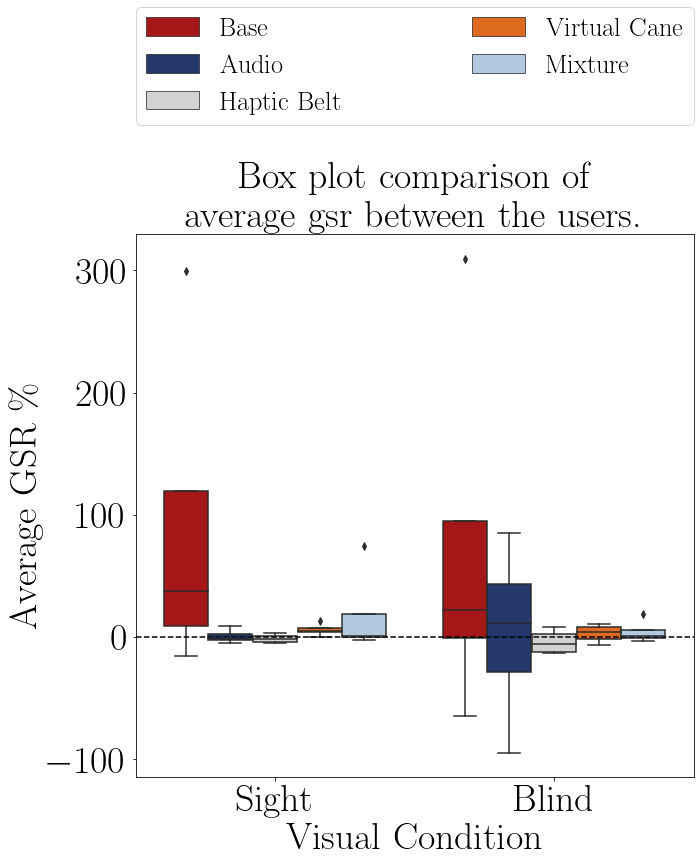
\includegraphics[width = \linewidth]{Resultados/GSR/Figuras/png/boxplot_gsr_avg_scene.png}
%        \caption{Boxplot of the average skin conductace of the participants on each method.}
%        \label{fig:boxplot_gsr_scene}
%    \end{minipage}
%    \begin{minipage}{.1\linewidth}
%        \hfill
%    \end{minipage}
%    \begin{minipage}{.45\linewidth}
%        \vspace{1.8cm}
%        \centering
%        %\hspace{-4cm}
%        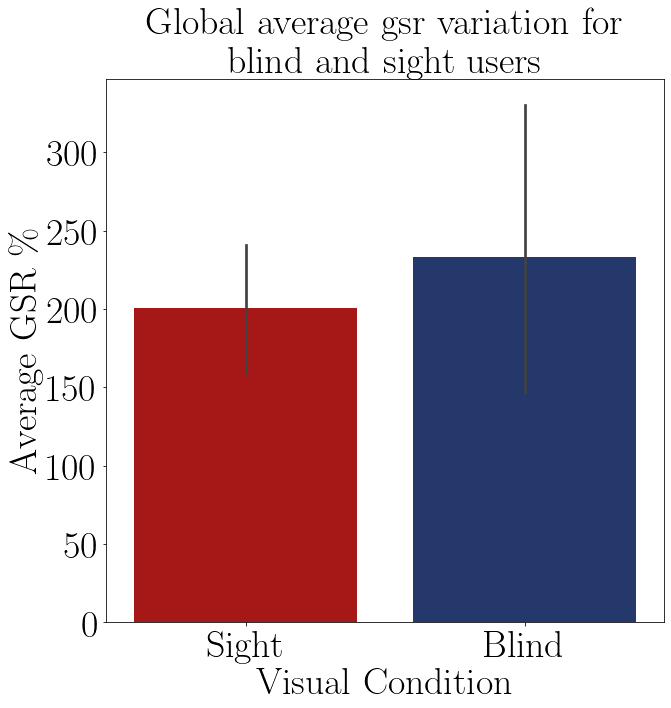
\includegraphics[width = \linewidth]{Resultados/GSR/Figuras/png/barplot_gsr_avg.png}
%        \caption{Bar plot of the average GSR of of each group.}
%        \label{fig:barplot_gsr_avg}
%    \end{minipage}
%\end{figure}

The Table \ref{tab:gsr_avg_table_def2} shows the variation of the heartbeat in each round of each group. It is also possible to notice the same increase noticed before.

%
\begin{table}[!htb]
\centering
\caption{Average GSR variation in relation to the baseline grouped by participant and visual Condition.}
\label{tab:gsr_avg_table_def2}
\begin{tabular}{lllrrrrrr}
\toprule
{} &     Base &    Audio & \begin{tabular}[c]{@{}l@{}}Haptic\\ Belt\end{tabular} & \begin{tabular}[c]{@{}l@{}}Virtual\\ Cane\end{tabular} &  Mixture \\
Visual Condition &          &          &                                                       &                                                        &          \\
\midrule
Blind            &  141.1\% &  127.3\% &                                               244.6\% &                                                307.2\% &  344.4\% \\
Sight            &  176.1\% &  204.6\% &                                               209.1\% &                                                215.8\% &  196.2\% \\
\bottomrule
\end{tabular}
\end{table}



The Shapiro–Wilk normality test on the Table \ref{tab:shapiro_gsr_avg} shows that only the "Audio" method is normally distributed for the "blind" sample while for the "sight" sample only the "Virtual Cane" is not normally distributed

According to the T-Test presented in the Table \ref{tab:ttest_gsr} there is no difference in the skin conductace  frequency variation between the sample groups.


%\begin{table}[!htb]
%    \begin{minipage}{.45\linewidth}
%        
\centering
\caption{Shapiro test p-value for the gsr average for each method and visual condition}
\label{tab:shapiro_gsr_avg}
\begin{tabular}{lr}
\toprule
            Method &  Shapiro P-Value \\
\midrule
        Base blind &            0.002 \\
        Base sight &            0.187 \\
       Audio blind &            0.544 \\
       Audio sight &            0.046 \\
 Haptic Belt blind &            0.017 \\
 Haptic Belt sight &            0.155 \\
Virtual Cane blind &            0.004 \\
Virtual Cane sight &            0.275 \\
     Mixture blind &            0.011 \\
     Mixture sight &            0.376 \\
\bottomrule
\end{tabular}

%    \end{minipage}
%    \hfill
%    \begin{minipage}{.45\linewidth}
%        \vspace{-2.75cm}
%        
\centering
\begin{tabular}{lr}
\toprule
      Method & T-Test P-Value \\
\midrule
        Base &        0.002** \\
       Audio &        0.022** \\
 Haptic Belt &          0.728 \\
Virtual Cane &          0.523 \\
     Mixture &          0.336 \\
\bottomrule
\end{tabular}

%    \end{minipage}
%\end{table}

The Table \ref{tab:repblocanova_gsr} shows the Anova test p-value of the skin conductance frequency of the "blind" sample between the guidance methods presented in the Table \ref{tab:gsr_avg_table}. The p-value indicates that there is at least one method that is statistically equal to one of the other methods.

%
\begin{table}[!htb]
\centering
\caption{Anova p-value for the GSR score on each method for blinded users.}
\label{tab:blocanova_gsr_avg}
\begin{tabular}{lrrrrr}
\toprule
               Source &  Squared sum &  DOF & Squared average &     F & \begin{tabular}[c]{@{}l@{}}P-Value \\ $(F_{0} > F)$\end{tabular} \\
\midrule
Participants (blocks) &  1918983.649 &    3 &      221654.067 & 9.552 &                                                                  \\
               Method &   886616.269 &    4 &      639661.216 & 3.310 &                                                          0.048** \\
   Experimental error &   803557.557 &   12 &       66963.130 &       &                                                                  \\
                Total &  3609157.475 &   39 &                 &       &                                                                  \\
\bottomrule
\end{tabular}
\end{table}



The Table \ref{tab:lsd_gsr} presents the conclusion of a pairwise Fisher LSD test of the blind skin conductance frequency variation between all the guidance methods. The results show that the "Virtual Cane" and the "Mixture" have different variations, but since they are not normally distributed this conclusion can not statistically be made.

%
\begin{table}[!htb]
\centering
\caption{Cross validation p-value for the GSR on each method for blinded users.}
\label{tab:lsd_gsr_avg}
\begin{tabular}{rclr}
\toprule
      \multicolumn{3}{c}{Method} &                                       Analysis \\
\midrule
              Base & $X$ & Audio &               $H_0 : \mu_{Base} = \mu_{Audio}$ \\
        Base & $X$ & Haptic Belt &         $H_0 : \mu_{Base} = \mu_{Haptic Belt}$ \\
       Base & $X$ & Virtual Cane &    $H_1 : \mu_{Base} \ne \mu_{Virtual Cane}**$ \\
            Base & $X$ & Mixture &         $H_1 : \mu_{Base} \ne \mu_{Mixture}**$ \\
       Audio & $X$ & Haptic Belt &    $H_1 : \mu_{Audio} \ne \mu_{Haptic Belt}**$ \\
      Audio & $X$ & Virtual Cane &   $H_1 : \mu_{Audio} \ne \mu_{Virtual Cane}**$ \\
           Audio & $X$ & Mixture &        $H_1 : \mu_{Audio} \ne \mu_{Mixture}**$ \\
Haptic Belt & $X$ & Virtual Cane & $H_0 : \mu_{Haptic Belt} = \mu_{Virtual Cane}$ \\
     Haptic Belt & $X$ & Mixture &      $H_0 : \mu_{Haptic Belt} = \mu_{Mixture}$ \\
    Virtual Cane & $X$ & Mixture &     $H_0 : \mu_{Virtual Cane} = \mu_{Mixture}$ \\
\bottomrule
\end{tabular}
\end{table}



According to the Anova test at Table \ref{tab:repblocanova_gsr} and the LSD test at \ref{tab:lsd_gsr} only the "Virtual Cane" and the "Mixture" method provoked a different reaction than the "Base" method, but since the Shapiro test at the Table \ref{tab:shapiro_gsr_avg} showed that they are not normally distributed, than this conclusion has no foundation.

\subsubsection{Analysis of the accumulated GSR}


%The Table \ref{tab:gsr_avg_table} presents the average skin conductance by each participant on each scenes and they are plotted in the Figures \ref{fig:barplot_gsr_scene_blind} and \ref{fig:barplot_gsr_scene_sight}. It is possible to see that in all of the methods there was an increase in the average skin conductance, meaning that the user was aroused and maybe an increase in the mental workload.

%
\begin{table}[!htb]
\centering
\caption{Accumulated GSR felled by the participants [$x10^4 \mu$S].}
\label{tab:gsr_sum_table}
\begin{tabular}{lllrrrrrr}
\toprule
    &       &        & Baseline &   Base &  Audio & \begin{tabular}[c]{@{}l@{}}Haptic\\ Belt\end{tabular} & \begin{tabular}[c]{@{}l@{}}Virtual\\ Cane\end{tabular} & Mixture \\
Part. & \begin{tabular}[c]{@{}l@{}}Visual\\ Condition\end{tabular} & Round &          &        &        &                                                       &                                                        &         \\
\midrule
001 & Sight & First &     8.45 &  21.35 &  18.76 &                                                 23.16 &                                                  30.53 &   14.53 \\
    &       & Return &          &  28.85 &  19.28 &                                                 19.90 &                                                  23.88 &   18.13 \\
001C & Blind & First &     0.16 &   1.06 &   1.51 &                                                  3.68 &                                                   4.08 &    4.62 \\
    &       & Return &          &   0.96 &   3.26 &                                                  4.87 &                                                   5.98 &    3.94 \\
002C & Blind & First &     0.07 &   2.35 &   0.35 &                                                  0.14 &                                                   0.12 &    0.13 \\
    &       & Return &          &   0.52 &   0.15 &                                                  0.23 &                                                   0.13 &    0.13 \\
003 & Sight & First &     0.30 &   0.15 &   0.50 &                                                  0.22 &                                                   0.18 &    0.14 \\
    &       & Return &          &   0.07 &   0.09 &                                                  0.14 &                                                   0.27 &    0.13 \\
003C & Blind & First &     0.16 &   0.72 &   0.53 &                                                  0.48 &                                                   1.46 &    1.16 \\
    &       & Return &          &   1.35 &   0.98 &                                                  0.66 &                                                   1.00 &    0.95 \\
004 & Sight & First &     1.26 &  12.41 &   9.77 &                                                 12.57 &                                                  13.42 &   12.47 \\
    &       & Return &          &  12.51 &   9.84 &                                                  4.12 &                                                  12.00 &   10.70 \\
004C & Blind & First &     0.60 &   3.82 &   4.13 &                                                  7.67 &                                                   1.96 &    2.75 \\
    &       & Return &          &   3.18 &   2.48 &                                                  3.11 &                                                   1.66 &    2.27 \\
005 & Sight & First &     0.23 &   2.99 &   2.67 &                                                  1.22 &                                                   1.78 &    0.77 \\
    &       & Return &          &   2.22 &   1.63 &                                                  1.46 &                                                   2.26 &    0.74 \\
\bottomrule
\end{tabular}
\end{table}


%
\begin{table}[!htb]
\centering
\caption{Accumulated GSR felled by the blind participants [$x10^4 \mu$S].}
\label{tab:gsr_sum_table_blind}
\begin{tabular}{llrrrrrr}
\toprule
     &        & Baseline &  Base & Audio & \begin{tabular}[c]{@{}l@{}}Haptic\\ Belt\end{tabular} & \begin{tabular}[c]{@{}l@{}}Virtual\\ Cane\end{tabular} & Mixture \\
Part. & Round &          &       &       &                                                       &                                                        &         \\
\midrule
001C & First &     0.16 &  1.06 &  1.51 &                                                  3.68 &                                                   4.08 &    4.62 \\
     & Return &          &  0.96 &  3.26 &                                                  4.87 &                                                   5.98 &    3.94 \\
002C & First &     0.07 &  2.35 &  0.35 &                                                  0.14 &                                                   0.12 &    0.13 \\
     & Return &          &  0.52 &  0.15 &                                                  0.23 &                                                   0.13 &    0.13 \\
003C & First &     0.16 &  0.72 &  0.53 &                                                  0.48 &                                                   1.46 &    1.16 \\
     & Return &          &  1.35 &  0.98 &                                                  0.66 &                                                   1.00 &    0.95 \\
004C & First &     0.60 &  3.82 &  4.13 &                                                  7.67 &                                                   1.96 &    2.75 \\
     & Return &          &  3.18 &  2.48 &                                                  3.11 &                                                   1.66 &    2.27 \\
\bottomrule
\end{tabular}
\end{table}



%\begin{figure}[!htb]
%    \centering
%    \begin{minipage}{\textwidth}
%        \centering
%        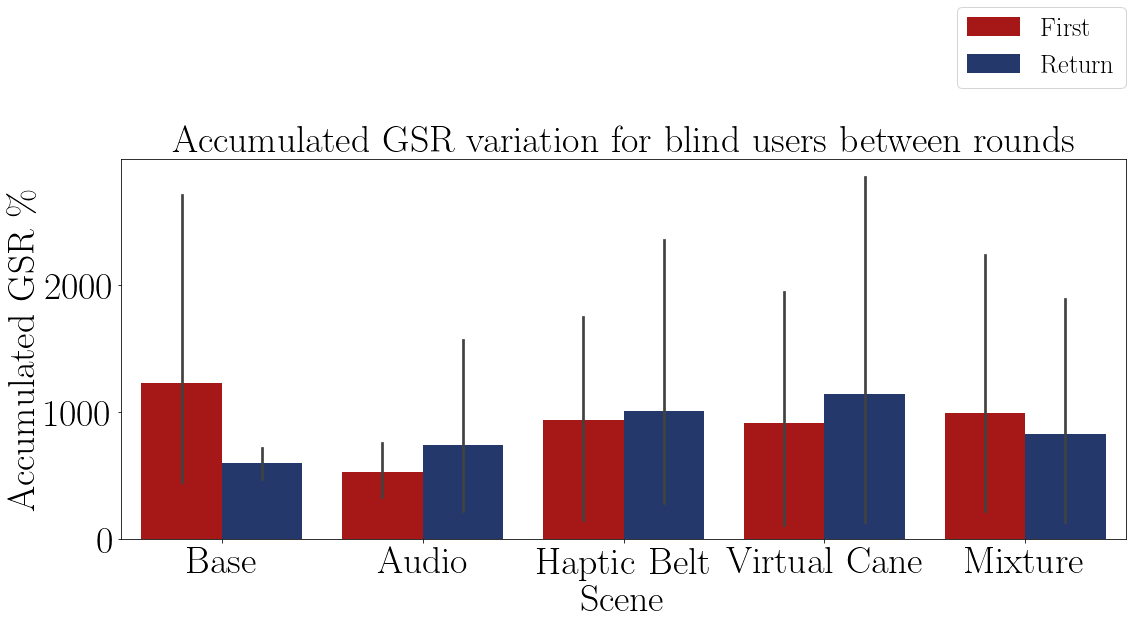
\includegraphics[width = 0.8\linewidth]{Resultados/GSR/Figuras/png/barplot_gsr_sum_scene_blind.png}
%        %\resizebox{0.8\linewidth}{!}{
%        %%% Creator: Matplotlib, PGF backend
%%
%% To include the figure in your LaTeX document, write
%%   \input{<filename>.pgf}
%%
%% Make sure the required packages are loaded in your preamble
%%   \usepackage{pgf}
%%
%% Figures using additional raster images can only be included by \input if
%% they are in the same directory as the main LaTeX file. For loading figures
%% from other directories you can use the `import` package
%%   \usepackage{import}
%%
%% and then include the figures with
%%   \import{<path to file>}{<filename>.pgf}
%%
%% Matplotlib used the following preamble
%%   \usepackage{fontspec}
%%
\begingroup%
\makeatletter%
\begin{pgfpicture}%
\pgfpathrectangle{\pgfpointorigin}{\pgfqpoint{15.369508in}{8.690562in}}%
\pgfusepath{use as bounding box, clip}%
\begin{pgfscope}%
\pgfsetbuttcap%
\pgfsetmiterjoin%
\pgfsetlinewidth{0.000000pt}%
\definecolor{currentstroke}{rgb}{1.000000,1.000000,1.000000}%
\pgfsetstrokecolor{currentstroke}%
\pgfsetstrokeopacity{0.000000}%
\pgfsetdash{}{0pt}%
\pgfpathmoveto{\pgfqpoint{0.000000in}{-0.000000in}}%
\pgfpathlineto{\pgfqpoint{15.369508in}{-0.000000in}}%
\pgfpathlineto{\pgfqpoint{15.369508in}{8.690562in}}%
\pgfpathlineto{\pgfqpoint{0.000000in}{8.690562in}}%
\pgfpathclose%
\pgfusepath{}%
\end{pgfscope}%
\begin{pgfscope}%
\pgfsetbuttcap%
\pgfsetmiterjoin%
\definecolor{currentfill}{rgb}{1.000000,1.000000,1.000000}%
\pgfsetfillcolor{currentfill}%
\pgfsetlinewidth{0.000000pt}%
\definecolor{currentstroke}{rgb}{0.000000,0.000000,0.000000}%
\pgfsetstrokecolor{currentstroke}%
\pgfsetstrokeopacity{0.000000}%
\pgfsetdash{}{0pt}%
\pgfpathmoveto{\pgfqpoint{1.319508in}{1.191562in}}%
\pgfpathlineto{\pgfqpoint{15.269508in}{1.191562in}}%
\pgfpathlineto{\pgfqpoint{15.269508in}{6.476562in}}%
\pgfpathlineto{\pgfqpoint{1.319508in}{6.476562in}}%
\pgfpathclose%
\pgfusepath{fill}%
\end{pgfscope}%
\begin{pgfscope}%
\pgfpathrectangle{\pgfqpoint{1.319508in}{1.191562in}}{\pgfqpoint{13.950000in}{5.285000in}}%
\pgfusepath{clip}%
\pgfsetbuttcap%
\pgfsetmiterjoin%
\definecolor{currentfill}{rgb}{0.651961,0.093137,0.093137}%
\pgfsetfillcolor{currentfill}%
\pgfsetlinewidth{0.000000pt}%
\definecolor{currentstroke}{rgb}{0.000000,0.000000,0.000000}%
\pgfsetstrokecolor{currentstroke}%
\pgfsetstrokeopacity{0.000000}%
\pgfsetdash{}{0pt}%
\pgfpathmoveto{\pgfqpoint{1.598508in}{5.432025in}}%
\pgfpathlineto{\pgfqpoint{2.714508in}{5.432025in}}%
\pgfpathlineto{\pgfqpoint{2.714508in}{4.583309in}}%
\pgfpathlineto{\pgfqpoint{1.598508in}{4.583309in}}%
\pgfpathclose%
\pgfusepath{fill}%
\end{pgfscope}%
\begin{pgfscope}%
\pgfpathrectangle{\pgfqpoint{1.319508in}{1.191562in}}{\pgfqpoint{13.950000in}{5.285000in}}%
\pgfusepath{clip}%
\pgfsetbuttcap%
\pgfsetmiterjoin%
\definecolor{currentfill}{rgb}{0.651961,0.093137,0.093137}%
\pgfsetfillcolor{currentfill}%
\pgfsetlinewidth{0.000000pt}%
\definecolor{currentstroke}{rgb}{0.000000,0.000000,0.000000}%
\pgfsetstrokecolor{currentstroke}%
\pgfsetstrokeopacity{0.000000}%
\pgfsetdash{}{0pt}%
\pgfpathmoveto{\pgfqpoint{4.388508in}{5.432025in}}%
\pgfpathlineto{\pgfqpoint{5.504508in}{5.432025in}}%
\pgfpathlineto{\pgfqpoint{5.504508in}{3.558465in}}%
\pgfpathlineto{\pgfqpoint{4.388508in}{3.558465in}}%
\pgfpathclose%
\pgfusepath{fill}%
\end{pgfscope}%
\begin{pgfscope}%
\pgfpathrectangle{\pgfqpoint{1.319508in}{1.191562in}}{\pgfqpoint{13.950000in}{5.285000in}}%
\pgfusepath{clip}%
\pgfsetbuttcap%
\pgfsetmiterjoin%
\definecolor{currentfill}{rgb}{0.651961,0.093137,0.093137}%
\pgfsetfillcolor{currentfill}%
\pgfsetlinewidth{0.000000pt}%
\definecolor{currentstroke}{rgb}{0.000000,0.000000,0.000000}%
\pgfsetstrokecolor{currentstroke}%
\pgfsetstrokeopacity{0.000000}%
\pgfsetdash{}{0pt}%
\pgfpathmoveto{\pgfqpoint{7.178508in}{5.432025in}}%
\pgfpathlineto{\pgfqpoint{8.294508in}{5.432025in}}%
\pgfpathlineto{\pgfqpoint{8.294508in}{4.476572in}}%
\pgfpathlineto{\pgfqpoint{7.178508in}{4.476572in}}%
\pgfpathclose%
\pgfusepath{fill}%
\end{pgfscope}%
\begin{pgfscope}%
\pgfpathrectangle{\pgfqpoint{1.319508in}{1.191562in}}{\pgfqpoint{13.950000in}{5.285000in}}%
\pgfusepath{clip}%
\pgfsetbuttcap%
\pgfsetmiterjoin%
\definecolor{currentfill}{rgb}{0.651961,0.093137,0.093137}%
\pgfsetfillcolor{currentfill}%
\pgfsetlinewidth{0.000000pt}%
\definecolor{currentstroke}{rgb}{0.000000,0.000000,0.000000}%
\pgfsetstrokecolor{currentstroke}%
\pgfsetstrokeopacity{0.000000}%
\pgfsetdash{}{0pt}%
\pgfpathmoveto{\pgfqpoint{9.968508in}{5.432025in}}%
\pgfpathlineto{\pgfqpoint{11.084508in}{5.432025in}}%
\pgfpathlineto{\pgfqpoint{11.084508in}{3.778608in}}%
\pgfpathlineto{\pgfqpoint{9.968508in}{3.778608in}}%
\pgfpathclose%
\pgfusepath{fill}%
\end{pgfscope}%
\begin{pgfscope}%
\pgfpathrectangle{\pgfqpoint{1.319508in}{1.191562in}}{\pgfqpoint{13.950000in}{5.285000in}}%
\pgfusepath{clip}%
\pgfsetbuttcap%
\pgfsetmiterjoin%
\definecolor{currentfill}{rgb}{0.651961,0.093137,0.093137}%
\pgfsetfillcolor{currentfill}%
\pgfsetlinewidth{0.000000pt}%
\definecolor{currentstroke}{rgb}{0.000000,0.000000,0.000000}%
\pgfsetstrokecolor{currentstroke}%
\pgfsetstrokeopacity{0.000000}%
\pgfsetdash{}{0pt}%
\pgfpathmoveto{\pgfqpoint{12.758508in}{5.432025in}}%
\pgfpathlineto{\pgfqpoint{13.874508in}{5.432025in}}%
\pgfpathlineto{\pgfqpoint{13.874508in}{4.339698in}}%
\pgfpathlineto{\pgfqpoint{12.758508in}{4.339698in}}%
\pgfpathclose%
\pgfusepath{fill}%
\end{pgfscope}%
\begin{pgfscope}%
\pgfpathrectangle{\pgfqpoint{1.319508in}{1.191562in}}{\pgfqpoint{13.950000in}{5.285000in}}%
\pgfusepath{clip}%
\pgfsetbuttcap%
\pgfsetmiterjoin%
\definecolor{currentfill}{rgb}{0.144608,0.218137,0.424020}%
\pgfsetfillcolor{currentfill}%
\pgfsetlinewidth{0.000000pt}%
\definecolor{currentstroke}{rgb}{0.000000,0.000000,0.000000}%
\pgfsetstrokecolor{currentstroke}%
\pgfsetstrokeopacity{0.000000}%
\pgfsetdash{}{0pt}%
\pgfpathmoveto{\pgfqpoint{2.714508in}{5.432025in}}%
\pgfpathlineto{\pgfqpoint{3.830508in}{5.432025in}}%
\pgfpathlineto{\pgfqpoint{3.830508in}{4.506389in}}%
\pgfpathlineto{\pgfqpoint{2.714508in}{4.506389in}}%
\pgfpathclose%
\pgfusepath{fill}%
\end{pgfscope}%
\begin{pgfscope}%
\pgfpathrectangle{\pgfqpoint{1.319508in}{1.191562in}}{\pgfqpoint{13.950000in}{5.285000in}}%
\pgfusepath{clip}%
\pgfsetbuttcap%
\pgfsetmiterjoin%
\definecolor{currentfill}{rgb}{0.144608,0.218137,0.424020}%
\pgfsetfillcolor{currentfill}%
\pgfsetlinewidth{0.000000pt}%
\definecolor{currentstroke}{rgb}{0.000000,0.000000,0.000000}%
\pgfsetstrokecolor{currentstroke}%
\pgfsetstrokeopacity{0.000000}%
\pgfsetdash{}{0pt}%
\pgfpathmoveto{\pgfqpoint{5.504508in}{5.432025in}}%
\pgfpathlineto{\pgfqpoint{6.620508in}{5.432025in}}%
\pgfpathlineto{\pgfqpoint{6.620508in}{3.808164in}}%
\pgfpathlineto{\pgfqpoint{5.504508in}{3.808164in}}%
\pgfpathclose%
\pgfusepath{fill}%
\end{pgfscope}%
\begin{pgfscope}%
\pgfpathrectangle{\pgfqpoint{1.319508in}{1.191562in}}{\pgfqpoint{13.950000in}{5.285000in}}%
\pgfusepath{clip}%
\pgfsetbuttcap%
\pgfsetmiterjoin%
\definecolor{currentfill}{rgb}{0.144608,0.218137,0.424020}%
\pgfsetfillcolor{currentfill}%
\pgfsetlinewidth{0.000000pt}%
\definecolor{currentstroke}{rgb}{0.000000,0.000000,0.000000}%
\pgfsetstrokecolor{currentstroke}%
\pgfsetstrokeopacity{0.000000}%
\pgfsetdash{}{0pt}%
\pgfpathmoveto{\pgfqpoint{8.294508in}{5.432025in}}%
\pgfpathlineto{\pgfqpoint{9.410508in}{5.432025in}}%
\pgfpathlineto{\pgfqpoint{9.410508in}{4.696413in}}%
\pgfpathlineto{\pgfqpoint{8.294508in}{4.696413in}}%
\pgfpathclose%
\pgfusepath{fill}%
\end{pgfscope}%
\begin{pgfscope}%
\pgfpathrectangle{\pgfqpoint{1.319508in}{1.191562in}}{\pgfqpoint{13.950000in}{5.285000in}}%
\pgfusepath{clip}%
\pgfsetbuttcap%
\pgfsetmiterjoin%
\definecolor{currentfill}{rgb}{0.144608,0.218137,0.424020}%
\pgfsetfillcolor{currentfill}%
\pgfsetlinewidth{0.000000pt}%
\definecolor{currentstroke}{rgb}{0.000000,0.000000,0.000000}%
\pgfsetstrokecolor{currentstroke}%
\pgfsetstrokeopacity{0.000000}%
\pgfsetdash{}{0pt}%
\pgfpathmoveto{\pgfqpoint{11.084508in}{5.432025in}}%
\pgfpathlineto{\pgfqpoint{12.200508in}{5.432025in}}%
\pgfpathlineto{\pgfqpoint{12.200508in}{4.423975in}}%
\pgfpathlineto{\pgfqpoint{11.084508in}{4.423975in}}%
\pgfpathclose%
\pgfusepath{fill}%
\end{pgfscope}%
\begin{pgfscope}%
\pgfpathrectangle{\pgfqpoint{1.319508in}{1.191562in}}{\pgfqpoint{13.950000in}{5.285000in}}%
\pgfusepath{clip}%
\pgfsetbuttcap%
\pgfsetmiterjoin%
\definecolor{currentfill}{rgb}{0.144608,0.218137,0.424020}%
\pgfsetfillcolor{currentfill}%
\pgfsetlinewidth{0.000000pt}%
\definecolor{currentstroke}{rgb}{0.000000,0.000000,0.000000}%
\pgfsetstrokecolor{currentstroke}%
\pgfsetstrokeopacity{0.000000}%
\pgfsetdash{}{0pt}%
\pgfpathmoveto{\pgfqpoint{13.874508in}{5.432025in}}%
\pgfpathlineto{\pgfqpoint{14.990508in}{5.432025in}}%
\pgfpathlineto{\pgfqpoint{14.990508in}{4.469000in}}%
\pgfpathlineto{\pgfqpoint{13.874508in}{4.469000in}}%
\pgfpathclose%
\pgfusepath{fill}%
\end{pgfscope}%
\begin{pgfscope}%
\pgfsetbuttcap%
\pgfsetroundjoin%
\definecolor{currentfill}{rgb}{0.000000,0.000000,0.000000}%
\pgfsetfillcolor{currentfill}%
\pgfsetlinewidth{0.803000pt}%
\definecolor{currentstroke}{rgb}{0.000000,0.000000,0.000000}%
\pgfsetstrokecolor{currentstroke}%
\pgfsetdash{}{0pt}%
\pgfsys@defobject{currentmarker}{\pgfqpoint{0.000000in}{-0.048611in}}{\pgfqpoint{0.000000in}{0.000000in}}{%
\pgfpathmoveto{\pgfqpoint{0.000000in}{0.000000in}}%
\pgfpathlineto{\pgfqpoint{0.000000in}{-0.048611in}}%
\pgfusepath{stroke,fill}%
}%
\begin{pgfscope}%
\pgfsys@transformshift{2.714508in}{1.191562in}%
\pgfsys@useobject{currentmarker}{}%
\end{pgfscope}%
\end{pgfscope}%
\begin{pgfscope}%
\definecolor{textcolor}{rgb}{0.000000,0.000000,0.000000}%
\pgfsetstrokecolor{textcolor}%
\pgfsetfillcolor{textcolor}%
\pgftext[x=2.714508in,y=1.094339in,,top]{\color{textcolor}\rmfamily\fontsize{38.016000}{45.619200}\selectfont Base}%
\end{pgfscope}%
\begin{pgfscope}%
\pgfsetbuttcap%
\pgfsetroundjoin%
\definecolor{currentfill}{rgb}{0.000000,0.000000,0.000000}%
\pgfsetfillcolor{currentfill}%
\pgfsetlinewidth{0.803000pt}%
\definecolor{currentstroke}{rgb}{0.000000,0.000000,0.000000}%
\pgfsetstrokecolor{currentstroke}%
\pgfsetdash{}{0pt}%
\pgfsys@defobject{currentmarker}{\pgfqpoint{0.000000in}{-0.048611in}}{\pgfqpoint{0.000000in}{0.000000in}}{%
\pgfpathmoveto{\pgfqpoint{0.000000in}{0.000000in}}%
\pgfpathlineto{\pgfqpoint{0.000000in}{-0.048611in}}%
\pgfusepath{stroke,fill}%
}%
\begin{pgfscope}%
\pgfsys@transformshift{5.504508in}{1.191562in}%
\pgfsys@useobject{currentmarker}{}%
\end{pgfscope}%
\end{pgfscope}%
\begin{pgfscope}%
\definecolor{textcolor}{rgb}{0.000000,0.000000,0.000000}%
\pgfsetstrokecolor{textcolor}%
\pgfsetfillcolor{textcolor}%
\pgftext[x=5.504508in,y=1.094339in,,top]{\color{textcolor}\rmfamily\fontsize{38.016000}{45.619200}\selectfont Audio}%
\end{pgfscope}%
\begin{pgfscope}%
\pgfsetbuttcap%
\pgfsetroundjoin%
\definecolor{currentfill}{rgb}{0.000000,0.000000,0.000000}%
\pgfsetfillcolor{currentfill}%
\pgfsetlinewidth{0.803000pt}%
\definecolor{currentstroke}{rgb}{0.000000,0.000000,0.000000}%
\pgfsetstrokecolor{currentstroke}%
\pgfsetdash{}{0pt}%
\pgfsys@defobject{currentmarker}{\pgfqpoint{0.000000in}{-0.048611in}}{\pgfqpoint{0.000000in}{0.000000in}}{%
\pgfpathmoveto{\pgfqpoint{0.000000in}{0.000000in}}%
\pgfpathlineto{\pgfqpoint{0.000000in}{-0.048611in}}%
\pgfusepath{stroke,fill}%
}%
\begin{pgfscope}%
\pgfsys@transformshift{8.294508in}{1.191562in}%
\pgfsys@useobject{currentmarker}{}%
\end{pgfscope}%
\end{pgfscope}%
\begin{pgfscope}%
\definecolor{textcolor}{rgb}{0.000000,0.000000,0.000000}%
\pgfsetstrokecolor{textcolor}%
\pgfsetfillcolor{textcolor}%
\pgftext[x=8.294508in,y=1.094339in,,top]{\color{textcolor}\rmfamily\fontsize{38.016000}{45.619200}\selectfont Haptic Belt}%
\end{pgfscope}%
\begin{pgfscope}%
\pgfsetbuttcap%
\pgfsetroundjoin%
\definecolor{currentfill}{rgb}{0.000000,0.000000,0.000000}%
\pgfsetfillcolor{currentfill}%
\pgfsetlinewidth{0.803000pt}%
\definecolor{currentstroke}{rgb}{0.000000,0.000000,0.000000}%
\pgfsetstrokecolor{currentstroke}%
\pgfsetdash{}{0pt}%
\pgfsys@defobject{currentmarker}{\pgfqpoint{0.000000in}{-0.048611in}}{\pgfqpoint{0.000000in}{0.000000in}}{%
\pgfpathmoveto{\pgfqpoint{0.000000in}{0.000000in}}%
\pgfpathlineto{\pgfqpoint{0.000000in}{-0.048611in}}%
\pgfusepath{stroke,fill}%
}%
\begin{pgfscope}%
\pgfsys@transformshift{11.084508in}{1.191562in}%
\pgfsys@useobject{currentmarker}{}%
\end{pgfscope}%
\end{pgfscope}%
\begin{pgfscope}%
\definecolor{textcolor}{rgb}{0.000000,0.000000,0.000000}%
\pgfsetstrokecolor{textcolor}%
\pgfsetfillcolor{textcolor}%
\pgftext[x=11.084508in,y=1.094339in,,top]{\color{textcolor}\rmfamily\fontsize{38.016000}{45.619200}\selectfont Virtual Cane}%
\end{pgfscope}%
\begin{pgfscope}%
\pgfsetbuttcap%
\pgfsetroundjoin%
\definecolor{currentfill}{rgb}{0.000000,0.000000,0.000000}%
\pgfsetfillcolor{currentfill}%
\pgfsetlinewidth{0.803000pt}%
\definecolor{currentstroke}{rgb}{0.000000,0.000000,0.000000}%
\pgfsetstrokecolor{currentstroke}%
\pgfsetdash{}{0pt}%
\pgfsys@defobject{currentmarker}{\pgfqpoint{0.000000in}{-0.048611in}}{\pgfqpoint{0.000000in}{0.000000in}}{%
\pgfpathmoveto{\pgfqpoint{0.000000in}{0.000000in}}%
\pgfpathlineto{\pgfqpoint{0.000000in}{-0.048611in}}%
\pgfusepath{stroke,fill}%
}%
\begin{pgfscope}%
\pgfsys@transformshift{13.874508in}{1.191562in}%
\pgfsys@useobject{currentmarker}{}%
\end{pgfscope}%
\end{pgfscope}%
\begin{pgfscope}%
\definecolor{textcolor}{rgb}{0.000000,0.000000,0.000000}%
\pgfsetstrokecolor{textcolor}%
\pgfsetfillcolor{textcolor}%
\pgftext[x=13.874508in,y=1.094339in,,top]{\color{textcolor}\rmfamily\fontsize{38.016000}{45.619200}\selectfont Mixture}%
\end{pgfscope}%
\begin{pgfscope}%
\definecolor{textcolor}{rgb}{0.000000,0.000000,0.000000}%
\pgfsetstrokecolor{textcolor}%
\pgfsetfillcolor{textcolor}%
\pgftext[x=8.294508in,y=0.569392in,,top]{\color{textcolor}\rmfamily\fontsize{38.016000}{45.619200}\selectfont Scene}%
\end{pgfscope}%
\begin{pgfscope}%
\pgfsetbuttcap%
\pgfsetroundjoin%
\definecolor{currentfill}{rgb}{0.000000,0.000000,0.000000}%
\pgfsetfillcolor{currentfill}%
\pgfsetlinewidth{0.803000pt}%
\definecolor{currentstroke}{rgb}{0.000000,0.000000,0.000000}%
\pgfsetstrokecolor{currentstroke}%
\pgfsetdash{}{0pt}%
\pgfsys@defobject{currentmarker}{\pgfqpoint{-0.048611in}{0.000000in}}{\pgfqpoint{-0.000000in}{0.000000in}}{%
\pgfpathmoveto{\pgfqpoint{-0.000000in}{0.000000in}}%
\pgfpathlineto{\pgfqpoint{-0.048611in}{0.000000in}}%
\pgfusepath{stroke,fill}%
}%
\begin{pgfscope}%
\pgfsys@transformshift{1.319508in}{1.767373in}%
\pgfsys@useobject{currentmarker}{}%
\end{pgfscope}%
\end{pgfscope}%
\begin{pgfscope}%
\definecolor{textcolor}{rgb}{0.000000,0.000000,0.000000}%
\pgfsetstrokecolor{textcolor}%
\pgfsetfillcolor{textcolor}%
\pgftext[x=0.636563in, y=1.584157in, left, base]{\color{textcolor}\rmfamily\fontsize{38.016000}{45.619200}\selectfont \(\displaystyle {\ensuremath{-}30}\)}%
\end{pgfscope}%
\begin{pgfscope}%
\pgfsetbuttcap%
\pgfsetroundjoin%
\definecolor{currentfill}{rgb}{0.000000,0.000000,0.000000}%
\pgfsetfillcolor{currentfill}%
\pgfsetlinewidth{0.803000pt}%
\definecolor{currentstroke}{rgb}{0.000000,0.000000,0.000000}%
\pgfsetstrokecolor{currentstroke}%
\pgfsetdash{}{0pt}%
\pgfsys@defobject{currentmarker}{\pgfqpoint{-0.048611in}{0.000000in}}{\pgfqpoint{-0.000000in}{0.000000in}}{%
\pgfpathmoveto{\pgfqpoint{-0.000000in}{0.000000in}}%
\pgfpathlineto{\pgfqpoint{-0.048611in}{0.000000in}}%
\pgfusepath{stroke,fill}%
}%
\begin{pgfscope}%
\pgfsys@transformshift{1.319508in}{2.988924in}%
\pgfsys@useobject{currentmarker}{}%
\end{pgfscope}%
\end{pgfscope}%
\begin{pgfscope}%
\definecolor{textcolor}{rgb}{0.000000,0.000000,0.000000}%
\pgfsetstrokecolor{textcolor}%
\pgfsetfillcolor{textcolor}%
\pgftext[x=0.636563in, y=2.805708in, left, base]{\color{textcolor}\rmfamily\fontsize{38.016000}{45.619200}\selectfont \(\displaystyle {\ensuremath{-}20}\)}%
\end{pgfscope}%
\begin{pgfscope}%
\pgfsetbuttcap%
\pgfsetroundjoin%
\definecolor{currentfill}{rgb}{0.000000,0.000000,0.000000}%
\pgfsetfillcolor{currentfill}%
\pgfsetlinewidth{0.803000pt}%
\definecolor{currentstroke}{rgb}{0.000000,0.000000,0.000000}%
\pgfsetstrokecolor{currentstroke}%
\pgfsetdash{}{0pt}%
\pgfsys@defobject{currentmarker}{\pgfqpoint{-0.048611in}{0.000000in}}{\pgfqpoint{-0.000000in}{0.000000in}}{%
\pgfpathmoveto{\pgfqpoint{-0.000000in}{0.000000in}}%
\pgfpathlineto{\pgfqpoint{-0.048611in}{0.000000in}}%
\pgfusepath{stroke,fill}%
}%
\begin{pgfscope}%
\pgfsys@transformshift{1.319508in}{4.210475in}%
\pgfsys@useobject{currentmarker}{}%
\end{pgfscope}%
\end{pgfscope}%
\begin{pgfscope}%
\definecolor{textcolor}{rgb}{0.000000,0.000000,0.000000}%
\pgfsetstrokecolor{textcolor}%
\pgfsetfillcolor{textcolor}%
\pgftext[x=0.636563in, y=4.027258in, left, base]{\color{textcolor}\rmfamily\fontsize{38.016000}{45.619200}\selectfont \(\displaystyle {\ensuremath{-}10}\)}%
\end{pgfscope}%
\begin{pgfscope}%
\pgfsetbuttcap%
\pgfsetroundjoin%
\definecolor{currentfill}{rgb}{0.000000,0.000000,0.000000}%
\pgfsetfillcolor{currentfill}%
\pgfsetlinewidth{0.803000pt}%
\definecolor{currentstroke}{rgb}{0.000000,0.000000,0.000000}%
\pgfsetstrokecolor{currentstroke}%
\pgfsetdash{}{0pt}%
\pgfsys@defobject{currentmarker}{\pgfqpoint{-0.048611in}{0.000000in}}{\pgfqpoint{-0.000000in}{0.000000in}}{%
\pgfpathmoveto{\pgfqpoint{-0.000000in}{0.000000in}}%
\pgfpathlineto{\pgfqpoint{-0.048611in}{0.000000in}}%
\pgfusepath{stroke,fill}%
}%
\begin{pgfscope}%
\pgfsys@transformshift{1.319508in}{5.432025in}%
\pgfsys@useobject{currentmarker}{}%
\end{pgfscope}%
\end{pgfscope}%
\begin{pgfscope}%
\definecolor{textcolor}{rgb}{0.000000,0.000000,0.000000}%
\pgfsetstrokecolor{textcolor}%
\pgfsetfillcolor{textcolor}%
\pgftext[x=1.063808in, y=5.248809in, left, base]{\color{textcolor}\rmfamily\fontsize{38.016000}{45.619200}\selectfont \(\displaystyle {0}\)}%
\end{pgfscope}%
\begin{pgfscope}%
\definecolor{textcolor}{rgb}{0.000000,0.000000,0.000000}%
\pgfsetstrokecolor{textcolor}%
\pgfsetfillcolor{textcolor}%
\pgftext[x=0.581008in,y=3.834062in,,bottom,rotate=90.000000]{\color{textcolor}\rmfamily\fontsize{38.016000}{45.619200}\selectfont Average BPM}%
\end{pgfscope}%
\begin{pgfscope}%
\pgfpathrectangle{\pgfqpoint{1.319508in}{1.191562in}}{\pgfqpoint{13.950000in}{5.285000in}}%
\pgfusepath{clip}%
\pgfsetrectcap%
\pgfsetroundjoin%
\pgfsetlinewidth{2.710125pt}%
\definecolor{currentstroke}{rgb}{0.260000,0.260000,0.260000}%
\pgfsetstrokecolor{currentstroke}%
\pgfsetdash{}{0pt}%
\pgfpathmoveto{\pgfqpoint{2.156508in}{2.751308in}}%
\pgfpathlineto{\pgfqpoint{2.156508in}{6.018483in}}%
\pgfusepath{stroke}%
\end{pgfscope}%
\begin{pgfscope}%
\pgfpathrectangle{\pgfqpoint{1.319508in}{1.191562in}}{\pgfqpoint{13.950000in}{5.285000in}}%
\pgfusepath{clip}%
\pgfsetrectcap%
\pgfsetroundjoin%
\pgfsetlinewidth{2.710125pt}%
\definecolor{currentstroke}{rgb}{0.260000,0.260000,0.260000}%
\pgfsetstrokecolor{currentstroke}%
\pgfsetdash{}{0pt}%
\pgfpathmoveto{\pgfqpoint{4.946508in}{1.431789in}}%
\pgfpathlineto{\pgfqpoint{4.946508in}{5.682086in}}%
\pgfusepath{stroke}%
\end{pgfscope}%
\begin{pgfscope}%
\pgfpathrectangle{\pgfqpoint{1.319508in}{1.191562in}}{\pgfqpoint{13.950000in}{5.285000in}}%
\pgfusepath{clip}%
\pgfsetrectcap%
\pgfsetroundjoin%
\pgfsetlinewidth{2.710125pt}%
\definecolor{currentstroke}{rgb}{0.260000,0.260000,0.260000}%
\pgfsetstrokecolor{currentstroke}%
\pgfsetdash{}{0pt}%
\pgfpathmoveto{\pgfqpoint{7.736508in}{2.678943in}}%
\pgfpathlineto{\pgfqpoint{7.736508in}{6.236334in}}%
\pgfusepath{stroke}%
\end{pgfscope}%
\begin{pgfscope}%
\pgfpathrectangle{\pgfqpoint{1.319508in}{1.191562in}}{\pgfqpoint{13.950000in}{5.285000in}}%
\pgfusepath{clip}%
\pgfsetrectcap%
\pgfsetroundjoin%
\pgfsetlinewidth{2.710125pt}%
\definecolor{currentstroke}{rgb}{0.260000,0.260000,0.260000}%
\pgfsetstrokecolor{currentstroke}%
\pgfsetdash{}{0pt}%
\pgfpathmoveto{\pgfqpoint{10.526508in}{2.047721in}}%
\pgfpathlineto{\pgfqpoint{10.526508in}{5.510294in}}%
\pgfusepath{stroke}%
\end{pgfscope}%
\begin{pgfscope}%
\pgfpathrectangle{\pgfqpoint{1.319508in}{1.191562in}}{\pgfqpoint{13.950000in}{5.285000in}}%
\pgfusepath{clip}%
\pgfsetrectcap%
\pgfsetroundjoin%
\pgfsetlinewidth{2.710125pt}%
\definecolor{currentstroke}{rgb}{0.260000,0.260000,0.260000}%
\pgfsetstrokecolor{currentstroke}%
\pgfsetdash{}{0pt}%
\pgfpathmoveto{\pgfqpoint{13.316508in}{3.163834in}}%
\pgfpathlineto{\pgfqpoint{13.316508in}{5.543100in}}%
\pgfusepath{stroke}%
\end{pgfscope}%
\begin{pgfscope}%
\pgfpathrectangle{\pgfqpoint{1.319508in}{1.191562in}}{\pgfqpoint{13.950000in}{5.285000in}}%
\pgfusepath{clip}%
\pgfsetrectcap%
\pgfsetroundjoin%
\pgfsetlinewidth{2.710125pt}%
\definecolor{currentstroke}{rgb}{0.260000,0.260000,0.260000}%
\pgfsetstrokecolor{currentstroke}%
\pgfsetdash{}{0pt}%
\pgfpathmoveto{\pgfqpoint{3.272508in}{3.222854in}}%
\pgfpathlineto{\pgfqpoint{3.272508in}{5.709606in}}%
\pgfusepath{stroke}%
\end{pgfscope}%
\begin{pgfscope}%
\pgfpathrectangle{\pgfqpoint{1.319508in}{1.191562in}}{\pgfqpoint{13.950000in}{5.285000in}}%
\pgfusepath{clip}%
\pgfsetrectcap%
\pgfsetroundjoin%
\pgfsetlinewidth{2.710125pt}%
\definecolor{currentstroke}{rgb}{0.260000,0.260000,0.260000}%
\pgfsetstrokecolor{currentstroke}%
\pgfsetdash{}{0pt}%
\pgfpathmoveto{\pgfqpoint{6.062508in}{1.933256in}}%
\pgfpathlineto{\pgfqpoint{6.062508in}{5.541904in}}%
\pgfusepath{stroke}%
\end{pgfscope}%
\begin{pgfscope}%
\pgfpathrectangle{\pgfqpoint{1.319508in}{1.191562in}}{\pgfqpoint{13.950000in}{5.285000in}}%
\pgfusepath{clip}%
\pgfsetrectcap%
\pgfsetroundjoin%
\pgfsetlinewidth{2.710125pt}%
\definecolor{currentstroke}{rgb}{0.260000,0.260000,0.260000}%
\pgfsetstrokecolor{currentstroke}%
\pgfsetdash{}{0pt}%
\pgfpathmoveto{\pgfqpoint{8.852508in}{3.694214in}}%
\pgfpathlineto{\pgfqpoint{8.852508in}{5.935485in}}%
\pgfusepath{stroke}%
\end{pgfscope}%
\begin{pgfscope}%
\pgfpathrectangle{\pgfqpoint{1.319508in}{1.191562in}}{\pgfqpoint{13.950000in}{5.285000in}}%
\pgfusepath{clip}%
\pgfsetrectcap%
\pgfsetroundjoin%
\pgfsetlinewidth{2.710125pt}%
\definecolor{currentstroke}{rgb}{0.260000,0.260000,0.260000}%
\pgfsetstrokecolor{currentstroke}%
\pgfsetdash{}{0pt}%
\pgfpathmoveto{\pgfqpoint{11.642508in}{3.336183in}}%
\pgfpathlineto{\pgfqpoint{11.642508in}{5.657013in}}%
\pgfusepath{stroke}%
\end{pgfscope}%
\begin{pgfscope}%
\pgfpathrectangle{\pgfqpoint{1.319508in}{1.191562in}}{\pgfqpoint{13.950000in}{5.285000in}}%
\pgfusepath{clip}%
\pgfsetrectcap%
\pgfsetroundjoin%
\pgfsetlinewidth{2.710125pt}%
\definecolor{currentstroke}{rgb}{0.260000,0.260000,0.260000}%
\pgfsetstrokecolor{currentstroke}%
\pgfsetdash{}{0pt}%
\pgfpathmoveto{\pgfqpoint{14.432508in}{3.718499in}}%
\pgfpathlineto{\pgfqpoint{14.432508in}{5.571045in}}%
\pgfusepath{stroke}%
\end{pgfscope}%
\begin{pgfscope}%
\pgfsetrectcap%
\pgfsetmiterjoin%
\pgfsetlinewidth{0.803000pt}%
\definecolor{currentstroke}{rgb}{0.000000,0.000000,0.000000}%
\pgfsetstrokecolor{currentstroke}%
\pgfsetdash{}{0pt}%
\pgfpathmoveto{\pgfqpoint{1.319508in}{1.191562in}}%
\pgfpathlineto{\pgfqpoint{1.319508in}{6.476562in}}%
\pgfusepath{stroke}%
\end{pgfscope}%
\begin{pgfscope}%
\pgfsetrectcap%
\pgfsetmiterjoin%
\pgfsetlinewidth{0.803000pt}%
\definecolor{currentstroke}{rgb}{0.000000,0.000000,0.000000}%
\pgfsetstrokecolor{currentstroke}%
\pgfsetdash{}{0pt}%
\pgfpathmoveto{\pgfqpoint{15.269508in}{1.191562in}}%
\pgfpathlineto{\pgfqpoint{15.269508in}{6.476562in}}%
\pgfusepath{stroke}%
\end{pgfscope}%
\begin{pgfscope}%
\pgfsetrectcap%
\pgfsetmiterjoin%
\pgfsetlinewidth{0.803000pt}%
\definecolor{currentstroke}{rgb}{0.000000,0.000000,0.000000}%
\pgfsetstrokecolor{currentstroke}%
\pgfsetdash{}{0pt}%
\pgfpathmoveto{\pgfqpoint{1.319508in}{1.191562in}}%
\pgfpathlineto{\pgfqpoint{15.269508in}{1.191562in}}%
\pgfusepath{stroke}%
\end{pgfscope}%
\begin{pgfscope}%
\pgfsetrectcap%
\pgfsetmiterjoin%
\pgfsetlinewidth{0.803000pt}%
\definecolor{currentstroke}{rgb}{0.000000,0.000000,0.000000}%
\pgfsetstrokecolor{currentstroke}%
\pgfsetdash{}{0pt}%
\pgfpathmoveto{\pgfqpoint{1.319508in}{6.476562in}}%
\pgfpathlineto{\pgfqpoint{15.269508in}{6.476562in}}%
\pgfusepath{stroke}%
\end{pgfscope}%
\begin{pgfscope}%
\definecolor{textcolor}{rgb}{0.000000,0.000000,0.000000}%
\pgfsetstrokecolor{textcolor}%
\pgfsetfillcolor{textcolor}%
\pgftext[x=8.294508in,y=6.584273in,,base]{\color{textcolor}\rmfamily\fontsize{38.016000}{45.619200}\selectfont Average BPM score variation for blind users between rounds}%
\end{pgfscope}%
\begin{pgfscope}%
\pgfsetbuttcap%
\pgfsetmiterjoin%
\definecolor{currentfill}{rgb}{1.000000,1.000000,1.000000}%
\pgfsetfillcolor{currentfill}%
\pgfsetfillopacity{0.800000}%
\pgfsetlinewidth{1.003750pt}%
\definecolor{currentstroke}{rgb}{0.800000,0.800000,0.800000}%
\pgfsetstrokecolor{currentstroke}%
\pgfsetstrokeopacity{0.800000}%
\pgfsetdash{}{0pt}%
\pgfpathmoveto{\pgfqpoint{12.990308in}{7.457562in}}%
\pgfpathlineto{\pgfqpoint{15.196175in}{7.457562in}}%
\pgfpathquadraticcurveto{\pgfqpoint{15.269508in}{7.457562in}}{\pgfqpoint{15.269508in}{7.530896in}}%
\pgfpathlineto{\pgfqpoint{15.269508in}{8.517228in}}%
\pgfpathquadraticcurveto{\pgfqpoint{15.269508in}{8.590562in}}{\pgfqpoint{15.196175in}{8.590562in}}%
\pgfpathlineto{\pgfqpoint{12.990308in}{8.590562in}}%
\pgfpathquadraticcurveto{\pgfqpoint{12.916975in}{8.590562in}}{\pgfqpoint{12.916975in}{8.517228in}}%
\pgfpathlineto{\pgfqpoint{12.916975in}{7.530896in}}%
\pgfpathquadraticcurveto{\pgfqpoint{12.916975in}{7.457562in}}{\pgfqpoint{12.990308in}{7.457562in}}%
\pgfpathclose%
\pgfusepath{stroke,fill}%
\end{pgfscope}%
\begin{pgfscope}%
\pgfsetbuttcap%
\pgfsetmiterjoin%
\definecolor{currentfill}{rgb}{0.651961,0.093137,0.093137}%
\pgfsetfillcolor{currentfill}%
\pgfsetlinewidth{0.000000pt}%
\definecolor{currentstroke}{rgb}{0.000000,0.000000,0.000000}%
\pgfsetstrokecolor{currentstroke}%
\pgfsetstrokeopacity{0.000000}%
\pgfsetdash{}{0pt}%
\pgfpathmoveto{\pgfqpoint{13.063642in}{8.187228in}}%
\pgfpathlineto{\pgfqpoint{13.796975in}{8.187228in}}%
\pgfpathlineto{\pgfqpoint{13.796975in}{8.443895in}}%
\pgfpathlineto{\pgfqpoint{13.063642in}{8.443895in}}%
\pgfpathclose%
\pgfusepath{fill}%
\end{pgfscope}%
\begin{pgfscope}%
\definecolor{textcolor}{rgb}{0.000000,0.000000,0.000000}%
\pgfsetstrokecolor{textcolor}%
\pgfsetfillcolor{textcolor}%
\pgftext[x=14.090308in,y=8.187228in,left,base]{\color{textcolor}\rmfamily\fontsize{26.400000}{31.680000}\selectfont First}%
\end{pgfscope}%
\begin{pgfscope}%
\pgfsetbuttcap%
\pgfsetmiterjoin%
\definecolor{currentfill}{rgb}{0.144608,0.218137,0.424020}%
\pgfsetfillcolor{currentfill}%
\pgfsetlinewidth{0.000000pt}%
\definecolor{currentstroke}{rgb}{0.000000,0.000000,0.000000}%
\pgfsetstrokecolor{currentstroke}%
\pgfsetstrokeopacity{0.000000}%
\pgfsetdash{}{0pt}%
\pgfpathmoveto{\pgfqpoint{13.063642in}{7.675729in}}%
\pgfpathlineto{\pgfqpoint{13.796975in}{7.675729in}}%
\pgfpathlineto{\pgfqpoint{13.796975in}{7.932395in}}%
\pgfpathlineto{\pgfqpoint{13.063642in}{7.932395in}}%
\pgfpathclose%
\pgfusepath{fill}%
\end{pgfscope}%
\begin{pgfscope}%
\definecolor{textcolor}{rgb}{0.000000,0.000000,0.000000}%
\pgfsetstrokecolor{textcolor}%
\pgfsetfillcolor{textcolor}%
\pgftext[x=14.090308in,y=7.675729in,left,base]{\color{textcolor}\rmfamily\fontsize{26.400000}{31.680000}\selectfont Return}%
\end{pgfscope}%
\end{pgfpicture}%
\makeatother%
\endgroup%

%        %}
%        \caption{Bar plot of the average skin conductance of the blind participants on each method.}
%        \label{fig:barplot_gsr_scene_blind}
%    \end{minipage}
%    \begin{minipage}{\textwidth}
%        \centering
%        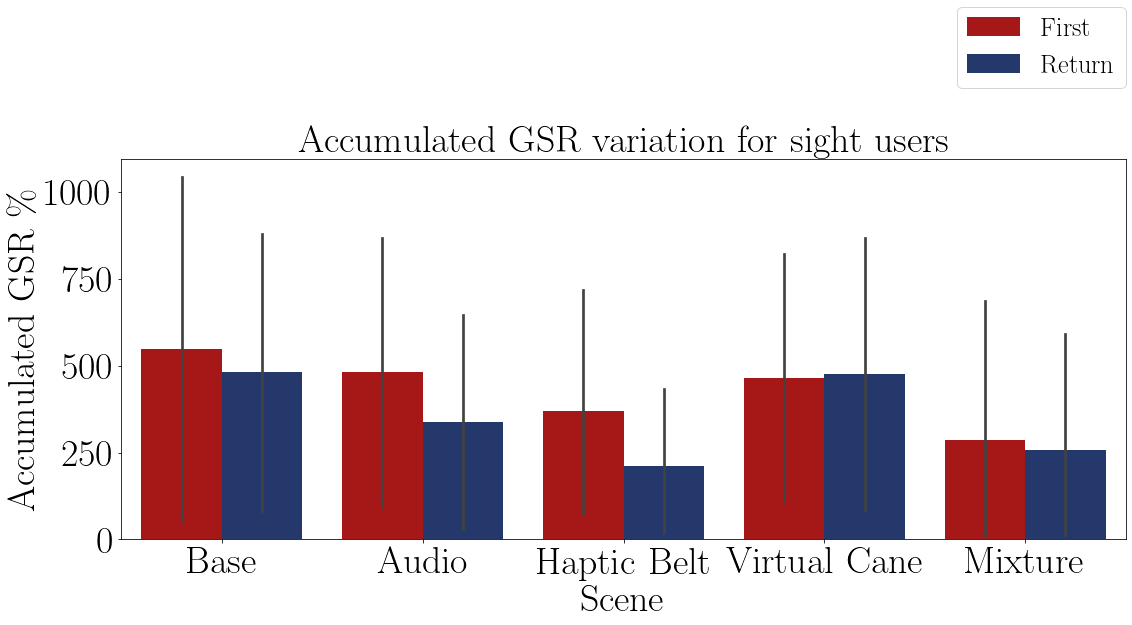
\includegraphics[width = 0.8\linewidth]{Resultados/GSR/Figuras/png/barplot_gsr_sum_scene_sight.png}
%        %\resizebox{0.6\linewidth}{!}{
%        %%% Creator: Matplotlib, PGF backend
%%
%% To include the figure in your LaTeX document, write
%%   \input{<filename>.pgf}
%%
%% Make sure the required packages are loaded in your preamble
%%   \usepackage{pgf}
%%
%% Figures using additional raster images can only be included by \input if
%% they are in the same directory as the main LaTeX file. For loading figures
%% from other directories you can use the `import` package
%%   \usepackage{import}
%%
%% and then include the figures with
%%   \import{<path to file>}{<filename>.pgf}
%%
%% Matplotlib used the following preamble
%%   \usepackage{fontspec}
%%
\begingroup%
\makeatletter%
\begin{pgfpicture}%
\pgfpathrectangle{\pgfpointorigin}{\pgfqpoint{15.281396in}{8.690562in}}%
\pgfusepath{use as bounding box, clip}%
\begin{pgfscope}%
\pgfsetbuttcap%
\pgfsetmiterjoin%
\pgfsetlinewidth{0.000000pt}%
\definecolor{currentstroke}{rgb}{1.000000,1.000000,1.000000}%
\pgfsetstrokecolor{currentstroke}%
\pgfsetstrokeopacity{0.000000}%
\pgfsetdash{}{0pt}%
\pgfpathmoveto{\pgfqpoint{0.000000in}{-0.000000in}}%
\pgfpathlineto{\pgfqpoint{15.281396in}{-0.000000in}}%
\pgfpathlineto{\pgfqpoint{15.281396in}{8.690562in}}%
\pgfpathlineto{\pgfqpoint{0.000000in}{8.690562in}}%
\pgfpathclose%
\pgfusepath{}%
\end{pgfscope}%
\begin{pgfscope}%
\pgfsetbuttcap%
\pgfsetmiterjoin%
\definecolor{currentfill}{rgb}{1.000000,1.000000,1.000000}%
\pgfsetfillcolor{currentfill}%
\pgfsetlinewidth{0.000000pt}%
\definecolor{currentstroke}{rgb}{0.000000,0.000000,0.000000}%
\pgfsetstrokecolor{currentstroke}%
\pgfsetstrokeopacity{0.000000}%
\pgfsetdash{}{0pt}%
\pgfpathmoveto{\pgfqpoint{1.231396in}{1.191562in}}%
\pgfpathlineto{\pgfqpoint{15.181396in}{1.191562in}}%
\pgfpathlineto{\pgfqpoint{15.181396in}{6.476562in}}%
\pgfpathlineto{\pgfqpoint{1.231396in}{6.476562in}}%
\pgfpathclose%
\pgfusepath{fill}%
\end{pgfscope}%
\begin{pgfscope}%
\pgfpathrectangle{\pgfqpoint{1.231396in}{1.191562in}}{\pgfqpoint{13.950000in}{5.285000in}}%
\pgfusepath{clip}%
\pgfsetbuttcap%
\pgfsetmiterjoin%
\definecolor{currentfill}{rgb}{0.651961,0.093137,0.093137}%
\pgfsetfillcolor{currentfill}%
\pgfsetlinewidth{0.000000pt}%
\definecolor{currentstroke}{rgb}{0.000000,0.000000,0.000000}%
\pgfsetstrokecolor{currentstroke}%
\pgfsetstrokeopacity{0.000000}%
\pgfsetdash{}{0pt}%
\pgfpathmoveto{\pgfqpoint{1.510396in}{1.191562in}}%
\pgfpathlineto{\pgfqpoint{2.626396in}{1.191562in}}%
\pgfpathlineto{\pgfqpoint{2.626396in}{3.511932in}}%
\pgfpathlineto{\pgfqpoint{1.510396in}{3.511932in}}%
\pgfpathclose%
\pgfusepath{fill}%
\end{pgfscope}%
\begin{pgfscope}%
\pgfpathrectangle{\pgfqpoint{1.231396in}{1.191562in}}{\pgfqpoint{13.950000in}{5.285000in}}%
\pgfusepath{clip}%
\pgfsetbuttcap%
\pgfsetmiterjoin%
\definecolor{currentfill}{rgb}{0.651961,0.093137,0.093137}%
\pgfsetfillcolor{currentfill}%
\pgfsetlinewidth{0.000000pt}%
\definecolor{currentstroke}{rgb}{0.000000,0.000000,0.000000}%
\pgfsetstrokecolor{currentstroke}%
\pgfsetstrokeopacity{0.000000}%
\pgfsetdash{}{0pt}%
\pgfpathmoveto{\pgfqpoint{4.300396in}{1.191562in}}%
\pgfpathlineto{\pgfqpoint{5.416396in}{1.191562in}}%
\pgfpathlineto{\pgfqpoint{5.416396in}{3.969940in}}%
\pgfpathlineto{\pgfqpoint{4.300396in}{3.969940in}}%
\pgfpathclose%
\pgfusepath{fill}%
\end{pgfscope}%
\begin{pgfscope}%
\pgfpathrectangle{\pgfqpoint{1.231396in}{1.191562in}}{\pgfqpoint{13.950000in}{5.285000in}}%
\pgfusepath{clip}%
\pgfsetbuttcap%
\pgfsetmiterjoin%
\definecolor{currentfill}{rgb}{0.651961,0.093137,0.093137}%
\pgfsetfillcolor{currentfill}%
\pgfsetlinewidth{0.000000pt}%
\definecolor{currentstroke}{rgb}{0.000000,0.000000,0.000000}%
\pgfsetstrokecolor{currentstroke}%
\pgfsetstrokeopacity{0.000000}%
\pgfsetdash{}{0pt}%
\pgfpathmoveto{\pgfqpoint{7.090396in}{1.191562in}}%
\pgfpathlineto{\pgfqpoint{8.206396in}{1.191562in}}%
\pgfpathlineto{\pgfqpoint{8.206396in}{4.086914in}}%
\pgfpathlineto{\pgfqpoint{7.090396in}{4.086914in}}%
\pgfpathclose%
\pgfusepath{fill}%
\end{pgfscope}%
\begin{pgfscope}%
\pgfpathrectangle{\pgfqpoint{1.231396in}{1.191562in}}{\pgfqpoint{13.950000in}{5.285000in}}%
\pgfusepath{clip}%
\pgfsetbuttcap%
\pgfsetmiterjoin%
\definecolor{currentfill}{rgb}{0.651961,0.093137,0.093137}%
\pgfsetfillcolor{currentfill}%
\pgfsetlinewidth{0.000000pt}%
\definecolor{currentstroke}{rgb}{0.000000,0.000000,0.000000}%
\pgfsetstrokecolor{currentstroke}%
\pgfsetstrokeopacity{0.000000}%
\pgfsetdash{}{0pt}%
\pgfpathmoveto{\pgfqpoint{9.880396in}{1.191562in}}%
\pgfpathlineto{\pgfqpoint{10.996396in}{1.191562in}}%
\pgfpathlineto{\pgfqpoint{10.996396in}{4.043061in}}%
\pgfpathlineto{\pgfqpoint{9.880396in}{4.043061in}}%
\pgfpathclose%
\pgfusepath{fill}%
\end{pgfscope}%
\begin{pgfscope}%
\pgfpathrectangle{\pgfqpoint{1.231396in}{1.191562in}}{\pgfqpoint{13.950000in}{5.285000in}}%
\pgfusepath{clip}%
\pgfsetbuttcap%
\pgfsetmiterjoin%
\definecolor{currentfill}{rgb}{0.651961,0.093137,0.093137}%
\pgfsetfillcolor{currentfill}%
\pgfsetlinewidth{0.000000pt}%
\definecolor{currentstroke}{rgb}{0.000000,0.000000,0.000000}%
\pgfsetstrokecolor{currentstroke}%
\pgfsetstrokeopacity{0.000000}%
\pgfsetdash{}{0pt}%
\pgfpathmoveto{\pgfqpoint{12.670396in}{1.191562in}}%
\pgfpathlineto{\pgfqpoint{13.786396in}{1.191562in}}%
\pgfpathlineto{\pgfqpoint{13.786396in}{3.591458in}}%
\pgfpathlineto{\pgfqpoint{12.670396in}{3.591458in}}%
\pgfpathclose%
\pgfusepath{fill}%
\end{pgfscope}%
\begin{pgfscope}%
\pgfpathrectangle{\pgfqpoint{1.231396in}{1.191562in}}{\pgfqpoint{13.950000in}{5.285000in}}%
\pgfusepath{clip}%
\pgfsetbuttcap%
\pgfsetmiterjoin%
\definecolor{currentfill}{rgb}{0.144608,0.218137,0.424020}%
\pgfsetfillcolor{currentfill}%
\pgfsetlinewidth{0.000000pt}%
\definecolor{currentstroke}{rgb}{0.000000,0.000000,0.000000}%
\pgfsetstrokecolor{currentstroke}%
\pgfsetstrokeopacity{0.000000}%
\pgfsetdash{}{0pt}%
\pgfpathmoveto{\pgfqpoint{2.626396in}{1.191562in}}%
\pgfpathlineto{\pgfqpoint{3.742396in}{1.191562in}}%
\pgfpathlineto{\pgfqpoint{3.742396in}{3.690373in}}%
\pgfpathlineto{\pgfqpoint{2.626396in}{3.690373in}}%
\pgfpathclose%
\pgfusepath{fill}%
\end{pgfscope}%
\begin{pgfscope}%
\pgfpathrectangle{\pgfqpoint{1.231396in}{1.191562in}}{\pgfqpoint{13.950000in}{5.285000in}}%
\pgfusepath{clip}%
\pgfsetbuttcap%
\pgfsetmiterjoin%
\definecolor{currentfill}{rgb}{0.144608,0.218137,0.424020}%
\pgfsetfillcolor{currentfill}%
\pgfsetlinewidth{0.000000pt}%
\definecolor{currentstroke}{rgb}{0.000000,0.000000,0.000000}%
\pgfsetstrokecolor{currentstroke}%
\pgfsetstrokeopacity{0.000000}%
\pgfsetdash{}{0pt}%
\pgfpathmoveto{\pgfqpoint{5.416396in}{1.191562in}}%
\pgfpathlineto{\pgfqpoint{6.532396in}{1.191562in}}%
\pgfpathlineto{\pgfqpoint{6.532396in}{4.013591in}}%
\pgfpathlineto{\pgfqpoint{5.416396in}{4.013591in}}%
\pgfpathclose%
\pgfusepath{fill}%
\end{pgfscope}%
\begin{pgfscope}%
\pgfpathrectangle{\pgfqpoint{1.231396in}{1.191562in}}{\pgfqpoint{13.950000in}{5.285000in}}%
\pgfusepath{clip}%
\pgfsetbuttcap%
\pgfsetmiterjoin%
\definecolor{currentfill}{rgb}{0.144608,0.218137,0.424020}%
\pgfsetfillcolor{currentfill}%
\pgfsetlinewidth{0.000000pt}%
\definecolor{currentstroke}{rgb}{0.000000,0.000000,0.000000}%
\pgfsetstrokecolor{currentstroke}%
\pgfsetstrokeopacity{0.000000}%
\pgfsetdash{}{0pt}%
\pgfpathmoveto{\pgfqpoint{8.206396in}{1.191562in}}%
\pgfpathlineto{\pgfqpoint{9.322396in}{1.191562in}}%
\pgfpathlineto{\pgfqpoint{9.322396in}{4.019938in}}%
\pgfpathlineto{\pgfqpoint{8.206396in}{4.019938in}}%
\pgfpathclose%
\pgfusepath{fill}%
\end{pgfscope}%
\begin{pgfscope}%
\pgfpathrectangle{\pgfqpoint{1.231396in}{1.191562in}}{\pgfqpoint{13.950000in}{5.285000in}}%
\pgfusepath{clip}%
\pgfsetbuttcap%
\pgfsetmiterjoin%
\definecolor{currentfill}{rgb}{0.144608,0.218137,0.424020}%
\pgfsetfillcolor{currentfill}%
\pgfsetlinewidth{0.000000pt}%
\definecolor{currentstroke}{rgb}{0.000000,0.000000,0.000000}%
\pgfsetstrokecolor{currentstroke}%
\pgfsetstrokeopacity{0.000000}%
\pgfsetdash{}{0pt}%
\pgfpathmoveto{\pgfqpoint{10.996396in}{1.191562in}}%
\pgfpathlineto{\pgfqpoint{12.112396in}{1.191562in}}%
\pgfpathlineto{\pgfqpoint{12.112396in}{4.247047in}}%
\pgfpathlineto{\pgfqpoint{10.996396in}{4.247047in}}%
\pgfpathclose%
\pgfusepath{fill}%
\end{pgfscope}%
\begin{pgfscope}%
\pgfpathrectangle{\pgfqpoint{1.231396in}{1.191562in}}{\pgfqpoint{13.950000in}{5.285000in}}%
\pgfusepath{clip}%
\pgfsetbuttcap%
\pgfsetmiterjoin%
\definecolor{currentfill}{rgb}{0.144608,0.218137,0.424020}%
\pgfsetfillcolor{currentfill}%
\pgfsetlinewidth{0.000000pt}%
\definecolor{currentstroke}{rgb}{0.000000,0.000000,0.000000}%
\pgfsetstrokecolor{currentstroke}%
\pgfsetstrokeopacity{0.000000}%
\pgfsetdash{}{0pt}%
\pgfpathmoveto{\pgfqpoint{13.786396in}{1.191562in}}%
\pgfpathlineto{\pgfqpoint{14.902396in}{1.191562in}}%
\pgfpathlineto{\pgfqpoint{14.902396in}{4.160726in}}%
\pgfpathlineto{\pgfqpoint{13.786396in}{4.160726in}}%
\pgfpathclose%
\pgfusepath{fill}%
\end{pgfscope}%
\begin{pgfscope}%
\pgfsetbuttcap%
\pgfsetroundjoin%
\definecolor{currentfill}{rgb}{0.000000,0.000000,0.000000}%
\pgfsetfillcolor{currentfill}%
\pgfsetlinewidth{0.803000pt}%
\definecolor{currentstroke}{rgb}{0.000000,0.000000,0.000000}%
\pgfsetstrokecolor{currentstroke}%
\pgfsetdash{}{0pt}%
\pgfsys@defobject{currentmarker}{\pgfqpoint{0.000000in}{-0.048611in}}{\pgfqpoint{0.000000in}{0.000000in}}{%
\pgfpathmoveto{\pgfqpoint{0.000000in}{0.000000in}}%
\pgfpathlineto{\pgfqpoint{0.000000in}{-0.048611in}}%
\pgfusepath{stroke,fill}%
}%
\begin{pgfscope}%
\pgfsys@transformshift{2.626396in}{1.191562in}%
\pgfsys@useobject{currentmarker}{}%
\end{pgfscope}%
\end{pgfscope}%
\begin{pgfscope}%
\definecolor{textcolor}{rgb}{0.000000,0.000000,0.000000}%
\pgfsetstrokecolor{textcolor}%
\pgfsetfillcolor{textcolor}%
\pgftext[x=2.626396in,y=1.094339in,,top]{\color{textcolor}\rmfamily\fontsize{38.016000}{45.619200}\selectfont Base}%
\end{pgfscope}%
\begin{pgfscope}%
\pgfsetbuttcap%
\pgfsetroundjoin%
\definecolor{currentfill}{rgb}{0.000000,0.000000,0.000000}%
\pgfsetfillcolor{currentfill}%
\pgfsetlinewidth{0.803000pt}%
\definecolor{currentstroke}{rgb}{0.000000,0.000000,0.000000}%
\pgfsetstrokecolor{currentstroke}%
\pgfsetdash{}{0pt}%
\pgfsys@defobject{currentmarker}{\pgfqpoint{0.000000in}{-0.048611in}}{\pgfqpoint{0.000000in}{0.000000in}}{%
\pgfpathmoveto{\pgfqpoint{0.000000in}{0.000000in}}%
\pgfpathlineto{\pgfqpoint{0.000000in}{-0.048611in}}%
\pgfusepath{stroke,fill}%
}%
\begin{pgfscope}%
\pgfsys@transformshift{5.416396in}{1.191562in}%
\pgfsys@useobject{currentmarker}{}%
\end{pgfscope}%
\end{pgfscope}%
\begin{pgfscope}%
\definecolor{textcolor}{rgb}{0.000000,0.000000,0.000000}%
\pgfsetstrokecolor{textcolor}%
\pgfsetfillcolor{textcolor}%
\pgftext[x=5.416396in,y=1.094339in,,top]{\color{textcolor}\rmfamily\fontsize{38.016000}{45.619200}\selectfont Audio}%
\end{pgfscope}%
\begin{pgfscope}%
\pgfsetbuttcap%
\pgfsetroundjoin%
\definecolor{currentfill}{rgb}{0.000000,0.000000,0.000000}%
\pgfsetfillcolor{currentfill}%
\pgfsetlinewidth{0.803000pt}%
\definecolor{currentstroke}{rgb}{0.000000,0.000000,0.000000}%
\pgfsetstrokecolor{currentstroke}%
\pgfsetdash{}{0pt}%
\pgfsys@defobject{currentmarker}{\pgfqpoint{0.000000in}{-0.048611in}}{\pgfqpoint{0.000000in}{0.000000in}}{%
\pgfpathmoveto{\pgfqpoint{0.000000in}{0.000000in}}%
\pgfpathlineto{\pgfqpoint{0.000000in}{-0.048611in}}%
\pgfusepath{stroke,fill}%
}%
\begin{pgfscope}%
\pgfsys@transformshift{8.206396in}{1.191562in}%
\pgfsys@useobject{currentmarker}{}%
\end{pgfscope}%
\end{pgfscope}%
\begin{pgfscope}%
\definecolor{textcolor}{rgb}{0.000000,0.000000,0.000000}%
\pgfsetstrokecolor{textcolor}%
\pgfsetfillcolor{textcolor}%
\pgftext[x=8.206396in,y=1.094339in,,top]{\color{textcolor}\rmfamily\fontsize{38.016000}{45.619200}\selectfont Haptic Belt}%
\end{pgfscope}%
\begin{pgfscope}%
\pgfsetbuttcap%
\pgfsetroundjoin%
\definecolor{currentfill}{rgb}{0.000000,0.000000,0.000000}%
\pgfsetfillcolor{currentfill}%
\pgfsetlinewidth{0.803000pt}%
\definecolor{currentstroke}{rgb}{0.000000,0.000000,0.000000}%
\pgfsetstrokecolor{currentstroke}%
\pgfsetdash{}{0pt}%
\pgfsys@defobject{currentmarker}{\pgfqpoint{0.000000in}{-0.048611in}}{\pgfqpoint{0.000000in}{0.000000in}}{%
\pgfpathmoveto{\pgfqpoint{0.000000in}{0.000000in}}%
\pgfpathlineto{\pgfqpoint{0.000000in}{-0.048611in}}%
\pgfusepath{stroke,fill}%
}%
\begin{pgfscope}%
\pgfsys@transformshift{10.996396in}{1.191562in}%
\pgfsys@useobject{currentmarker}{}%
\end{pgfscope}%
\end{pgfscope}%
\begin{pgfscope}%
\definecolor{textcolor}{rgb}{0.000000,0.000000,0.000000}%
\pgfsetstrokecolor{textcolor}%
\pgfsetfillcolor{textcolor}%
\pgftext[x=10.996396in,y=1.094339in,,top]{\color{textcolor}\rmfamily\fontsize{38.016000}{45.619200}\selectfont Virtual Cane}%
\end{pgfscope}%
\begin{pgfscope}%
\pgfsetbuttcap%
\pgfsetroundjoin%
\definecolor{currentfill}{rgb}{0.000000,0.000000,0.000000}%
\pgfsetfillcolor{currentfill}%
\pgfsetlinewidth{0.803000pt}%
\definecolor{currentstroke}{rgb}{0.000000,0.000000,0.000000}%
\pgfsetstrokecolor{currentstroke}%
\pgfsetdash{}{0pt}%
\pgfsys@defobject{currentmarker}{\pgfqpoint{0.000000in}{-0.048611in}}{\pgfqpoint{0.000000in}{0.000000in}}{%
\pgfpathmoveto{\pgfqpoint{0.000000in}{0.000000in}}%
\pgfpathlineto{\pgfqpoint{0.000000in}{-0.048611in}}%
\pgfusepath{stroke,fill}%
}%
\begin{pgfscope}%
\pgfsys@transformshift{13.786396in}{1.191562in}%
\pgfsys@useobject{currentmarker}{}%
\end{pgfscope}%
\end{pgfscope}%
\begin{pgfscope}%
\definecolor{textcolor}{rgb}{0.000000,0.000000,0.000000}%
\pgfsetstrokecolor{textcolor}%
\pgfsetfillcolor{textcolor}%
\pgftext[x=13.786396in,y=1.094339in,,top]{\color{textcolor}\rmfamily\fontsize{38.016000}{45.619200}\selectfont Mixture}%
\end{pgfscope}%
\begin{pgfscope}%
\definecolor{textcolor}{rgb}{0.000000,0.000000,0.000000}%
\pgfsetstrokecolor{textcolor}%
\pgfsetfillcolor{textcolor}%
\pgftext[x=8.206396in,y=0.569392in,,top]{\color{textcolor}\rmfamily\fontsize{38.016000}{45.619200}\selectfont Scene}%
\end{pgfscope}%
\begin{pgfscope}%
\pgfsetbuttcap%
\pgfsetroundjoin%
\definecolor{currentfill}{rgb}{0.000000,0.000000,0.000000}%
\pgfsetfillcolor{currentfill}%
\pgfsetlinewidth{0.803000pt}%
\definecolor{currentstroke}{rgb}{0.000000,0.000000,0.000000}%
\pgfsetstrokecolor{currentstroke}%
\pgfsetdash{}{0pt}%
\pgfsys@defobject{currentmarker}{\pgfqpoint{-0.048611in}{0.000000in}}{\pgfqpoint{-0.000000in}{0.000000in}}{%
\pgfpathmoveto{\pgfqpoint{-0.000000in}{0.000000in}}%
\pgfpathlineto{\pgfqpoint{-0.048611in}{0.000000in}}%
\pgfusepath{stroke,fill}%
}%
\begin{pgfscope}%
\pgfsys@transformshift{1.231396in}{1.191562in}%
\pgfsys@useobject{currentmarker}{}%
\end{pgfscope}%
\end{pgfscope}%
\begin{pgfscope}%
\definecolor{textcolor}{rgb}{0.000000,0.000000,0.000000}%
\pgfsetstrokecolor{textcolor}%
\pgfsetfillcolor{textcolor}%
\pgftext[x=0.975695in, y=1.008346in, left, base]{\color{textcolor}\rmfamily\fontsize{38.016000}{45.619200}\selectfont \(\displaystyle {0}\)}%
\end{pgfscope}%
\begin{pgfscope}%
\pgfsetbuttcap%
\pgfsetroundjoin%
\definecolor{currentfill}{rgb}{0.000000,0.000000,0.000000}%
\pgfsetfillcolor{currentfill}%
\pgfsetlinewidth{0.803000pt}%
\definecolor{currentstroke}{rgb}{0.000000,0.000000,0.000000}%
\pgfsetstrokecolor{currentstroke}%
\pgfsetdash{}{0pt}%
\pgfsys@defobject{currentmarker}{\pgfqpoint{-0.048611in}{0.000000in}}{\pgfqpoint{-0.000000in}{0.000000in}}{%
\pgfpathmoveto{\pgfqpoint{-0.000000in}{0.000000in}}%
\pgfpathlineto{\pgfqpoint{-0.048611in}{0.000000in}}%
\pgfusepath{stroke,fill}%
}%
\begin{pgfscope}%
\pgfsys@transformshift{1.231396in}{2.560159in}%
\pgfsys@useobject{currentmarker}{}%
\end{pgfscope}%
\end{pgfscope}%
\begin{pgfscope}%
\definecolor{textcolor}{rgb}{0.000000,0.000000,0.000000}%
\pgfsetstrokecolor{textcolor}%
\pgfsetfillcolor{textcolor}%
\pgftext[x=0.658739in, y=2.376942in, left, base]{\color{textcolor}\rmfamily\fontsize{38.016000}{45.619200}\selectfont \(\displaystyle {100}\)}%
\end{pgfscope}%
\begin{pgfscope}%
\pgfsetbuttcap%
\pgfsetroundjoin%
\definecolor{currentfill}{rgb}{0.000000,0.000000,0.000000}%
\pgfsetfillcolor{currentfill}%
\pgfsetlinewidth{0.803000pt}%
\definecolor{currentstroke}{rgb}{0.000000,0.000000,0.000000}%
\pgfsetstrokecolor{currentstroke}%
\pgfsetdash{}{0pt}%
\pgfsys@defobject{currentmarker}{\pgfqpoint{-0.048611in}{0.000000in}}{\pgfqpoint{-0.000000in}{0.000000in}}{%
\pgfpathmoveto{\pgfqpoint{-0.000000in}{0.000000in}}%
\pgfpathlineto{\pgfqpoint{-0.048611in}{0.000000in}}%
\pgfusepath{stroke,fill}%
}%
\begin{pgfscope}%
\pgfsys@transformshift{1.231396in}{3.928755in}%
\pgfsys@useobject{currentmarker}{}%
\end{pgfscope}%
\end{pgfscope}%
\begin{pgfscope}%
\definecolor{textcolor}{rgb}{0.000000,0.000000,0.000000}%
\pgfsetstrokecolor{textcolor}%
\pgfsetfillcolor{textcolor}%
\pgftext[x=0.658739in, y=3.745539in, left, base]{\color{textcolor}\rmfamily\fontsize{38.016000}{45.619200}\selectfont \(\displaystyle {200}\)}%
\end{pgfscope}%
\begin{pgfscope}%
\pgfsetbuttcap%
\pgfsetroundjoin%
\definecolor{currentfill}{rgb}{0.000000,0.000000,0.000000}%
\pgfsetfillcolor{currentfill}%
\pgfsetlinewidth{0.803000pt}%
\definecolor{currentstroke}{rgb}{0.000000,0.000000,0.000000}%
\pgfsetstrokecolor{currentstroke}%
\pgfsetdash{}{0pt}%
\pgfsys@defobject{currentmarker}{\pgfqpoint{-0.048611in}{0.000000in}}{\pgfqpoint{-0.000000in}{0.000000in}}{%
\pgfpathmoveto{\pgfqpoint{-0.000000in}{0.000000in}}%
\pgfpathlineto{\pgfqpoint{-0.048611in}{0.000000in}}%
\pgfusepath{stroke,fill}%
}%
\begin{pgfscope}%
\pgfsys@transformshift{1.231396in}{5.297352in}%
\pgfsys@useobject{currentmarker}{}%
\end{pgfscope}%
\end{pgfscope}%
\begin{pgfscope}%
\definecolor{textcolor}{rgb}{0.000000,0.000000,0.000000}%
\pgfsetstrokecolor{textcolor}%
\pgfsetfillcolor{textcolor}%
\pgftext[x=0.658739in, y=5.114136in, left, base]{\color{textcolor}\rmfamily\fontsize{38.016000}{45.619200}\selectfont \(\displaystyle {300}\)}%
\end{pgfscope}%
\begin{pgfscope}%
\definecolor{textcolor}{rgb}{0.000000,0.000000,0.000000}%
\pgfsetstrokecolor{textcolor}%
\pgfsetfillcolor{textcolor}%
\pgftext[x=0.603184in,y=3.834062in,,bottom,rotate=90.000000]{\color{textcolor}\rmfamily\fontsize{38.016000}{45.619200}\selectfont Average GSR \%}%
\end{pgfscope}%
\begin{pgfscope}%
\pgfpathrectangle{\pgfqpoint{1.231396in}{1.191562in}}{\pgfqpoint{13.950000in}{5.285000in}}%
\pgfusepath{clip}%
\pgfsetrectcap%
\pgfsetroundjoin%
\pgfsetlinewidth{2.710125pt}%
\definecolor{currentstroke}{rgb}{0.260000,0.260000,0.260000}%
\pgfsetstrokecolor{currentstroke}%
\pgfsetdash{}{0pt}%
\pgfpathmoveto{\pgfqpoint{2.068396in}{1.897169in}}%
\pgfpathlineto{\pgfqpoint{2.068396in}{5.126695in}}%
\pgfusepath{stroke}%
\end{pgfscope}%
\begin{pgfscope}%
\pgfpathrectangle{\pgfqpoint{1.231396in}{1.191562in}}{\pgfqpoint{13.950000in}{5.285000in}}%
\pgfusepath{clip}%
\pgfsetrectcap%
\pgfsetroundjoin%
\pgfsetlinewidth{2.710125pt}%
\definecolor{currentstroke}{rgb}{0.260000,0.260000,0.260000}%
\pgfsetstrokecolor{currentstroke}%
\pgfsetdash{}{0pt}%
\pgfpathmoveto{\pgfqpoint{4.858396in}{1.943825in}}%
\pgfpathlineto{\pgfqpoint{4.858396in}{5.444463in}}%
\pgfusepath{stroke}%
\end{pgfscope}%
\begin{pgfscope}%
\pgfpathrectangle{\pgfqpoint{1.231396in}{1.191562in}}{\pgfqpoint{13.950000in}{5.285000in}}%
\pgfusepath{clip}%
\pgfsetrectcap%
\pgfsetroundjoin%
\pgfsetlinewidth{2.710125pt}%
\definecolor{currentstroke}{rgb}{0.260000,0.260000,0.260000}%
\pgfsetstrokecolor{currentstroke}%
\pgfsetdash{}{0pt}%
\pgfpathmoveto{\pgfqpoint{7.648396in}{1.981923in}}%
\pgfpathlineto{\pgfqpoint{7.648396in}{5.839132in}}%
\pgfusepath{stroke}%
\end{pgfscope}%
\begin{pgfscope}%
\pgfpathrectangle{\pgfqpoint{1.231396in}{1.191562in}}{\pgfqpoint{13.950000in}{5.285000in}}%
\pgfusepath{clip}%
\pgfsetrectcap%
\pgfsetroundjoin%
\pgfsetlinewidth{2.710125pt}%
\definecolor{currentstroke}{rgb}{0.260000,0.260000,0.260000}%
\pgfsetstrokecolor{currentstroke}%
\pgfsetdash{}{0pt}%
\pgfpathmoveto{\pgfqpoint{10.438396in}{1.938265in}}%
\pgfpathlineto{\pgfqpoint{10.438396in}{5.917850in}}%
\pgfusepath{stroke}%
\end{pgfscope}%
\begin{pgfscope}%
\pgfpathrectangle{\pgfqpoint{1.231396in}{1.191562in}}{\pgfqpoint{13.950000in}{5.285000in}}%
\pgfusepath{clip}%
\pgfsetrectcap%
\pgfsetroundjoin%
\pgfsetlinewidth{2.710125pt}%
\definecolor{currentstroke}{rgb}{0.260000,0.260000,0.260000}%
\pgfsetstrokecolor{currentstroke}%
\pgfsetdash{}{0pt}%
\pgfpathmoveto{\pgfqpoint{13.228396in}{1.861914in}}%
\pgfpathlineto{\pgfqpoint{13.228396in}{4.872615in}}%
\pgfusepath{stroke}%
\end{pgfscope}%
\begin{pgfscope}%
\pgfpathrectangle{\pgfqpoint{1.231396in}{1.191562in}}{\pgfqpoint{13.950000in}{5.285000in}}%
\pgfusepath{clip}%
\pgfsetrectcap%
\pgfsetroundjoin%
\pgfsetlinewidth{2.710125pt}%
\definecolor{currentstroke}{rgb}{0.260000,0.260000,0.260000}%
\pgfsetstrokecolor{currentstroke}%
\pgfsetdash{}{0pt}%
\pgfpathmoveto{\pgfqpoint{3.184396in}{1.941799in}}%
\pgfpathlineto{\pgfqpoint{3.184396in}{5.115308in}}%
\pgfusepath{stroke}%
\end{pgfscope}%
\begin{pgfscope}%
\pgfpathrectangle{\pgfqpoint{1.231396in}{1.191562in}}{\pgfqpoint{13.950000in}{5.285000in}}%
\pgfusepath{clip}%
\pgfsetrectcap%
\pgfsetroundjoin%
\pgfsetlinewidth{2.710125pt}%
\definecolor{currentstroke}{rgb}{0.260000,0.260000,0.260000}%
\pgfsetstrokecolor{currentstroke}%
\pgfsetdash{}{0pt}%
\pgfpathmoveto{\pgfqpoint{5.974396in}{1.924633in}}%
\pgfpathlineto{\pgfqpoint{5.974396in}{5.658833in}}%
\pgfusepath{stroke}%
\end{pgfscope}%
\begin{pgfscope}%
\pgfpathrectangle{\pgfqpoint{1.231396in}{1.191562in}}{\pgfqpoint{13.950000in}{5.285000in}}%
\pgfusepath{clip}%
\pgfsetrectcap%
\pgfsetroundjoin%
\pgfsetlinewidth{2.710125pt}%
\definecolor{currentstroke}{rgb}{0.260000,0.260000,0.260000}%
\pgfsetstrokecolor{currentstroke}%
\pgfsetdash{}{0pt}%
\pgfpathmoveto{\pgfqpoint{8.764396in}{1.935764in}}%
\pgfpathlineto{\pgfqpoint{8.764396in}{5.859791in}}%
\pgfusepath{stroke}%
\end{pgfscope}%
\begin{pgfscope}%
\pgfpathrectangle{\pgfqpoint{1.231396in}{1.191562in}}{\pgfqpoint{13.950000in}{5.285000in}}%
\pgfusepath{clip}%
\pgfsetrectcap%
\pgfsetroundjoin%
\pgfsetlinewidth{2.710125pt}%
\definecolor{currentstroke}{rgb}{0.260000,0.260000,0.260000}%
\pgfsetstrokecolor{currentstroke}%
\pgfsetdash{}{0pt}%
\pgfpathmoveto{\pgfqpoint{11.554396in}{1.819956in}}%
\pgfpathlineto{\pgfqpoint{11.554396in}{6.224895in}}%
\pgfusepath{stroke}%
\end{pgfscope}%
\begin{pgfscope}%
\pgfpathrectangle{\pgfqpoint{1.231396in}{1.191562in}}{\pgfqpoint{13.950000in}{5.285000in}}%
\pgfusepath{clip}%
\pgfsetrectcap%
\pgfsetroundjoin%
\pgfsetlinewidth{2.710125pt}%
\definecolor{currentstroke}{rgb}{0.260000,0.260000,0.260000}%
\pgfsetstrokecolor{currentstroke}%
\pgfsetdash{}{0pt}%
\pgfpathmoveto{\pgfqpoint{14.344396in}{2.061192in}}%
\pgfpathlineto{\pgfqpoint{14.344396in}{5.973347in}}%
\pgfusepath{stroke}%
\end{pgfscope}%
\begin{pgfscope}%
\pgfsetrectcap%
\pgfsetmiterjoin%
\pgfsetlinewidth{0.803000pt}%
\definecolor{currentstroke}{rgb}{0.000000,0.000000,0.000000}%
\pgfsetstrokecolor{currentstroke}%
\pgfsetdash{}{0pt}%
\pgfpathmoveto{\pgfqpoint{1.231396in}{1.191562in}}%
\pgfpathlineto{\pgfqpoint{1.231396in}{6.476562in}}%
\pgfusepath{stroke}%
\end{pgfscope}%
\begin{pgfscope}%
\pgfsetrectcap%
\pgfsetmiterjoin%
\pgfsetlinewidth{0.803000pt}%
\definecolor{currentstroke}{rgb}{0.000000,0.000000,0.000000}%
\pgfsetstrokecolor{currentstroke}%
\pgfsetdash{}{0pt}%
\pgfpathmoveto{\pgfqpoint{15.181396in}{1.191562in}}%
\pgfpathlineto{\pgfqpoint{15.181396in}{6.476562in}}%
\pgfusepath{stroke}%
\end{pgfscope}%
\begin{pgfscope}%
\pgfsetrectcap%
\pgfsetmiterjoin%
\pgfsetlinewidth{0.803000pt}%
\definecolor{currentstroke}{rgb}{0.000000,0.000000,0.000000}%
\pgfsetstrokecolor{currentstroke}%
\pgfsetdash{}{0pt}%
\pgfpathmoveto{\pgfqpoint{1.231396in}{1.191562in}}%
\pgfpathlineto{\pgfqpoint{15.181396in}{1.191562in}}%
\pgfusepath{stroke}%
\end{pgfscope}%
\begin{pgfscope}%
\pgfsetrectcap%
\pgfsetmiterjoin%
\pgfsetlinewidth{0.803000pt}%
\definecolor{currentstroke}{rgb}{0.000000,0.000000,0.000000}%
\pgfsetstrokecolor{currentstroke}%
\pgfsetdash{}{0pt}%
\pgfpathmoveto{\pgfqpoint{1.231396in}{6.476562in}}%
\pgfpathlineto{\pgfqpoint{15.181396in}{6.476562in}}%
\pgfusepath{stroke}%
\end{pgfscope}%
\begin{pgfscope}%
\definecolor{textcolor}{rgb}{0.000000,0.000000,0.000000}%
\pgfsetstrokecolor{textcolor}%
\pgfsetfillcolor{textcolor}%
\pgftext[x=8.206396in,y=6.584273in,,base]{\color{textcolor}\rmfamily\fontsize{38.016000}{45.619200}\selectfont Average GSR variation for sight users}%
\end{pgfscope}%
\begin{pgfscope}%
\pgfsetbuttcap%
\pgfsetmiterjoin%
\definecolor{currentfill}{rgb}{1.000000,1.000000,1.000000}%
\pgfsetfillcolor{currentfill}%
\pgfsetfillopacity{0.800000}%
\pgfsetlinewidth{1.003750pt}%
\definecolor{currentstroke}{rgb}{0.800000,0.800000,0.800000}%
\pgfsetstrokecolor{currentstroke}%
\pgfsetstrokeopacity{0.800000}%
\pgfsetdash{}{0pt}%
\pgfpathmoveto{\pgfqpoint{12.902196in}{7.457562in}}%
\pgfpathlineto{\pgfqpoint{15.108062in}{7.457562in}}%
\pgfpathquadraticcurveto{\pgfqpoint{15.181396in}{7.457562in}}{\pgfqpoint{15.181396in}{7.530896in}}%
\pgfpathlineto{\pgfqpoint{15.181396in}{8.517228in}}%
\pgfpathquadraticcurveto{\pgfqpoint{15.181396in}{8.590562in}}{\pgfqpoint{15.108062in}{8.590562in}}%
\pgfpathlineto{\pgfqpoint{12.902196in}{8.590562in}}%
\pgfpathquadraticcurveto{\pgfqpoint{12.828862in}{8.590562in}}{\pgfqpoint{12.828862in}{8.517228in}}%
\pgfpathlineto{\pgfqpoint{12.828862in}{7.530896in}}%
\pgfpathquadraticcurveto{\pgfqpoint{12.828862in}{7.457562in}}{\pgfqpoint{12.902196in}{7.457562in}}%
\pgfpathclose%
\pgfusepath{stroke,fill}%
\end{pgfscope}%
\begin{pgfscope}%
\pgfsetbuttcap%
\pgfsetmiterjoin%
\definecolor{currentfill}{rgb}{0.651961,0.093137,0.093137}%
\pgfsetfillcolor{currentfill}%
\pgfsetlinewidth{0.000000pt}%
\definecolor{currentstroke}{rgb}{0.000000,0.000000,0.000000}%
\pgfsetstrokecolor{currentstroke}%
\pgfsetstrokeopacity{0.000000}%
\pgfsetdash{}{0pt}%
\pgfpathmoveto{\pgfqpoint{12.975529in}{8.187228in}}%
\pgfpathlineto{\pgfqpoint{13.708862in}{8.187228in}}%
\pgfpathlineto{\pgfqpoint{13.708862in}{8.443895in}}%
\pgfpathlineto{\pgfqpoint{12.975529in}{8.443895in}}%
\pgfpathclose%
\pgfusepath{fill}%
\end{pgfscope}%
\begin{pgfscope}%
\definecolor{textcolor}{rgb}{0.000000,0.000000,0.000000}%
\pgfsetstrokecolor{textcolor}%
\pgfsetfillcolor{textcolor}%
\pgftext[x=14.002196in,y=8.187228in,left,base]{\color{textcolor}\rmfamily\fontsize{26.400000}{31.680000}\selectfont First}%
\end{pgfscope}%
\begin{pgfscope}%
\pgfsetbuttcap%
\pgfsetmiterjoin%
\definecolor{currentfill}{rgb}{0.144608,0.218137,0.424020}%
\pgfsetfillcolor{currentfill}%
\pgfsetlinewidth{0.000000pt}%
\definecolor{currentstroke}{rgb}{0.000000,0.000000,0.000000}%
\pgfsetstrokecolor{currentstroke}%
\pgfsetstrokeopacity{0.000000}%
\pgfsetdash{}{0pt}%
\pgfpathmoveto{\pgfqpoint{12.975529in}{7.675729in}}%
\pgfpathlineto{\pgfqpoint{13.708862in}{7.675729in}}%
\pgfpathlineto{\pgfqpoint{13.708862in}{7.932395in}}%
\pgfpathlineto{\pgfqpoint{12.975529in}{7.932395in}}%
\pgfpathclose%
\pgfusepath{fill}%
\end{pgfscope}%
\begin{pgfscope}%
\definecolor{textcolor}{rgb}{0.000000,0.000000,0.000000}%
\pgfsetstrokecolor{textcolor}%
\pgfsetfillcolor{textcolor}%
\pgftext[x=14.002196in,y=7.675729in,left,base]{\color{textcolor}\rmfamily\fontsize{26.400000}{31.680000}\selectfont Return}%
\end{pgfscope}%
\end{pgfpicture}%
\makeatother%
\endgroup%
    
%        %}
%        \caption{Bar plot of the average skin conductance of the sighted participants on each method.}
%        \label{fig:barplot_gsr_scene_sight}
%    \end{minipage}
%\end{figure}

%The Figure \ref{fig:boxplot_ecg_bpm_scene} shows a comparison between both groups

%\begin{figure}[!htb]
%    %\centering
%    \begin{minipage}{.45\linewidth}
%        \centering
%        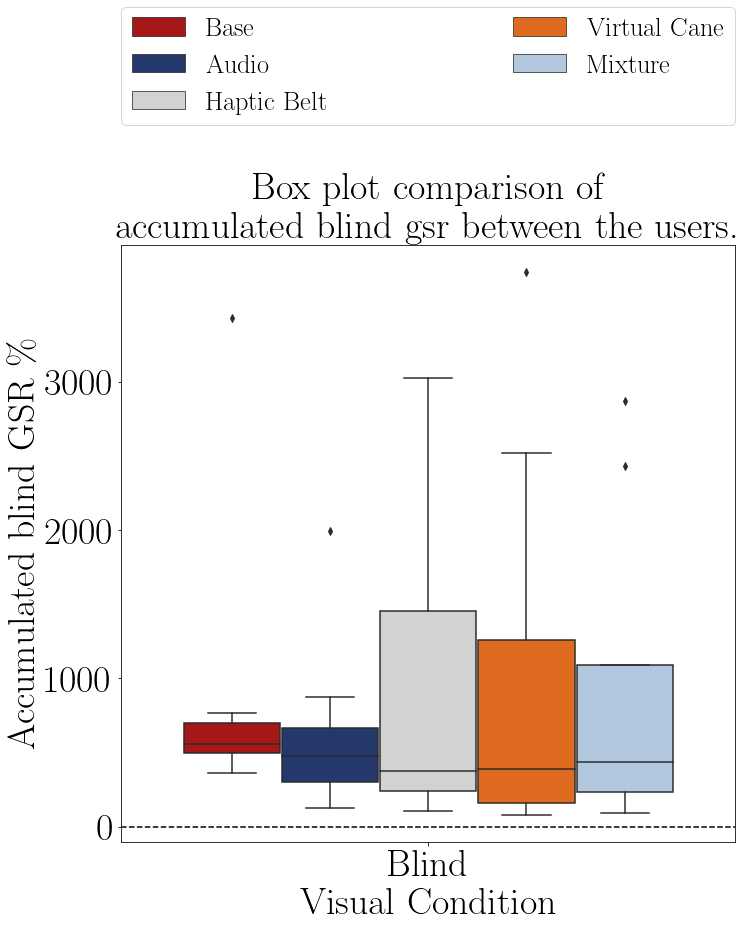
\includegraphics[width = \linewidth]{Resultados/GSR/Figuras/png/boxplot_gsr_sum_blind_scene.png}
%        \caption{Boxplot of the average skin conductace of the participants on each method.}
%        \label{fig:boxplot_gsr_scene}
%    \end{minipage}
%    \begin{minipage}{.1\linewidth}
%        \hfill
%    \end{minipage}
%    \begin{minipage}{.45\linewidth}
%        \vspace{1.8cm}
%        \centering
%        %\hspace{-4cm}
%        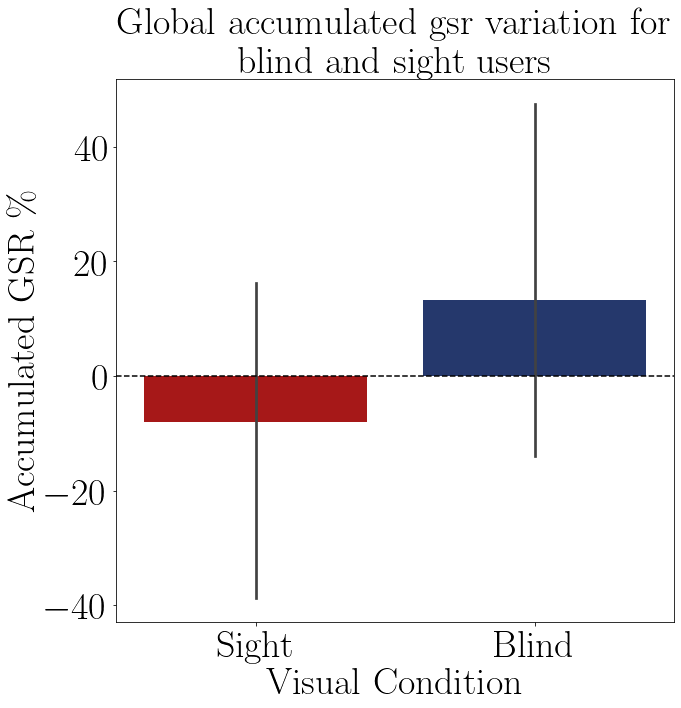
\includegraphics[width = \linewidth]{Resultados/GSR/Figuras/png/barplot_gsr_sum.png}
%        \caption{Bar plot of the average GSR of of each group.}
%        \label{fig:barplot_gsr_avg}
%    \end{minipage}
%\end{figure}
%
%\begin{figure}[!htb]
%    %\centering
%    \begin{minipage}{.45\linewidth}
%        \centering
%        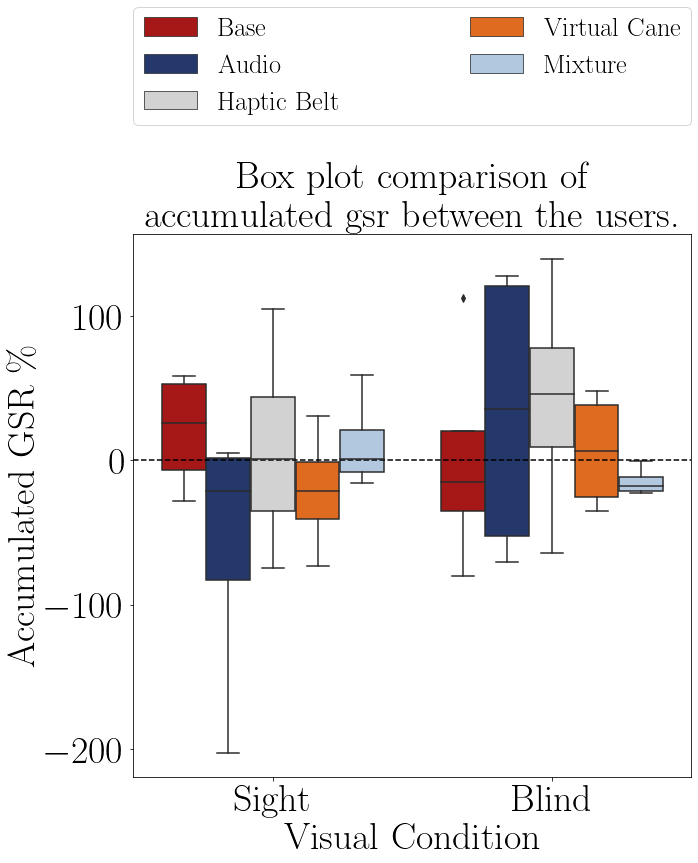
\includegraphics[width = \linewidth]{Resultados/GSR/Figuras/png/boxplot_gsr_sum_scene.png}
%        \caption{Boxplot of the average skin conductace of the participants on each method.}
%        \label{fig:boxplot_gsr_scene}
%    \end{minipage}
%    \begin{minipage}{.1\linewidth}
%        \hfill
%    \end{minipage}
%    \begin{minipage}{.45\linewidth}
%        \vspace{1.8cm}
%        \centering
%        %\hspace{-4cm}
%        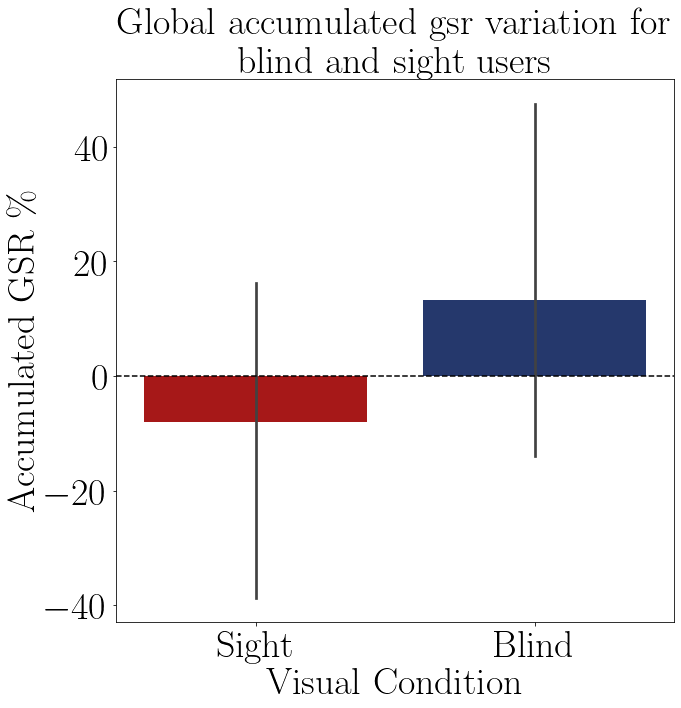
\includegraphics[width = \linewidth]{Resultados/GSR/Figuras/png/barplot_gsr_sum.png}
%        \caption{Bar plot of the average GSR of of each group.}
%        \label{fig:barplot_gsr_avg}
%    \end{minipage}
%\end{figure}

%The Table \ref{tab:gsr_avg_table_def2} shows the variation of the heartbeat in each round of each group. It is also possible to notice the same increase noticed before.

%
\begin{table}[!htb]
\centering
\caption{Accumulated GSR variation in relation to the baseline in each round.}
\label{tab:gsr_sum_table_etp}
\begin{tabular}{lllrrrrrr}
\toprule
    &       &        &      Base &     Audio & \begin{tabular}[c]{@{}l@{}}Haptic\\ Belt\end{tabular} & \begin{tabular}[c]{@{}l@{}}Virtual\\ Cane\end{tabular} &   Mixture \\
Part. & \begin{tabular}[c]{@{}l@{}}Visual\\ Condition\end{tabular} & Round &           &           &                                                       &                                                        &           \\
\midrule
001 & Sight & First &   152.6\% &   121.9\% &                                               174.0\% &                                                261.2\% &    71.9\% \\
    &       & Return &   241.4\% &   128.1\% &                                               135.4\% &                                                182.6\% &   114.5\% \\
001C & Blind & First &   578.3\% &   872.7\% &                                              2261.2\% &                                               2520.5\% &  2866.5\% \\
    &       & Return &   518.2\% &  1990.6\% &                                              3027.1\% &                                               3741.2\% &  2431.1\% \\
002C & Blind & First &  3430.8\% &   423.8\% &                                               105.0\% &                                                 75.7\% &    93.9\% \\
    &       & Return &   674.9\% &   125.9\% &                                               251.8\% &                                                102.5\% &    93.6\% \\
003 & Sight & First &   -49.9\% &    67.4\% &                                               -25.7\% &                                                -41.2\% &   -53.3\% \\
    &       & Return &   -75.6\% &   -69.0\% &                                               -52.8\% &                                                -11.2\% &   -57.7\% \\
003C & Blind & First &   361.4\% &   244.3\% &                                               206.8\% &                                                838.9\% &   646.0\% \\
    &       & Return &   767.4\% &   532.8\% &                                               325.9\% &                                                546.8\% &   514.4\% \\
004 & Sight & First &   886.0\% &   676.1\% &                                               899.3\% &                                                966.4\% &   890.9\% \\
    &       & Return &   894.0\% &   681.9\% &                                               227.2\% &                                                853.4\% &   750.0\% \\
004C & Blind & First &   539.7\% &   593.0\% &                                              1185.5\% &                                                228.6\% &   360.4\% \\
    &       & Return &   432.9\% &   316.4\% &                                               421.8\% &                                                178.2\% &   280.1\% \\
005 & Sight & First &  1198.9\% &  1060.1\% &                                               430.7\% &                                                673.9\% &   233.2\% \\
    &       & Return &   864.7\% &   609.9\% &                                               533.4\% &                                                880.6\% &   220.0\% \\
\bottomrule
\end{tabular}
\end{table}


%
%
\begin{table}[!htb]
\centering
\caption{Accumulate GSR variation in relation to the baseline grouped by participant and visual Condition.}
\label{tab:gsr_var_sum_def_blind}
\begin{tabular}{lrrrrr}
\toprule
{} &     Base &    Audio & Haptic Belt & Virtual Cane &  Mixture \\
Visual Condition &          &          &             &              &          \\
\midrule
Blind            &  913.0\% &  637.4\% &     973.1\% &     1029.0\% &  910.8\% \\
\bottomrule
\end{tabular}
\end{table}


%
%
\begin{table}[!htb]
\centering
\caption{Accumulate GSR variation in relation to the baseline grouped by participant and visual Condition.}
\label{tab:gsr_var_sum_def}
\begin{tabular}{lrrrrr}
\toprule
{} &    Base &    Audio & Haptic Belt & Virtual Cane &  Mixture \\
Visual Condition &         &          &             &              &          \\
\midrule
Blind            &   0.5\% &   32.3\% &      41.7\% &        6.7\% &  -14.6\% \\
Sight            &  20.7\% &  -59.7\% &       8.0\% &      -21.0\% &   11.5\% \\
\bottomrule
\end{tabular}
\end{table}



%The Shapiro–Wilk normality test on the Table \ref{tab:shapiro_gsr_avg} shows that only the "Audio" method is normally distributed for the "blind" sample while for the "sight" sample only the "Virtual Cane" is not normally distributed

%According to the T-Test presented in the Table \ref{tab:ttest_gsr} there is no difference in the skin conductace  frequency variation between the sample groups.


%\begin{table}[!htb]
%    \begin{minipage}{.45\linewidth}
%        
\centering
\caption{Shapiro test p-value for the gsr accumulated for each method and visual condition}
\label{tab:shapiro_gsr_sum}
\begin{tabular}{lr}
\toprule
                    Method & Shapiro P-Value \\
\midrule
        Base blinded users &         0.000** \\
        Base sighted users &           0.156 \\
       Audio blinded users &         0.015** \\
       Audio sighted users &           0.282 \\
 Haptic Belt blinded users &         0.021** \\
 Haptic Belt sighted users &           0.432 \\
Virtual Cane blinded users &         0.008** \\
Virtual Cane sighted users &           0.158 \\
     Mixture blinded users &         0.006** \\
     Mixture sighted users &           0.060 \\
\bottomrule
\end{tabular}

%    \end{minipage}
%    \hfill
%    \begin{minipage}{.45\linewidth}
%        \vspace{-2.75cm}
%        
\centering
\caption{T test p-value for the accumulated GSR on each method for blinded users versus sighted users.}
\label{tab:ttest_gsr_sum}
\begin{tabular}{lr}
\toprule
      Method &  T-Test P-Value \\
\midrule
        Base &           0.339 \\
       Audio &           0.383 \\
 Haptic Belt &           0.114 \\
Virtual Cane &           0.286 \\
     Mixture &           0.139 \\
\bottomrule
\end{tabular}

%    \end{minipage}
%\end{table}

%The Table \ref{tab:repblocanova_gsr} shows the Anova test p-value of the skin conductance frequency of the "blind" sample between the guidance methods presented in the Table \ref{tab:gsr_avg_table}. The p-value indicates that there is at least one method that is statistically equal to one of the other methods.

%
\begin{table}[!htb]
\centering
\caption{Anova p-value for the accumulated GSR score on each method for blinded users.}
\label{tab:blocanova_gsr_sum}
\begin{tabular}{lrrrrr}
\toprule
            Source &  Squared sum &  DOF & Squared average &     F & \begin{tabular}[c]{@{}l@{}}P-Value \\ $(F_{0} > F)$\end{tabular} \\
\midrule
   Between factors &   727620.618 &    4 &      181905.155 & 0.148 &                                                            0.960 \\
    Between blocks & 18855883.057 &    3 &     6285294.352 & 5.124 &                                                            0.016 \\
Experimental error & 14719563.480 &   12 &     1226630.290 &       &                                                                  \\
    Sampling Error &  6135320.519 &   20 &      306766.026 &       &                                                                  \\
             Total & 40438387.674 &   39 &                 &       &                                                                  \\
\bottomrule
\end{tabular}
\end{table}



%The Table \ref{tab:lsd_gsr} presents the conclusion of a pairwise Fisher LSD test of the blind skin conductance frequency variation between all the guidance methods. The results show that the "Virtual Cane" and the "Mixture" have different variations, but since they are not normally distributed this conclusion can not statistically be made.

%
\begin{table}[!htb]
\centering
\caption{Cross validation p-value for the accumulated GSR on each method for blinded users.}
\label{tab:lsd_gsr_sum}
\begin{tabular}{rclr}
\toprule
      \multicolumn{3}{c}{Method} &                                       Analysis \\
\midrule
              Base & $X$ & Audio &               $H_0 : \mu_{Base} = \mu_{Audio}$ \\
        Base & $X$ & Haptic Belt &         $H_0 : \mu_{Base} = \mu_{Haptic Belt}$ \\
       Base & $X$ & Virtual Cane &        $H_0 : \mu_{Base} = \mu_{Virtual Cane}$ \\
            Base & $X$ & Mixture &             $H_0 : \mu_{Base} = \mu_{Mixture}$ \\
       Audio & $X$ & Haptic Belt &        $H_0 : \mu_{Audio} = \mu_{Haptic Belt}$ \\
      Audio & $X$ & Virtual Cane &       $H_0 : \mu_{Audio} = \mu_{Virtual Cane}$ \\
           Audio & $X$ & Mixture &            $H_0 : \mu_{Audio} = \mu_{Mixture}$ \\
Haptic Belt & $X$ & Virtual Cane & $H_0 : \mu_{Haptic Belt} = \mu_{Virtual Cane}$ \\
     Haptic Belt & $X$ & Mixture &      $H_0 : \mu_{Haptic Belt} = \mu_{Mixture}$ \\
    Virtual Cane & $X$ & Mixture &     $H_0 : \mu_{Virtual Cane} = \mu_{Mixture}$ \\
\bottomrule
\end{tabular}
\end{table}



%According to the Anova test at Table \ref{tab:repblocanova_gsr} and the LSD test at \ref{tab:lsd_gsr} only the "Virtual Cane" and the "Mixture" method provoked a different reaction than the "Base" method, but since the Shapiro test at the Table \ref{tab:shapiro_gsr_avg} showed that they are not normally distributed, than this conclusion has no foundation.



\FloatBarrier

